\documentclass[letterpaper, 11pt]{article}
\usepackage[english]{babel}
\usepackage[utf8]{inputenc}
\usepackage{eurosym}
\usepackage{amsmath,amsfonts,amsthm,amssymb}
\usepackage{graphicx}
\usepackage{subcaption}
\usepackage{tabularx}
\usepackage{float}
\usepackage{placeins}
\renewcommand{\topfraction}{0.9}
\renewcommand{\bottomfraction}{0.7}
\renewcommand{\textfraction}{0.07}
\renewcommand{\floatpagefraction}{0.75}
\setcounter{topnumber}{3}
\setcounter{totalnumber}{4}
\usepackage{multirow}
\usepackage[hidelinks]{hyperref}
\usepackage[myheadings]{fullpage}
\usepackage{fancyhdr}
\usepackage{chngcntr}
\usepackage{indentfirst} 
\usepackage[top=2.2cm, bottom=3.2cm, left=2cm, right=2cm]{geometry}
\usepackage{graphicx}     
\usepackage{makecell}     
\usepackage{booktabs}      
\usepackage{threeparttable}
\usepackage{array}
\usepackage{multirow}
\usepackage[table,xcdraw]{xcolor}
\usepackage{enumerate}
\counterwithin{figure}{section}
\counterwithin{table}{section}
\counterwithin{equation}{section}

% --------------------------------------------------------------------
% Definitions (do not change this)
% --------------------------------------------------------------------
\newcommand{\HRule}[1]{\rule{\linewidth}{#1}} 	% Horizontal rule

\makeatletter							% Title
\def\printtitle{%						
    {\centering \@title\par}}
\makeatother									

\makeatletter							% Author
\def\printauthor{%					
    {\centering \large \@author}}				
\makeatother		
\graphicspath{{figures/}}

% ============================================================================
% Modelling Wind Energy Potentials and Energy Pricing Between the
% Northern and Baltic Sea
% Faisal Bindakhil · MSc Sustainable Energy Futures · Imperial College London
%
% Structure per 8_THESIS_SKELETON.md. Word budget 20,000:
%   01 Introduction        ~1,800
%   02 Literature review   ~4,500
%   03 Methodology         ~4,500
%   04 Results             ~5,500
%   05 Discussion          ~2,200
%   06 Conclusion            ~800
% Figures are referenced by file name only; all live in figures/.
% Style: no em dashes, concise, every line earns its place.
% ============================================================================

\begin{document}

% ----------------------------- title page ----------------------------------
\begin{titlepage}
\centering
% Crest shown if present in figures/; absence never blocks compilation.
\IfFileExists{figures/Imperial_College_London_crest.png}
  {
\includegraphics[height=4.5cm]{Imperial_College_London_crest.png}\\[1.2cm]}
  {\vspace*{1.5cm}}
{\Large Modelling Wind Energy Potentials and Energy Pricing\\
Between the Northern and Baltic Sea\\[1.5cm]}
{\large Faisal Bindakhil\\[0.4cm]}
A thesis presented to Imperial College London in partial fulfilment of the
requirements for the degree of Master of Science in Sustainable Energy
Futures\\[1.0cm]
Energy Futures Lab\\
\today
\end{titlepage}

% ----------------------------- front matter --------------------------------
% ============================================================================
% Abstract  (front matter, input before the table of contents)
% Structure after Jacquet: stakes and question / method / findings with
% numbers / implications. Four paragraphs, self-sufficient. No em dashes.
% ============================================================================

\section*{Abstract}

Europe's next wave of offshore wind moves from the mature North Sea into the
enclosed Baltic Sea, where wind farms generate at the same time and push down
the price they all sell at. The share of the average electricity price that a
wind farm actually receives is called its capture value, and it falls as more
wind is built. This thesis measures capture value for every electricity market
around the two seas from 2017 to 2024 and projects it to 2030 and 2040, using
open data throughout. It asks three questions: how the two seas compare today
and how they will compare once the planned wind farms are built, what causes
the loss of value and how much of it can be avoided by building the
surrounding system differently, and whether a model trained on the past can
predict a future this different, or whether a model that rebuilds the market
from its parts is required.

Two models are built and compared with each other. The first is a statistical
model, trained on eight years of observed prices at 31 offshore wind farms.
The second is a power-system model, PyPSA-Eur, which reconstructs the market
from its parts, the power plants, the transmission grid and the demand in
every hour, under the official European expansion scenarios for 2030 and 2040.
Both models are checked against observed prices before either is trusted.

Today the two regions are equal in terms of capture value: wind farms in both capture roughly 88 per cent
of the average electricity price. By 2040, with the planned buildout in place
and today's grid, Baltic farms fall to 47 per cent while North Sea farms hold
57, so the Baltic loses almost half of its present value. About half of that
loss is caused by congestion in the grid, and it can be removed: with
transmission expanded, the Baltic recovers to 66 per cent, level with the
North Sea again. The two models prove equally accurate where they can be
checked, and their estimates of capture value agree to within half a
percentage point, but beyond the observed record the statistical model returns
almost the same answer whichever future it is given, so the long-term
projection must come from the power-system model. Even with an expanded grid
the Baltic captures a quarter less than it does today, so what the planned
wind farms will be worth depends on the grid built alongside them.
\newpage
% ============================================================================
% Acknowledgements (front matter, after the abstract)
% Weighted to Ruslan Galimov, brief for Adam Hawkes and Malte Jansen.
% Restrained in tone. No em dashes.
% CHECK BEFORE SUBMISSION: names, titles and affiliations.
\section*{Acknowledgements}

My thanks go first to Dr.\ Ruslan Galimov of RWE, who proposed this project and
guided it throughout. His industrial perspective kept the work anchored to the
decisions it is meant to inform, and he repeatedly sent me back to check
something I had taken for granted. The thesis is more careful for it.

I am grateful to Prof.\ Adam Hawkes for supervising the project and for the
confidence he placed in it, and to Dr.\ Malte Jansen for a discussion early on
that shaped how I framed the value question.

Finally, thank you to my family and friends for their support over the course
of the year.
\newpage
\tableofcontents
\newpage
\listoffigures
\listoftables
\newpage

% ----------------------------- chapters ------------------------------------
% ============================================================================
% Chapter 1 · Introduction
% Style: no em dashes; concrete hook; funnel from stakes to gap to questions;
% state the gap, the contributions, the scope, and the roadmap explicitly.
% Cross-chapter references use plain "Chapter N" (thesis convention).
% ============================================================================

\section{Introduction}\label{sec:introduction}

In 2024, German day-ahead electricity prices fell below zero for 459 hours,
roughly three times the count of two years earlier
\cite{FfE2025_GermanElectricityPricesEPEX2024}. That is the structural
signature of wind at scale: the more of it a power system absorbs, the less each
additional unit earns on the wholesale market. That tension, between the ambition to build offshore wind and the
economics that erode its value as it is built, is the subject of this thesis.

A wind farm sells its electricity at the price prevailing in the hours it
happens to generate, and because wind output is correlated across a region,
those are precisely the hours in which farms produce together and depress the
price they all receive. What a farm earns per unit of electricity is therefore
the average price of its own generating hours, which sits below the market's
overall average. The fraction of the average price a farm captures in this way
is its capture value, and it declines as regional wind capacity grows, a
process called cannibalisation \cite{Hirth2013}. Because revenue is output
multiplied by the price that output sells at, capture value is increasingly
the term that decides whether an offshore project is viable.

Europe ended 2024 with roughly 36~GW of offshore wind
\cite{Colaluce2025_EuropeOffshoreWind} and plans on the order of 360~GW by 2050
\cite{EuropeanCommission2021_EUReferenceScenario2020}, a tenfold expansion
within the lifetime of a single project. Most of today's capacity
sits in the mature North Sea, where Germany alone operates 9.2~GW
\cite{OffshoreWIND2025_GermanyOffshoreCapacity}; the next wave moves east into the
enclosed Baltic, where the Marienborg Declaration targets 19.6~GW by 2030 against
a technical potential of up to 93~GW \cite{BalticWind2024_BEMIPOffshorePriorities}.
The question is no longer whether offshore wind expands, but where it
expands and what value survives once it does.

Policy makes that question more urgent: REPowerEU lifted the EU's 2030 renewable
target to 42.5\% \cite{REPowerEU2022}, the IEA and IRENA project a tripling
of global renewable capacity by 2030 \cite{IEA2024, IRENA2024}, the Draghi
report names European electricity prices a threat to industrial survival
\cite{Draghi2024}, and the 2024 market reform made the two-sided contract for
difference the default for supported capacity \cite{EUMarketReform2024}.
Each of these forces more zero-marginal-cost generation into the market, and
so deepens the erosion this thesis measures.

Yet the basin where the next wave will land has never been systematically compared
with the North Sea on the metric that decides its viability. Cannibalisation has
been quantified nationally \cite{Hirth2013} and pan-European in aggregate
\cite{Stiewe2025}, but the statistical models used absorb each market's character
into a single fitted constant. They establish that markets differ while leaving
the reason inside that constant, and they cannot be carried into a future in
which the characteristics they absorb have changed. And because investment horizons force projection, every projected capture
value in the literature rests on a single model family never validated
against another. The enclosed Baltic, earlier on its cannibalisation curve
and structurally less able to export its surplus, is the case these gaps
leave unanswered.

This thesis measures and projects the market value of offshore wind across the
open North Sea and the enclosed Baltic, entirely on open data. It asks how the
two basins compare today and how they diverge as the committed buildout is
delivered, what sets the rate at which value is lost and how much of that loss
system design can remove, and whether a model fitted to historical observation
can describe a future lying outside it or whether a model of the power system is
required. Section~\ref{sec:research_gap} states these three questions formally,
after setting out the gaps they follow from.

Answering them requires two models, because no single one can both measure the
present credibly and describe a future that has never occurred. A regression
model fitted to eight years of observed prices measures the present. A system
model, PyPSA-Eur (Python for Power System Analysis), rebuilds the market from
generation costs and the physical network and projects beyond the observed
record. Both are compared against observed capture value wherever it exists, and
that comparison decides which model is used for what
(Section~\ref{sec:design}).

On this design the thesis makes four contributions, the first of which is a
systematic North-Sea-versus-Baltic capture-value comparison at the bidding-zone
resolution where prices form, carried from today's measurement to the 2040
buildout. The
second sets the two models against observation and against each other on the
same quantity, and determines from measurement, rather than by assumption, at which point the projection should pass from one model to the other: the regression model is shown to stop answering where it cannot
extrapolate, the remaining gap is decomposed into the construction steps that
produce it, and the system model's congestion bias is corrected against
observation. The third decomposes the erosion twice, into the structural part no
grid can remove and the congestion part an optimal grid does, and into the
shares of the loss borne by the farm and by the state under the contracts that
now dominate support. The fourth folds capture value into levelised cost to give
a value-adjusted cost of energy per location, and carries it to the decision it
changes, which is where to build. The whole chain rests on open data and open
code, so every number in the thesis can be reproduced.

The study covers both basins through 31 offshore wind farms, sixteen in the North
Sea and fifteen in the Baltic, measured hourly over 2017 to 2024 and projected to
2030 and 2040 under the official European transmission-planning scenarios. The
fourteen countries bordering the two seas hold 21.1~GW of Europe's offshore
capacity today, the remainder sitting mostly in Great Britain, which lies outside
the modelled area. Figure~\ref{fig:study_farms} maps the farms.

\begin{figure}[!htb]
    \centering
    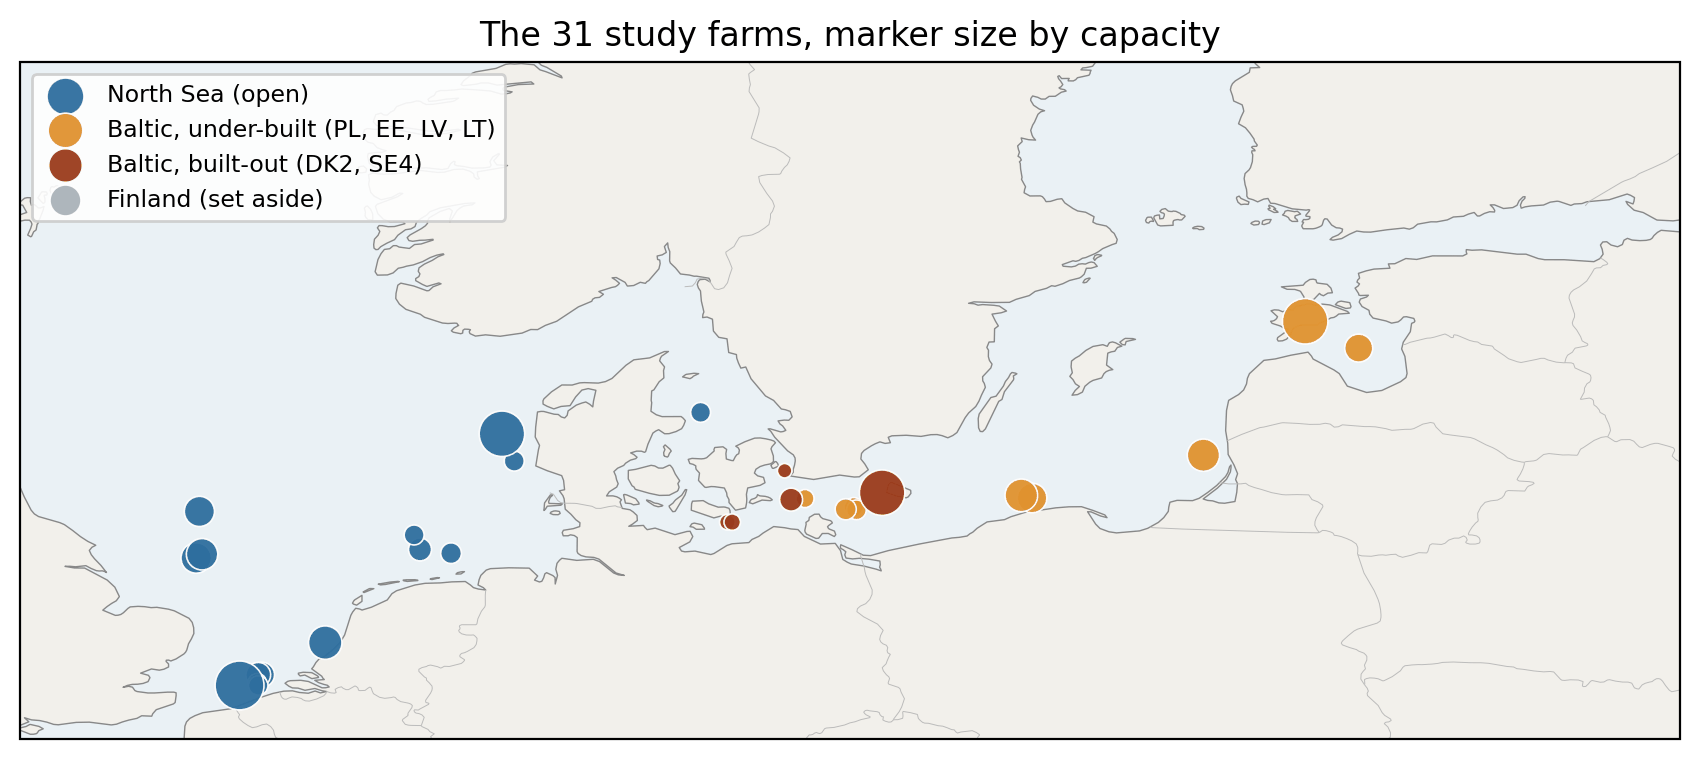
\includegraphics[width=0.92\textwidth]{fig_study_farms}
    \caption{The 31 study farms across the two basins. Marker size is
    proportional to capacity, and the farms are grouped into the four categories
    used throughout the thesis: the open North Sea fleet, the under-built Baltic
    fleet whose buildout is projected here, the built-out zones DK2 and SE4, and
    Finland, which is set aside.}
    \label{fig:study_farms}
\end{figure}
Chapter 2 builds the concepts from first principles and locates the gaps the
questions above fill. Chapter 3 develops the two models and how they are compared. Chapter 4 measures today's value, tests the two models against
observation and against each other, projects the buildout, explains what drives
the erosion, and turns the result into decisions: a break-even price per site
and a ranking of where to build. The accounting of who bears the loss is
carried in Appendix~\ref{app:portfolio}. Chapter 5 answers the three research
questions against that evidence, sets the answers against the literature, and
states the limits of the work. Chapter 6 concludes. The finding that
carries through every chapter is that cannibalisation in the Baltic is a
consequence of the system built around the basin.

\section{Background and Literature Review}\label{sec:literature}

Offshore wind is usually measured in gigawatts installed and terawatt-hours
generated. Neither quantity determines whether a wind farm earns money. A
generator is paid the price prevailing in the hours it produces, and because
wind output across a sea basin arrives together, those are precisely the hours
in which the price is lowest. This chapter builds the argument from that single
observation. Section~\ref{sec:markets} sets out how European wholesale prices
form. Section~\ref{sec:value_problem} defines the resulting value erosion and
reviews its measured magnitude. Section~\ref{sec:mitigation} asks the question
on which this thesis turns, namely whether that erosion is an inherent property
of the resource or a consequence of system design that can be reversed.
Section~\ref{sec:two_seas} contrasts the two basins under study, and
Section~\ref{sec:modelling} reviews the model families available for
answering the question. Section~\ref{sec:research_gap} states the gaps that
remain and the questions this thesis puts to them.

\subsection{Price formation in electricity markets}\label{sec:markets}

The day-ahead market, which carries 80 to 90\,\% of merchant wind revenue
\cite{Jansen2020}, clears pay-as-clear. Generators offer at short-run
marginal cost, the market operator stacks those offers into an ascending supply
curve, and every dispatched unit receives the price of the most expensive unit
required to meet demand. Wind turbines, whose fuel is free, enter at the bottom
of that stack. Additional wind shifts the supply curve to the right,
displaces the marginal thermal unit, and lowers the clearing price. This is the
merit order effect, illustrated in Figure~\ref{fig:merit_order}.

\begin{figure}[!htb]
    \centering
    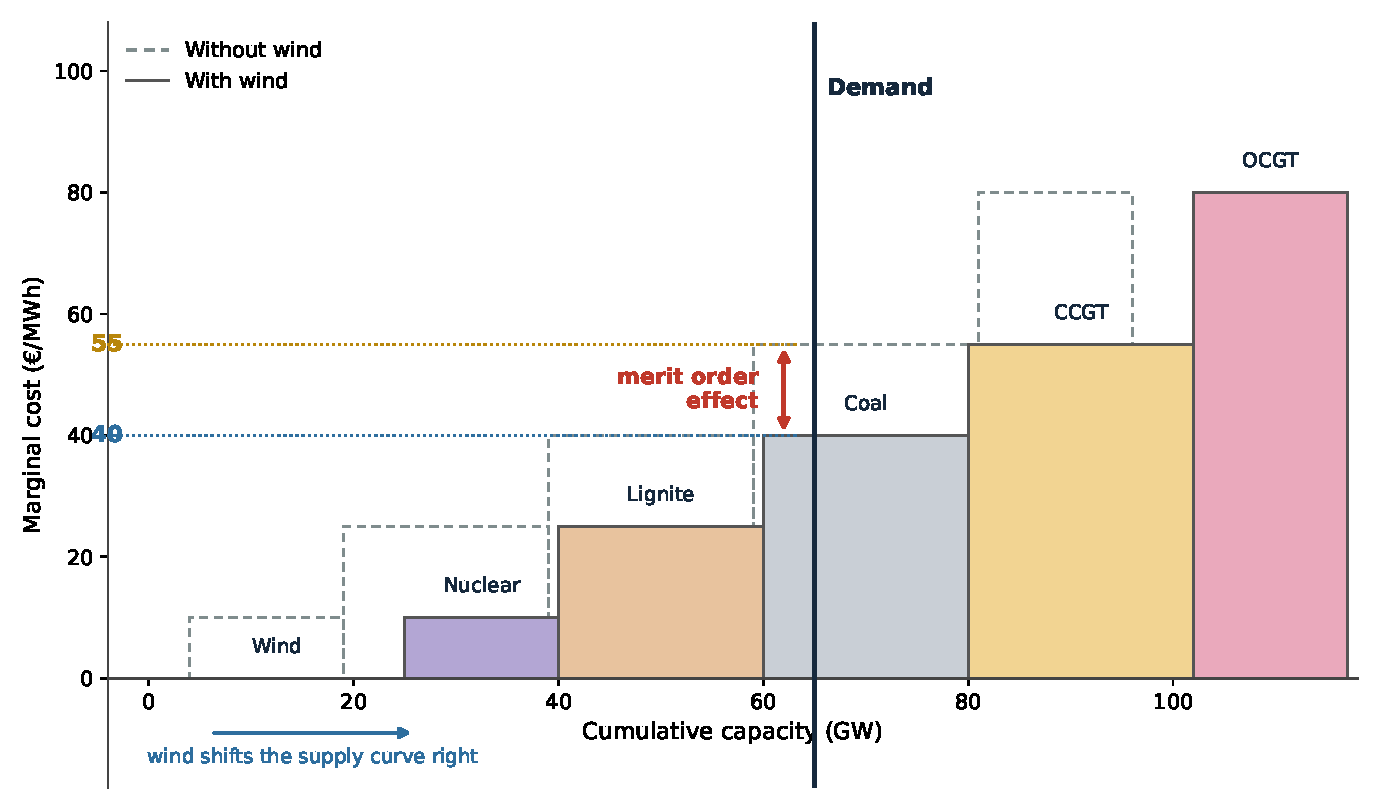
\includegraphics[width=0.82\textwidth]{merit_order_effect}
    \caption{The merit order effect. Wind enters at the bottom of the supply
    curve and shifts it rightward, displacing higher-cost thermal plant and
    reducing the clearing price from 55 to 40~\euro/MWh in this stylised
    example. The depression is deepest in exactly the hours wind generates
    most.}
    \label{fig:merit_order}
\end{figure}

Prices are not formed zone by zone in isolation: the Single Day-Ahead Coupling
mechanism matches orders across participating zones simultaneously, subject to
available cross-zonal transmission \cite{EUPHEMIA2020}. Where transmission is
adequate prices converge and the merit order effect is shared across borders;
where it binds, prices separate and the surplus is trapped \cite{Newbery2018}.
A basin cannot be analysed as a closed system.

Geographic resolution matters as much as mechanism. Europe is divided into
bidding zones, each clearing at one price: Germany prices a single zone despite
substantial internal congestion, a configuration under review whose resolution
would change North Sea wind revenues \cite{Egerer2015, GermanBZSplit2024}, while
the Nordic countries split into eleven zones that let transmission constraints
surface as genuine price areas \cite{Fridolfsson2009}. The three Baltic states
each form their own zone and, since February 2025, are synchronised with the
continental grid rather than the former Soviet system
\cite{BalticSynchronisation2025, ACER2025}.
Figure~\ref{fig:bidding_zones} sets out the zones around both basins with the
interconnectors between them, and groups them by the kind of generation that
usually sets their price, which is the distinction Section~\ref{sec:two_seas}
develops. A zonal structure localises price signals, so cannibalisation
propagates to neighbours only as far as interconnection carries it.

\begin{figure}[!htb]
    \centering
    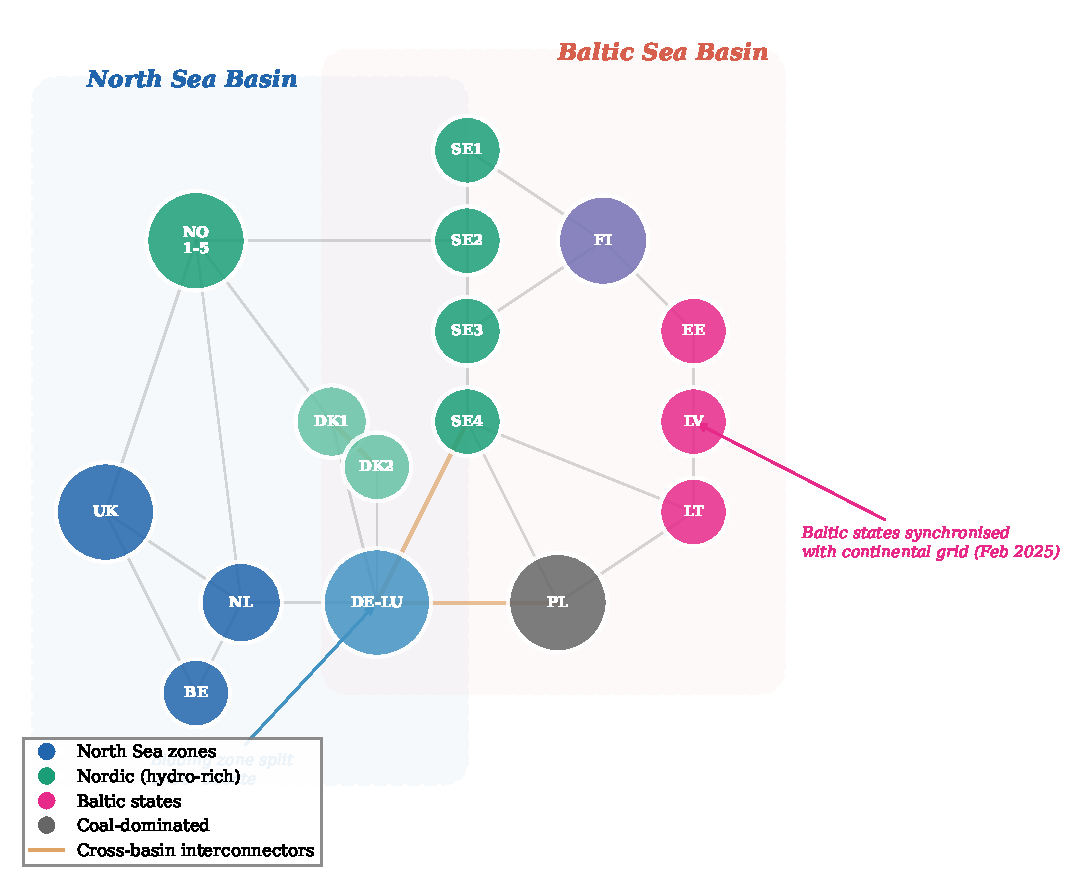
\includegraphics[width=0.78\textwidth]{bidding_zones_map}
    \caption{Bidding zones and the main interconnectors around the North Sea
    and the Baltic. Zones are grouped by the kind of generation that usually
    sets their price: North Sea markets, hydro-rich Nordic markets, the Baltic
    states, which synchronised with the continental grid in February 2025, and
    coal-dominated systems. Interconnectors between the two basins are drawn in
    orange.}
    \label{fig:bidding_zones}
\end{figure}

\subsection{Capture price, cannibalisation and value erosion}\label{sec:value_problem}

\subsubsection{Capture price and capture value}

A baseload plant running continuously earns approximately the time-averaged
wholesale price; a wind farm earns the average price weighted by its own output.
Two measures established by Hirth \cite{Hirth2013} formalise the difference. The
\textit{capture price} is the generation-weighted average spot price received.
Dividing it by the baseload price, the simple time-average of the wholesale
price over the same period, gives the \textit{capture value}:
%
\begin{equation}
    \text{Capture value} = \frac{\text{Capture price}}{\text{Baseload price}}
    = \frac{\sum_{t} p_t \, g_t}{\bar{p} \sum_{t} g_t}
    \label{eq:value_factor}
\end{equation}
%
where $p_t$ is the spot price in hour $t$, $g_t$ the generation, and $\bar{p}$
the time-averaged price. At negligible penetration the ratio sits near unity; as
wind's share grows its own output moves the price in the hours it generates and
the ratio falls. That shortfall is what Hirth \cite{Hirth2015} and Ueckerdt et
al. \cite{Ueckerdt2013} term profile cost, and it is precisely the quantity a
cost-only assessment of where to build omits.

Hirth's early estimates placed the decline at roughly 1.10 at negligible
penetration falling to between 0.50 and 0.80 at a 30\% wind share, the range
separating thermal-dominated systems from hydro-dominated ones
(Figure~\ref{fig:capture_value_decline}) \cite{Hirth2013}. That spread is not
incidental here: most North Sea markets are thermal-heavy, the Baltic rim
borders Scandinavian hydro. Later work at higher penetration has confirmed the
pattern and established that the decline steepens as penetration rises
\cite{Stiewe2025, LopezProl2024, Ember2025, Cevik2022}.

\begin{figure}[!htb]
    \centering
    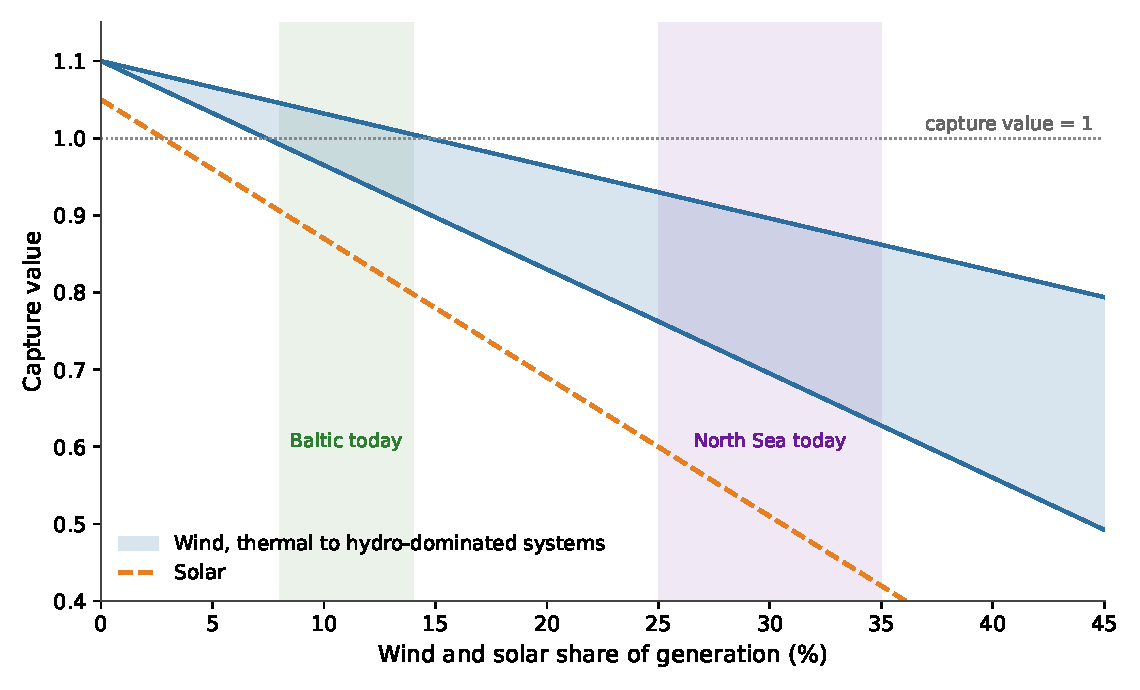
\includegraphics[width=0.7\textwidth]{capture_value_decline}
    \caption[Capture value against wind and solar market share]{Capture value against wind and solar market share,
    synthesised from Hirth \cite{Hirth2013}. The shaded band for wind spans
    thermal-dominated systems (lower bound) to hydro-dominated systems (upper
    bound); the approximate current penetration ranges of the North Sea and
    Baltic markets are indicated.}
    \label{fig:capture_value_decline}
\end{figure}

Figure~\ref{fig:capture_value_traj} shows the divergence directly. Germany's
capture value fell from 0.93 to 0.76 as wind penetration rose from roughly 20\%
to 35\%, while Poland, where wind remained below 18\% of generation and coal
sets the marginal price in most hours, stayed near unity. The Scandinavian
markets sit between the two, buffered by hydro, and the 2021 to 2022 uptick is
the gas crisis lifting wholesale prices faster than capture prices could follow.
The spread between the highest and lowest trajectories widened from five
percentage points in 2015 to twenty by 2024, which is both the severity of the
problem and the reason a basin-level comparison is worth making.

\begin{figure}[!htb]
    \centering
    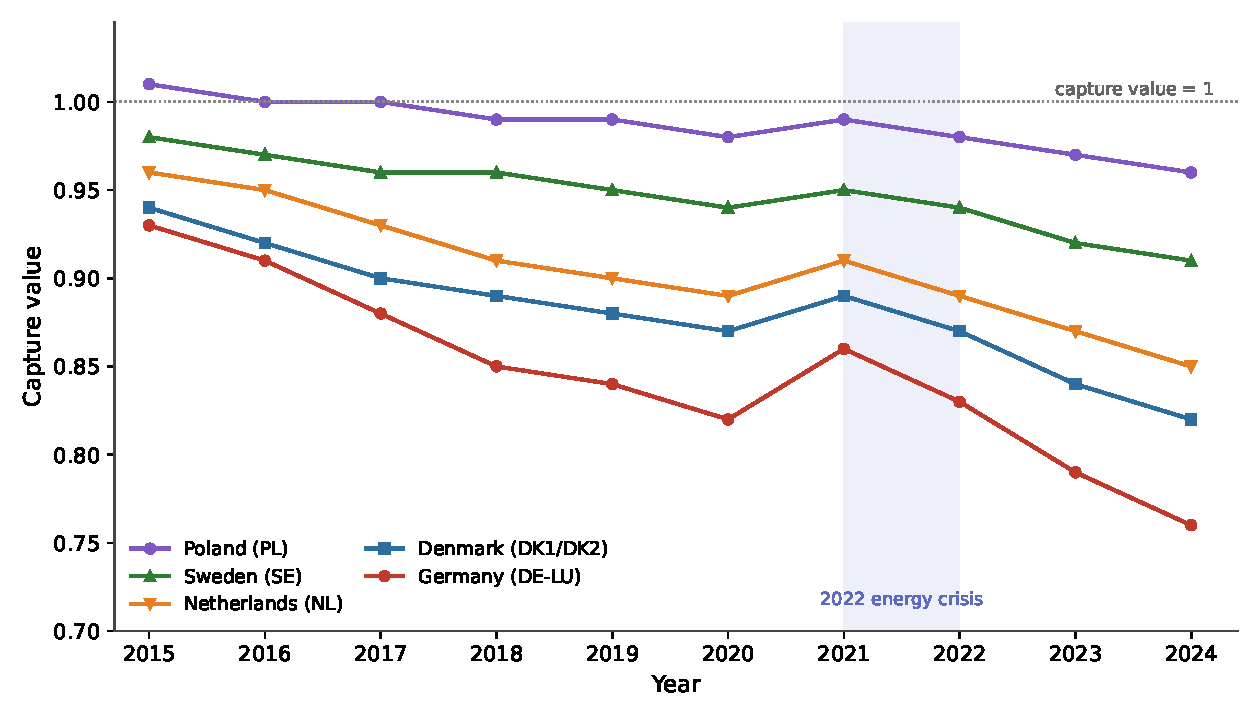
\includegraphics[width=0.86\textwidth]{capture_value_trajectories}
    \caption[Observed offshore capture value, 2015 to 2024]{Observed wind
    capture value for selected European bidding zones, 2015 to 2024, computed as
    the ratio of generation-weighted capture price to baseload price.
    Synthesised from Stiewe et al. \cite{Stiewe2025}, Ember
    \cite{Ember2025, EmberGlobal2024} and ACER market monitoring
    \cite{ACER2023, ACER2025}. The 2021 to 2022 uptick reflects the temporary
    elevation of wholesale prices during the gas crisis.}
    \label{fig:capture_value_traj}
\end{figure}

\subsubsection{Magnitude and measurement}

Estimates of the merit order effect span more than an order of magnitude across
markets, periods and methods \cite{Sensfuss2008, Cludius2014, Lunackova2017},
partly genuine variation and partly the fragility of the identification
assumptions behind them \cite{Wurzburg2013, Clo2015, Kolb2020}. For Baltic
markets published estimates are effectively absent, the pan-European panel of
Cevik and Ninomiya \cite{Cevik2022} being the only work that includes Baltic
zones, and that absence is part of the motivation for this thesis.

Cevik and Ninomiya find that each percentage point of additional renewable share
reduces average wholesale prices by 0.6\%, accelerating at higher penetration
\cite{Cevik2022}. Since wind sells precisely in the hours its own output has
depressed \cite{Hirth2013}, erosion becomes severe past roughly a 20\% wind
share, beyond which Hirth estimates additional wind stops adding system welfare
\cite{HirthOptimal2015}. Offshore is more exposed than onshore: higher and
steadier capacity factors concentrate output in time and correlate it across a
basin, so a sustained blow depresses prices across several coupled zones at once
\cite{Yamujala2026}.

\subsubsection{From price depression to cannibalisation}

The merit order effect describes an instantaneous price depression;
cannibalisation is its cumulative consequence, the revenue earned per
megawatt-hour falling for every existing and prospective asset as capacity
accumulates. Its severity depends on penetration, the spatial correlation of
output, fuel and carbon prices, and the flexibility of the surrounding system
\cite{Hirth2013, Stiewe2025}. Its most visible symptom is the growth of negative
prices, abundant wind meeting inflexible plant that will not curtail and
generators that keep producing because support rewards volume; negative hours
have risen sharply where penetration is highest
\cite{Ember2025, EmberGlobal2024}, masked briefly by the 2022 crisis and
reasserted as gas normalised \cite{Ruhnau2023}. The German fall of
Figure~\ref{fig:capture_value_traj} compounds higher penetration, greater temporal
concentration of offshore output, and the inflexibility of lignite
\cite{Monteil2023, Stiewe2025, Ember2025}.

Whether this is permanent is contested: theory predicts convergence as marginal
generators exit \cite{Antweiler2021, Brown2021}, but European support decouples
investment from market signals and delays that exit \cite{Hirth2013}. The gap is
starkest in small, fast-expanding Baltic markets, where projected revenue losses
reach 15 to 20~\euro/MWh by 2029 against near-zero today
\cite{BalticCannibalisation2024_studies}, too fast for the fleet adjustments
equilibrium arguments assume.

\subsubsection{Cross-border cannibalisation effects}

Most analyses treat each bidding zone as an island. Stiewe et al.
\cite{Stiewe2025} tested that directly, regressing the domestic capture value on
both domestic wind penetration and that of directly interconnected neighbours
across more than 30 zones from 2015 to 2023. A one point rise in domestic
penetration removes 0.61 points of capture value; a simultaneous one point rise
across all neighbours removes a further 0.33, so coordinated European expansion
costs nearly a full point for every point added. The profitability of a Danish
wind farm depends on Dutch, German, Norwegian and Swedish deployment as well as
Danish.

Two features of that identification, the fixed effects absorbing each market's
character and the linear penetration term, are structural limits of statistical
models, and Section~\ref{sec:modelling} returns to what they imply for
projection.

\subsection{Moderators of cannibalisation}\label{sec:mitigation}

The literature so far establishes that capture value falls with penetration
and that the fall propagates across borders, but it largely treats the
surrounding system as fixed. Every mechanism above depends on system
configuration: whether surplus can leave the zone, whether anything absorbs
it, where the fleet is placed, and who is contractually exposed. This section
reviews those four levers.

\subsubsection{Interconnection}

Transmission plays a dual role: capacity exports surplus, relieving domestic
price depression, but imports the depression of high wind next door. Stiewe
et al. find the mitigating effect slightly outweighs the exacerbating one
\cite{Stiewe2025}, and at system scale the benefit is larger, transmission
expansion cutting the total cost of a highly renewable European grid by
roughly 25\% \cite{Schlachtberger2017}.

The scale of planned investment reflects this: more than \euro{}400~billion
of offshore transmission by 2050 under the ENTSO-E Offshore Network
Development Plan \cite{ONDP2024}, with the 70\% cross-zonal trading
requirement pushing markets toward convergence \cite{ACER2023, ACER2025}.
Convergence is double-edged for a generator: surplus exports more easily,
while the importing zone absorbs the corresponding depression.

Congestion is also a revenue stream: whenever a link binds the price differs
across it, and the rent accrues to transmission operators. Joskow and Tirole
\cite{JoskowTirole2005} formalised the awkward consequence, that an investor
relieving the constraint destroys the income justifying the investment, which is
why regulated planning dominates. Article~19 of Regulation (EU) 2019/943
ring-fences those revenues for maintaining or increasing cross-zonal capacity
\cite{EURegulation2019943}, so a congested basin is already earmarking the money
that would relieve it. Neither that accounting nor the question of how much of a
zone's capture value decline is transmission scarcity rather than penetration
has been brought together with capture value analysis, and this thesis
undertakes the decomposition.

\subsubsection{Flexibility and sector coupling}

Storage and conversion attack the same problem in time rather than space.
Hybrid configurations pairing offshore wind with electrolysis absorb surplus
locally \cite{OffshoreHybrids2024}, sector coupling converts it into demand that
would not otherwise exist \cite{Brown2021}, and demand-side flexibility remains
largely unquantified \cite{Hirth2015}. The important observation is negative:
none of these pathways has been integrated into spatial capture value
assessment, so published projections implicitly assume that today's level of
flexibility persists into the future, an assumption that has not been tested at
the scale of a whole basin.

\subsubsection{Spreading the fleet}

The third lever is spatial: if output arrives everywhere at once, placing
capacity where it blows at different times should raise the portfolio's value.
The idea is Markowitz's mean-variance argument \cite{Markowitz1952} applied to
European wind by Roques et al. \cite{Roques2010}. Two things follow that the
literature has not pursued: portfolio treatments optimise the variance of
\textit{generation} while an investor is exposed to the variance of
\textit{revenue}, which market coupling can correlate even where wind is not;
and the mean effect has been neglected, since less severe cannibalisation
arrives as higher average capture value rather than lower volatility.

\subsubsection{Support mechanisms and risk allocation}

The fourth lever is contractual, and it determines not whether value is lost but
who loses it. European governments have moved from guaranteed feed-in tariffs
toward instruments that expose generators to price risk while structuring how it
is shared (Table~\ref{tab:support_mechanisms}).

\begin{table}[!htb]
\centering
\small
\caption{Principal revenue support mechanisms for offshore wind. Market exposure
ranges from none, under a fixed feed-in tariff, to full, under merchant
operation. Two-sided contracts for difference dominate North Sea procurement,
while certificate and premium schemes remain more common around the Baltic.
Basin prevalence is as of 2024.}
\label{tab:support_mechanisms}
\resizebox{\textwidth}{!}{%
\begin{tabular}{l p{7cm} l l}
\toprule
\textbf{Mechanism} & \textbf{Description} & \textbf{Market exposure} & \textbf{Basin prevalence} \\
\midrule
Feed-in tariff & Fixed payment per MWh, independent of market price & None & Legacy, phased out \\
\addlinespace
Two-sided CfD & Strike price agreed; the state pays any shortfall and the generator returns any surplus & Medium & North Sea (UK, NL, DE, PL) \\
\addlinespace
Electricity certificates & Tradable credits per MWh, valued by a separate certificate market & High & Baltic (SE) \\
\addlinespace
Premium schemes & Fixed or sliding premium added to the wholesale price & Medium to high & Baltic states (LT, LV, EE) \\
\addlinespace
Merchant & No direct support; revenue follows wholesale prices entirely & Full & Emerging (NL, DE) \\
\bottomrule
\end{tabular}%
}
\end{table}

The two-sided contract for difference has become dominant: the state pays the
difference when the wholesale price falls below the strike and recovers it
above. The stabilisation lengthens debt tenors and lowers risk margins
\cite{Beiter2024, Dukan2025}, an effect Kitzing et al. argue is structural,
since without it the cost of capital rises enough to negate a decade of
levelised-cost reductions \cite{Kitzing2024}. Premium and certificate schemes
leave operators exposed in exactly the hours cannibalisation is most severe
\cite{Dukan2025}, and the 2024 EU market reform mandated two-sided contracts for
all new supported capacity \cite{EUMarketReform2024}. The geography differs: the
North Sea has converged on mature contract-for-difference frameworks
\cite{WindEurope2025} while the Baltic rim remains a patchwork
\cite{Anatolitis2025}. What this literature does not do is connect contract
design back to the physical decomposition, asking which component of a capture
value decline a given instrument absorbs. That question is taken up here.

\subsection{The North Sea and Baltic Sea as contrasting market environments}\label{sec:two_seas}

\subsubsection{Wind resource and correlation}

European wind is governed by the westerly circulation carrying Atlantic systems
eastward, modulated by weather regimes that swing European mean wind generation
by a factor of two \cite{Grams2017}. Both basins respond to the same patterns,
but partial shielding by the Scandinavian land mass gives the Baltic some
decorrelation from the North Sea.

The resource is unambiguously stronger in the west: mean speeds near
9.75~m\,s$^{-1}$ against 7.5 to 8.0 \cite{Karagali2013}, capacity factors of 40
to 50\% against 35 to 40\% \cite{Solbrekke2022}. The gap narrows once wake
losses are counted, German Bight clusters losing wind speed for up to 70~km
downstream \cite{Schneemann2022} where the sparser Baltic is less affected.

Correlation structure matters as much as resource strength, because simultaneous
output depresses the same hours. Wind power correlation decays exponentially
with distance \cite{Louie2014, Olauson2016} but neither isotropically nor
uniformly: east-west pairs lag as Atlantic fronts propagate eastward, so a North
Sea event precedes its Baltic counterpart by several hours \cite{Malvaldi2017},
and cross-basin correlations sit consistently below within-basin ones
\cite{Olauson2016}. Mehrens et al. \cite{Mehrens2016} estimate a decorrelation
length of about 425~km (Figure~\ref{fig:correlation_decay}); set against the
North Sea's span of roughly 580 by 960~km, farms within a basin are strongly
correlated hourly, so high-generation events are basin-wide. Decay is slower
offshore than onshore \cite{Potisomporn2022} and persists over far greater
distances at weekly aggregation \cite{Hjelmeland2023}.

\begin{figure}[!htb]
    \centering
    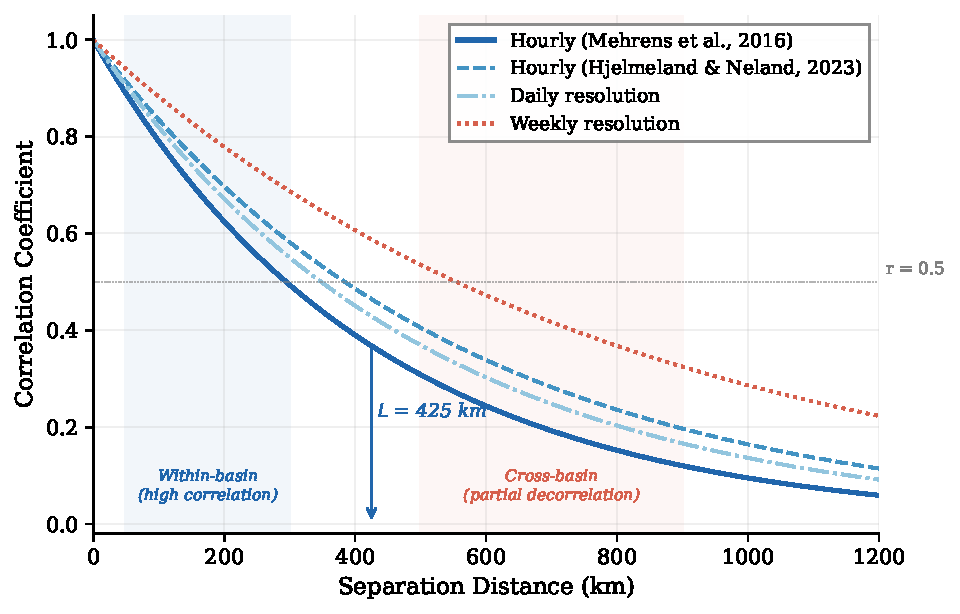
\includegraphics[width=0.72\textwidth]{correlation_decay}
    \caption[Wind power correlation against separation distance]{Wind power correlation against separation distance at different
    temporal resolutions, after Mehrens et al. \cite{Mehrens2016} and
    Hjelmeland and Neland \cite{Hjelmeland2023}. Typical within-basin
    separations (50 to 300~km) sit on the high-correlation shoulder;
    cross-basin separations (500 to 900~km) fall past the decorrelation length
    of about 425~km.}
    \label{fig:correlation_decay}
\end{figure}

Market coupling transmits
price effects across borders, so zones that are physically distant but well
interconnected can show more correlated prices than their wind resources would
suggest. Whether the partial decorrelation of output between the basins survives
into a corresponding decorrelation of capture prices, or whether coupling erodes
that diversification benefit, has not been established, and it bears directly on
whether spreading investment across both basins is a genuine hedge.

\subsubsection{Market structure and the penetration gradient}

The composition of the surrounding fleet sets the slope of the merit order curve
and with it the price response to wind (Figure~\ref{fig:gen_mix}), and four archetypes span the range. Germany, its dispatchable fleet still dominated by
coal, lignite and gas, presents a steep curve in which each increment of wind
produces a large price swing, and its size propagates that volatility to its
neighbours \cite{Ember2025, GermanPrices2023}. Denmark, despite Europe's highest
wind penetration at roughly 55\% of generation, has not seen capture values
collapse as theory predicts, because exceptional interconnection to Nordic hydro
flattens the curve it faces \cite{DanishEnergyAgency2024, Hirth2013}. Sweden,
with hydro near 45\% of production, offers the region's most favourable
environment: at 30\% penetration Hirth estimates wind capture value about
18\% higher in hydro-dominated than thermal-dominated systems \cite{Hirth2013},
wide enough to move a marginal project from loss to viability. Poland sits at
the opposite pole, coal above 60\% of generation \cite{EmberGlobal2024} and
5.9~GW of offshore planned by 2030 \cite{Owczarek2021}, so early projects earn
high capture prices by displacing expensive coal while the programme itself
erodes the conditions that made them attractive. Finland and Estonia are just
entering the same cycle \cite{FinlandOffshoreWind2025, EstoniaOffshoreWind2025}.
Table~\ref{tab:country_archetypes} consolidates the archetypes.

\begin{figure}[!htb]
    \centering
    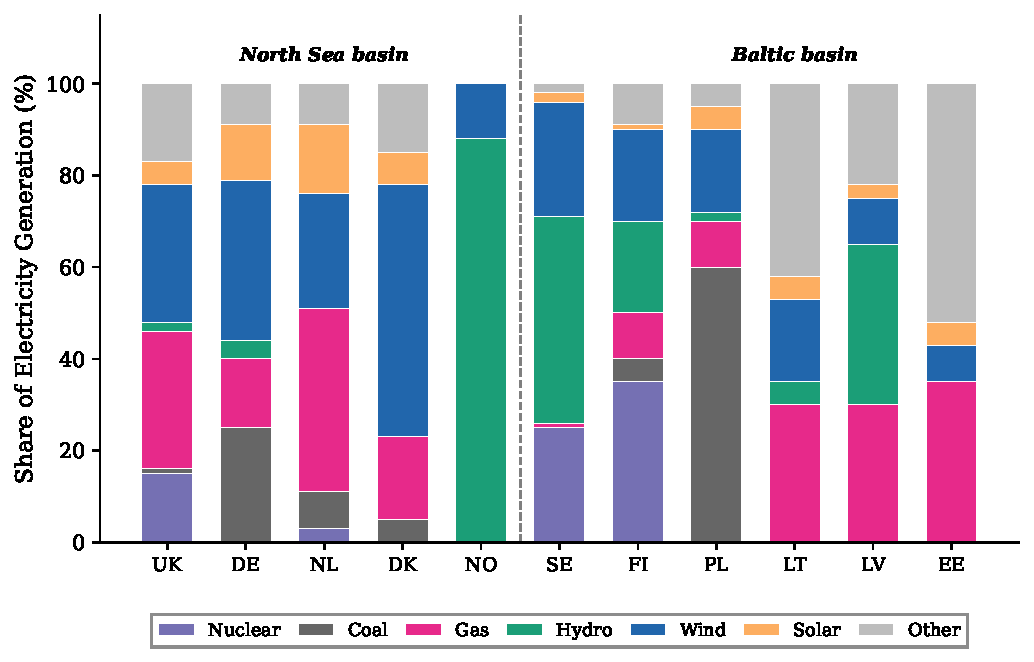
\includegraphics[width=0.9\textwidth]{generation_mix_comparison}
    \caption[Generation mix across the countries bordering the two basins]{Electricity generation mix across the countries bordering the two
    basins, approximate 2024 shares, from Ember \cite{Ember2025} and national
    system operators. Thermal-heavy systems such as Germany and Poland have
    steep merit order curves, in which wind output moves the price sharply.
    Hydro-dominated systems such as Sweden and Norway absorb the same
    variability with little price impact.}
    \label{fig:gen_mix}
\end{figure}

\begin{table}[!htb]
\centering
\small
\caption{Market archetypes around the two basins. Wind penetration and value
factor estimates reflect approximate 2024 values; the final column gives the
dominant revenue support instrument for offshore wind.}
\label{tab:country_archetypes}
\resizebox{\textwidth}{!}{%
\begin{tabular}{l c c l l c c l}
\toprule
\textbf{Country} & \textbf{Basin} & \textbf{Wind (\%)} & \textbf{Dominant gen.} & \textbf{Flexibility} & \textbf{Intercon.} & \textbf{Capture value} & \textbf{Support} \\
\midrule
Germany & NS & $\sim$35 & Gas, coal, wind & Limited; gas peakers & Medium & 0.76--0.85 & Two-sided CfD \\
\addlinespace
Denmark & NS/BS & $\sim$55 & Wind, gas & Nordic hydro (import) & Very high & 0.80--0.90 & CfD (from 2025) \\
\addlinespace
Netherlands & NS & $\sim$25 & Gas, wind & Gas peakers; import & High & 0.85--0.90 & SDE++ tender \\
\addlinespace
UK & NS & $\sim$30 & Gas, wind, nuclear & Gas CCGT; storage & Medium & 0.80--0.85 & CfD (AR rounds) \\
\addlinespace
Sweden & BS & $\sim$25 & Hydro, nuclear, wind & Large hydro reservoirs & High & 0.90--0.95 & Certificates \\
\addlinespace
Finland & BS & $\sim$20 & Nuclear, hydro, wind & Hydro; nuclear baseload & High & 0.90--0.95 & Premium / CfD \\
\addlinespace
Poland & BS & $\sim$18 & Coal, gas & Limited; coal inflexible & Low & 0.95--1.00 & CfD auction \\
\addlinespace
Baltic states & BS & $<$15 & Gas, import, wind & Limited; import-dependent & Medium & $\sim$1.00 & Premium schemes \\
\bottomrule
\end{tabular}%
}
\end{table}

The pattern is striking and, on the conventional reading, paradoxical: every
Baltic market currently records a higher capture value than every North Sea
market, despite uniformly lower interconnection and, in Poland's case, minimal
system flexibility. Penetration is the dominant
predictor of capture value today. Whether that ordering survives as Baltic
capacity scales from single to double-digit gigawatts is the question a
cross-basin comparison exists to answer.

Both basins have committed to expansion on a scale that will settle it: at
least 65~GW of North Sea offshore by 2030 under the Esbjerg Declaration
\cite{Esbjerg2022} and 19.6~GW in the Baltic under Marienborg, a sevenfold
increase \cite{Marienborg2022}, consolidated by ENTSO-E into 146 and 43~GW by
2050 \cite{ONDP2024} against a Baltic technical potential of 93~GW
\cite{Barzehkar2024}. North Sea markets, already at high penetration, face
the steepest marginal declines; Baltic markets begin further back on the
curve. The timing and severity of what follows is a forecasting problem, and
it is to the tools for that problem that the chapter now turns.

\subsection{Models for estimating capture value}\label{sec:modelling}

The question posed in Section~\ref{sec:mitigation}, how much of the value
erosion is removable by design, cannot be answered by any single tool. It
demands four things at once: an hourly generation profile at any point in either
basin, including places where no turbine yet stands; a price for that generation
in the local market, both as it has behaved and as it would behave under a fleet
that does not yet exist; a way to establish that those prices are credible; and a
spatial frame in which locations can be compared on revenue rather than on
energy. Each requirement has its own literature, and each of those literatures stops
short of the others. This section takes them in turn.

\subsubsection{Modelling generation from meteorological data}

A comparison spanning both basins requires one reanalysis product applied
identically to each. Higher-resolution regional products represent coastal
gradients better \cite{Solbrekke2022, Spangehl2021}, but none spans both basins
at the hourly resolution capture value requires. ERA5, at 0.25\textdegree{} and
hourly from 1940, is the only product that does, and it has been validated
against tall towers \cite{Staffell2016, Ramon2019} and North Sea platforms at
$r = 0.85$ to $0.93$ \cite{Bot2024}. Its known weakness is that it
underestimates strong offshore winds, by roughly 15\,\% at 15~m\,s$^{-1}$
\cite{Gandoin2024}, which the cubic relationship between speed and power
amplifies into an error in capacity factor.

Converting wind fields into power follows the standard procedure of Staffell and
Pfenninger \cite{Staffell2016}, now implemented in open tools such as atlite
\cite{Hofmann2021}. A bias correction against fleet data is not optional in that
procedure, since uncorrected reanalysis understates offshore capacity factors by
12 to 15\,\%.

\subsubsection{Models of electricity prices}

Electricity prices are among the hardest commodities to model, combining extreme
volatility, seasonality on several timescales, and mean reversion punctuated by
spikes \cite{Weron2014}. Two of Weron's five families matter here, and the
distinction organises this thesis: statistical models estimate the relationship
between wind and price from what markets have done, and system models rebuild it
from what the system is made of. Behind both sits a general trade-off
\cite{Pfenninger2014, Ringkjob2018}: tools with fine spatial resolution simplify
temporal dynamics, and tools with rich temporal detail aggregate space.
Table~\ref{tab:modelling_comparison} places the principal tools against the
requirements above. Zeyringer et al. \cite{Zeyringer2018} show what the gap
costs: designs that neglect the coincidence of high wind and low prices
overestimate how much capacity is worth building.

\begin{table}[!htb]
\centering
\small
\caption{Principal modelling tools against the requirements of this thesis.
Each covers one dimension of the problem, resource, price, network, or space,
and stops short of the others.}
\label{tab:modelling_comparison}
\resizebox{\textwidth}{!}{%
\begin{tabular}{l l c c p{4.3cm} p{4.3cm}}
\toprule
\textbf{Tool} & \textbf{Type} & \textbf{Spatial} & \textbf{Temporal} &
\textbf{Key strength} & \textbf{Missing dimension} \\
\midrule
atlite \cite{Hofmann2021} & Resource conversion & 0.05--0.25$^{\circ}$ & Hourly &
Open; flexible weather cutouts & No market or revenue component \\
\addlinespace
Renewables.ninja \cite{Staffell2016} & Resource conversion & Site & Hourly &
Bias-corrected; validated globally & No market or revenue component \\
\addlinespace
PyPSA-Eur \cite{Horsch2018} & System optimisation & Nodal & Hourly &
Full European network; open & Shadow prices rather than observed prices \\
\addlinespace
Balmorel \cite{Wiese2018} & System optimisation & Zonal (Nordic--Baltic) & Hourly &
Regional hydro coupling; open & Regional scope; same price caveat \\
\addlinespace
EuroMod \cite{Mendes2024} & Dispatch / market & Zonal (27) & Hourly &
Realistic price volatility & Proprietary data; tied to calibration period \\
\addlinespace
PLEXOS \cite{PLEXOS2024} & Unit commitment & Nodal/zonal & Sub-hourly &
Industry standard; generator detail & Proprietary and costly \\
\addlinespace
Stiewe et al. \cite{Stiewe2025} & Panel regression & Zonal (30+) & Annual &
Cross-border spillovers & Fixed effects absorb the why; no map \\
\addlinespace
Bosch et al. \cite{Bosch2017, Bosch2018, Bosch2019} & GIS spatial & 0.05$^{\circ}$ &
32 slices/yr & Depth, distance, LCOE & No market value or revenue \\
\bottomrule
\end{tabular}%
}
\end{table}

\textbf{Statistical models} estimate the relationship from observed data. Hirth
\cite{Hirth2013} combined meta-regression with dispatch modelling to estimate the
slope of capture value against penetration. Stiewe et al. \cite{Stiewe2025}
extended this to a panel across more than thirty zones,
%
\begin{equation}
    VF_{i,t} = \alpha_i + \beta_1\, WP_{i,t} + \beta_2\,
    \overline{WP}_{N(i),t} + \gamma \mathbf{X}_{i,t} + \varepsilon_{i,t},
    \label{eq:stiewe_model}
\end{equation}
%
where $VF_{i,t}$ is the wind capture value in zone $i$, $WP_{i,t}$ is domestic
wind penetration, $\overline{WP}_{N(i),t}$ is the capacity-weighted penetration
of directly interconnected neighbours, and $\alpha_i$ is a zone fixed effect.
That fixed effect is where the explanatory limit sits: everything that makes one
market different from another is absorbed into a single intercept. Maciejowska
\cite{Maciejowska2020} showed that wind compresses the upper tail of the price
distribution more than it shifts the mean, which is why capture prices fall
faster than average prices, and machine-learning variants have improved
short-term forecasting accuracy over linear specifications
\cite{Lago2021, Marcjasz2023}.

The defining constraint of this family is structural: a model fitted over a
range of conditions describes that range. Tree ensembles, the strongest
performers in recent comparisons \cite{Lago2021}, are piecewise constant by
construction, so beyond the training data no splits exist and the prediction
stops changing. A linear specification will extend beyond its data, but only by
asserting that a slope estimated at penetrations of 10 to 35\,\% still holds at
60\,\%, which is precisely where the evidence says the relationship steepens
\cite{Cevik2022, LopezProl2024}.

\textbf{System models} construct the price instead of fitting it. A
cost-minimising dispatch and investment program returns the shadow price of the
energy balance at each node, which under marginal-cost pricing is the wholesale
price. Green and Vasilakos \cite{GreenVasilakos2011} applied this to the British
market early, finding that large-scale offshore deployment lowers wholesale
prices and with them the revenue of the deployers themselves. PyPSA-Eur
\cite{Horsch2018, PyPSA2024} provides an open implementation with the full
European transmission network at nodal resolution, since extended globally
\cite{PyPSAEarth2024}. Because such a model re-derives the merit order for any
system state, it can price configurations that have never existed, which is what
a 2040 scenario requires.

Its errors are equally structural and run in a known direction. The shadow price
excludes mark-ups, strategic bidding and scarcity rents \cite{Mays2023}. Without
unit commitment the model cannot bid below zero, so it cannot reproduce the
negative prices that are cannibalisation's sharpest symptom \cite{Ruhnau2023}.
Perfect foresight lets storage, and Nordic hydro in particular, absorb surplus at
exactly the right moment. Clustering the network hides congestion inside each
node. Every one of these approximations raises capture value, and each is
largest in small, hydro-adjacent, well-interconnected zones. Commercial tools
relax some of them through non-convex generator constraints
\cite{PLEXOS2024, Mendes2024} but require proprietary plant data, and the Nordic
and Baltic region has its own open lineage in Balmorel \cite{Wiese2018}, which
shares the same approximations. One boundary applies to both families: adding
neighbouring countries' generation and prices measurably reduces day-ahead
forecasting error \cite{VanDerHeijden2021}, so no single-zone model of either
kind sees the whole mechanism.

\subsubsection{Comparison of the two model families}

A statistical model is accurate
where observations are dense, and beyond them it stops responding to its inputs.
A system model can price any future, but it simplifies the market it rebuilds,
and the error that follows is consistently in the same direction. Neither
limitation can be removed by improving a model within its own family.

No study compares them directly: where both estimates of the same quantity
exist, the literature offers no way to decide which to believe, no test for the
point at which one should replace the other, and no comparison with observation
that would reveal the consistent error of the one and the flat response of the
other. Supplying that comparison is one contribution of this thesis.

The tools for making it are standard and have simply not been applied to this
question. They cover the choice of error measure \cite{HyndmanKoehler2006}, the
separation of a consistent offset from other kinds of error \cite{Theil1966},
testing whether a difference in accuracy is real \cite{DieboldMariano1995}, and
holding out whole locations or whole periods rather than individual observations
when data are structured in space and time \cite{Roberts2017}.
Section~\ref{sec:gap_method} sets out how each is used here. What matters for the
argument is that the two families fail differently, so a comparison reporting
only an average error would conceal exactly the difference that decides which
model carries a projection.

\subsubsection{LCOE and its extensions}
\label{sec:vlcoe_lit}

The most developed spatial framework is the progression by Bosch, Staffell
and Hawkes \cite{Bosch2017, Bosch2018, Bosch2019}, which moved from gridded
capacity factors, to offshore depth and distance constraints, to spatially
resolved levelised cost, and was later extended globally \cite{Chu2020}, all
on open bathymetry and resource data \cite{GEBCO2014, GlobalWindAtlas}.
What these frameworks optimise is the levelised cost of energy (LCOE), the
lifetime cost of a project per megawatt-hour produced, which is the standard
basis for comparing technologies and sites \cite{IRENA2025Costs, BCG2025}.

These frameworks characterise cost comprehensively and revenue not at all. A
site with low levelised cost may still return poorly if it sells into a market
where cannibalisation has driven capture prices below that cost.

A parallel literature has long argued that levelised cost is the wrong
comparator. Ueckerdt et al. \cite{Ueckerdt2013} decomposed integration cost into
profile, balancing and grid components, of which profile cost is exactly the
capture value shortfall of Section~\ref{sec:value_problem}; Hirth
\cite{Hirth2015} made the same argument through market value; the International
Energy Agency operationalised it as the value-adjusted levelised cost of
electricity \cite{IEAValcoe2018}; and Joskow \cite{Joskow2019} had earlier
objected that comparing levelised costs across technologies with different
output profiles is economically meaningless.

The gap is that the two literatures have been kept apart. Value-adjusted metrics
are computed for a technology within a system; spatial frameworks for a location
within a map. Nobody has computed a value-adjusted cost \textit{per location},
which is what an investor choosing between a Polish and a German site needs, and
which is necessary before asking whether a ranking of sites by cost survives the
addition of value.

This thesis closes that gap with one derived metric. A merchant farm breaks
even when the price it captures covers its levelised cost; its captured price
is $\bar p\,\mathrm{CV}$ (Equation~\ref{eq:value_factor}), so the average
wholesale price a site needs is
%
\begin{equation}
  \mathrm{vLCOE} \;=\; \frac{\mathrm{LCOE}}{\mathrm{CV}},
  \label{eq:vlcoe}
\end{equation}
%
the \emph{value-adjusted LCOE}. Where the IEA's VALCOE adjusts a technology's
cost additively within one system \cite{IEAValcoe2018}, this metric is
multiplicative, carries the measured capture value directly, and is computed per
location, so it can be mapped. Because capture value sits in the denominator it
can rise even as the raw LCOE falls, whenever cannibalisation erodes value
faster than learning cuts cost.

\subsection{Research gaps and questions}\label{sec:research_gap}

Four gaps follow from the review.

\textbf{No systematic cross-basin comparison of capture value.} Capture values
have been measured within national markets and across a European panel
\cite{Stiewe2025}, but no study compares them across the full set of bidding
zones surrounding both basins under a consistent method, and merit order
estimates for Baltic markets are effectively absent \cite{Cevik2022}.

\textbf{Cannibalisation is treated as a property of penetration rather than of
system design.} The decline is well documented and interconnection and
flexibility are known to moderate it
\cite{Stiewe2025, Schlachtberger2017, OffshoreHybrids2024}, but the literature
does not decompose a decline into the portion a different system configuration
would remove and the portion that is structural. Without that split, a capture
value figure cannot distinguish a transmission problem from an oversupply
problem, and the policy implications of the two are opposite.

\textbf{Market value is absent from spatial assessment, and support design from
both.} GIS frameworks rank sites on cost while ignoring revenue
\cite{Bosch2017, Bosch2018, Bosch2019}, and the contract-design literature
\cite{Beiter2024, Kitzing2024, Dukan2025, Anatolitis2025} treats revenue risk as
a financing question rather than asking which physical component of a value
decline a given instrument absorbs.

\textbf{No method both measures and projects.} Statistical models are accurate
in sample and cannot extrapolate beyond their support; system models project
freely and carry structural bias. The literature offers no validated procedure
for combining them or for establishing at which point one should replace the other.

These gaps motivate three research questions.

\begin{enumerate}
    \item How does offshore wind capture value in the enclosed Baltic compare
    with the open North Sea today, and how does it evolve under the committed
    buildout to 2030 and 2040?
    \item Which market mechanisms determine the rate of value erosion, do they
    differ between an enclosed and an open basin, and how much of the erosion is
    removable by system design rather than inherent to the resource?
    \item Can a model trained on historical observation project these futures, or
    is a system model required, and how should the two be combined and validated
    against each other?
\end{enumerate}

The third question is the one on which the other two depend, since every
projected number in this thesis comes from one model or the other, and it is the
one the literature leaves most open. This thesis builds one model of
each kind, a statistical model fitted to eight years of observed prices and a
system model that rebuilds the market from physics and cost, and sets them side
by side. Somewhere the two will disagree, and the practical decision is which of
them produces the 2040 numbers this thesis reports. Section~\ref{sec:confrontation}
sets out how that decision is made from measurement rather than by inspection.

Answering the first question is of limited use if the answer stops at a ratio.
A capture value only changes a decision once it is priced, so this thesis also
carries the projected values onto the map and folds them into cost, giving the
average wholesale price each location must earn to break even. That step turns
the measured erosion into the question an investor faces, which is
where to build and whether the cheapest site is still the best one.

Answering these requires four objectives, running from the apparatus outward to
the decisions it informs.

\begin{enumerate}
    \item \textit{Build and validate the two models.} Construct a virtual wind
    farm from reanalysis and validate it against metered generation; fit a
    capture value model carrying market characteristics as explicit features
    rather than fixed effects, scored by leaving whole farms out; configure an
    open system model of both basins under official capacity trajectories; and
    confront both against observation where reality can arbitrate.

    \item \textit{Measure and project capture value across both basins.}
    Establish where each bidding zone stands today and how it evolves to 2030
    and 2040 under the committed buildout.

    \item \textit{Decompose the erosion into removable and structural parts.}
    Separate what an unconstrained network or a flexible demand side would
    remove from what the buildout imposes regardless, and identify who bears
    each part once support contracts are accounted for.

    \item \textit{Map the value-adjusted cost of energy and test whether capture value
    changes where to build.} Carry the validated capture values onto the map
    alongside resource, water depth and distance to shore, and fold them into
    cost to give a \textit{value-adjusted levelised cost of energy}, the average
    wholesale price a site must earn to break even, computed per location rather
    than per technology. Then compare the ranking of candidate sites by cost
    alone against the ranking once value is included. If the rankings agree a
    cost-only screen is sufficient; if they diverge, site selection has been
    made on an incomplete criterion, and the divergence grows over the period
    across which projects are financed.

    \end{enumerate}

The remainder of this thesis pursues these objectives using open data
throughout, so that every step from raw download to final figure can be
inspected and re-run.

% ============================================================================
% Chapter 3 · Methodology
% Style: no em dashes. Reasons before mechanics, plainly. One experiment, two
% instruments, one comparison against observation. Each concept introduced before use.
% ============================================================================

\section{Methodology}\label{sec:methodology}

\subsection{Rationale for a two-model approach}
\label{sec:design}

The rationale for building two models is a single comparison: one model is
constructed from first principles and the other learns from past trends, and
setting both against observed prices establishes which is better suited to
projecting a future that has not been observed. Furthermore, seeing if one is better suited for short term vs long term projection. More details on the logic flow of both models can be found in figure \ref{fig:architecture} and table \ref{tab:models}.

\begin{figure}[H]
    \centering
    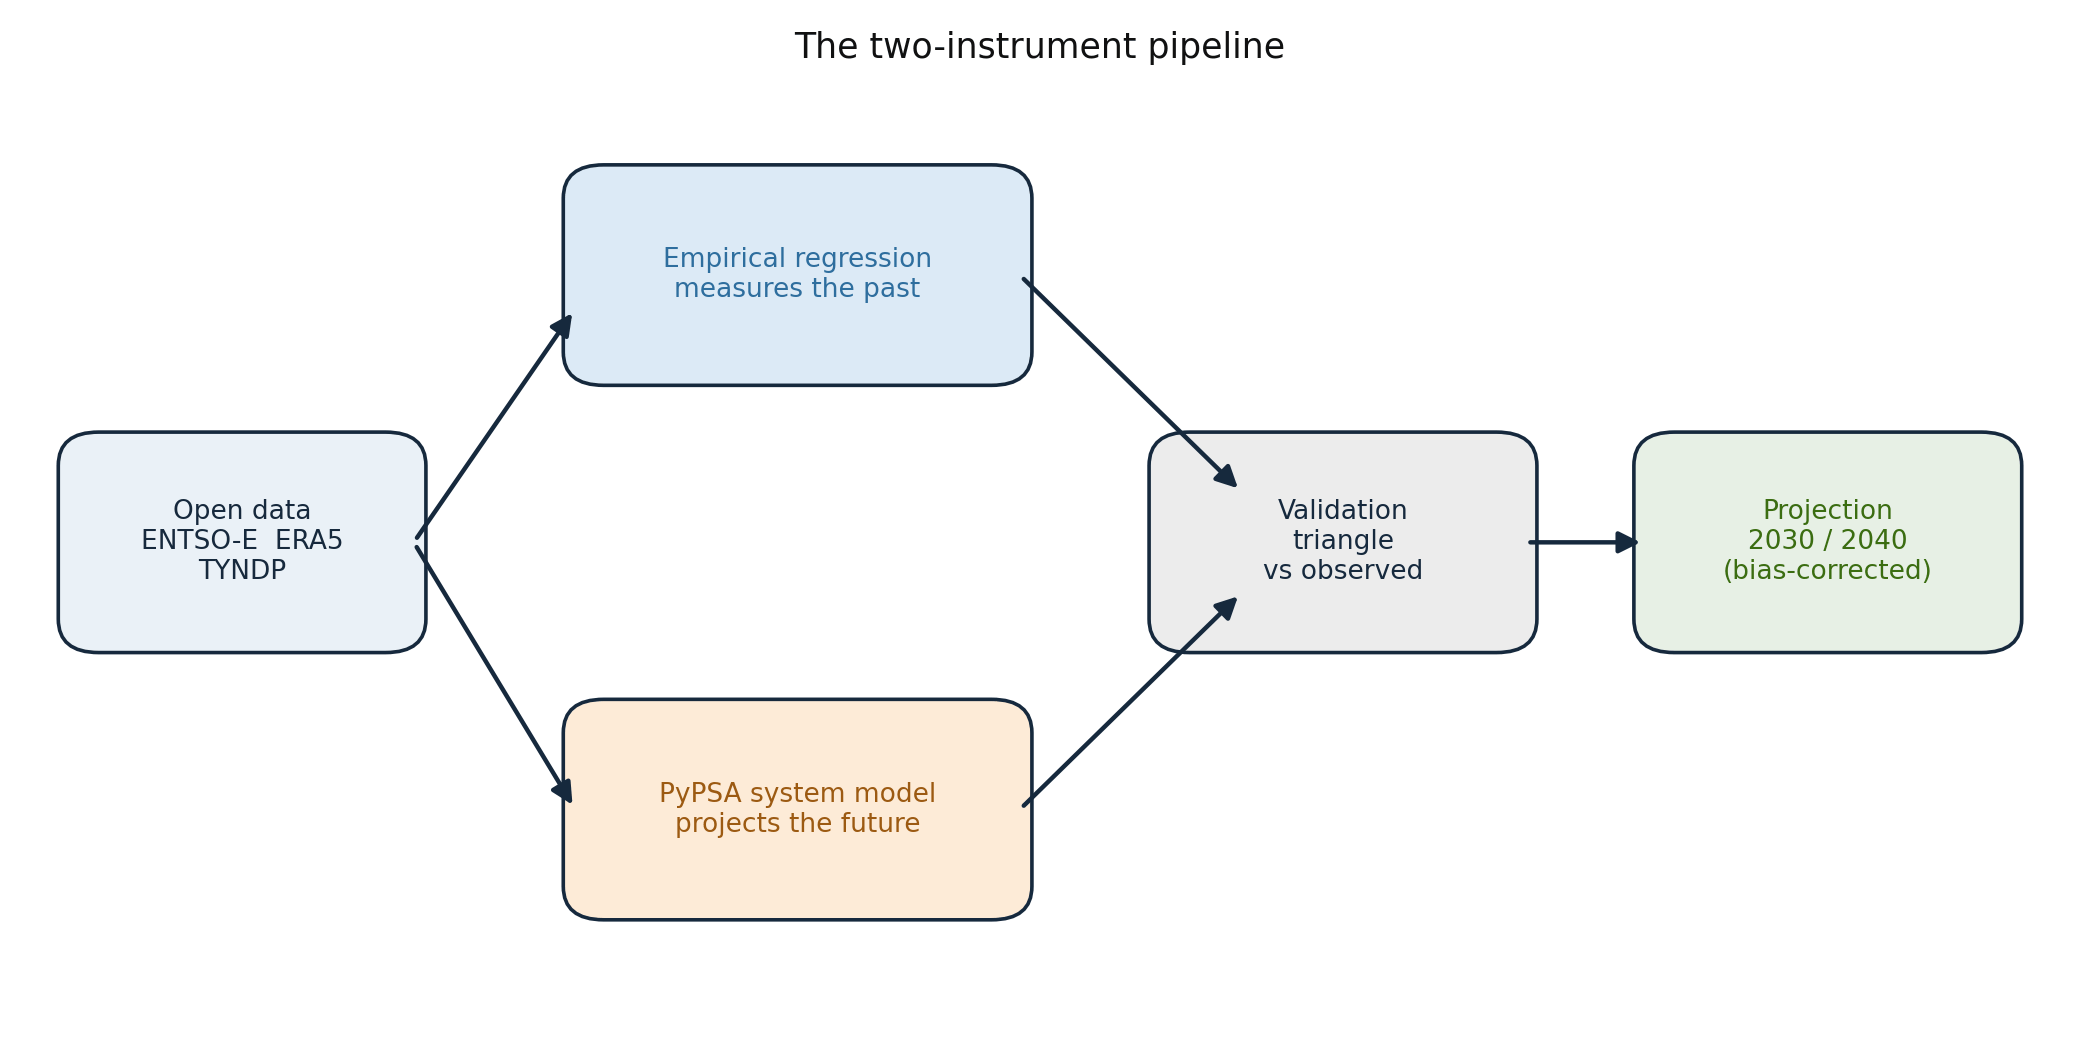
\includegraphics[width=0.95\textwidth]{architecture}
    \caption{The design of the thesis. Shared data feed the two models, both
    are compared against observed capture values, and the comparison decides
    which model is used for what.}
    \label{fig:architecture}
\end{figure}

\begin{table}[!htb]
\centering\small
\caption{How the two models are built, what they produce, and what each is used
for.}
\label{tab:models}
\begin{tabular}{p{2.7cm} p{5.6cm} p{5.6cm}}
\toprule
 & \textbf{Regression model} & \textbf{System model} \\
\midrule
Algorithm & Gradient-boosted trees (XGBoost) & Linear optimisation in PyPSA-Eur
(Gurobi) \\
\addlinespace
Built from & Seven market conditions, measured monthly for 31 farms from 2017 to
2024, giving 2{,}706 observations & The transmission grid, generation fleets,
ERA5 weather and TYNDP scenarios, solved hourly across thirty nodes \\
\addlinespace
Produces & Monthly capture value for each farm & Hourly prices and generation in
every zone, and annual capture value per zone \\
\addlinespace
Compared against & Observed capture value, with whole farms held out of the
fitting & Observed capture value in each zone and year \\
\addlinespace
Used for & Measuring the present and explaining the mechanism & Projecting 2030
and 2040, with its measured error subtracted \\
\bottomrule
\end{tabular}
\end{table}

\subsection{The use of capture value}
\label{sec:currency}

The regression
model applies it monthly to each farm, using day-ahead prices. The system model
applies it annually to each zone, using its own modelled prices. The comparison
of Section~\ref{sec:triangle} applies it to both against observation. In every
case it is calculated only over the hours for which both a price and a
generation figure exist, which is what makes the three sets of numbers
comparable. Denmark is treated as two zones throughout, DK1 and DK2.

One feature of the definition matters for what follows. Capture value depends on
the prices in a zone, weighted by when a farm generates. Prices are observed for
every zone in the study, and generation comes from the virtual wind farm of
Section~\ref{sec:vwf}, so a capture value can be measured for any zone with
observed prices, whether or not offshore wind operates there.

The regression model uses this to train on all seven enclosed Baltic zones
instead of the one zone with operating offshore wind. It weights prices that
have already occurred by a wind profile that has been validated against metered
output, so the only unobserved element is the farm itself. The projection in
Chapter 4 asks more than this, since it prices farms in markets that do not yet
exist.

\subsection{Data sources}\label{sec:data}

\subsubsection{Market data}\label{sec:market_data}

All market data come from the ENTSO-E Transparency Platform and cover 2017 to
2024. They comprise day-ahead prices for 22 bidding zones, hourly load, hourly
generation by technology, flows across 28 borders, and the yearly capacity of
each border. Everything is hourly and in UTC, and prices are resolved by bidding
zone rather than by country, so DK1, DK2 and SE4 are separate.

The platform under-reports Dutch renewable generation, which is therefore
rescaled to match physical capacity factors while keeping its hourly shape
\cite{Jacquet2024}, and British day-ahead prices cease publication after
Brexit, so the three British farms contribute only up to 2020. No other
corrections are applied to the market data.

\subsubsection{Meteorological and wind farm data}\label{sec:farm_data}

The study covers 31 offshore wind farms, sixteen in the North Sea and fifteen in
the Baltic, including sites that are operating, under construction and planned.
The operating farms are the ones whose modelled generation can be checked
against metered output, and they are used for validation. Every site in a zone
with observed prices is used to fit the regression model, whether it is
operating or not (Section~\ref{sec:fitting}).

A farm belongs to the sea its foundations stand in. DK2 and SE4 are part of the
Nordic synchronous area, but their farms stand in the western Baltic, experience
Baltic weather, and sell into the same enclosed market as the Polish and
Baltic-state fleets, so they are treated in this work as Baltic.

Within that geography the analysis uses four groups, kept the same throughout.
The open \textbf{North Sea} is the reference: Germany, the Netherlands, Belgium,
DK1 and France. The \textbf{under-built} Baltic is Poland, Estonia, Latvia and
Lithuania, which have very little offshore wind built so far. The
\textbf{built-out} Baltic is DK2 and SE4, which already have offshore wind in
operation. \textbf{Finland} is kept separate, because its low capture value
comes from nuclear generation holding prices down rather than from wind. The
groups are chosen so that the built-out zones show today what the under-built
ones are heading towards.

Hourly wind speeds at 10 and 100 metres come from ERA5, the fifth-generation
reanalysis of the European Centre for Medium-Range Weather Forecasts, taken at
each farm's nearest 0.25 degree grid cell. A reanalysis is a modern weather
model re-run over the past and combined with every available observation, and it
is the standard source of wind data for energy studies. ERA5 is known to
underestimate the strongest offshore winds \cite{Gandoin2024}. These speeds are left uncorrected, because the power-curve adjustment of
Section~\ref{sec:vwf} corrects the average level only, and the validation
reported there tests whether the resulting output is nonetheless accurate.

\subsubsection{Scenario data}\label{sec:scenario_data}

Future capacities, demand, fuel and carbon prices and battery fleets come from
the 2024 Ten-Year Network Development Plan, the official scenario framework of
the European transmission system operators \cite{TYNDP2024}. They are extracted
once into a single set of per-country tables, which both models then use. Because these tables cover renewable technologies only, the thermal capacity
they omit, and the corrections that omission requires, are set out in
Section~\ref{sec:projection}.

\subsection{The regression model}\label{sec:empirical}

\subsubsection{Virtual wind farm model}\label{sec:vwf}

Most of the farms in the study are not yet built, so generation is modelled for
every site, including those already operating. The method follows Staffell and
Pfenninger \cite{Staffell2016} as adapted by Jacquet \cite{Jacquet2024}, in
three steps.

\begin{enumerate}
    \item \textbf{Height extrapolation.} ERA5 gives wind speed at 10 and 100
    metres, and the IEA 15~MW reference turbine used has a hub height of
    150 metres \cite{Gaertner2020}. Speed is carried up to that height by
    fitting a logarithmic profile through the two known levels,
    %
    \begin{equation}
        u(z) = u_{\mathrm{ref}}\,\frac{\ln(z/z_0)}{\ln(z_{\mathrm{ref}}/z_0)},
        \label{eq:log_wind}
    \end{equation}
    %
    where $u(z)$ is the speed at height $z$, $z_{\mathrm{ref}}$ is a height at
    which the speed is known, and the surface roughness $z_0$ is solved from the
    10 and 100 metre pair. This is the standard description of how friction at
    the sea surface slows the wind near it and lets speed increase with height.

    \item \textbf{Power conversion.} Speed is turned into power using the
    turbine's power curve, which rises steeply between the cut-in speed of
    3~m\,s$^{-1}$ and the rated speed near 10.6~m\,s$^{-1}$, then stays flat up
    to the cut-out speed of 25~m\,s$^{-1}$. Output is set to zero outside that
    range, so neither calm nor storm hours produce anything.

    \item \textbf{Fleet adjustments.} Two corrections are applied, both
    calibrated by Hayes et al.\ on metered European farms \cite{Hayes2021}. The
    curve is smoothed ($\sigma = 1.17$~m\,s$^{-1}$), because the turbines across
    a single farm do not all meet the same wind speed, and it is shifted towards
    higher speeds ($w_0 = 0.71$~m\,s$^{-1}$) to account for wake losses and for
    the ERA5 bias noted above (Figure~\ref{fig:power_curve}).
\end{enumerate}

\begin{figure}[!htb]
    \centering
    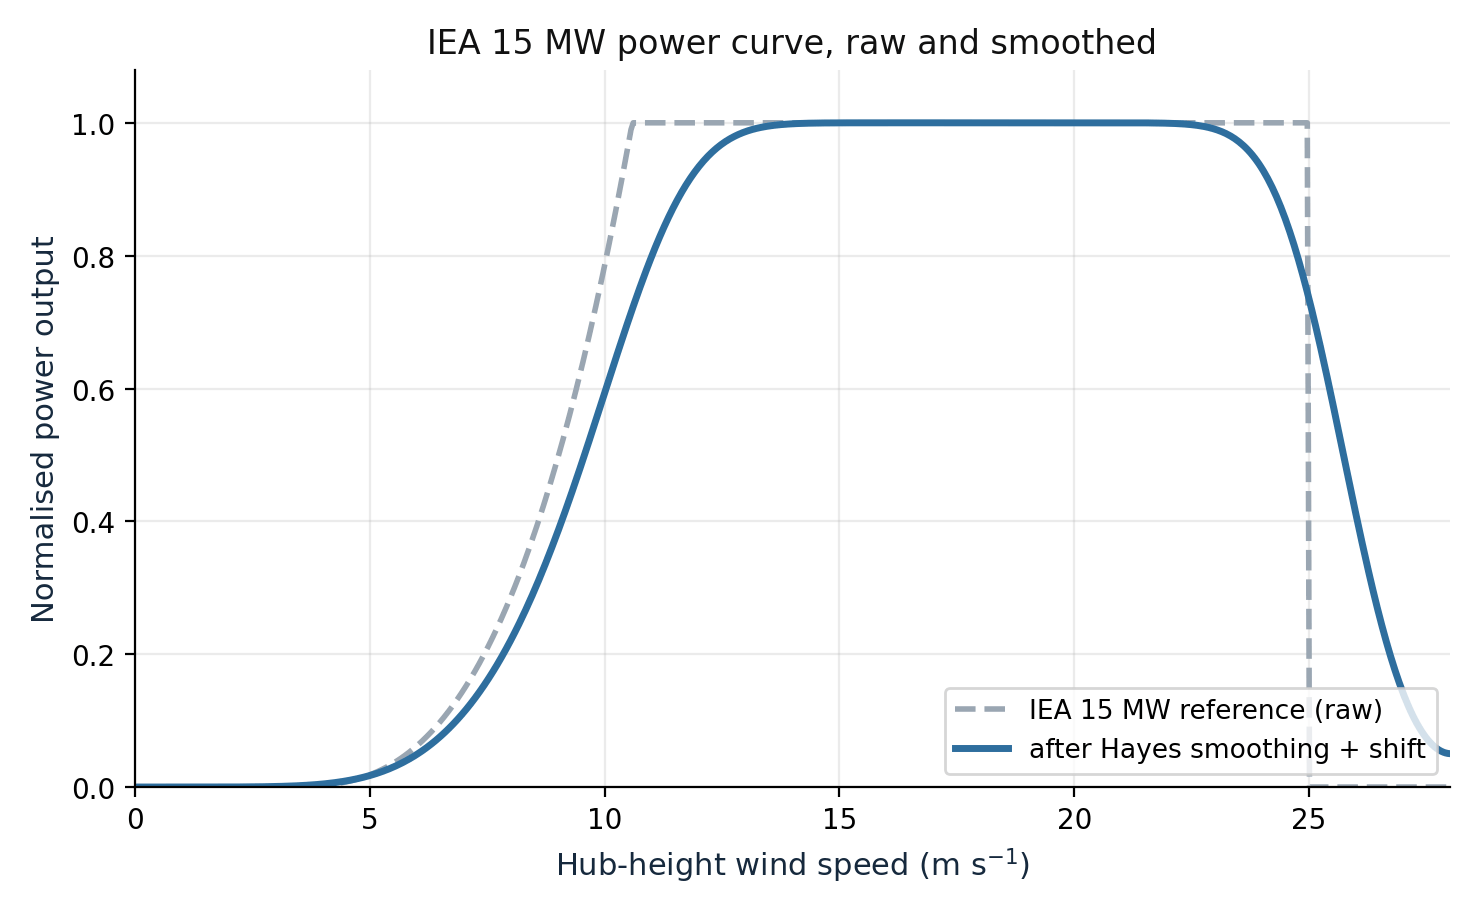
\includegraphics[width=0.62\textwidth]{power_curve}
    \caption{The IEA 15~MW reference power curve before and after the two
    adjustments, used to convert wind speed at hub height into output. Smoothing
    $\sigma=1.17$~m\,s$^{-1}$, shift $w_0=0.71$~m\,s$^{-1}$.}
    \label{fig:power_curve}
\end{figure}

The modelled generation is then checked against metered output. Aggregated to
zone level, the modelled farms reach a median hourly correlation of 0.88 with
the generation ENTSO-E reports, and 0.95 monthly, across five zones and three
years (Figure~\ref{fig:vwf_vs_observed}).

\begin{figure}[!htb]
    \centering
    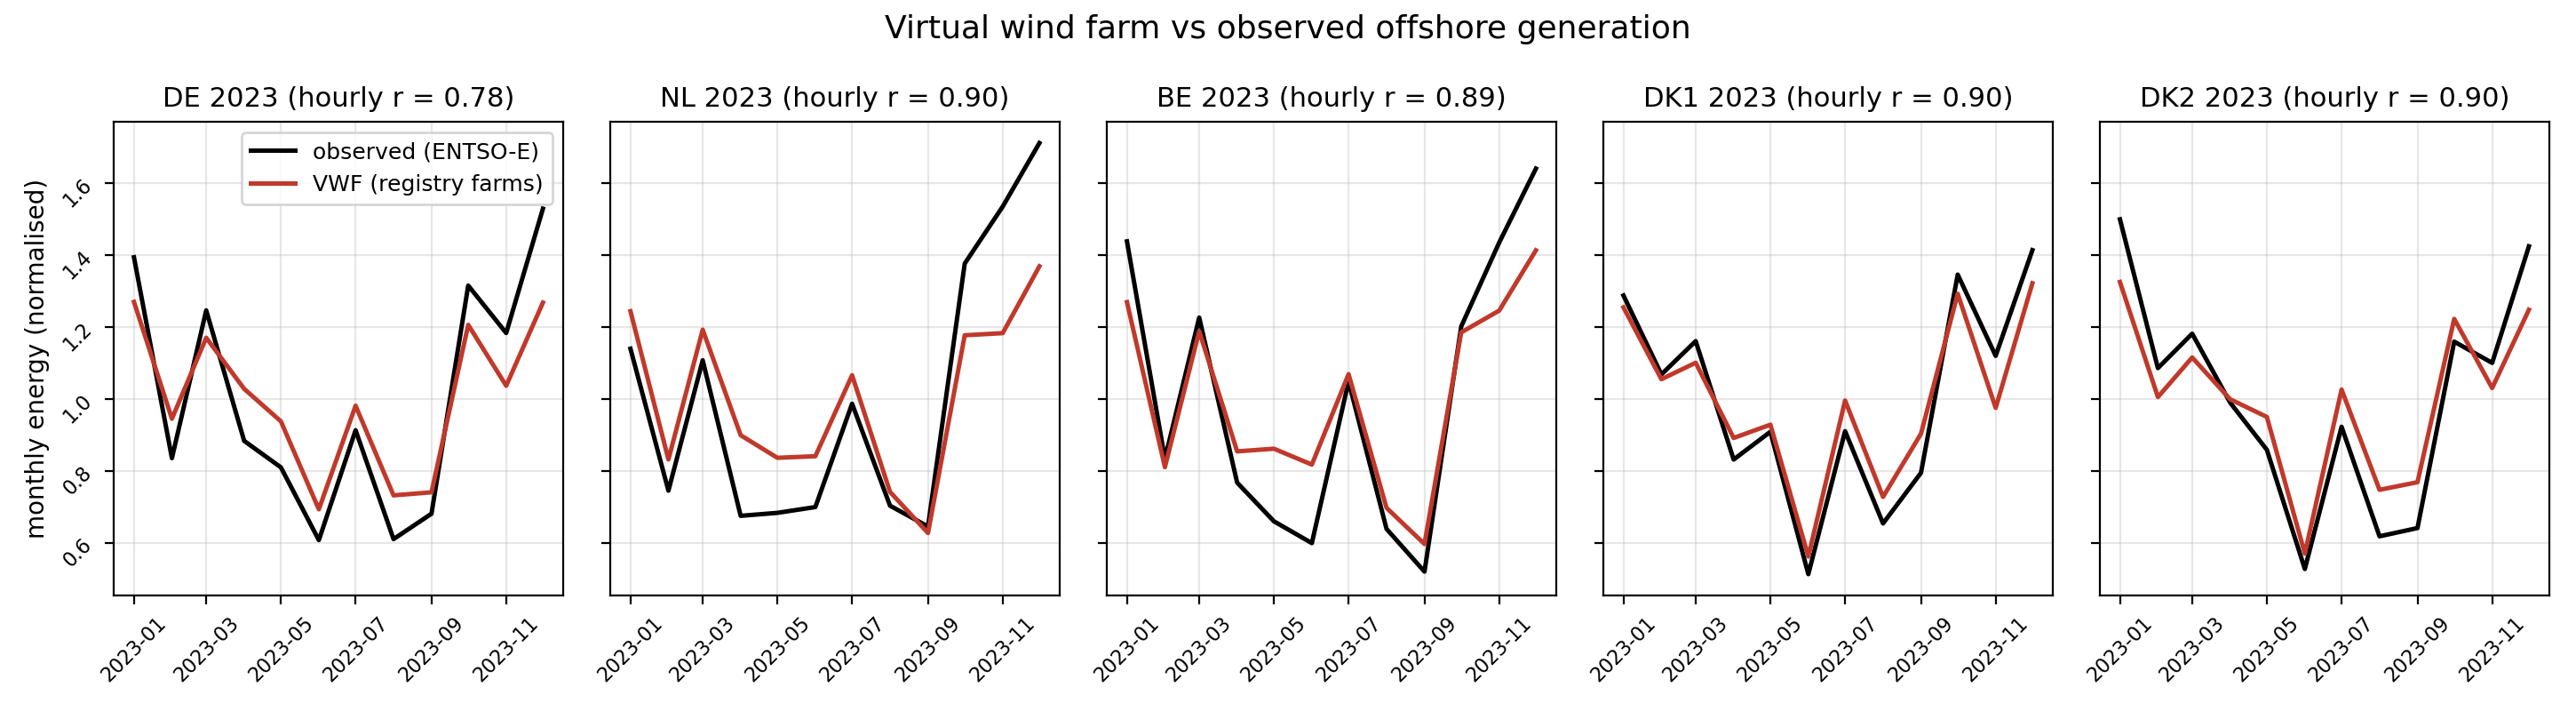
\includegraphics[width=0.95\textwidth]{fig_vwf_vs_observed}
    \caption{The modelled wind farms checked against observed offshore
    generation in 2023. Monthly energy from the modelled farms, normalised
    (red), against the metered fleet in the same zone (black). The median hourly
    correlation is 0.88 and the monthly correlation 0.95.}
    \label{fig:vwf_vs_observed}
\end{figure}

The timing of the output is what matters, because capture value weights
prices by when a farm generates. The modelled output does sit above the metered
figures in absolute terms, since it does not subtract every loss a real farm
incurs. This difference in level does not affect the results, because capture value is
a ratio with generation on both sides, and the farm enters the model's inputs
only through correlations, which are unchanged when output is scaled; a
constant error in the level therefore cancels.


\subsubsection{Feature set at bidding zone resolution}\label{sec:features}

Each farm-month gets seven features, following Jacquet's design
\cite{Jacquet2024} with one upgrade, resolution: each is computed for the farm's
\textit{market area}, the bidding zone where zone-resolved data exist (DK1, DK2,
SE4) and the country elsewhere, so the seven Danish farms see DK1 and DK2
conditions rather than a Danish average. Together they turn the cannibalisation
mechanism of Section~\ref{sec:value_problem} into measurable quantities: how
crowded the farm's selling hours are, how exposed its market is, and how much
surplus the system can absorb.

Features 1 and 2 are the hourly correlations of the farm's output with its
area's total variable renewable generation and with its load,
%
\begin{equation}
    \rho^{\mathrm{VRE}}_{f,m} = \mathrm{corr}\bigl(g_{f,t},\,
    G^{\mathrm{VRE}}_{z,t}\bigr), \qquad
    \rho^{\mathrm{load}}_{f,m} = \mathrm{corr}\bigl(g_{f,t},\,
    L_{z,t}\bigr), \qquad t \in m.
    \label{eq:correlations}
\end{equation}
%
The first measures crowding, a farm producing when every other renewable
produces selling into depressed prices; the second measures alignment with
demand, which lifts value. They enter separately so Chapter 4 can read their
contributions apart; their signed difference forms the pattern penalty in the
analytical equation of Section~\ref{sec:mechanism_tools}. Feature 3 is
penetration, the monthly renewable market share $S_{z,m} =
E^{\mathrm{VRE}}_{z,m} / E^{\mathrm{load}}_{z,m}$, which locates the market on
the cannibalisation curve. Features 4 and 5 are monthly gas and carbon prices,
which set the level of the thermal merit order and so how far prices fall when
wind displaces it. Feature 6 is flexibility, storage capacity over renewable
capacity, the system's ability to move surplus out of windy hours.

Feature 7 is interconnection, and it departs from both predecessors on
Efthymiadou's evidence that realised interconnector \emph{utilisation} rather
than installed capacity dampens price volatility
\cite{Efthymiadou2025, Jacquet2024}:
%
\begin{equation}
    I_{\mathrm{int},z} =
    \frac{\sum_{b}\, \overline{|F_{b}|}}{\sum_{b}\, \max_{t} |F_{b,t}|},
    \label{eq:interconnection}
\end{equation}
%
the mean absolute flow on each external border, divided by that border's
capacity and summed across borders. The economic logic is that an
interconnector relieves cannibalisation only when it carries the
windy-hour surplus out of the zone, so its use and not its rated size is what
lifts capture value. Exact definitions, the dropped neighbour-synchronicity
discount and the index's limitations are recorded in
Appendix~\ref{app:assumptions}.

The two models represent cannibalisation differently: the regression model
encodes it through these features, learned from data, while in the system model
it emerges by construction as added wind shifts the merit order. Collinearity is
clean (largest variance inflation factor 2.16), so the feature contributions in
Chapter 4 read as near-independent mechanisms.
% VIF recomputed on the current 2,706-row panel: max 2.16 (carbon), feature 7 = 1.21.
Figure~\ref{fig:fig_C_feature_evolution} shows how each of the seven has moved
since 2017, averaged within each basin. This is the record the model learns
from, and the starting point from which the projection of
Section~\ref{sec:reg_projection} moves them.

\begin{figure}[!htb]
    \centering
    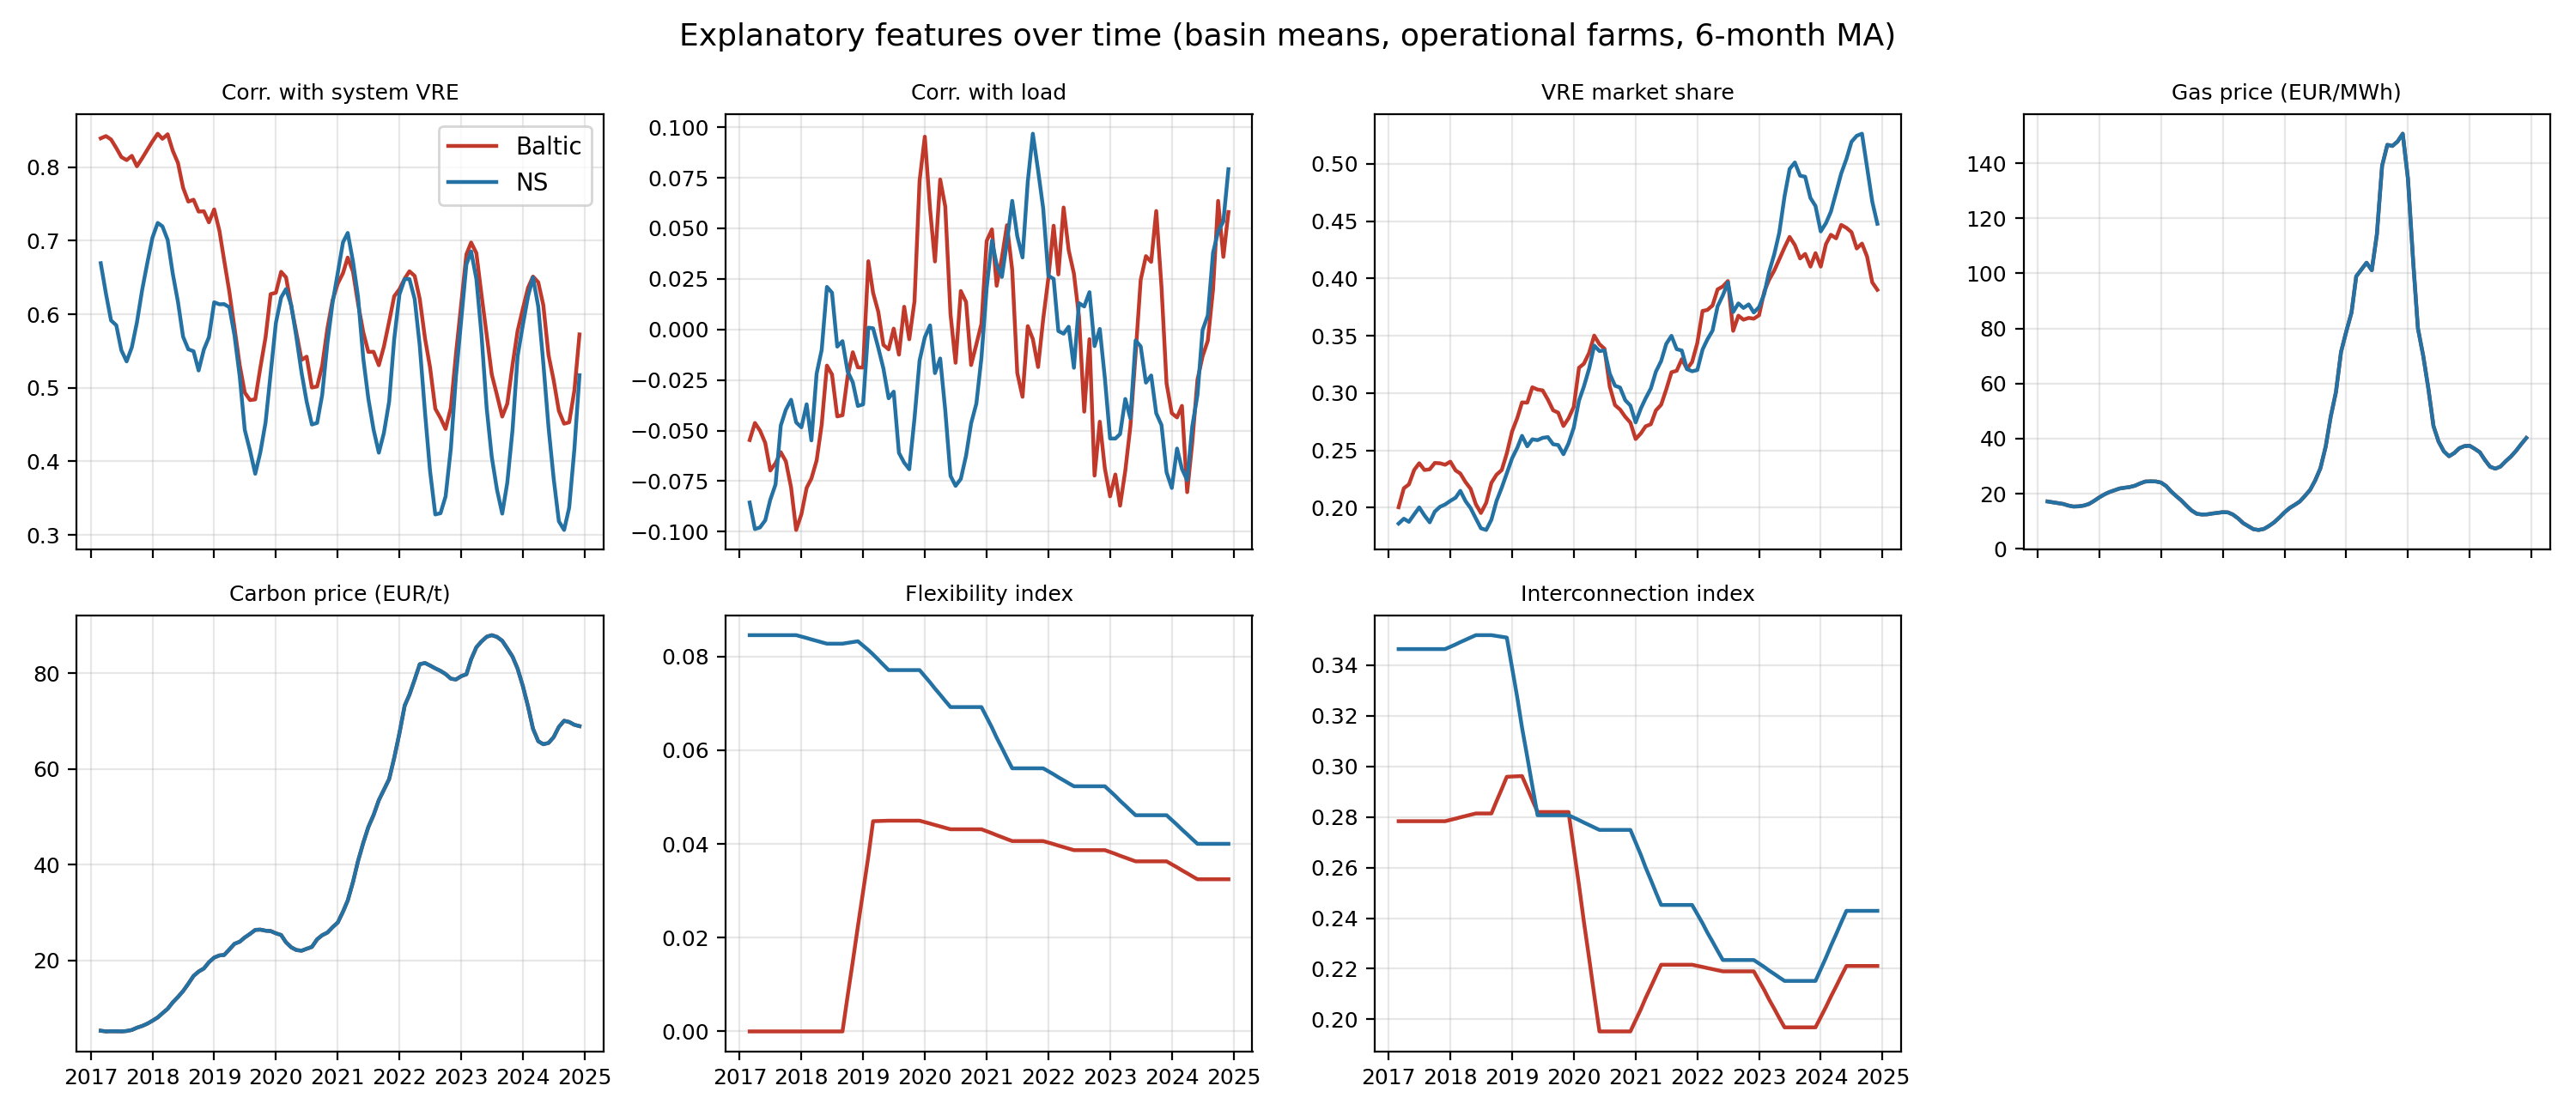
\includegraphics[width=0.98\textwidth]{fig_C_feature_evolution}
    \caption{Basin-mean evolution of the seven features for operational farms,
    2017 to 2024 (six-month moving averages). North Sea in blue, Baltic in red.}
    \label{fig:fig_C_feature_evolution}
\end{figure}

\subsubsection{Algorithm selection and validation}\label{sec:fitting}

In this work five algorithm families are tested: gradient boosting (XGBoost), random forests,
support vector regression, a degree-two polynomial, and ordinary least squares.
Their out-of-fold comparison is tabulated in Chapter~4
(Table~\ref{tab:algorithms}); gradient boosting is the strongest of the five
and carries the analysis.
The training unit is a bidding-zone market observation: a virtual farm at a
representative site in a zone, described by the seven features and labelled with
its monthly capture value. By the principle of Section~\ref{sec:currency} a zone
with observed prices is a valid observation whether or not a farm operates
there, so the panel is all 31 sites over 2017 to 2024, 2,706 zone-months. This
widens the enclosed Baltic from one operational price zone to seven. The
operational farms remain the validation subset. No hyperparameters are tuned, so
the comparison with Jacquet's untuned model is like for like.

How the primary model works also explains what it cannot do. Gradient boosting builds shallow decision trees in sequence, each fit
to the error the ensemble still makes and added at a small learning rate, so
nothing about the functional relationship is assumed in advance, and it
captures nonlinear interactions a single equation would miss, for instance that
interconnection lifts value only once penetration is high enough to need it. The cost of that flexibility is the limit described in
Section~\ref{sec:reg_projection}. A decision tree predicts by averaging the
training observations that fall in each of its leaves, so for an input beyond
the training range it can only return the value of its nearest boundary leaf,
giving a constant response. It interpolates well and does not extrapolate at
all, by construction, which is the reason a second model built from system
structure is needed for the future.

Validation is layered, because one scheme can flatter a panel model, and
all of them rest on one discipline, \textit{out-of-fold prediction}: a
prediction made by a model that never trained on that point. The schemes
differ only in what they withhold.

\begin{itemize}
    \item \textbf{Random five-fold cross-validation} withholds individual
    farm-months. It reproduces Jacquet's scheme, but for panel data it leaks:
    other months of the same farm stay in training, so the model is never asked
    about an unfamiliar farm.
    \item \textbf{Grouped five-fold cross-validation}, the headline scheme,
    withholds entire farms. Each farm-month is predicted by the one model copy
    blind to its farm, and the stitched series, every farm-month predicted once,
    is what all grouped metrics in Chapter 4 score.
    \item \textbf{A chronological split} trains through 2022 and tests on 2023 to
    2024. It withholds the future and stress-tests extrapolation across the
    post-crisis regime change.
    \item \textbf{Leave-one-year-out} fits on every other year and predicts the
    held-out one. Where the single chronological split conflates two failures,
    inability to forecast any year and inability to cross the 2021 to 2022 regime
    break, this separates them year by year, matching the multi-year temporal
    suites of both predecessors.
    \item \textbf{Basin-transfer fits} train on one sea and test on the other, to
    probe whether the learned relationships are basin-specific.
    \item \textbf{A variant excluding 2022} mirrors Jacquet's removal of the
    gas-crisis months.
\end{itemize}

The stitched out-of-fold series is exported for the three-way comparison: when
Section~\ref{sec:triangle} sets the regression against observation in a Danish
zone, the prediction comes from a model that never saw a Danish farm.

\subsubsection{Interpretation of the fitted model}\label{sec:mechanism_tools}

Two tools are used to read an explanation out of the fitted model. The first is
SHAP, short for SHapley Additive exPlanations, which splits each prediction into
a contribution from each of the seven quantities and is computed on the data the
model was fitted to.

SHAP gives the size of each contribution but not the shape of the relationship,
so Jacquet's analytical equation is refitted as the second tool
\cite{Jacquet2024}. Its starting point is that a farm selling in random hours
would have a capture value of one, and cannibalisation is what subtracts from
that one:
%
\begin{equation}
    \mathrm{CV} \;=\; 1
    \;-\; B\,\frac{M_{\mathrm{WF}}}{M_{\mathrm{BZN}}}\,S
    \;-\; C\,M_{\mathrm{WF}}\,
    \bigl(0.202\,p_{\mathrm{CO_2}} + p_{\mathrm{gas}}\bigr)^{\gamma},
    \label{eq:analytical}
\end{equation}
%
where $S$ is the renewable market share and $p_{\mathrm{gas}}$ and
$p_{\mathrm{CO_2}}$ are the monthly gas and carbon prices, folded together by
the emission intensity of gas. The first subtracted term represents cannibalisation through the pattern
penalty of Section~\ref{sec:features},
$M_{\mathrm{WF}} = \mathrm{sign}(\rho_{\mathrm{VRE}} -
\rho_{\mathrm{load}})\,|\rho_{\mathrm{VRE}} - \rho_{\mathrm{load}}|^{\alpha}$,
which grows when a farm's output follows the system's renewables more closely
than it follows demand, is scaled by the market share $S$, and is divided by
the buffering term
$M_{\mathrm{BZN}} = (I_{\mathrm{int}} + I_{\mathrm{flex}})^{\delta}$, in which
interconnection and flexibility absorb the surplus. The second subtracted term
represents the distortion of capture value by fuel prices.

Each constant controls one part of the mechanism: $\alpha$ sets how sharply the
penalty grows as a farm's output becomes more crowded, $B$ sets the overall
strength of the cannibalisation term, and $\delta$ sets how strongly
interconnection and flexibility protect against it. The constants are fitted
separately for each basin by least squares within fixed bounds, with confidence
intervals obtained by resampling whole farms; the fitted values are in
Appendix~\ref{app:assumptions}.

The fitted constants cannot be compared between the basins one at a time,
because different combinations of them produce almost the same curve: a
stronger crowding penalty, through a larger $\alpha$ or $B$, can be offset by
stronger buffering, through a larger $\delta$, and the fit cannot fully
separate the two. What the fit does pin down is the behaviour of the equation
as a whole. The two basins are therefore compared on what their fitted
equations predict, namely how much capture value falls when penetration rises,
calculated for both basins at the same market conditions so that the
comparison reflects the equations and never a difference in circumstances.

\subsubsection{Projection with the regression model: approach and limitations}
\label{sec:reg_projection}

Projecting a farm that has not been built means giving each of the seven
quantities a future value.

\begin{itemize}
    \item The two pattern correlations are held at the site's recent values,
    since they follow from its weather and its position on the grid
    \cite{Jacquet2024}.
    \item Penetration is scaled by the growth in renewable generation relative
    to the growth in demand in the TYNDP scenario.
    \item Gas and carbon prices are taken from the scenario.
    \item Flexibility grows with the battery fleet in the scenario.
    \item Interconnection is held at its recent value. This is mildly optimistic,
    since transfer capacity is unlikely to keep pace with wind, and a
    sensitivity is reported alongside.
\end{itemize}

Twelve sets of inputs are built for each year, one per month, and the predicted
capture values are averaged, so the projection keeps the site's own seasonal
pattern.

The decisive test is whether the model is being asked about conditions it has
seen. A projection is trusted only if all seven quantities lie inside the range
covered by the training data, because outside that range the model has nothing
to learn from.

A check on each quantity separately would be insufficient, however, because a
projection can sit inside the range of every quantity taken one at a time and
still be a combination that never occurred, as the seven do not vary
independently. A stricter test,
following Jacquet, asks whether the projection lies inside the region the
training data occupy in all seven dimensions at once, using its convex
hull. Where a projection fails, the prediction is repeated with the offending
quantity capped at its training maximum, which shows whether the answer depends
on the part of the range the model has never seen.

The equation of Section~\ref{sec:mechanism_tools} is exempt from this limit,
being a formula rather than a set of decision trees, and can therefore be
evaluated at any input, including values outside the
training range. It is projected on the same scenario inputs given to the system
model, which gives a third independent estimate. It differs from Jacquet's use
of it in one way. He holds the pattern correlations fixed, whereas in this work the
Baltic projection lets the correlation with system wind rise towards the level
the built-out Baltic zones already show, and lets interconnection utilisation
fall as wind grows faster than transfer capacity
(Appendix~\ref{app:assumptions}).

\subsection{The system model (PyPSA-Eur)}\label{sec:system}

\subsubsection{Price formation in PyPSA-Eur}\label{sec:pypsa_how}

PyPSA-Eur is the European configuration of PyPSA \cite{Horsch2018}, an open
workflow that assembles a model of the European power system from public data.
The transmission grid comes from ENTSO-E maps, the power plants from open
databases, the weather from the same ERA5 data used for the virtual wind farm,
and demand from historical load. The thousands of connection points in the real
grid are grouped into a smaller number of representative nodes, which is the
setting that trades spatial detail against the size of the problem to be solved.

The model finds the cheapest way to meet demand in every hour of a year, subject
to the capacity of every plant and every line. That problem is a linear program,
so the solution found is the true optimum rather than a good approximation, even
with tens of millions of variables. It is solved with the barrier algorithm in
Gurobi.

Two of its outputs are used in this thesis. The first is how much every generator produces
in every hour. The second is the shadow price at every node, which is what it
would cost to serve one more unit of demand there in that hour. In a windy hour
the last unit needed comes from wind, which costs almost nothing to run, so the
price falls towards zero. In a still hour it comes from a gas plant, which sets
a much higher price. A real market clearing on marginal cost prices in the same
way, which is why the shadow price is used as the wholesale price.
Practical details are in Appendix~\ref{app:assumptions}.

\subsubsection{Scope and configuration}\label{sec:pypsa_config}

The model covers the fourteen countries around the two basins. They are
clustered into thirty nodes, with more nodes given to the markets that carry
most of the offshore wind, and solved at full hourly resolution. Thirty nodes is
finer than one node per country, so Denmark separates into its two  bidding
zones, and congestion within a zone as well as between zones is priced at each
node.\footnote{In a zone represented by more than one node, the denominator of
capture value is the price averaged across that zone's nodes, which corresponds
to the single zonal price of Equation~\ref{eq:value_factor}, while the numerator
weights each generator by the price at its own node. The two are identical
wherever offshore wind is present at all of a zone's nodes, which is the case in
the single-node Baltic zones that carry the headline result. A difference arises
only in zones that also contain inland nodes with no offshore wind.}

Transmission is held at today's capacity throughout. Congestion is
priced as it exists now, which
makes the projection conservative. Section~\ref{sec:robustness} solves the
opposite case, with transmission free to expand.

Generation fleets are set to the capacity installed in each modelled
year, and topped up where the database falls short of national statistics. For
2023 and 2024, fuel and carbon prices are set to the observed annual
averages.

\subsubsection{Historical baselines and calibration}
\label{sec:calibration_method}

Three past years are solved. 2023 is the main validation year. 2019 is added so
that the model is tested both before and after the energy crisis, in a cheap-gas
world and an expensive one. 2024 is added because it provides validation points
at the highest penetrations yet observed, which is what the bias correction of
Section~\ref{sec:bias_method} is fitted on.

The calibration is judged on price levels and on capture value. Price levels
are compared zone by zone against observed
day-ahead prices, using a normalised absolute error, because percentage errors
are undefined when prices are negative. Capture value, the quantity the thesis
uses, is checked separately, and a third value is calculated alongside it to
locate any error: the model's own generation valued at observed prices. If that
hybrid value matches observation while the fully modelled value does not, the
modelled prices carry the error and the modelled generation is sound.

Solver settings are the same for the past years and for the projections, so the
bias correction is applied to prices formed in exactly the same way as the ones
it was fitted on. The settings are listed in Appendix~\ref{app:assumptions}.

\subsubsection{Projection to 2030 and 2040}\label{sec:projection}

The projection solves six scenarios from the 2024 TYNDP trajectories on the
validated 2023 network. Four follow National Trends, the pathway that tracks
existing national policies: for each of 2030 and 2040, one solve installs the
Baltic offshore capacity the plan schedules, and one an accelerated variant in
which the Baltic builds further. The remaining two repeat the accelerated 2040
case under the plan's other demand pathways, Distributed Energy and Global
Ambition, which electrify more of Europe's energy demand. All six are listed
with their results in Table~\ref{tab:projection}.

Two assumptions govern demand. The base year is 2019, the last year before the
crisis depressed consumption, and demand in each scenario year is that base
scaled by the country's TYNDP growth factor, with documented substitutes for
the two countries the scenario tables omit. Capacity targets are adopted in
full: where a scenario prescribes more capacity than the clustered nodes can
physically host, the whole target is still installed and the excess is
recorded, so no capacity is dropped without record.

Six further corrections close the remaining gaps between renewable-only
scenario tables and an electricity-only model, and Table~\ref{tab:corrections}
states each with its implementation and rationale. All act in the same
direction, preventing the model from generating surplus zero-cost electricity
that would make capture value look higher than it should be.
\begin{table}[H]
\centering
\small
\caption{The six corrections, labelled A to F, applied to the scenario inputs
before the 2030 and 2040 solves. The TYNDP scenario tables prescribe renewable
capacity only and the system model represents the electricity sector only, so
each correction closes a gap that combination leaves open. Each row states
what is changed and why.}
\label{tab:corrections}
\begin{tabular}{l >{\raggedright\arraybackslash}p{10.8cm}}
\toprule
\textbf{Correction} & \textbf{What is changed, and why} \\
\midrule
A. Coal phase-out & German and Polish coal and lignite capacity is reduced
year by year in line with the legislated closure schedules, which the scenario
tables leave out. \\
\addlinespace
A2. Polish nuclear & Poland's announced 3.9~GW nuclear programme is added from
2040, since the scenario tables add no thermal capacity at all. \\
\addlinespace
B. Offshore caps & Danish, Finnish and Swedish offshore capacity is capped at
the nationally planned levels, removing capacity that the scenario tables
wrongly assign to these zones through planned energy islands. \\
\addlinespace
C. DK1/DK2 split & The Danish offshore total is split 60/40 between the DK1
and DK2 bidding zones by 2040, because the default allocation by wind resource
alone gives DK2 too little. \\
\addlinespace
D. Hydrogen demand & Electrolysers with a fixed hydrogen demand are added in
each country, alongside a priced import alternative that sets the level at
which producing hydrogen is worthwhile. This gives surplus electricity a use;
without one, an electricity-only model produces implausibly many hours priced
at zero. \\
\addlinespace
E. Demand base year & Demand is projected from a 2019 base using the TYNDP
growth factors, with documented substitutes where factors are missing, because
the factors are quoted relative to 2019 and two countries are absent from the
scenario tables. \\
\addlinespace
F. Shortage pricing & Demand response is added at 5\,\% of peak load, offered
at 400~\euro/MWh, with involuntary curtailment at the 4{,}000~\euro/MWh price
cap, so that hours of shortage are priced the way a real auction prices them. \\
\bottomrule
\end{tabular}
\end{table}
\subsection{Validation against observed prices}\label{sec:confrontation}

\subsubsection{Comparison with observed ENTSO-E prices}\label{sec:triangle}

For every zone and year in which offshore generation was observed,
which is five zones across 2019, 2023 and 2024, the same capture value is
estimated three times: from observation, by the system model, and by the
regression model. The regression estimate comes from a copy that never saw that
zone's farms.

These three estimates are mutually independent, since the regression estimate
uses nothing from the farm it is predicting, the system estimate uses no
market prices at all, and the observed value comes from outside both models.
Agreement between them is therefore informative, and where they disagree, the pattern of the
disagreement shows which model is at fault. This is a different exercise from
the hybrid value of Section~\ref{sec:calibration_method}, which
mixes modelled generation with observed prices in order to locate an error
inside the system model.

\subsubsection{Bias correction procedure}\label{sec:bias_method}

The comparison above shows the system model reading high in small congested
zones, and by more where more offshore wind has been built (Chapter 4). That
relationship is what the correction uses. A straight line is fitted by least
squares through the measured overstatements against the zone's offshore
penetration, meaning its offshore generation as a share of consumption, and the
fitted line is subtracted from the model's output:
%
\begin{equation}
    \mathrm{CV}_{\mathrm{corr}} = \mathrm{CV}_{\mathrm{raw}}
    - \bigl(\hat{a} + \hat{b}\,\pi\bigr),
    \label{eq:bias}
\end{equation}
%
where $\pi$ is the zone's modelled offshore penetration and $\hat{a}$ and
$\hat{b}$ are the fitted intercept and slope. The model's own penetration is
used, not the observed one, because the correction is applied to the model's
own output. This quantity is narrower than the all-renewables share used as a
feature by the regression model.

\subsubsection{Decomposition and scoring of the difference between the models}
\label{sec:gap_method}

Section~\ref{sec:triangle} establishes that the two models differ and four further
tests establish why: where they agree, where they part, how each compared
to the observed counterparts, and how their projections compare.

\textbf{Channel decomposition.} Both models compute capture value with the same
formula (Equation~\ref{eq:value_factor}) from different inputs. The regression
model uses the virtual farm's generation valued at observed day-ahead prices,
and the system model uses its own generation valued at its own prices.
Substituting one input at a time, and averaging over both possible orders,
divides the difference between their answers exactly into a generation part and
a price part, with nothing left over and no dependence on which substitution is
made first. The price part divides again by re-pricing against observed prices
with negative values set to zero, which isolates the effect of the linear
program being unable to produce them. A fourth part carries the way the network
is represented, and a small remainder absorbs the out-of-fold fit and the
averaging of prices across nodes.

\textbf{Scoring both models on targets neither has seen.} Comparing the two
directly would favour the regression model, since it is fitted to the record it
would be scored on. It is therefore refitted with the target withheld, using the
grouped schemes of Section~\ref{sec:fitting}, once leaving out each bidding zone
and once leaving out each year. Whole blocks are withheld rather than individual
observations, because capture value is correlated in space and in time, and
withholding single points would leave near-duplicates in the training set
\cite{Roberts2017}. Both models are then scored on the same zone-months against three measures.

Mean absolute error and root mean squared error are
reported on the natural scale of capture value, which is dimensionless and
bounded, so the usual objections to percentage errors do not apply
\cite{HyndmanKoehler2006}. Signed bias records the direction of each model's
error. A skill score compares both against the benchmark of assuming that a farm
simply earns the average price. Because zone-months within a zone are not
independent, the difference between the two models is tested by a paired
comparison with a bootstrap that resamples whole zones \cite{DieboldMariano1995}.

Accuracy alone would not settle the question, since two models can be equally
accurate and have different errors. Each model's error is also separated,
following Theil \cite{Theil1966}, into three parts: a consistent offset, a
failure to match how much the observations vary, and mistiming, which is the
error that remains once level and spread are both right. The arithmetic is in
Appendix~\ref{app:forecast_checks}.

\textbf{Backtesting the projection.} The test above scores the models but not
the act of projecting, which also requires future inputs to be built. The
regression model is therefore refitted on data up to 2021 and asked for 2023 and
2024 twice: once from the inputs that occurred, and once from inputs
constructed the way a projection must construct them, with weather terms set to
each farm's pre-2022 average and system terms carrying the pre-2022 monthly
shape. The system model is fitted to nothing, so it is already a projection, and
it is scored on the same targets. The difference between the two regression runs
is the cost of building the inputs, and the difference between either of them
and the system model is the like-for-like comparison. The constructed inputs use
the annual levels that occurred, and not those a forecaster in 2021 would have
assumed, so the test grants perfect foresight of the scenario.

\textbf{Comparing the two projections.} Both models are run on the same TYNDP
scenarios, so the only difference between their answers is the model. They are
compared at 2030, where both are still inside the observed range, and at 2040,
where the regression model is not. Because 2040 cannot be checked against
observation, both projections are also placed beside published estimates of
capture value at high penetration, recording the renewable share at which each
published figure was measured. Recording that share matters, because a benchmark measured at a share on which
the regression model was trained cannot separate the two models, since a model
reproducing conditions inside its training range will match it regardless of
its behaviour beyond that range, and only a benchmark from an already
saturated market is decisive.

\textbf{The exclusion of DK2.} DK2 is left out of the scored set, on a criterion
fixed before the results were seen. Its prices are set partly by plants that
must keep running and by combined heat and power, neither of which a linear
program represents, and this shows in its 264 observed hours of negative prices
in 2023 against the system model's zero. It remains in the regression model's
training data, and every headline figure is also reported with DK2 included.

\subsubsection{Robustness, model runs and reproducibility}\label{sec:robustness}

The projected values rest on assumptions about fuel prices, the transmission
grid, the pricing of shortage, and the six scenarios chosen, and the
sensitivity of the results to each of these is tested in turn.

\begin{itemize}
    \item \textbf{Gas prices.} The assumed gas price is varied by re-solving
    three buildouts across five gas prices, which separates the effect of the
    buildout from the effect of fuel costs.
    \item \textbf{Transmission.} The grid assumption is inverted by re-solving
    all six scenarios with transmission free to expand, which gives the bound
    opposite to the grid held at today's capacity
    (Section~\ref{sec:pypsa_config}).
    \item \textbf{Shortage pricing.} The treatment of shortage is tested by
    recalculating every capture value with the shortage-priced hours removed,
    meaning those in which supply is tight and the price rises to the levels
    set by demand response or the price cap, which establishes that the result
    does not rest on a few extreme prices.
    \item \textbf{Scenario choice.} The dependence on the six chosen scenarios
    is tested with a fast approximation of the system model, trained on 76
    solved networks, which prices a scenario in milliseconds and so allows far
    more scenarios to be examined than could be solved directly.
\end{itemize}

The results of all four sensitivity analyses, together with the validation of
the fast approximation, are collected in Appendix~\ref{app:robustness}.

Every model run behind Chapter 4 is listed in Table~\ref{tab:runs} of
Appendix~\ref{app:repro}, so each number can be traced to the run that produced
it, and the whole procedure is scripted from the raw downloads to the final
tables. A single command re-solves everything in about three hours, every
reported number can be regenerated from public data, and the solver settings
and assumptions are fixed in Appendix~\ref{app:assumptions}.



\subsection{Value-adjusted cost of energy}
\label{sec:vlcoe_method}

Capture value on its own does not tell an investor whether to build, so this
section turns it into a cost. The measure used is the value-adjusted levelised
cost introduced in Section~\ref{sec:vlcoe_lit}: the levelised cost divided by
capture value, which gives the average wholesale price a site must earn to break
even. It is used because capture value enters it directly, so a projected
fall in value becomes a rise in the price a site needs.

\subsubsection{Mapping levelised cost}\label{sec:cost_field}

Costs are mapped at the resolution of the wind resource rather than that of the
system model. Three geospatial datasets are used: capacity factor from the
Global Wind Atlas at roughly two kilometres \cite{GlobalWindAtlas}, water depth
from GEBCO \cite{GEBCO2014}, and distance to shore, calculated on the same grid.

Capital cost rises with both depth and distance, since deeper water requires heavier
foundations, with a step change beyond 60 metres where fixed-bottom foundations
give way to floating ones, and sites further from shore require longer export
cables. Capital cost is modelled in segments, one for each of these
regimes, anchored to the PyPSA-Eur cost database and IRENA's 2024 review
\cite{Horsch2018, IRENA2025Costs} and set out in
Appendix~\ref{app:assumptions}. It is annualised at a 7\,\% cost of capital over
a life of 27 to 30 years.

The levelised cost is the annualised cost divided by the energy a megawatt of
capacity delivers in a year,
%
\begin{equation}
  \mathrm{LCOE}(d,\ell,y) \;=\;
  \frac{\mathrm{CRF}\,\lambda(y)\,\mathrm{CAPEX}(d,\ell) + f_{\mathrm{OM}}(\ell)}
       {\mathrm{CF}\cdot 8760},
  \label{eq:lcoe}
\end{equation}
%
and it is computed for every cell at all three years. The full set of maps is in
Appendix~\ref{app:atlas}.

\subsubsection{Combining cost with capture value}\label{sec:vlcoe_def}

The value-adjusted cost (Equation~\ref{eq:vlcoe}) is calculated for each cell by
dividing its levelised cost by the capture value of the zone it sits in, taken
from the solved networks.

The same inputs give a second quantity, the net value of a site, which is the
revenue it captures less its annualised cost,
%
\begin{equation}
  \mathrm{NV}(d,\ell,y) \;=\;
  \underbrace{\mathrm{CF}\cdot 8760\cdot \mathrm{CV}\cdot \bar p}_{\text{captured revenue}}
  \;-\; \big(\mathrm{CRF}\,\lambda(y)\,\mathrm{CAPEX} + f_{\mathrm{OM}}\big).
  \label{eq:netvalue}
\end{equation}
%
The value-adjusted cost says what price a site needs. The net value says how
much money it makes or loses at a given price. Both are reported for a merchant
project, meaning one that sells at market prices with no support contract.

\subsubsection{Pricing interconnection and robustness checks}\label{sec:vlcoe_grid_method}

Capture value enters the denominator of the value-adjusted cost, so any change
in capture value changes the average wholesale price at which a site's
revenues cover its costs. The effect of transmission on that break-even price
is isolated by computing Equation~\ref{eq:vlcoe} for 2040 twice, once with the
per-zone capture values of the grid held at today's capacity and once with
those of the grid free to expand, while the levelised cost is held identical
in both. Transmission is a separate investment that leaves the cost of
building and operating a farm unchanged, so only the revenue side of the
calculation moves, through capture value, and the difference between the two
computations is reported for each basin as the reduction in the break-even
price, in \euro/MWh.

Whether the value-adjusted cost rises or falls to 2040 is then tested across 27
combinations of three cost assumptions: the weighted average cost of capital at
5, 7 and 9\,\%, a multiplier on capital cost of 0.8, 1.0 and 1.2, and a 2040
learning rate of 5, 12 and 25\,\%. The absolute cost level cancels when the 2040
value-adjusted cost is divided by the 2025 one, so the direction depends only on
whether cost falls faster than capture value. That same ratio also gives
directly the rate of cost decline that would be needed to hold the
value-adjusted cost flat.

\subsection{Methodological justification}\label{sec:method_why}

Each choice above follows from one of the research questions.

\begin{itemize}
          \item \textbf{Two models rather than one}, to compare them and decide
    which is better suited to representing the present and forecasting the
    short term, and which to forecasting the long term.
    \item \textbf{Gradient boosting for the regression model}, because it scores
    best of the five algorithms tested (Table~\ref{tab:algorithms}), and because
    the way it fails is visible: beyond its training range it returns a
    constant, which can be detected and reported.
    \item \textbf{PyPSA-Eur for the system model}, because it is the only option
    combining open code and open data, the full European network, resolution at
    the level of bidding zones, and hourly dispatch.
    \item \textbf{Every scenario solved twice}, with the grid at today's
    capacity and with it free to expand, because the difference between the two
    isolates the part of the erosion caused by congestion, which is what the
    second research question asks.
    \item \textbf{The value-adjusted cost}, because it carries the measured
    capture value into the decision an investor makes.
\end{itemize}

The limits of each of these choices are recorded in
Appendix~\ref{app:assumptions}.
% ============================================================================
% Chapter 4 · Results
% Style: no em dashes. Plain declaratives, one idea per sentence. Lead with the
% finding; push caveats to a trailing clause or the appendix. Each section ties
% to its research question. Validate-then-project rhythm; DK2 recurs.
% ============================================================================

\section{Results}\label{sec:results}

This chapter reports the results in the order of the research questions.
Section~\ref{sec:measured} establishes the measured record.
Sections~\ref{sec:trust} and~\ref{sec:why_differ} validate the two models
against observation, examine why they differ, and settle which is used for
what, and Section~\ref{sec:projection_results} then projects the committed
buildout to 2030 and 2040. Section~\ref{sec:mechanism} explains what drives
the erosion and how much of it system design removes, and
Section~\ref{sec:vlcoe_results} carries the results into the decisions they
inform, the break-even price a site must earn and where to build. 




% ----------------------------------------------------------------------------
\subsection{The empirical record of capture value}\label{sec:measured}

This section establishes where the two basins stand today, on eight years of
observed prices.

\subsubsection{Measured capture value, 2017 to 2024}
\label{sec:eight_years}

Revenue per megawatt of installed capacity has three parts that change over
time: how much a farm generates, the average price in its market, and capture
value. Figure~\ref{fig:revenue_decomp} separates them for 2017 to 2024.
Generation is flat across the period, and the average price rises and falls
with the gas crisis, moving in the same direction in every market. Only capture value
declines steadily, and it is the term this chapter measures.

\begin{figure}[!htb]
    \centering
    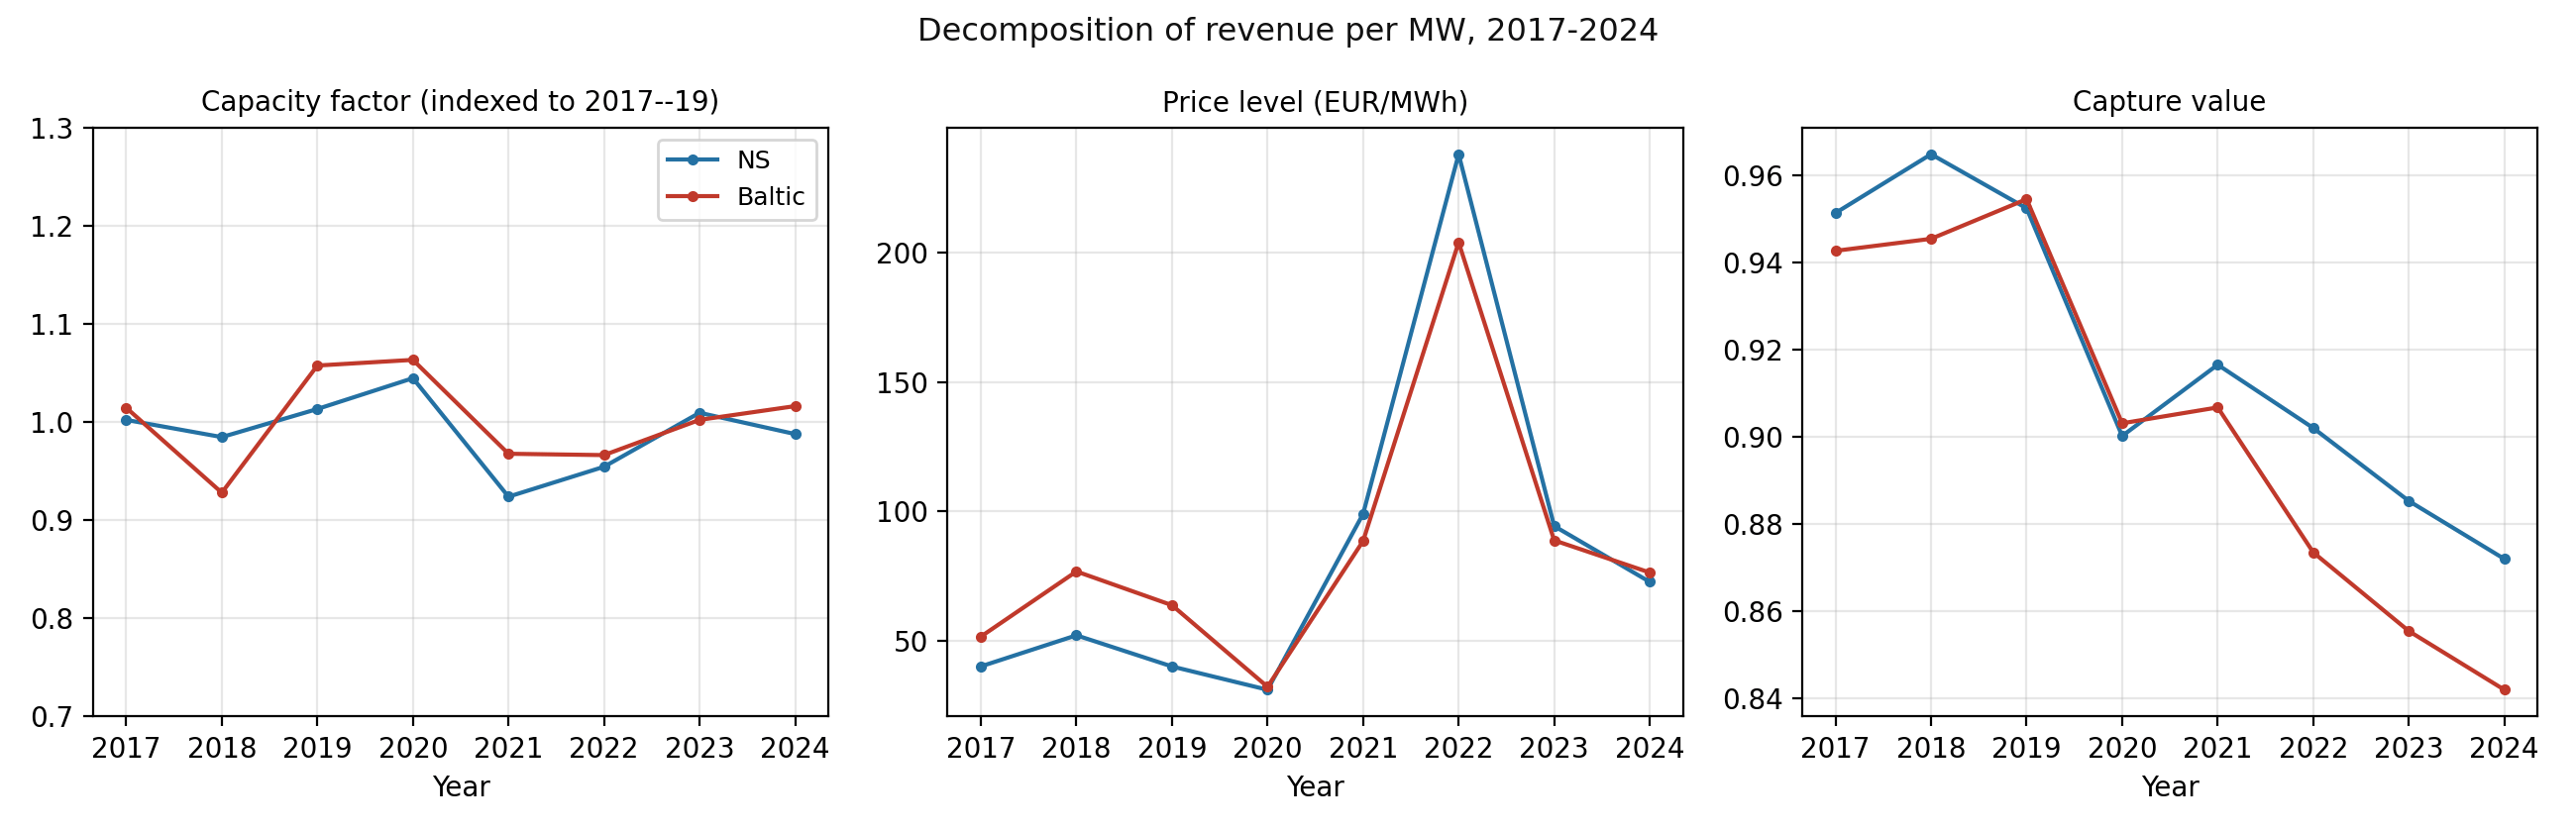
\includegraphics[width=0.98\textwidth]{fig_revenue_decomp}
    \caption{The three parts of revenue per megawatt, 2017 to 2024. Generation
    (left) is flat and the average price (centre) follows the gas crisis, while
    capture value (right) declines steadily.}
    \label{fig:revenue_decomp}
\end{figure}

Figure~\ref{fig:group_arc_observed} shows capture value for the four groups of
farms defined in Section~\ref{sec:farm_data}. Over 2023 and 2024 the Baltic
zones that have built little offshore wind capture 0.883 of the average price
and the North Sea 0.879, which puts the two level. The lower Baltic average comes from the other two
groups: DK2 and SE4, which have already built out, at 0.766, and Finland at
0.568, where nuclear generation holds prices down.

\begin{figure}[!htb]
    \centering
    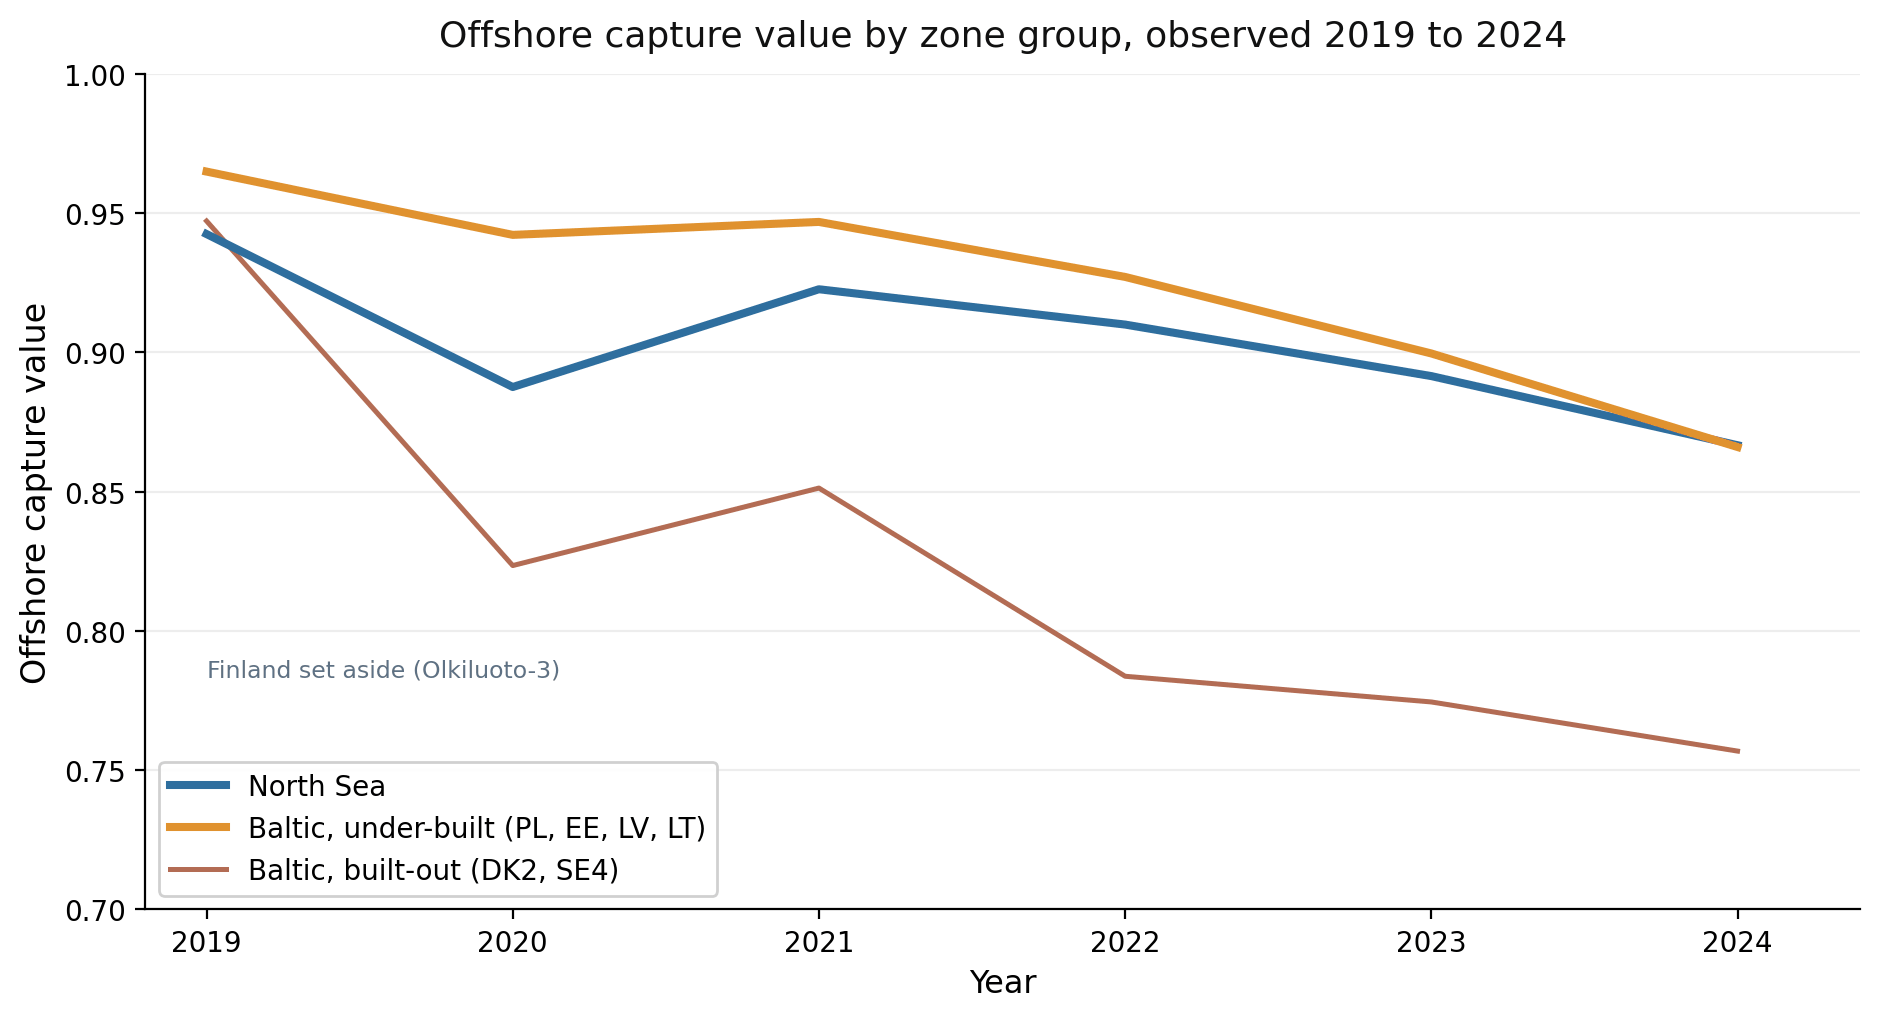
\includegraphics[width=0.9\textwidth]{fig_group_arc_observed}
    \caption{Observed capture value by group of zones, 2019 to 2024. The Baltic
    zones with little offshore wind capture the same share as the North Sea,
    while DK2 and SE4, which have built out, capture less than both.}
    \label{fig:group_arc_observed}
\end{figure}

Table~\ref{tab:archetype_measured} adds the measured values to the expectations
set out in Chapter 2, and most of those expectations are incorrect. Germany was
expected to be the most eroded market, yet its offshore farms capture 0.904. Its
offshore fleet generates at different times from its much larger onshore fleet,
and it is the onshore fleet that pulls the national figure down to 0.76
\cite{Stiewe2025}. Denmark's national 0.822 combines two very different price
zones, which are separated below.

The Baltic was expected to capture close to 1.0, above the North Sea, because
little capacity has been installed there. The measured values are level with the
North Sea. Poland captures 0.922, slightly above it. Estonia, Latvia and
Lithuania capture 0.86 to 0.88, slightly below. The group averages 0.88 against the North
Sea's 0.879, with almost none of the planned capacity built. Sweden at 0.729 and
Finland at 0.568 sit lower, but each rests on a single farm in a market
dominated by nuclear and hydro generation, where a surplus of constant output
holds prices down as much as wind does. They are read as signals about their
price zone more than about the farm, and the comparison holds without them. The
hydro premium predicted by Hirth \cite{Hirth2013} does not appear in the Baltic
after 2022.

\begin{table}[!htb]
\centering
\small
\setlength{\tabcolsep}{4pt}
\caption{Expectations from Chapter 2 compared with measurement. Measured values
are farm-level capture values for 2023 and 2024, calculated from modelled farm
output and observed zonal prices. The Swedish and Finnish rows rest on one farm
each and describe their price zone more than a typical farm, which is discussed
in Chapter 5.}
\label{tab:archetype_measured}
\begin{tabular}{l c
                >{\raggedright\arraybackslash}p{3.1cm}
                >{\centering\arraybackslash}p{1.9cm}
                >{\centering\arraybackslash}p{1.4cm}
                >{\raggedright\arraybackslash}p{3.3cm}}
\toprule
\textbf{Market} & \textbf{Basin} & \textbf{Expected in Chapter 2} &
\textbf{Measured capture value} & \textbf{Farm months} & \textbf{Outcome} \\
\midrule
Germany & NS & Eroded, declining & 0.904 & 144 & Milder than expected \\
\addlinespace
Netherlands & NS & Eroded & 0.890 & 96 & As expected \\
\addlinespace
Denmark & NS/BS & Eroded, with some buffering & 0.822 & 168 &
Averages two different zones \\
\addlinespace
Sweden & BS & Favourable (hydro) & 0.729 & 24 & Lower than expected \\
\addlinespace
Finland & BS & Favourable & 0.568 & 24 & Lower than expected, one farm \\
\addlinespace
Poland & BS & Very favourable & 0.922 & 48 & Close to expectation \\
\addlinespace
Baltic states & BS & Close to 1.0 & 0.86--0.88 & 72 &
Level with the North Sea \\
\bottomrule
\end{tabular}
\end{table}

Ordering the same zones by how much offshore wind they have built turns the
comparison into a sequence. DK2 and SE4, the most built out, capture least. The
zones with little capacity earn what the North Sea earns. The two basins are
following the same relationship between buildout and capture value,
and the Baltic entered it at the same level, with DK2 and SE4 showing the stage
it has already reached.

Two comparisons show that what sets the value is the price zone a farm sells
into. Four German farms stand in Baltic water but sell into the German market,
and they capture 0.91, the same as German farms in the North Sea. The weather is
Baltic, the market is open, and there is no discount. Denmark gives the reverse
case: DK2 captures 0.784 and DK1 0.854, in the same country and under the
same support scheme, separated only by the price zone their output must be sold
in.

That mix is what makes the Baltic average of 0.84 match no individual zone. It combines
German-priced Baltic farms at 0.91, the enclosed DK2 and SE4 at 0.78, and
Finland at 0.57. The zones with little capacity, level today, are where the
buildout starts, and the enclosed zones at 0.78 show where it leads. For those
enclosed zones, the larger part of the gap to the North Sea comes from limited
capacity to export surplus, and a smaller part from the amount of wind in the
zone itself. After the crisis the local-wind part of the gap shrank while the
interconnection and wind-pattern parts grew\label{sec:gap_opened}. These are the
same two causes measured in Section~\ref{sec:mechanism}.

% ----------------------------------------------------------------------------
\subsection{Validation of the two models}\label{sec:trust}

The supporting tables for the comparisons in this section are in
Appendices~\ref{app:reg_tables} and~\ref{app:triangle}.

\subsubsection{Performance of the regression model}\label{sec:trust_empirical}

The regression model was tested on price zones that were excluded from the
inputs used to fit it. On those zones it accounts for 69\,\% of the variation
in capture value across farms and months. Its estimates are within 0.04 of the observed value in
five of the seven enclosed Baltic zones and within 0.07 in Sweden. The one clear
miss is Finland, at 0.10, where nuclear generation holds prices down in a way
the seven market conditions used as inputs do not describe.

Measuring those conditions separately for each bidding zone, instead of once per
country, raises the score by nine points. Prices are set within zones, and
treating DK1 and DK2 as a single Danish market would hide the difference between
them, which is central to this thesis.

The model's limit emerges once it is fitted on data up to 2022 and asked to
estimate 2023 and 2024, where it performs worse than simply assuming that every farm
has the average capture value. The energy crisis pushed gas and carbon prices
beyond anything in its training data. Leaving out one year at a time confirms
this: the model works well inside the range of conditions covered by its
training inputs, and fails across the break between 2021 and 2022.

\subsubsection{Performance of the system model}\label{sec:trust_system}

The system model is solved with the transmission grid held at its present
capacity, so congestion is priced as it exists today. This makes the absolute
price level less accurate, which matters little in this case. Capture value is a ratio
between the price a farm earns and the average price in its market, so an error
shared by both largely cancels.

Where the grid is strong the ratio matches observation closely. In Germany the
model gives 0.908 against an observed 0.909, and the Netherlands is similar.
Where the grid is congested the model reads too high, and the gap widens as
congestion increases: 0.03 too high in Belgium and 0.06 in DK1. These are
differences in capture value itself, so 0.06 means the model credits Danish
offshore farms with six per cent more of the average price than they earned.
Great Britain and Norway do not pass this check at the resolution used and
are excluded from every aggregate.

Because the model's error runs in one direction only, always crediting farms
with more of the average price than they received, it is a bias in the
statistical sense, and a bias can be traced to its source. The model produces
two outputs that could carry it, the generation of each farm and the price in
each hour, and the two are separated by valuing the model's own generation at
the prices that were actually observed. Most of the error disappears under
that substitution, which shows that the modelled generation is close to
correct and that the bias sits in the modelled prices. The same bias appears
again in 2019 and in 2024, so it is stable from year to year, and an error
that is stable and always in one direction can be measured and subtracted,
which is what the correction of Section~\ref{sec:bias_method} does.

The one zone that cannot be corrected is DK2, where the model reads 0.14 too
high. That zone
had 264 hours of negative prices in 2023, which occur because some plants keep
running even when prices are below zero: combined heat and power stations that
must supply heat, and generators whose subsidy makes it worth paying to stay
online. The system model is a linear optimisation and does not represent
decisions of that kind, so it produces no negative prices at all. This
limitation belongs to the class of model, so DK2 is set aside
(Appendix~\ref{app:robustness}).

\subsubsection{Allocation of models to analytical tasks}\label{sec:division}

When the two models are compared with the same observed record, the regression
model proves the more accurate of the two: across fifteen combinations of
price zone and year, its estimates deviate from the observed capture value by
0.011 on average, against 0.054 for the system model. A difference in this
direction is expected from the way each model is estimated. The regression
model is fitted to the observed prices themselves, so it reproduces market
behaviour that a cost-based simulation cannot, including the hours in which
the price falls below zero. The system model instead derives its prices from
generation costs, and observed prices depart from cost-based prices whenever
something the model does not represent intervenes, such as a plant that must
keep running or a sudden movement in fuel prices. For measuring the present
and the recent past, the regression model is therefore the more reliable
instrument, and the question that remains is whether the same holds beyond the
observed record.

Each model
is used where the evidence supports it. The regression model measures
the present, explains why one farm earns less than another, and supports
short-term projection. The system model carries the projection to 2030 and 2040,
because it derives its prices from costs, and because it
alone can be solved again under a different grid, gas price or level of
flexibility (Table~\ref{tab:model_verdict}).

\begin{table}[!htb]
\centering\small
\setlength{\tabcolsep}{4pt}
\caption{Comparison of the two models across the six tasks the thesis requires
of them. Errors are average deviations from observed capture value over the
fifteen zone-year validation points of Appendix~\ref{app:triangle}; scenario
ranges are measured across the four Baltic 2040 scenarios.}
\label{tab:model_verdict}
\begin{tabular}{>{\raggedright\arraybackslash}p{2.2cm}
                >{\raggedright\arraybackslash}p{3.2cm}
                >{\raggedright\arraybackslash}p{6.9cm}
                >{\raggedright\arraybackslash}p{1.9cm}}
\toprule
\textbf{Question} & \textbf{Task} & \textbf{Result} & \textbf{Conclusion} \\
\midrule
Accuracy on the observed record &
Reproduce the capture value observed between 2017 and 2024 &
The regression model deviates from observation by 0.011 on average and the
system model by 0.054, with the system model's error growing with congestion &
Regression model \\
\addlinespace
The most cannibalised zone &
Reproduce DK2 in 2023, where 0.784 was observed &
The regression model gives 0.798, an error of 0.014, while the system model
gives 0.932, an error of 0.148 &
Regression model \\
\addlinespace
Negative prices &
Reproduce hours in which the price falls below zero &
The regression model learned these hours from observed prices, while the
system model builds prices from generation costs, which cannot fall below
zero &
Regression model \\
\addlinespace
Congestion &
Represent congestion and flows between countries &
The regression model carries them only as input variables, while the system
model computes a price at every grid node, so congestion appears directly &
System model \\
\addlinespace
Conditions beyond the record &
Estimate capture value at renewable shares beyond the historical record &
Across the four 2040 scenarios the regression model's answers span only 0.008,
while the system model's span 0.428 and respond to the buildout &
System model \\
\addlinespace
Changed assumptions &
Estimate the effect of a different grid, gas price or level of flexibility &
The regression model contains no representation of the power system to change,
while the system model is solved again with the assumption changed &
System model \\
\bottomrule
\end{tabular}
\end{table}
\FloatBarrier
\subsection{Sources of divergence between the models}\label{sec:why_differ}

Section~\ref{sec:trust} establishes where each model can be trusted. This
section explains why they differ, since passing the projection from one model to
the other is only defensible if the difference is understood. The full
arithmetic is in Appendices~\ref{app:triangle} and~\ref{app:forecast_checks}.

\subsubsection{Agreement within the observed record}\label{sec:gap_decomposition}

Over the four zones the 2023 record can check, the two models give almost the
same answer: 0.890 against 0.885 in capture value, a difference of 0.005. Two
models that share no code, one learning from eight years of observed prices and
one rebuilding prices from generation costs, land within half a point of each
other. Zone by zone the agreement is looser, with differences running from 0.001
at Belgium to 0.056 at DK1.

The two models differ in only two inputs, the generation series each uses and
the prices each applies to it, so the difference between their answers can be
split between those two causes. Both parts are small, and one adds while the
other subtracts. The generation part adds 0.004, because the system model's
output is smoother than a farm-specific weather series, and a smoother profile
earns slightly more of the average price. The price part subtracts 0.014,
because the system model's prices stay flatter across windy hours and so
understate how far prices fall when wind blows. The way the network is
represented adds 0.004 on average, and 0.050 at DK1 alone. Forbidding negative
prices is the largest structural difference between the two models, and it
changes the answer least, at 0.003, because the 221 to 315 negative hours
observed are too few to move a yearly average.

\subsubsection{Out-of-sample skill and the choice of model}\label{sec:skill}

Both models were applied to the same Baltic zones with only the projection
year changed, and their estimates differ by 0.035 in 2030 and by 0.348 in
2040, ten times as much. The widening has an identifiable source in the scope
of the regression model's training inputs. In 2030 the assumed market
conditions still lie within the range covered by those inputs, so the 0.035 is
a genuine disagreement between the models about how prices form, whereas by
2040 the conditions have moved outside that range and the regression model
returns almost the same estimate regardless of the scenario assumptions. This
loss of response accounts for 0.313 of the 0.348, so ninety per cent of the
2040 difference arises because one model has stopped responding to its inputs.

Which assumption pushes the regression model outside its range can be
identified, because the scenarios vary four inputs. Of the four, only the
share of electricity generated by renewables moves far beyond the training
data, rising to roughly fifteen times today's level in the Baltic, and on this
input alone fourteen of the thirty-six projected cases fall outside the range
the model was fitted on, while a check across all seven market conditions
together places all thirty-six outside it. Repeating the projection with the
carbon price held at its highest observed value leaves the estimates
unchanged, which rules carbon out and identifies renewable share as the
binding assumption\label{sec:two_estimators}.

Judged month by month over the years already observed, the two models are
equally accurate. Both were scored on 144 combinations of price zone and month
that neither had been built from. The regression model is out by 0.041 in
capture value on average and the system model by 0.046, a gap too small to be
meaningful given how few independent price zones there are. This sits
oddly beside the annual comparison of Section~\ref{sec:division}, where the
regression model was five times closer, and the reason is the averaging. The
regression model's error is in which months are high and which are low, and
those errors cancel once a year is averaged.

What separates them is the kind of mistake each model makes
(Table~\ref{tab:skill}). The system model reads too high almost every time, by
0.041 on average, and an error that always points the same way can be measured
and subtracted, which is what the correction in Section~\ref{sec:bias_method}
does. The regression model reads slightly low, and its error is the mistiming
described above, for which there is no single number to subtract.

Fitted on nothing after 2021 and asked for 2023 and 2024, the two models are
again equally accurate, at 0.049 each, because those two years still lay largely
within the conditions the regression model had learned from
(Appendix~\ref{app:forecast_checks})\label{sec:backtest}.

\begin{table}[!htb]
\centering\small
\caption{Error composition of the two models on 144 zone-months withheld from
both, in units of capture value; a positive bias means the model reads high.
The full decomposition is in Appendix~\ref{app:forecast_checks}.}
\label{tab:skill}
\begin{tabular}{l c c l}
\toprule
\textbf{Model} & \textbf{Average error} & \textbf{Bias} &
\textbf{Where the error comes from} \\
\midrule
Regression model, tested on zones it never saw & 0.041 & $-0.026$ &
Which months are high and which are low \\
Regression model, tested on years it never saw & 0.046 & $-0.018$ &
Which months are high and which are low \\
System model & 0.046 & $+0.041$ & Reading too high in almost every case \\
\bottomrule
\end{tabular}
\end{table}
\FloatBarrier

The projection of Section~\ref{sec:projection_results} therefore uses the system
model, with the correction applied to it as a
refinement\label{sec:external}.

\subsection{Projected capture value under the committed buildout, using the system model}
\label{sec:projection_results}

Sections~\ref{sec:trust} and~\ref{sec:why_differ} established that the system
model is the one that can be used beyond the observed record. This section uses
it to project capture value forward, as the offshore wind already planned around
the two seas is built. The capacities are those of the 2024 Ten-Year Network
Development Plan, so this is the buildout that governments and system operators
have already committed to, and the projection runs to 2030 and 2040. The values
reported are those the system model produces directly. The correction of
Section~\ref{sec:bias_method} is applied afterwards as a refinement.

The projected values depend on the whole power system around each farm, so
Figure~\ref{fig:energy_mix} shows the installed capacity assumed at each year.

\begin{figure}[!htb]
    \centering
    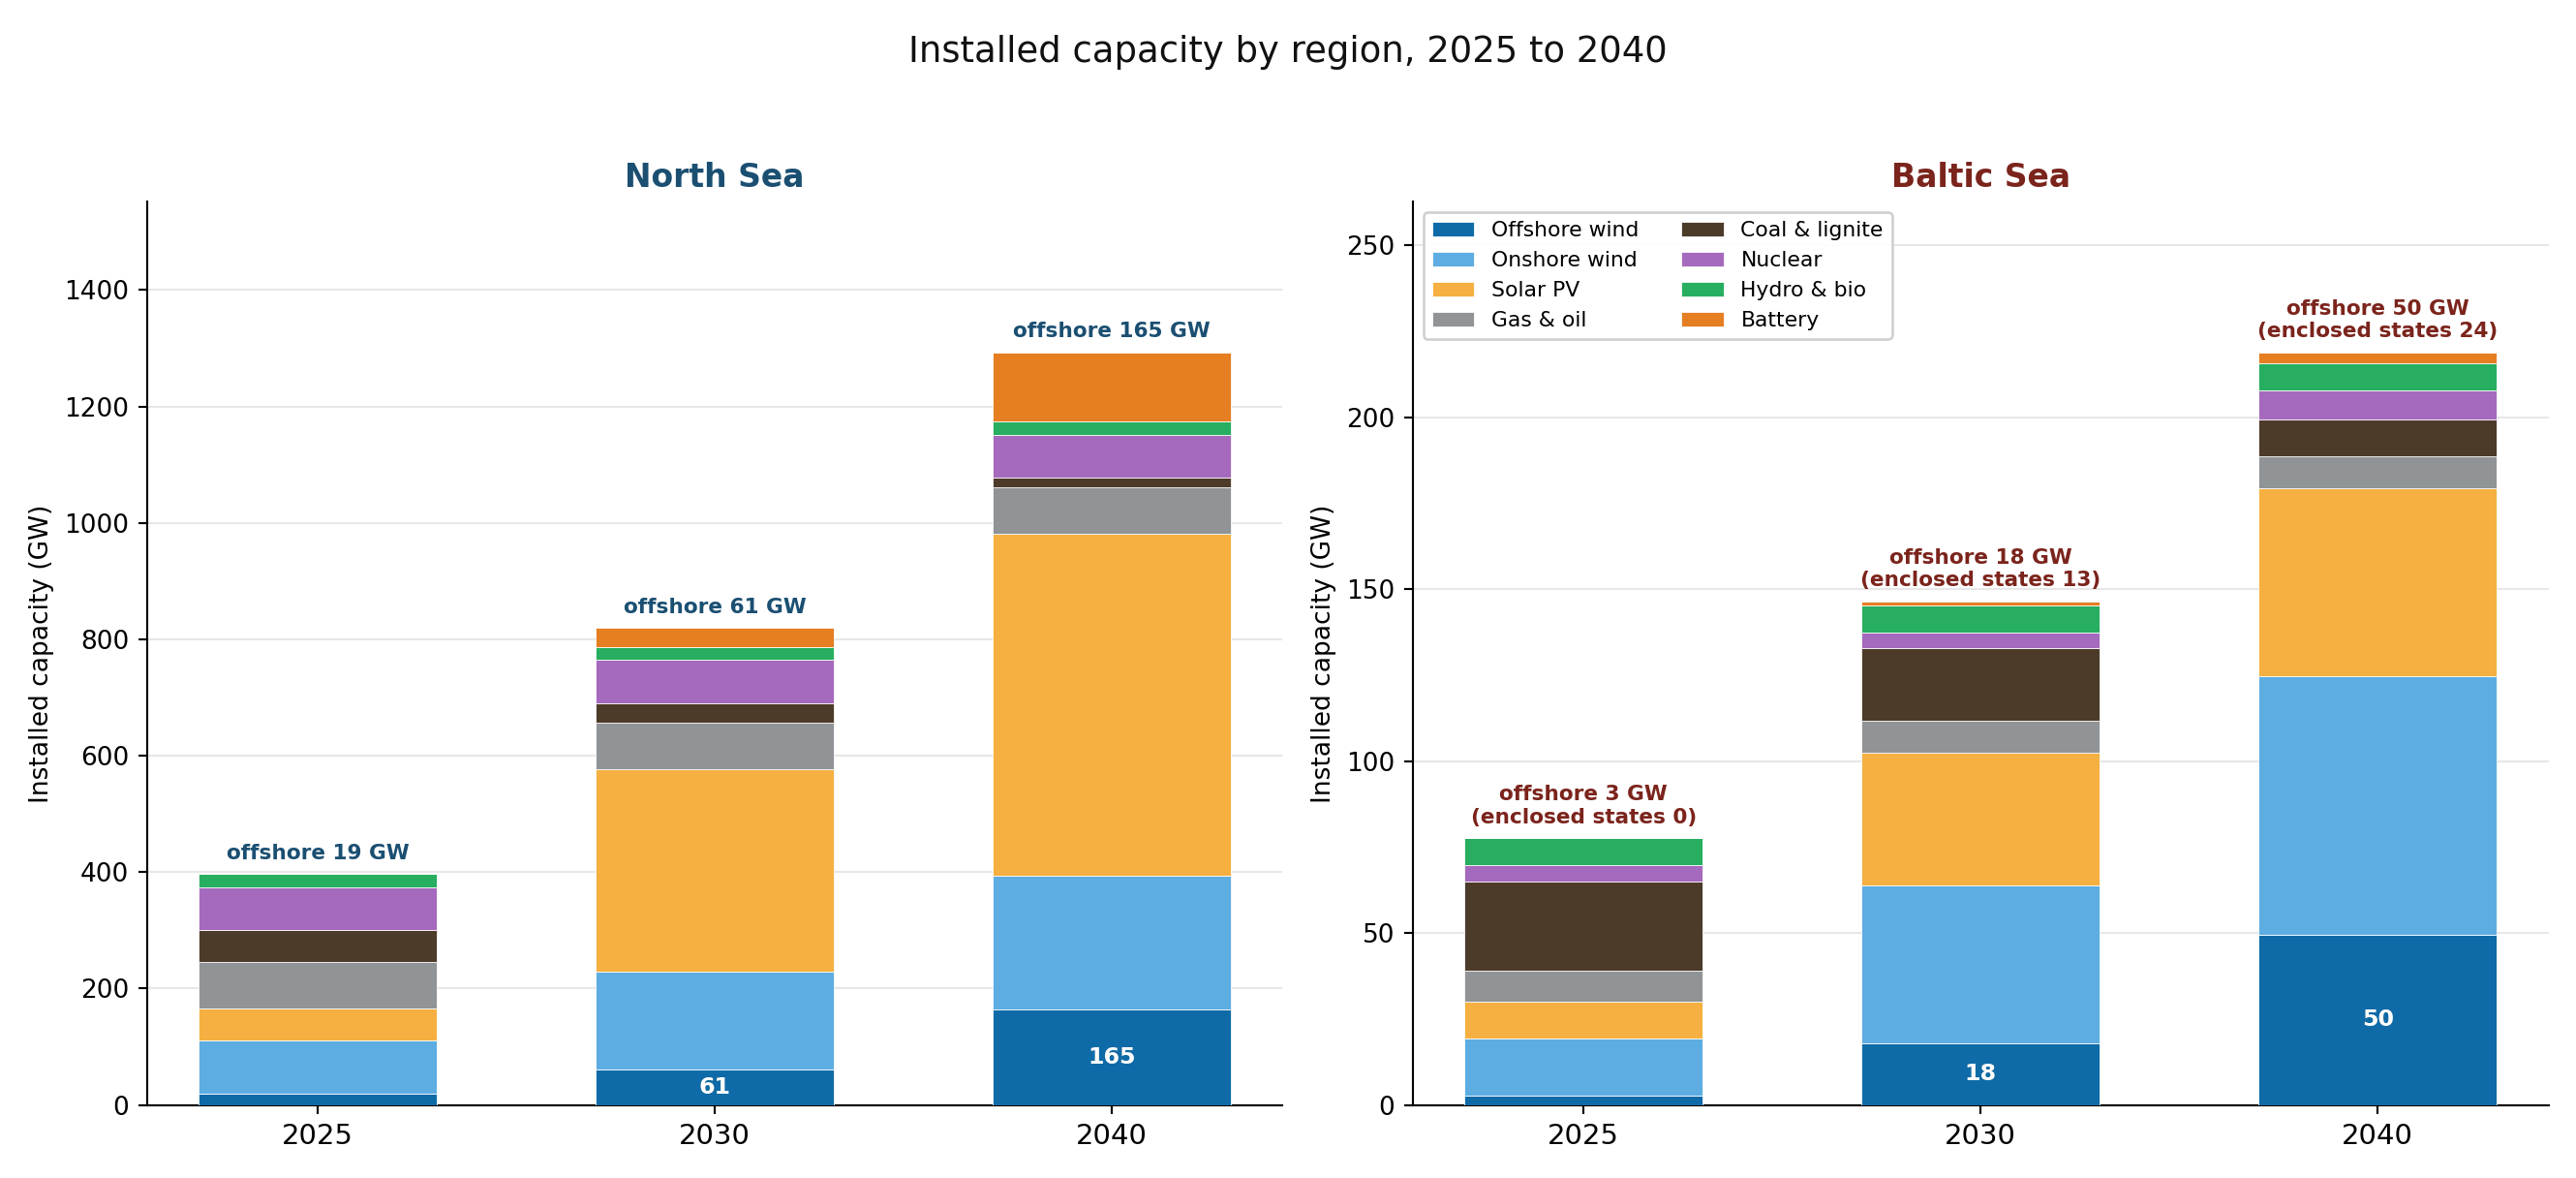
\includegraphics[width=0.95\textwidth]{fig_energy_mix}
    \caption{Installed capacity to 2040 under the TYNDP trajectories. Offshore
    wind is assigned to the sea each farm stands in, and all other capacity to
    the fleet of the bordering region.}
    \label{fig:energy_mix}
\end{figure}

Around the North Sea, offshore wind grows from 18.5 to 164.8~GW, nine times its
present size. Around the Baltic it grows from 2.6 to 49.5~GW, nineteen times its
present size. The Baltic starts much smaller and grows twice as fast, and that
difference drives the results below.

What stays in the system matters as much as what is added. Gas, nuclear and
hydro capacity remain at similar levels in all three years, and only coal
declines. Wind costs almost nothing to run once it is built, so in windy hours
it pushes the wholesale price down. In hours with little wind, gas and other
conventional plants are still needed and still set the price. Capture value
falls because more and more wind output arrives in the hours when wind has
already pushed the price down.
\subsubsection{Projected capture value to 2030 and 2040}\label{sec:corrected_projection}

The system model was solved for six scenarios from the 2024 Ten-Year Network
Development Plan, listed in Table~\ref{tab:projection}. They cover 2030 and
2040, a scheduled and an accelerated pace of Baltic buildout, and the plan's
three demand pathways. National Trends, the pathway that tracks existing
national policies, is the one quoted in the text, and the table gives the
rest. Finland is set aside, as in the measured record.

Baltic capture value falls steeply under National Trends, from 0.88 today to
0.47 by 2040, while the North Sea holds 0.57, and most of the fall arrives
after 2030. The faster the Baltic builds, the further it
falls: in the accelerated case it reaches 0.36. These values come from the
model directly, with no correction applied, and in every 2040 scenario the
Baltic ends below the North Sea.

Applying the correction for the overstatement measured in
Section~\ref{sec:trust_system} (the model reads too high in congested zones)
deepens each 2040 value by roughly a further 0.1. The correction is a
refinement, and the conclusion does not depend on it, since its size rests
almost entirely on DK2, and removing that zone leaves a nearly constant
adjustment (Appendix~\ref{app:robustness}). Where a single number is needed,
this thesis uses 0.47, the uncorrected National Trends case on today's grid,
at which the Baltic has lost close to half of its present value.

Two further checks leave this conclusion unchanged, as expanding the
transmission grid softens the fall without undoing it
(Section~\ref{sec:grid_results}) and the assumed level of hydrogen demand
barely moves it. The basin average also
conceals differences between zones, with Estonia falling furthest and Poland
least (Appendix~\ref{app:tables}), but every zone that builds out loses value.

\begin{table}[!htb]
\centering\small
\caption{Projected capture value by scenario, averaged across each basin and
weighted by generation, from the system model with the transmission grid held
at today's capacity and no correction applied. The corrected Baltic values are
in Appendix~\ref{app:robustness}; Finland is set aside throughout.}
\label{tab:projection}
\begin{tabular}{c l l c c c}
\toprule
\textbf{Year} & \textbf{Demand pathway} & \textbf{Baltic buildout} &
\textbf{Baltic offshore} & \textbf{North Sea} & \textbf{Baltic} \\
 & & & \textbf{share of consumption} & \textbf{capture value} &
\textbf{capture value} \\
\midrule
2030 & National Trends & scheduled & 0.24 & 0.84 & 0.79 \\
2030 & National Trends & accelerated & 0.29 & 0.84 & 0.75 \\
\addlinespace
2040 & National Trends & scheduled & 0.33 & 0.57 & 0.47 \\
2040 & National Trends & accelerated & 0.51 & 0.57 & 0.36 \\
2040 & Distributed Energy & accelerated & 0.38 & 0.63 & 0.60 \\
2040 & Global Ambition & accelerated & 0.40 & 0.70 & 0.57 \\
\bottomrule
\end{tabular}
\end{table}
\subsubsection{Spatial distribution of projected capture value}\label{sec:maps}

Figure~\ref{fig:heatmap_2040} shows the capture value a farm would earn at each
buildable location in 2040. The 2025 and 2030 maps are in
Appendix~\ref{app:reg_tables}.

\begin{figure}[!htb]
    \centering
    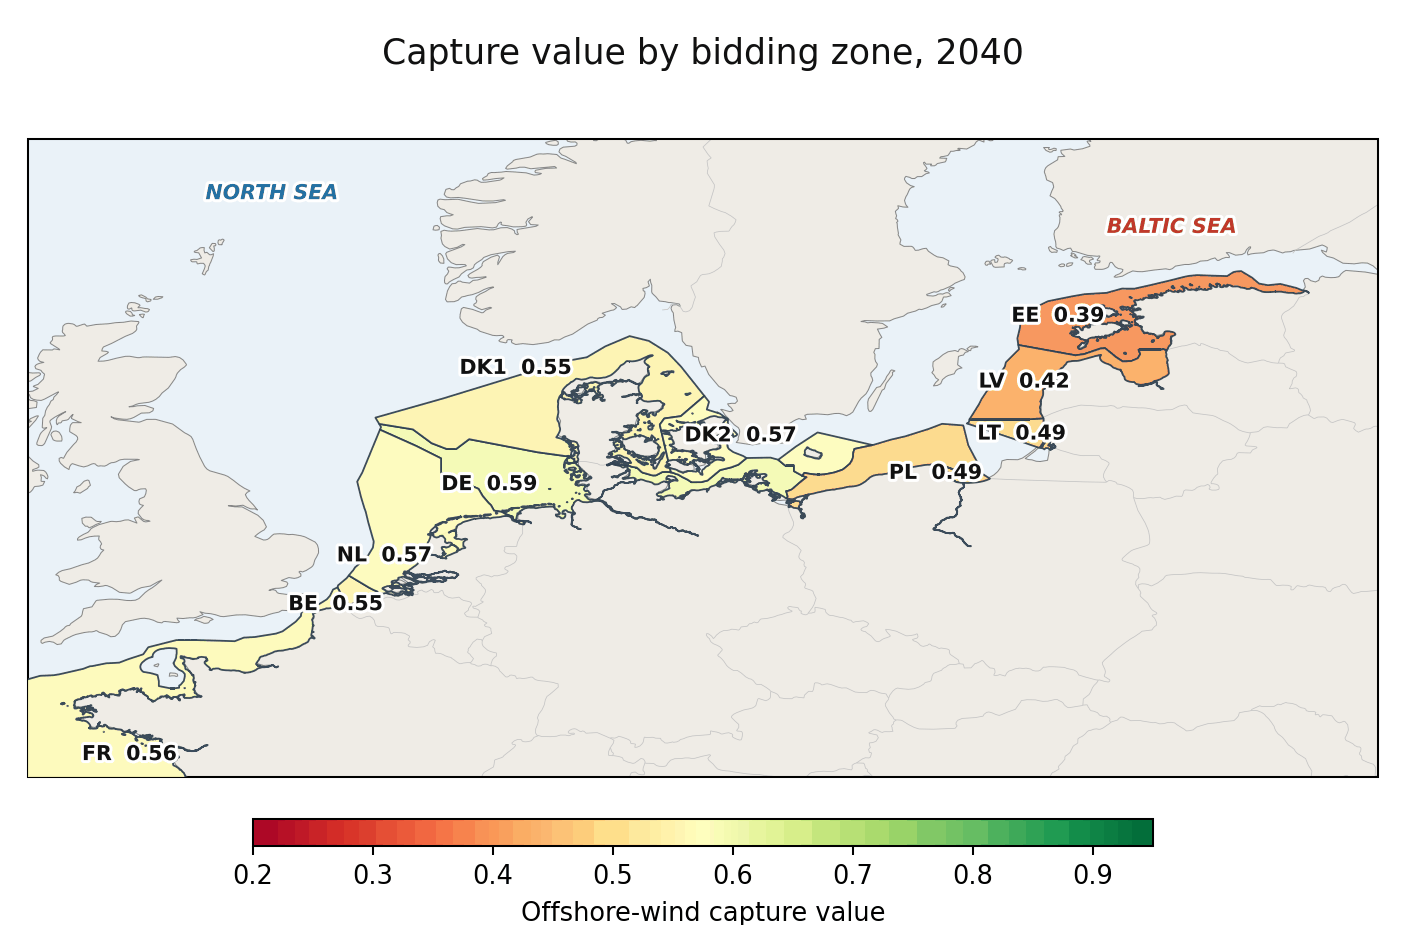
\includegraphics[width=0.80\textwidth]{fig_heatmap_2040}
    \caption{Capture value at each buildable location in 2040, with the
    transmission grid held at today's capacity. The North Sea holds close to its
    present level, while the enclosed eastern Baltic falls furthest.}
    \label{fig:heatmap_2040}
\end{figure}

In 2025 capture value is high and much the same across the whole shelf. By 2030
it has fallen everywhere, with no clear difference between the two seas. By 2040
the two have separated: the eastern Baltic is lowest, while the North Sea holds
its level despite taking far more new capacity. What decides the fall is how
easily a basin can move its surplus away.

Appendix~\ref{app:atlas} repeats these maps under cost-optimal transmission,
alongside levelised cost, value-adjusted cost, net value and revenue density at
all three years. Comparing the frozen and expanded versions shows the split of
Section~\ref{sec:decomposition} geographically.
\FloatBarrier


% ----------------------------------------------------------------------------
\FloatBarrier
\subsection{Drivers of value erosion and its recoverable component}\label{sec:mechanism}

This section examines what drives the fall in capture value and how much of it
depends on the configuration of the surrounding system. The first part
identifies what sets the severity of the fall: the differences between
individual farms, the shape of the relationship between buildout and value,
and the season in which the loss concentrates. The second part quantifies that
dependence, by re-solving the scenarios with transmission free to expand and
by decomposing the fall into a congestion component and a structural
component.

Three further checks are reported in Appendix~\ref{app:robustness}. The same
geography appears from hourly generation alone, with no prices used at all.
Removing the hours priced by scarcity leaves the fall largely intact. And
allowing demand to shift in time recovers as much capture value as expanding the
grid does.

\subsubsection{Farm-level drivers}\label{sec:shap_results}

This part asks why one farm earns less than another in the same month. Carbon
and gas prices cannot explain it: they are Europe-wide monthly prices, identical
in every zone, so they move all farms together. They still appear important in
the fitted model, because the 2021 to 2022 fuel crisis moved fuel prices and
capture value at the same time.

Comparing each farm with the average of all farms in the same month removes that
common movement (Figure~\ref{fig:shap}). Carbon's share then falls from 29 to
4\,\% and gas from 14 to 3\,\%. Crowding takes their place: how closely a farm's
output follows the wind of the system around it explains 32\,\% on its own, and
the zone's existing wind capacity a further 13\,\%. A farm generating when
everything else is generating sells into a market already full of wind, and that
is the largest single cause of a low capture value.

The rest is the system's ability to absorb that surplus. How well demand matches
generation, how much flexibility exists, and how much can be exported together
explain about 48\,\%, each by moving surplus out of the windiest hours, either
across a border or into storage. The Baltic, with less export
capacity, is the more exposed basin. Fuel prices still set the overall price
level, but the differences between farms come from crowding and from how much
surplus the system can absorb.

\begin{figure}[!htb]
    \centering
    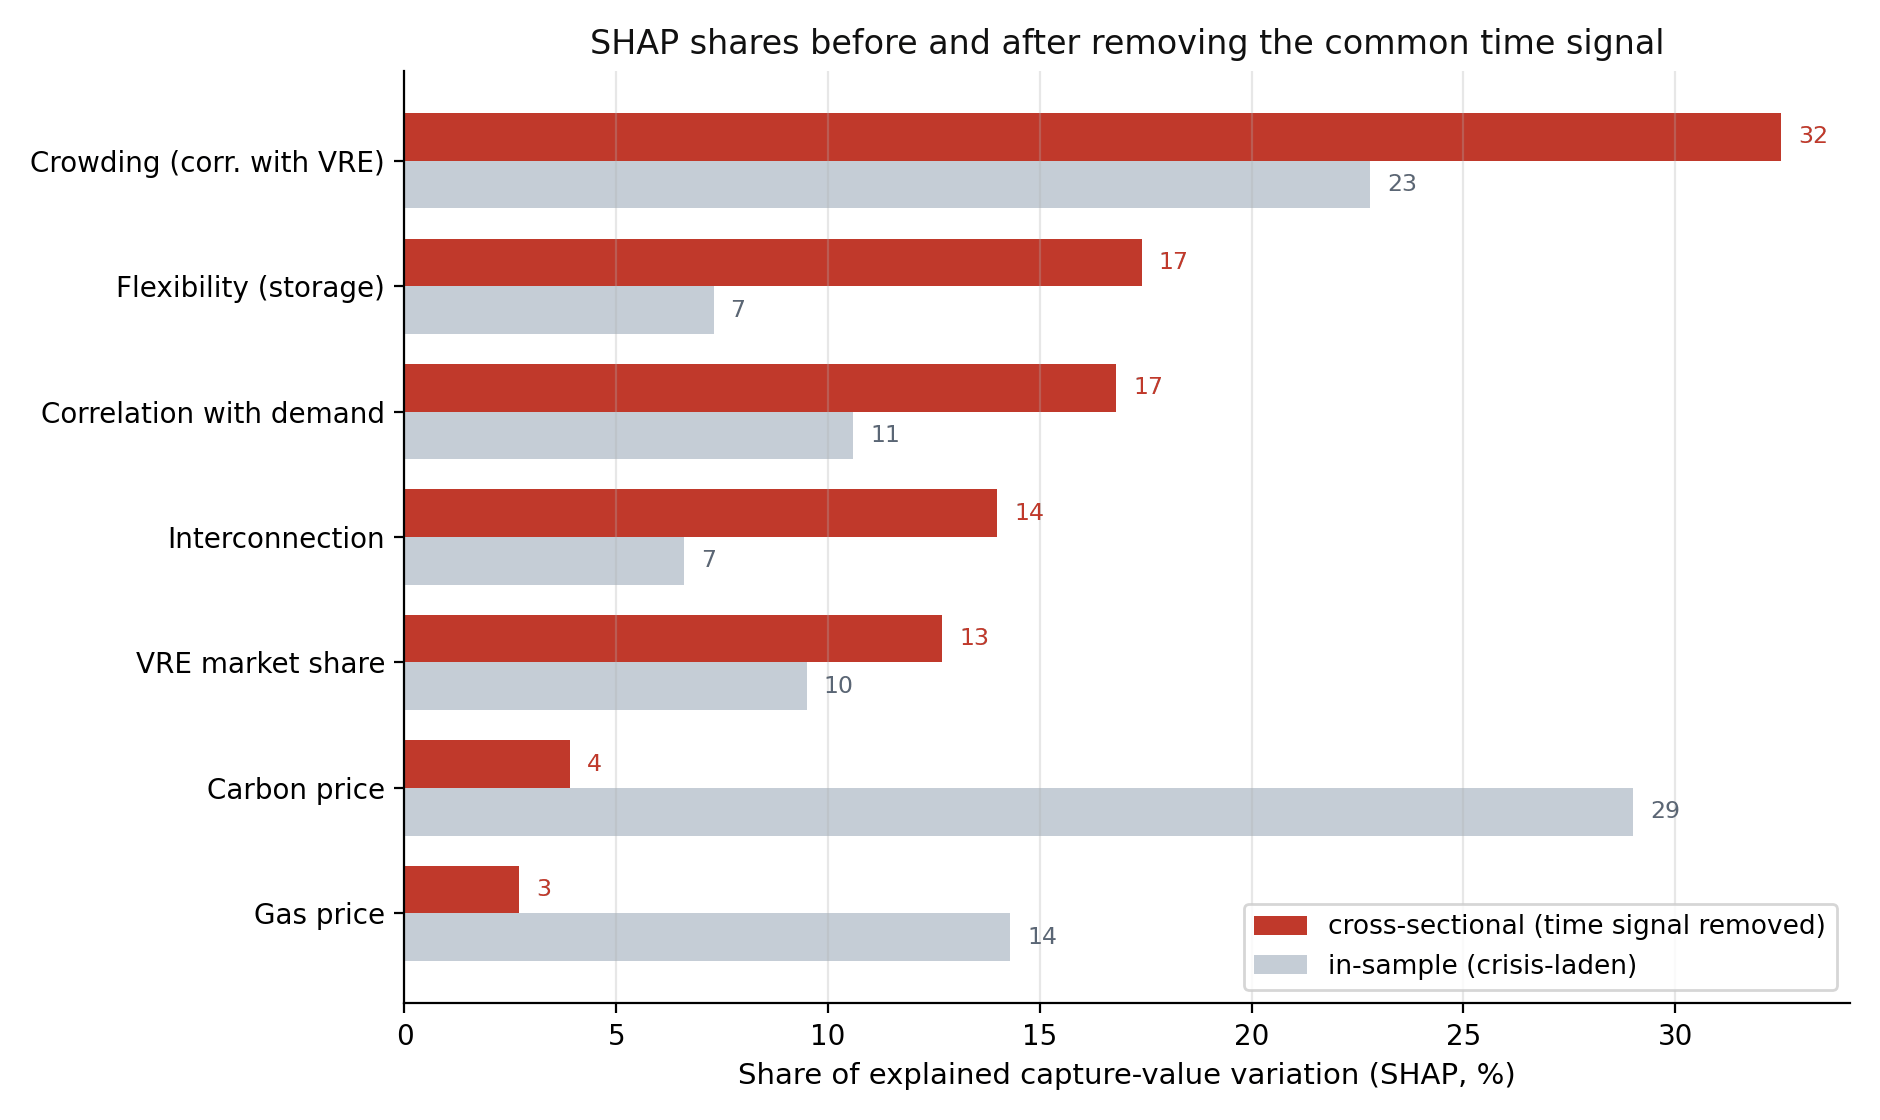
\includegraphics[width=0.95\textwidth]{fig_shap_demeaned}
    \caption{Importance of each driver of capture value, measured by SHAP.
    Grey shows the values as fitted; red shows them after each farm is
    compared with the average of all farms in the same month, which removes
    movements common to every zone.}
    \label{fig:shap}
\end{figure}

A much simpler equation, fitted separately to each basin, checks this result
(Equation~\ref{eq:analytical}). One term in it measures how heavily a farm is
penalised for generating at the same time as everything else. That penalty is
0.74 in the Baltic against 0.37 in the North Sea, and the Baltic is the steeper
of the two in 99 of 100 resamplings of the farms. Capture value falls
about 1.6 times as fast per unit of buildout in the Baltic as in the North Sea
today, and about 1.9 times as fast once wind dominates the system. Fifteen farms
is a small basis, so this is indicative, but it agrees with the system model,
which shows a moderate fall by 2030 and a severe one by 2040. The fit is in
Appendix~\ref{app:analytical}\label{sec:one_equation}.
\subsubsection{Seasonality of the erosion}\label{sec:seasonality}

Wind in the two basins peaks together in winter and separate in summer
(Figure~\ref{fig:crossbasin_sync}). Their output moves together at a correlation
near 0.4 in winter, falling to 0.13 in July. The Baltic can therefore export its
surplus in summer, but not in winter, when the same Atlantic weather reaches
both seas. Export capacity is least useful in the season when output is highest.

\begin{figure}[!htb]
    \centering
    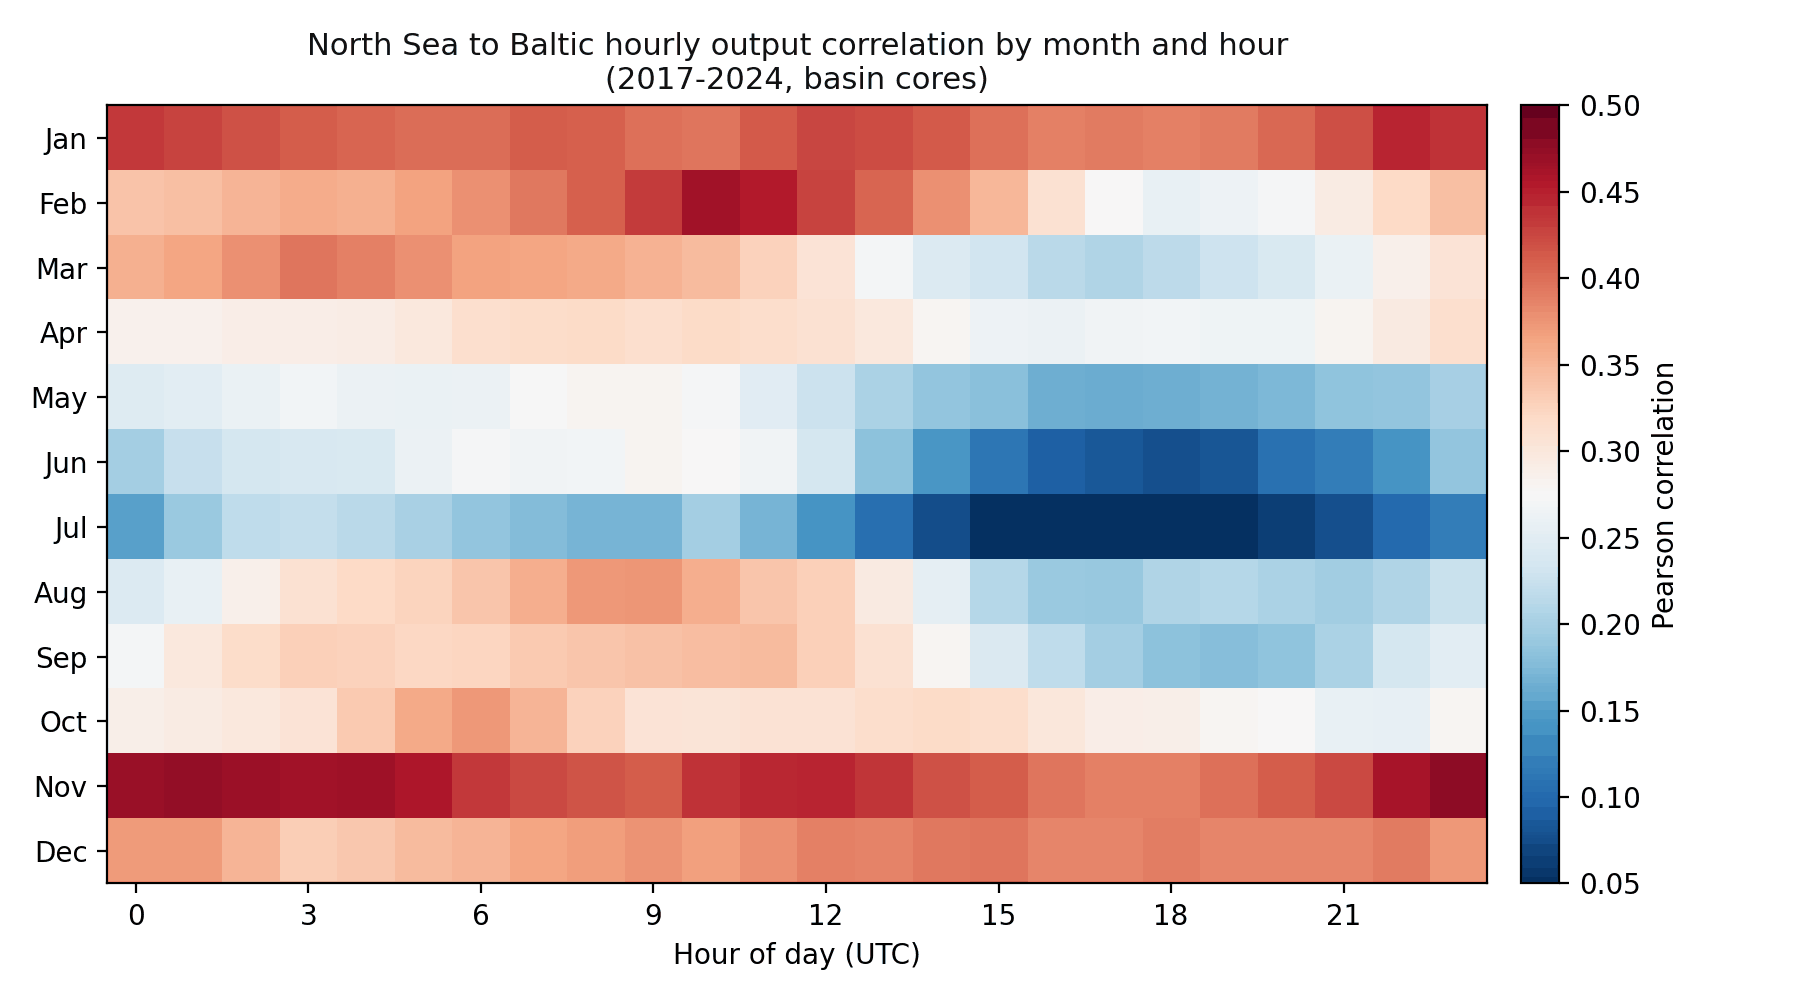
\includegraphics[width=0.95\textwidth]{fig_crossbasin_sync}
    \caption{How closely wind output in the two basins moves together, by month
    and hour, 2017 to 2024. The correlation averages 0.38 in winter and 0.20 in
    summer, and is lowest on summer afternoons.}
    \label{fig:crossbasin_sync}
\end{figure}

That matters because winter is when the farms generate, at about 70\,\% of
capacity against 40\,\% in summer, yet today they record the same capture value
in both seasons. By 2040 the loss falls almost entirely in winter, to 0.56 in the
North Sea and 0.50 in the Baltic, while summer stays at 0.91 and 0.83
(Figure~\ref{fig:seasonal_generation}, Appendix~\ref{app:supplementary}). Most
of the year's output arrives in winter, so the winter fall is what produces the
annual one, and any remedy must work in that season: interconnection, seasonal
storage, or demand that can shift into windy winter hours.

\subsubsection{The effect of transmission expansion}
\label{sec:grid_results}

The projection so far holds the grid at today's capacity, which is a
pessimistic assumption, since transmission will be built over the fifteen
years to 2040. To find the opposite bound, all six scenarios were solved again
with transmission free to expand wherever doing so lowers total system cost
(Figure~\ref{fig:grid_bracket}).

Expansion changes nothing at 2030, because the congestion it would relieve has
not yet appeared. By 2040 it matters a great deal. Under National Trends the
Baltic recovers from 0.47 to 0.66 while the North Sea moves from 0.57 to 0.64,
so the basin that trails on today's grid ends slightly ahead once the grid is
expanded. Every Baltic zone shares in the gain, Poland most of all. 

Two conclusions follow from this comparison: the Baltic's disadvantage
relative to the North Sea is largely attributable to congestion and disappears
once transmission is expanded, whereas its loss relative to its own present
value persists under either grid assumption, since the fall from 0.88 today is
severe in both.

\begin{figure}[H]
    \centering
    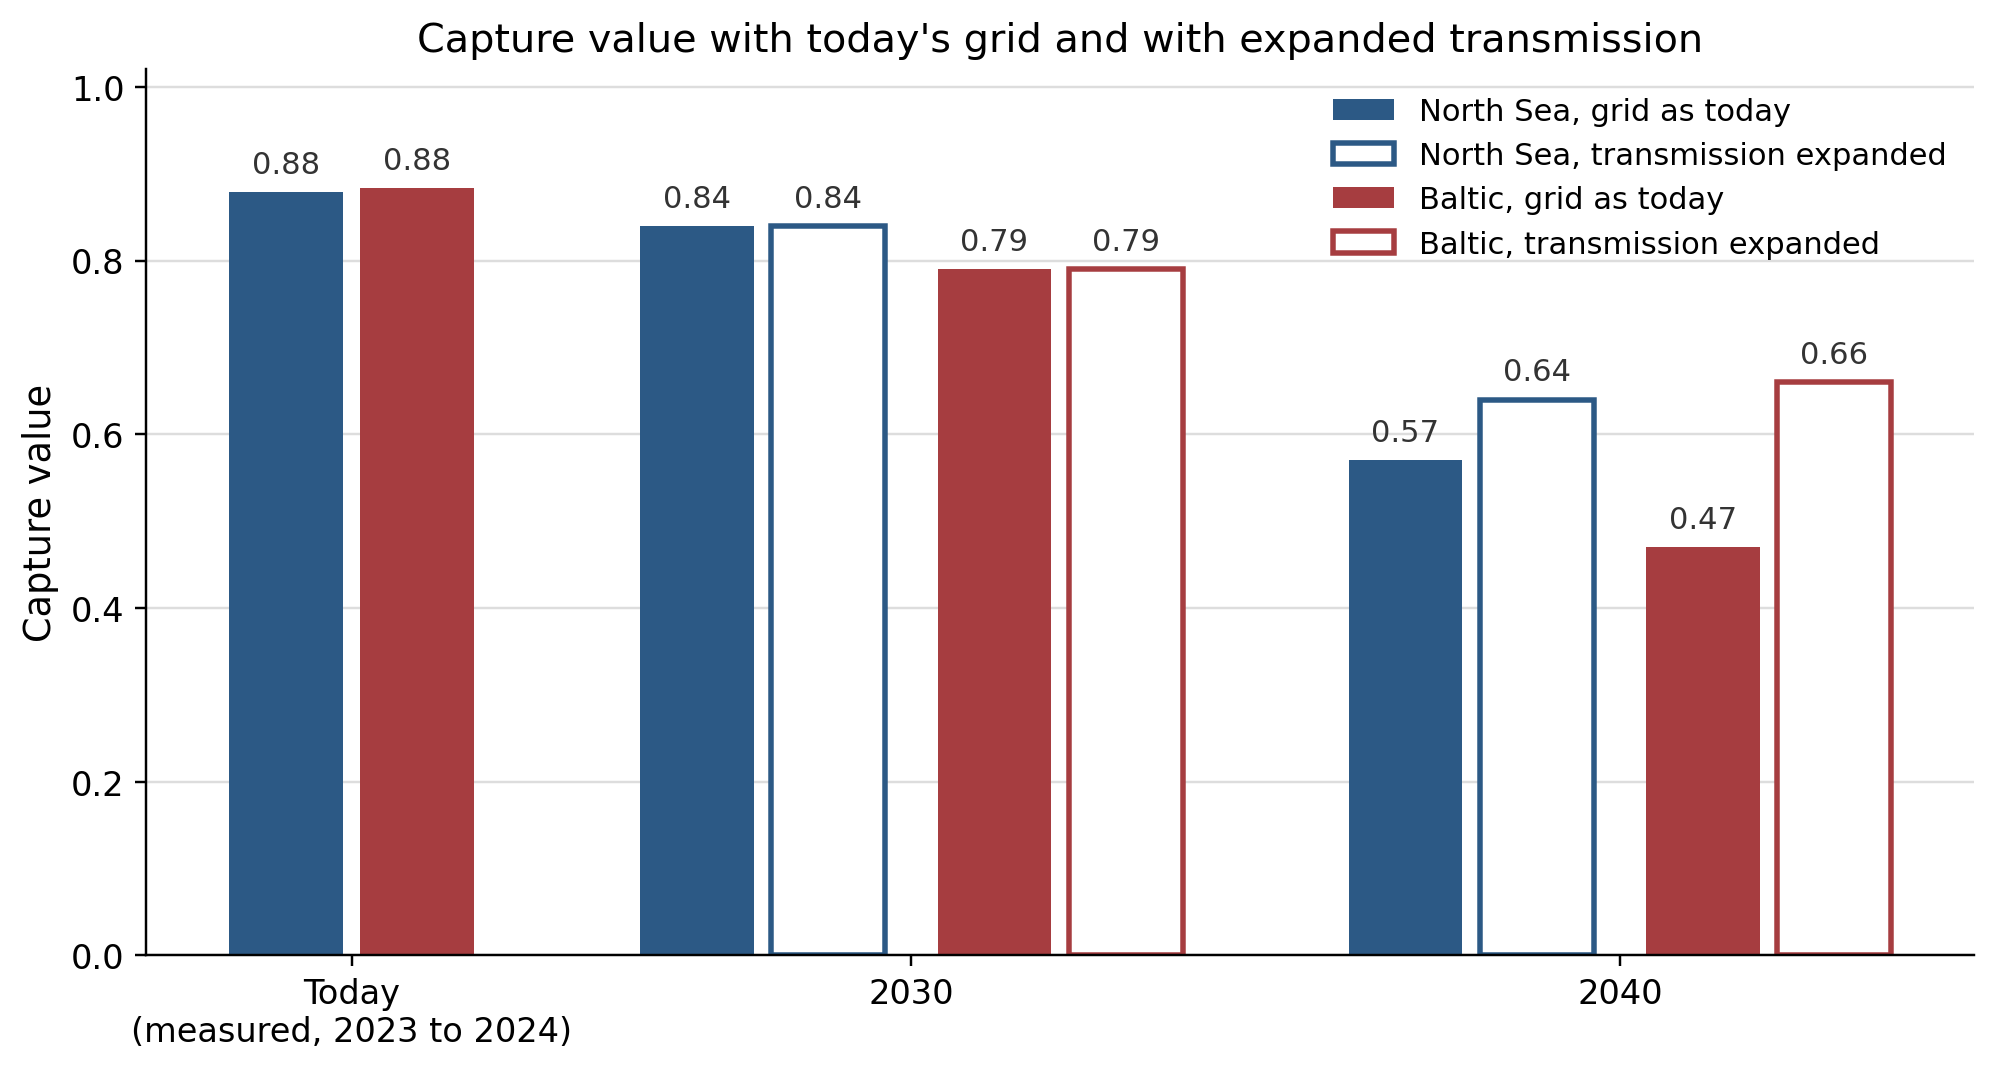
\includegraphics[width=0.9\textwidth]{figures/image-1787752046559.png}
    \caption{Capture value in both basins with the grid held at today's
    capacity and with transmission free to expand, under National Trends with
    the scheduled buildout. The bars for today are the measured 2023 to 2024
    values, where only one grid exists. Expansion makes no difference in 2030,
    and by 2040 it lifts both basins, the Baltic by more, because its loss is
    mostly congestion. Values are from the model before the bias correction,
    which is applied in the text.}
    \label{fig:grid_bracket}
\end{figure}

\subsubsection{Decomposition into congestion and structural components}\label{sec:decomposition}

The previous section establishes that transmission expansion matters, but it
does not establish how much of the total fall congestion accounts for. That
share is the number the policy conclusion rests on, because the congestion
part of the fall can be removed by building lines, while the part caused by
the buildout itself remains whatever is built.

The two model runs already provide this separation, since today's observed
capture value is the starting point, the run with transmission free to expand
gives the value a basin would hold if the grid were never a constraint, and
the run with the grid frozen gives the value it holds now. The fall between today and 2040 therefore divides
in two:
%
\begin{equation}
    \underbrace{\mathrm{CV}_{\text{today}} - \mathrm{CV}_{\text{frozen}}}_{\text{total fall}}
    = \underbrace{\bigl(\mathrm{CV}_{\text{today}} - \mathrm{CV}_{\text{optimal}}\bigr)}_{\text{structural, which no grid removes}}
    + \underbrace{\bigl(\mathrm{CV}_{\text{optimal}} - \mathrm{CV}_{\text{frozen}}\bigr)}_{\text{congestion, which an expanded grid removes}}
    \label{eq:cv_decomposition}
\end{equation}

Both basins start level, at 0.887 in the North Sea and 0.889 in the Baltic,
within half a point of the measured 0.879 and 0.883. By 2040 on the frozen grid
the North Sea has fallen by 0.314 and the Baltic by 0.418. Of the North Sea's
fall, 0.250 is structural and 0.064 is congestion, a split of 80 to 20. Of the
Baltic's, 0.225 is structural and 0.193 is congestion, a split of 54 to 46
(Figure~\ref{fig:cv_decomposition}).

\begin{figure}[!htb]
    \centering
    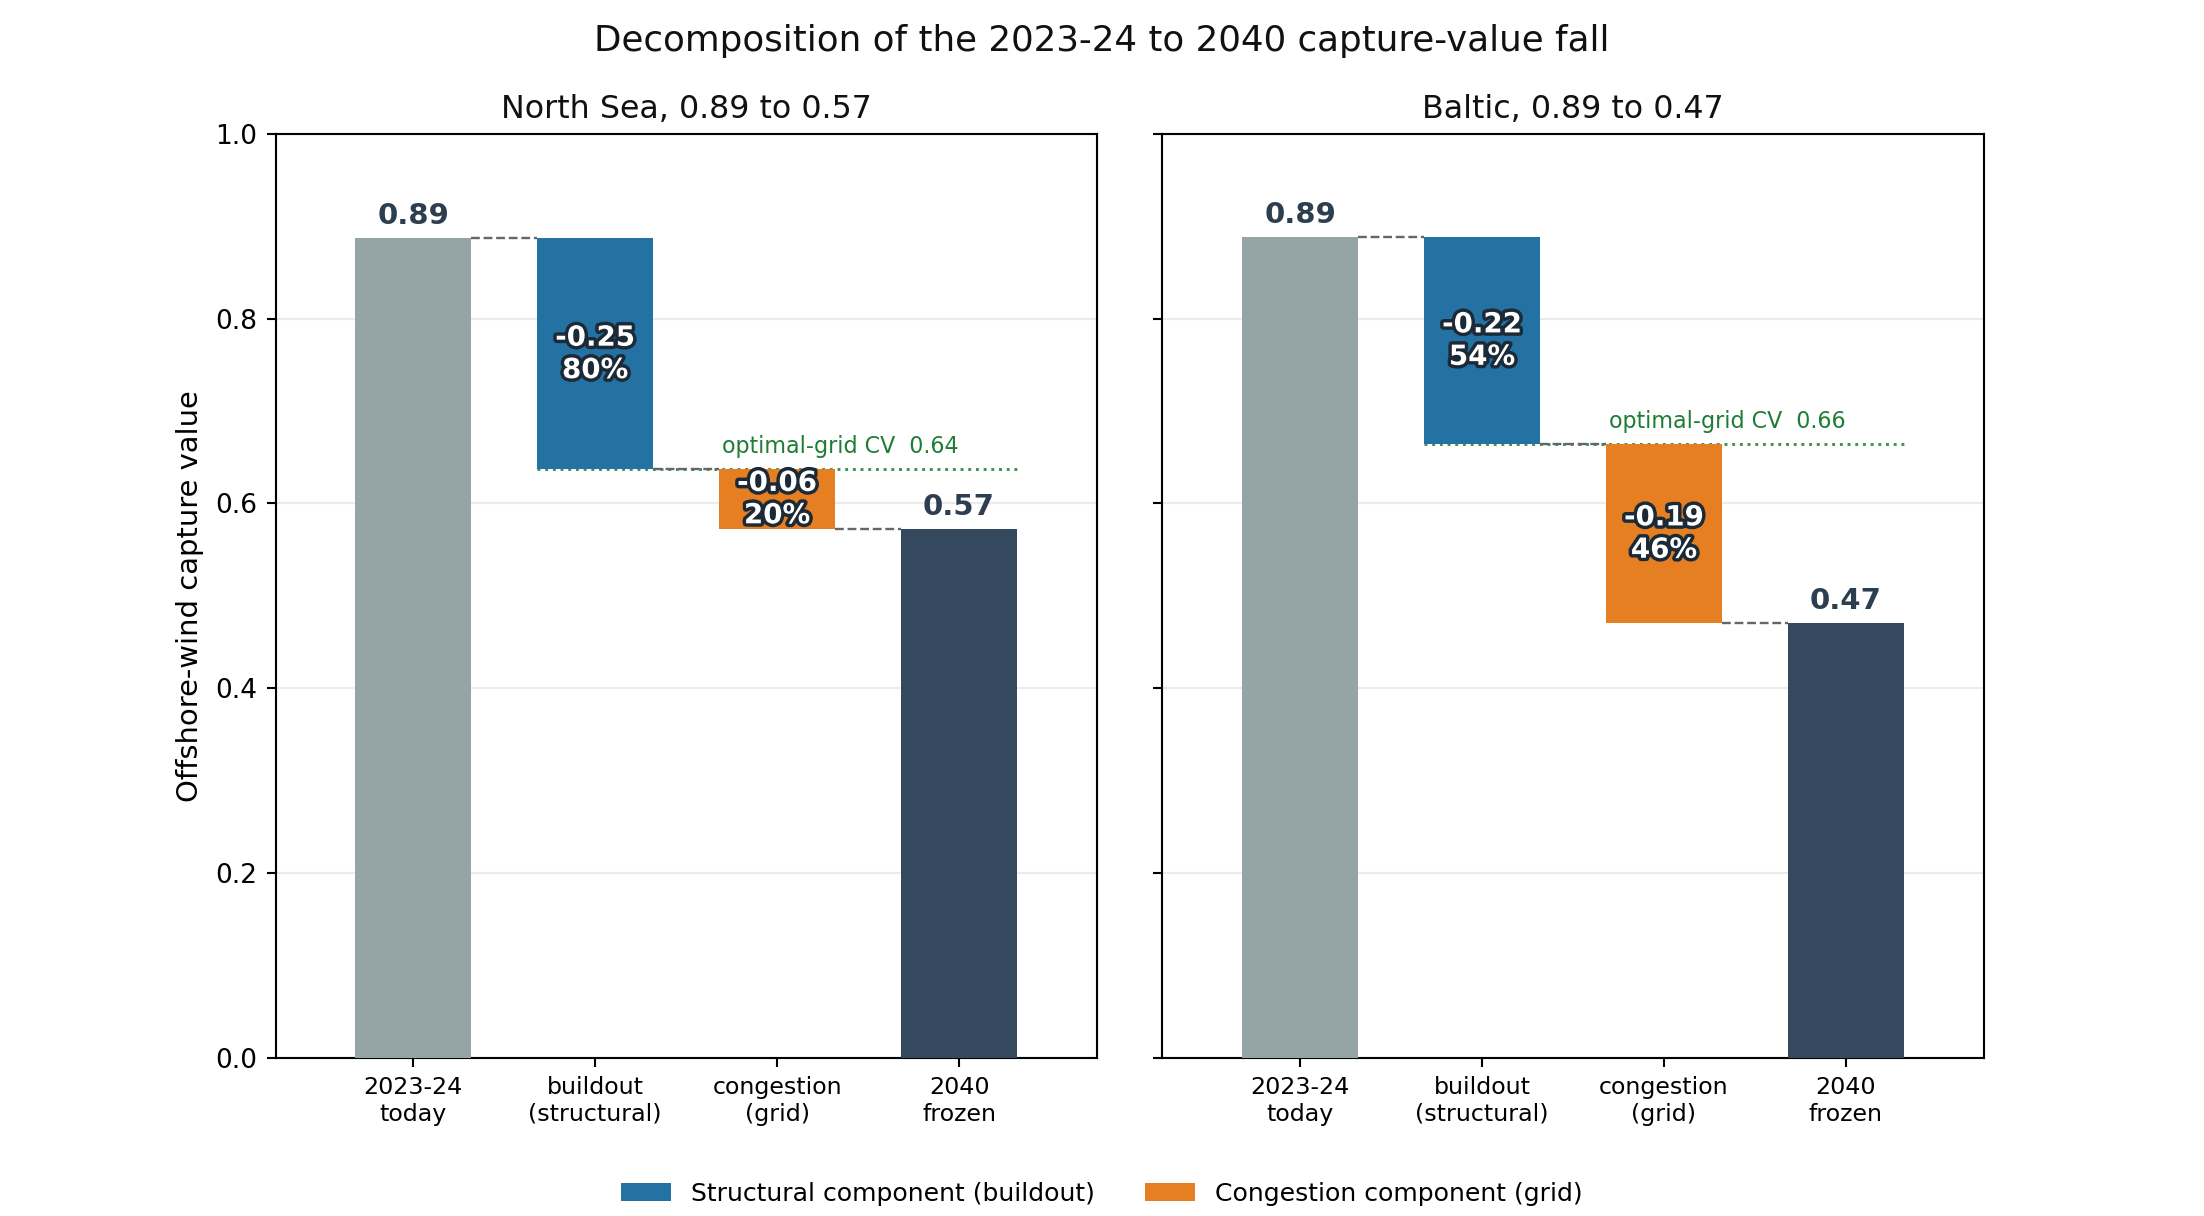
\includegraphics[width=0.94\textwidth]{fig_cv_decomposition}
    \caption{Each basin's fall in capture value between today and 2040, divided
    into the part caused by the buildout itself, which no amount of transmission
    removes, and the part caused by congestion, which an expanded grid removes.
    Both basins start at about 0.89.}
    \label{fig:cv_decomposition}
\end{figure}

The Baltic's congestion penalty is three times the North Sea's, which is what an
enclosed basin should show. The more surprising result is the structural fall:
at 0.225 against the North Sea's 0.250, the part no transmission can recover is
the smaller of the two. The share of the Baltic's disadvantage that appears to
come from enclosure is congestion, and congestion is decided by what
is built. How the two components differ in who pays for them, while they remain,
is taken up in Section~\ref{sec:whopays_results}.

\subsection{Value-adjusted cost of energy and site selection}\label{sec:vlcoe_results}

The chapter has measured capture value and explained why it falls. This section
turns it into the number an investor uses. Combining capture value with the
levelised cost of energy (Equation~\ref{eq:vlcoe}) gives the average wholesale
price a site must earn over its life to break even, and that price is mapped
across both basins at the same resolution as the wind and seabed data.

\subsubsection{Levelised cost and the break-even price}\label{sec:vlcoe_paradox}

Building offshore wind is getting cheaper. Across the seabed where farms could
be built, the median levelised cost falls from 74 to 66~\euro/MWh between 2025
and 2040. The price a site must earn to break even moves the other way, rising
from 87 to 121~\euro/MWh (Figure~\ref{fig:vlcoe}), because capture value falls
faster than cost does. The share of that seabed clearing a market price near
70~\euro/MWh falls from about 35 per cent to under 1 per cent.

Cheaper turbines do not save the economics, because offshore wind keeps
improving when measured per megawatt-hour produced, yet gets worse when
measured per megawatt-hour of value delivered, and it is the second that a
merchant project, one selling at market prices without a support contract, is
paid for.

\begin{figure}[!htb]
    \centering
    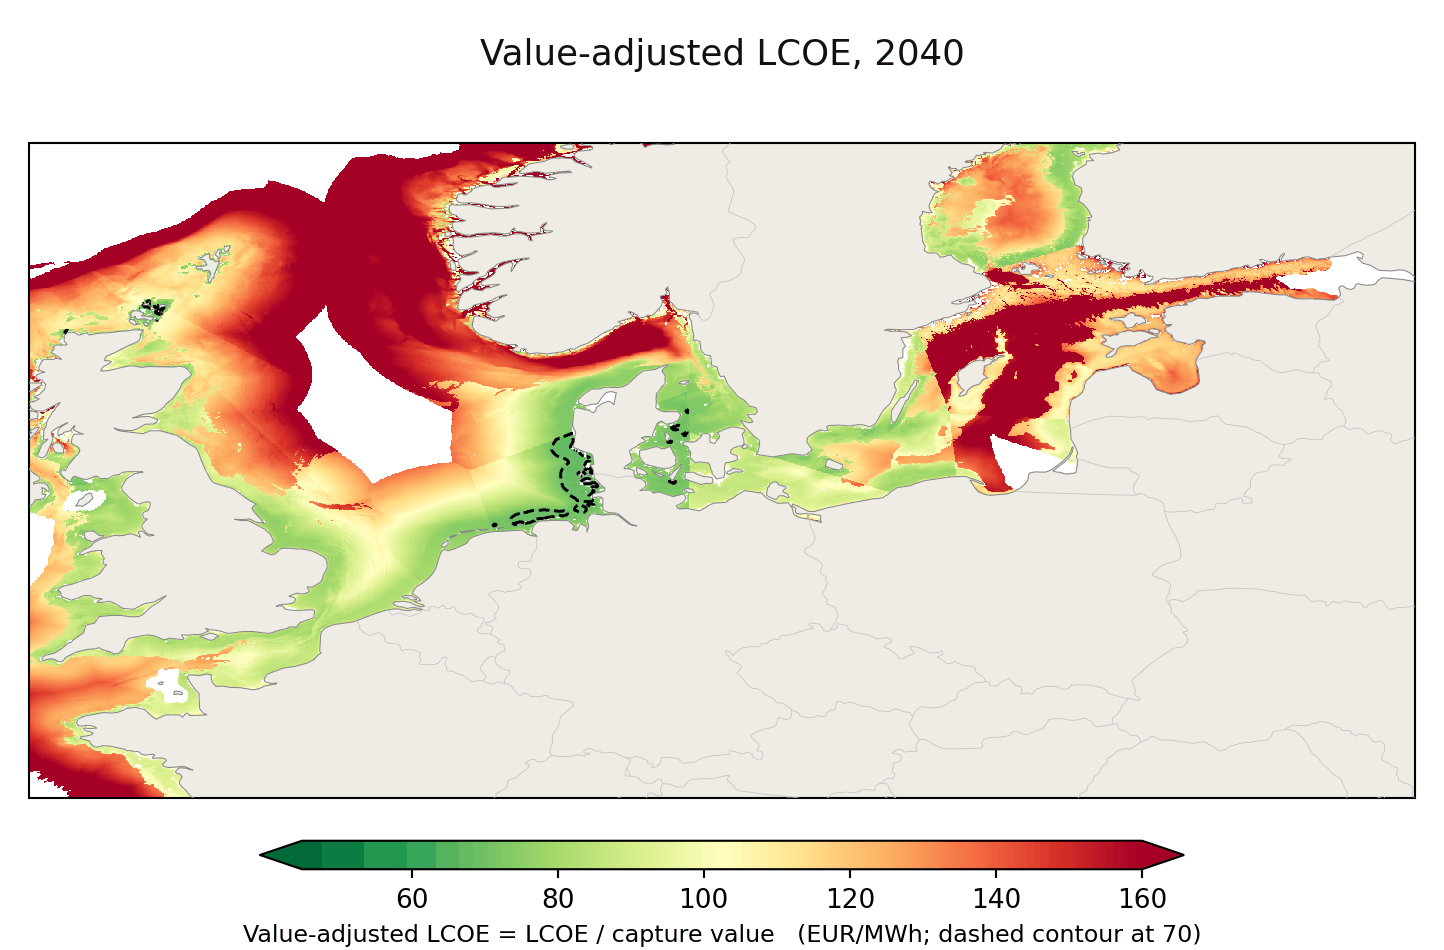
\includegraphics[width=0.6\textwidth]{fig_vlcoe_2040}
    \caption{The average wholesale price each site must earn to break even in
    2040, calculated as levelised cost divided by capture value. The dashed
    contour marks a market price of about 70~\euro/MWh; sites inside it are
    viable at that price.}
    \label{fig:vlcoe}
\end{figure}

The direction does not depend on the cost assumptions. Across all 27
combinations of discount rate, capital cost and learning rate, the break-even
price rises to 2040 in every case (Figure~\ref{fig:vlcoe_robust}). The reason is
that the cost level cancels out: the break-even price is cost divided by capture
value, so what decides the direction is only whether cost falls faster than
value. For the break-even price to stay level, offshore capital costs would have
to fall by about 36 per cent by 2040, three times what the cost database
projects.

Comparing the revenue a farm captures against its annual cost gives the same
picture in absolute terms\label{sec:netvalue_results}. About 48 per cent of the
buildable seabed is profitable at market prices in 2025, and roughly 12 per cent
by 2040. Falling value drives that shrinkage, since costs are falling over the
same period (Appendix~\ref{app:atlas}).

\subsubsection{Monetised value of interconnection}\label{sec:vlcoe_grid_results}

The break-even price is levelised cost divided by capture value, so the grid
result of Section~\ref{sec:grid_results} reappears in terms of money. The 2040
break-even price was recalculated with the frozen and the expanded capture
values, holding offshore cost identical in both. Expansion lowers it everywhere,
and four times more in the enclosed Baltic than in the open North Sea: by about
8~\euro/MWh in the North Sea, by 33 in the enclosed Baltic, and by 48 in the
Danish corridor that carries the redirected flows
(Figure~\ref{fig:vlcoe_grid}).

In revenue terms the Baltic gain alone is worth roughly 1.2 billion euros a
year, close to half the annual cost of the whole transmission programme, and
that is before the congestion rent of Section~\ref{sec:rent_results} is counted.
Interconnection therefore cuts the break-even price where the cut is most
needed.

\begin{figure}[!htb]
    \centering
    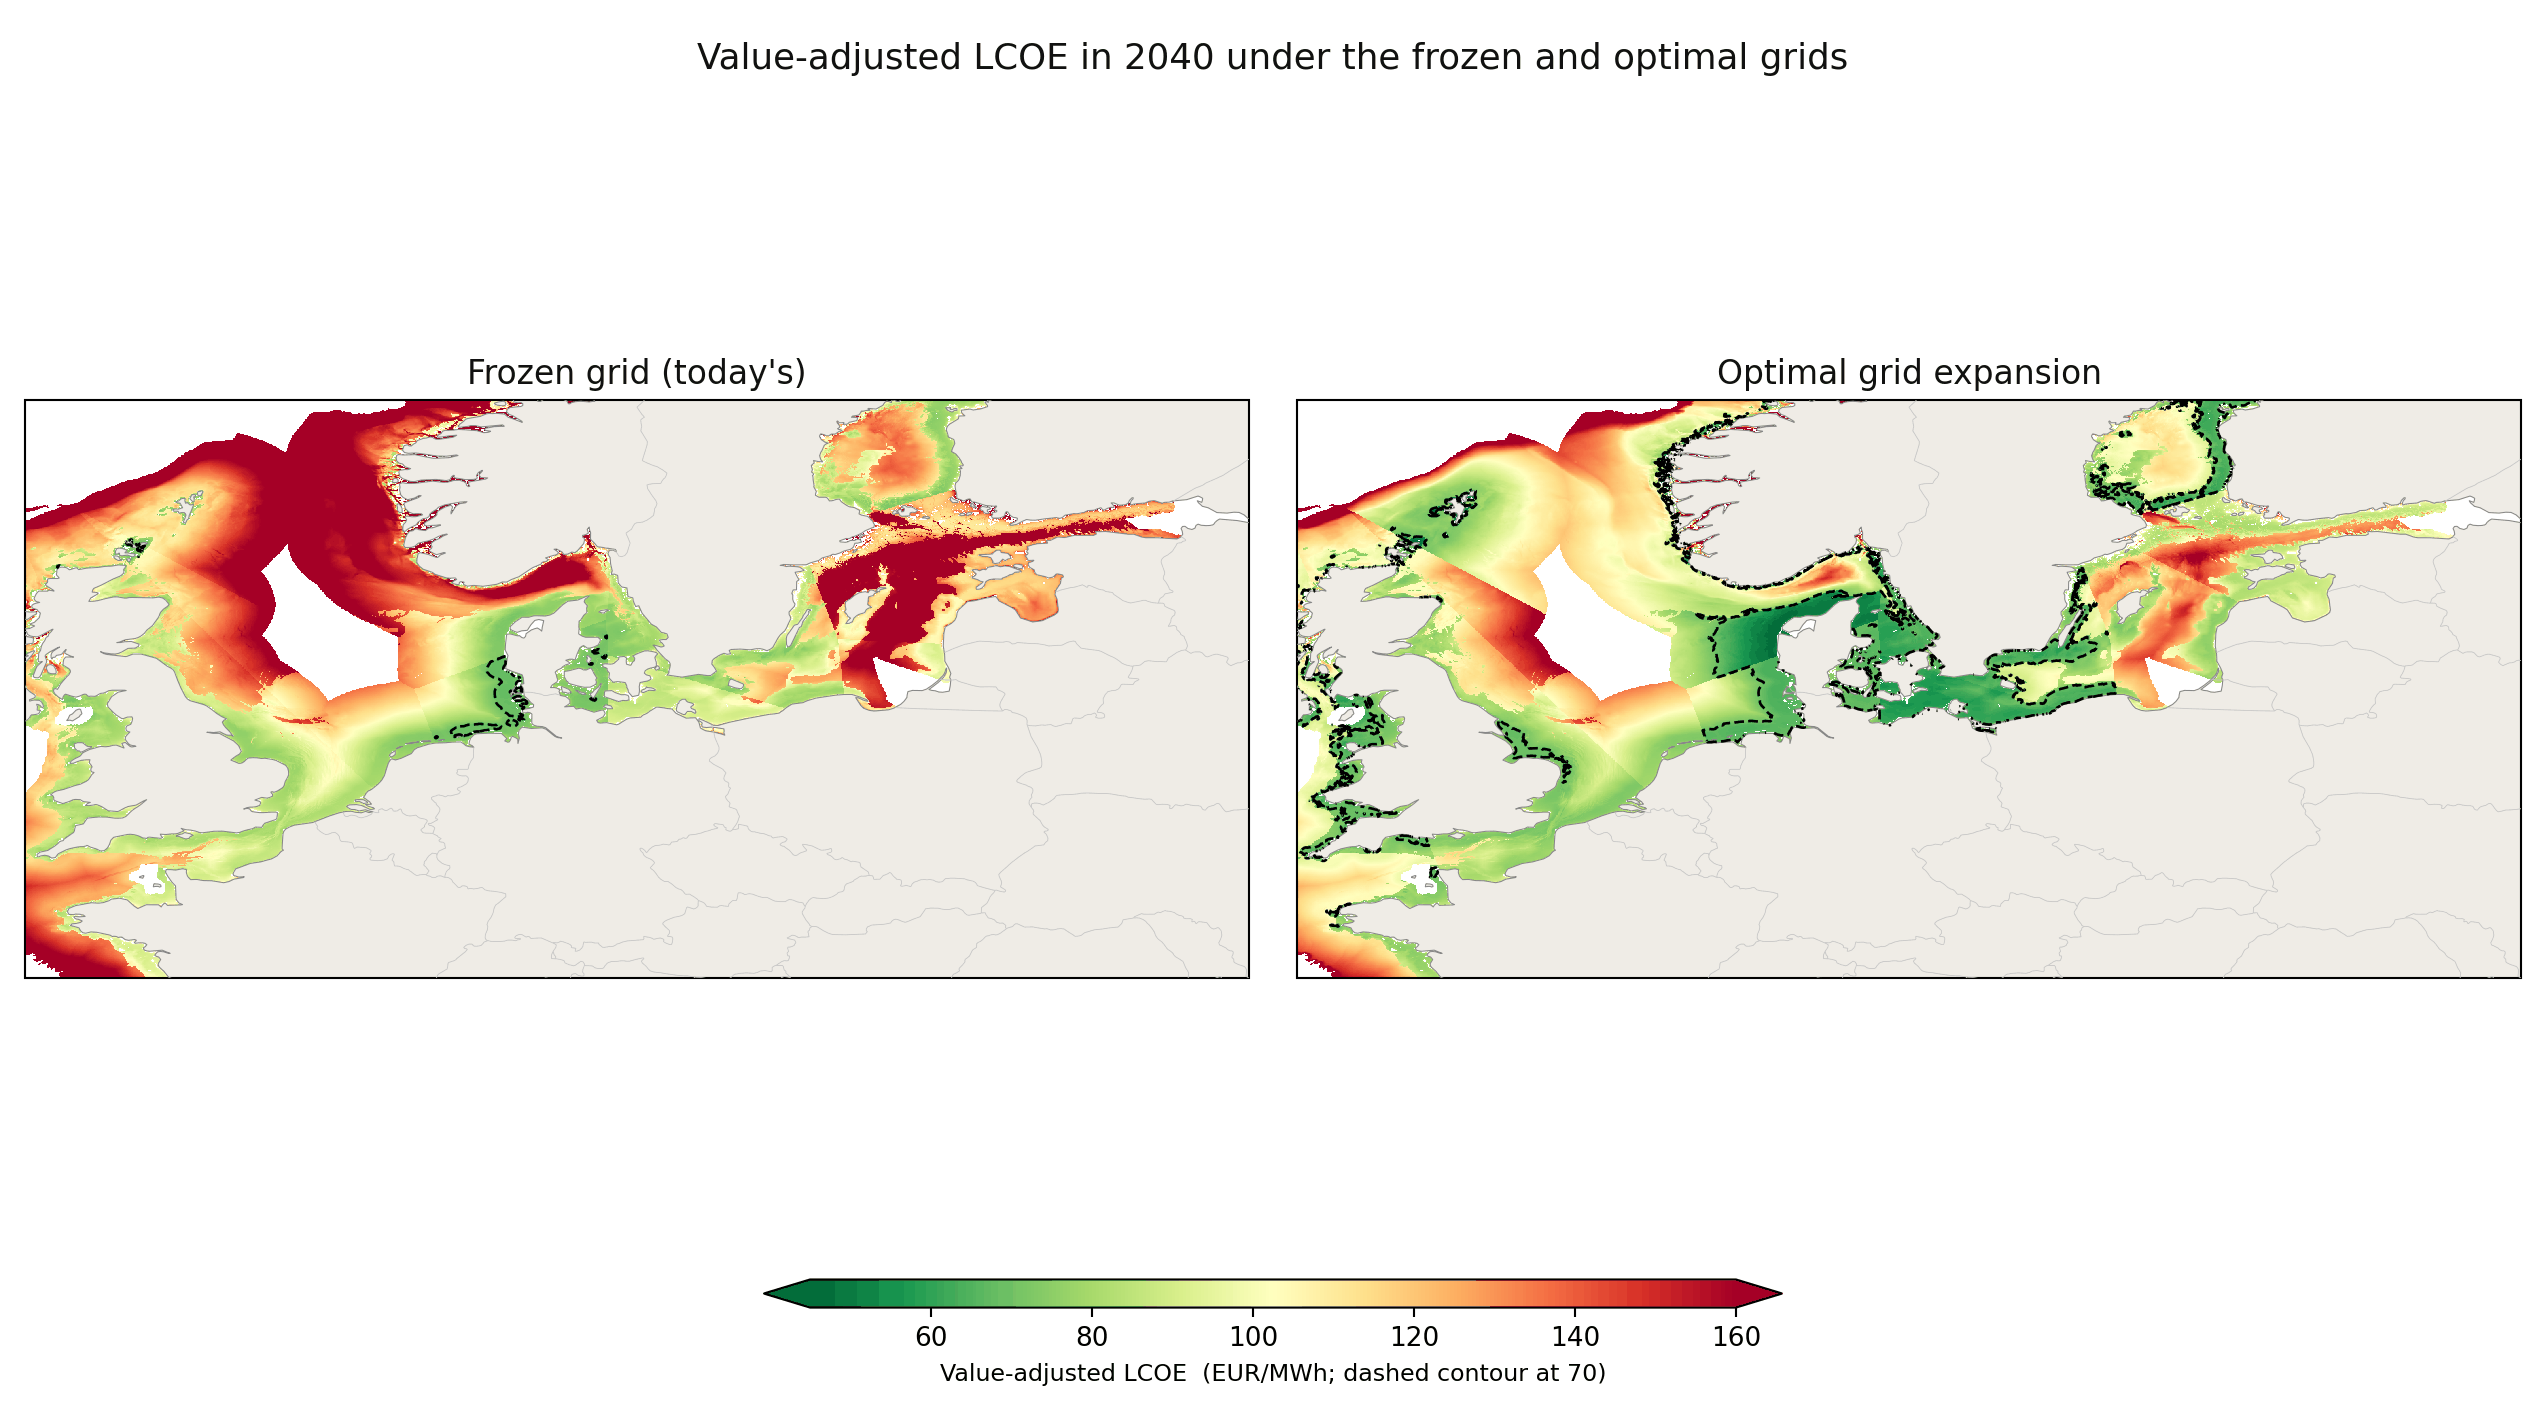
\includegraphics[width=0.96\textwidth]{fig_vlcoe_grid_2040}
    \caption{The 2040 break-even price with the transmission grid held at
    today's capacity (left) and free to expand (right), with offshore cost
    identical in both. The price falls most where the Baltic is enclosed.}
    \label{fig:vlcoe_grid}
\end{figure}

\subsubsection{Effect of capture value on site ranking}\label{sec:site_ranking}

Ten candidate development areas, one in each offshore bidding zone, were ranked
twice in each year: once on levelised cost alone, and once on the break-even
price that includes capture value. Comparing the two orderings shows how much
capture value changes where a developer would build
(Figure~\ref{fig:site_ranking}).

\begin{figure}[!htb]
    \centering
    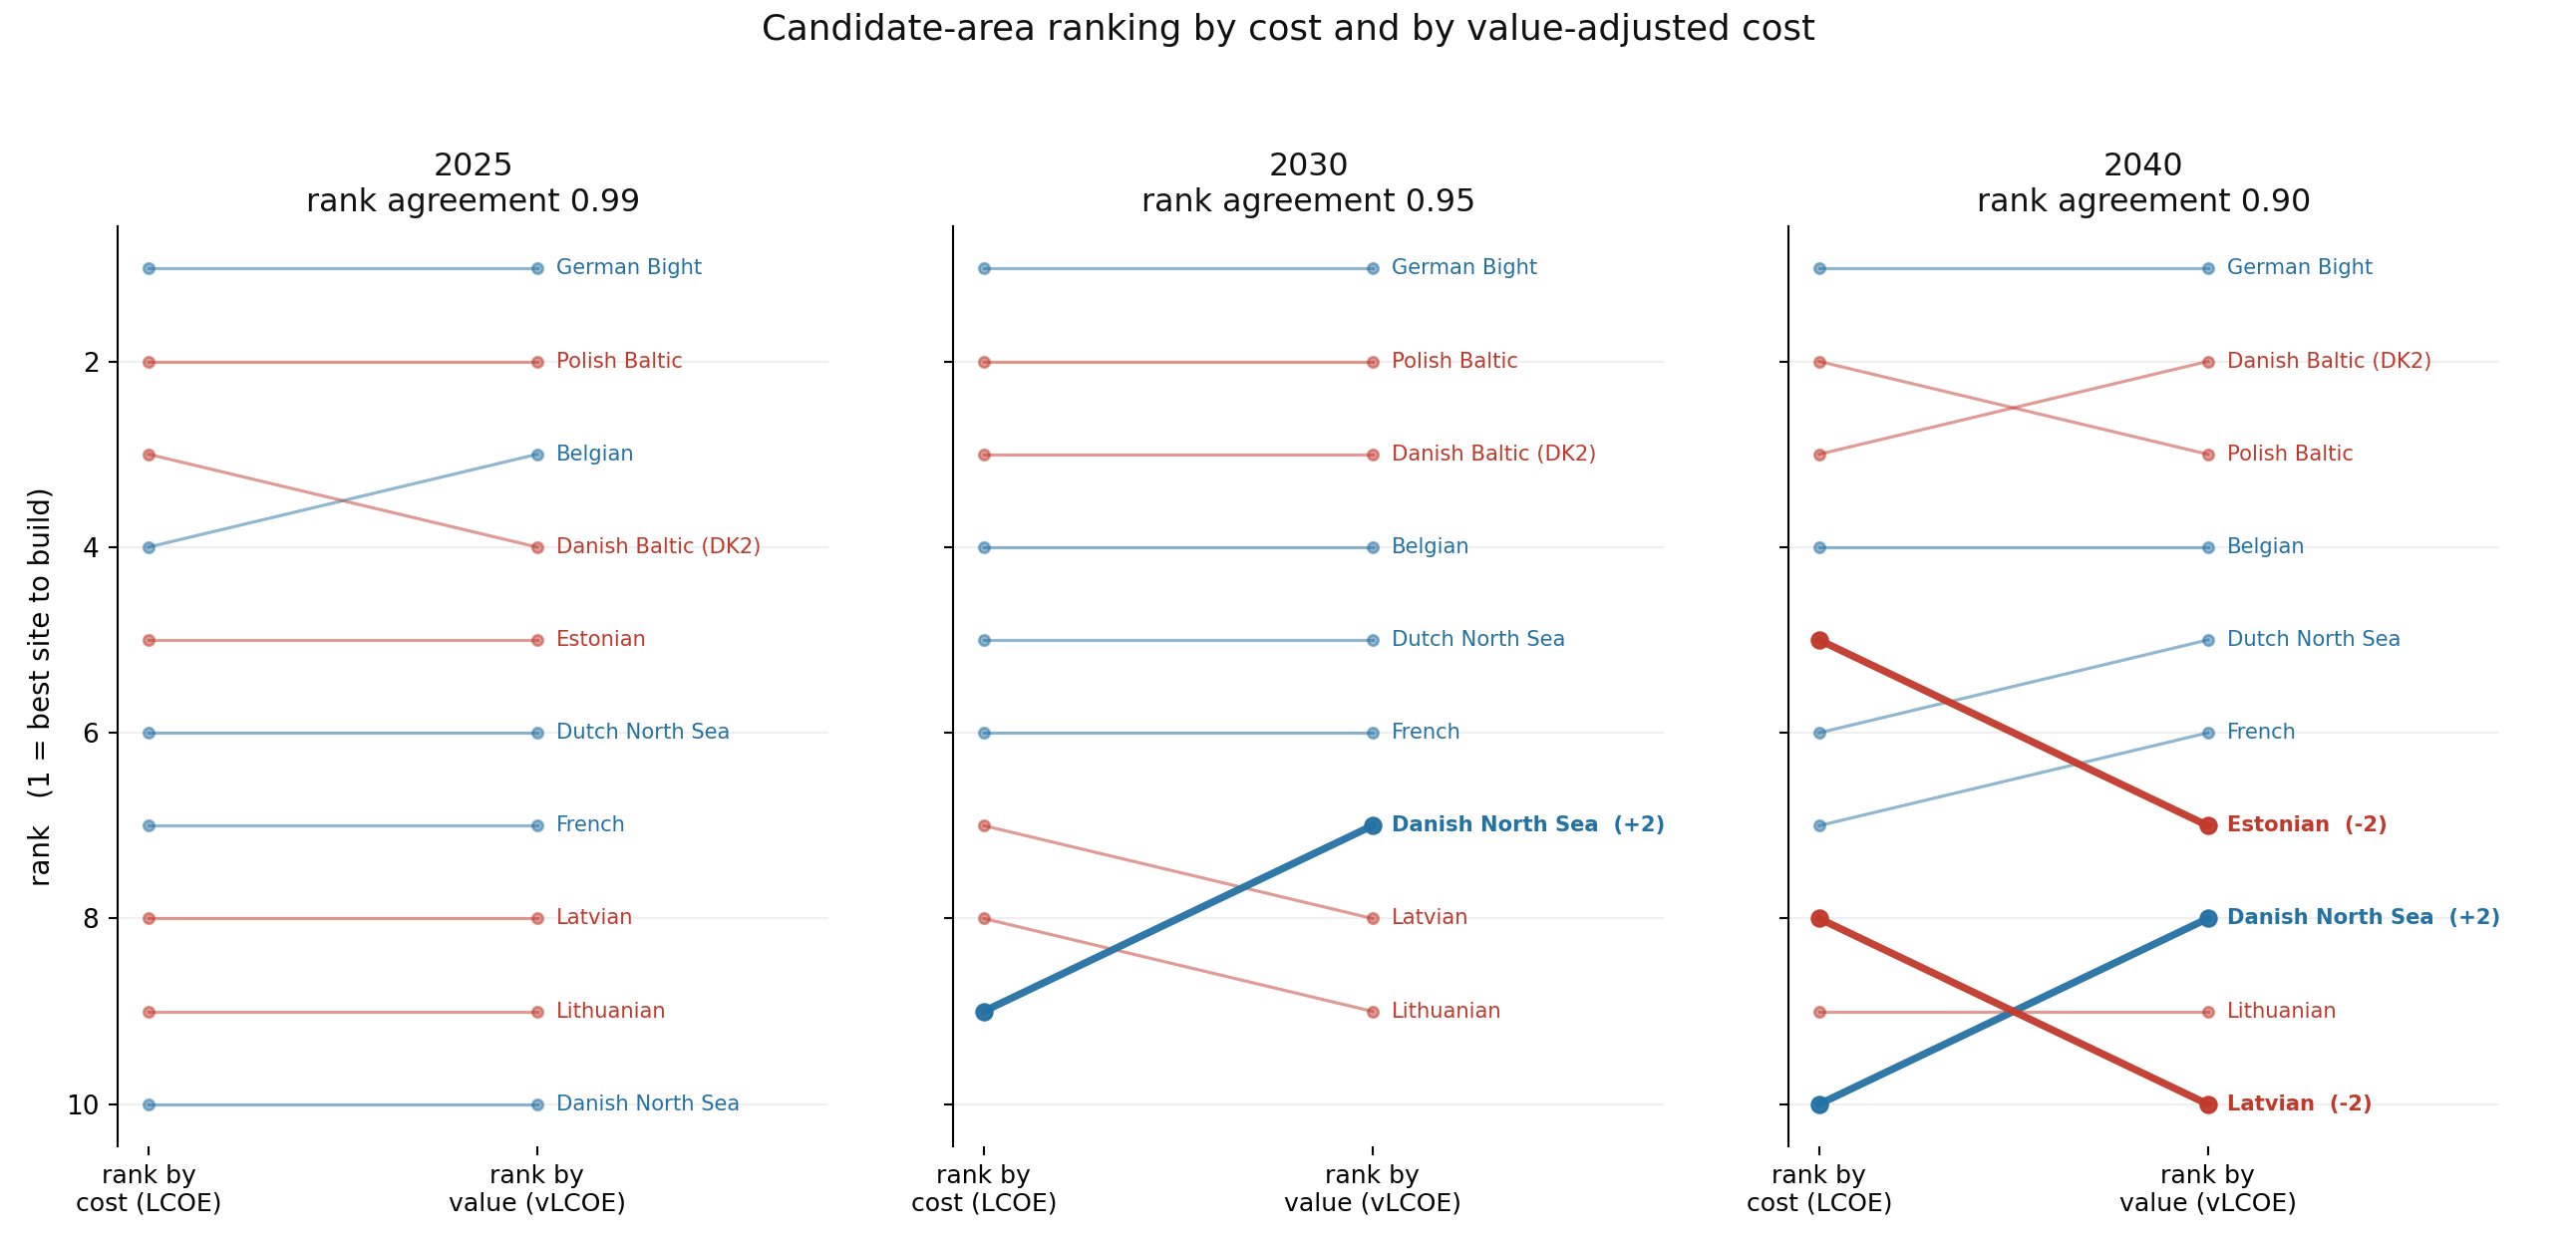
\includegraphics[width=0.94\textwidth]{fig_site_ranking}
    \caption{Candidate development areas ranked on cost alone against the
    break-even price, 2025 to 2040. Areas that hold their position lie on the
    diagonal, and bold lines mark moves of two places or more, in blue for the
    North Sea and red for the Baltic.}
    \label{fig:site_ranking}
\end{figure}

The ranking by levelised cost alone and the ranking by break-even price agree
almost perfectly today and drift apart over time, with a rank correlation of
0.99 in 2025, 0.95 in 2030 and 0.90 by 2040 (Appendix~\ref{app:tables}).
Ranking on cost alone is therefore adequate for a project being built now, and
increasingly misleading for one being built into the 2040s, which is the
period over which offshore wind is financed.

The individual movements identify the misranked areas, and the clearest case
is the cheap eastern Baltic: Estonia has one of the lowest levelised costs on the shelf at 51~\euro/MWh, but
at a capture value of 0.39 its break-even price is 130~\euro/MWh. The Danish
areas rise, because their capture value holds up. The German Bight ranks first
on both measures in every year, having the strongest wind in shallow water close
to shore.

Widening the comparison to 169 candidate locations across both seas gives the
same answer. Whether areas are judged on value for money or on absolute profit,
the German Bight and the shallow western Baltic come first, and the cheap
eastern Baltic scores well on cost and poorly on value
(Appendix~\ref{app:atlas}).

Cost alone remains a defensible basis for the current round of projects,
and a progressively worse one as the buildout advances, with the error
concentrated in the cheap eastern Baltic sites it would promote.

Who bears the resulting loss is a separate question, worked through in
Appendix~\ref{app:portfolio}. Splitting each basin's loss into the part a
support contract absorbs and the part it does not shows that the two basins
differ beneath similar headline numbers: 18.5\,\% of Baltic energy on today's
grid earns nothing at all, while the whole of the North Sea's loss falls outside
what a contract compensates. Building the grid both reduces the loss and changes
who carries it.

% ----------------------------------------------------------------------------

% ============================================================================
% Chapter 5 · Discussion
% ============================================================================

\section{Discussion}\label{sec:discussion}

This chapter answers the three research questions against the evidence of
Chapter 4, sets those answers against the literature and gives the limits of the work and what follows
from them.

\subsection{Answers to the research questions}\label{sec:one_figure}

\textbf{The first question asks how capture value in the enclosed Baltic
compares with the open North Sea today, and how it changes under the committed
buildout to 2030 and 2040.} The two basins are level today: offshore farms in
the under-built Baltic zones capture 0.883 of the average wholesale price
against 0.879 in the North Sea, which is to say that a farm in either basin
received close to 88 per cent of the price a plant generating continuously
would have received over the same period. The fall is modest to 2030 and steep
after it. By 2040, under National Trends, the pathway of the official plan
that tracks existing national policies, the Baltic falls to 0.47 while the
North Sea holds 0.57, so a basin that begins level has lost close to half of
the value it captures today. That outcome depends on the network built
alongside the farms, since with transmission free to expand the Baltic
recovers to 0.66 against the North Sea's 0.64. How much grid is built therefore decides how far the Baltic
falls behind, although even under the most favourable grid tested it still
captures about 0.2 points less than it does today.
Figure~\ref{fig:group_arc} shows the measured record and the projection in one
view.

\begin{figure}[!htb]
    \centering
    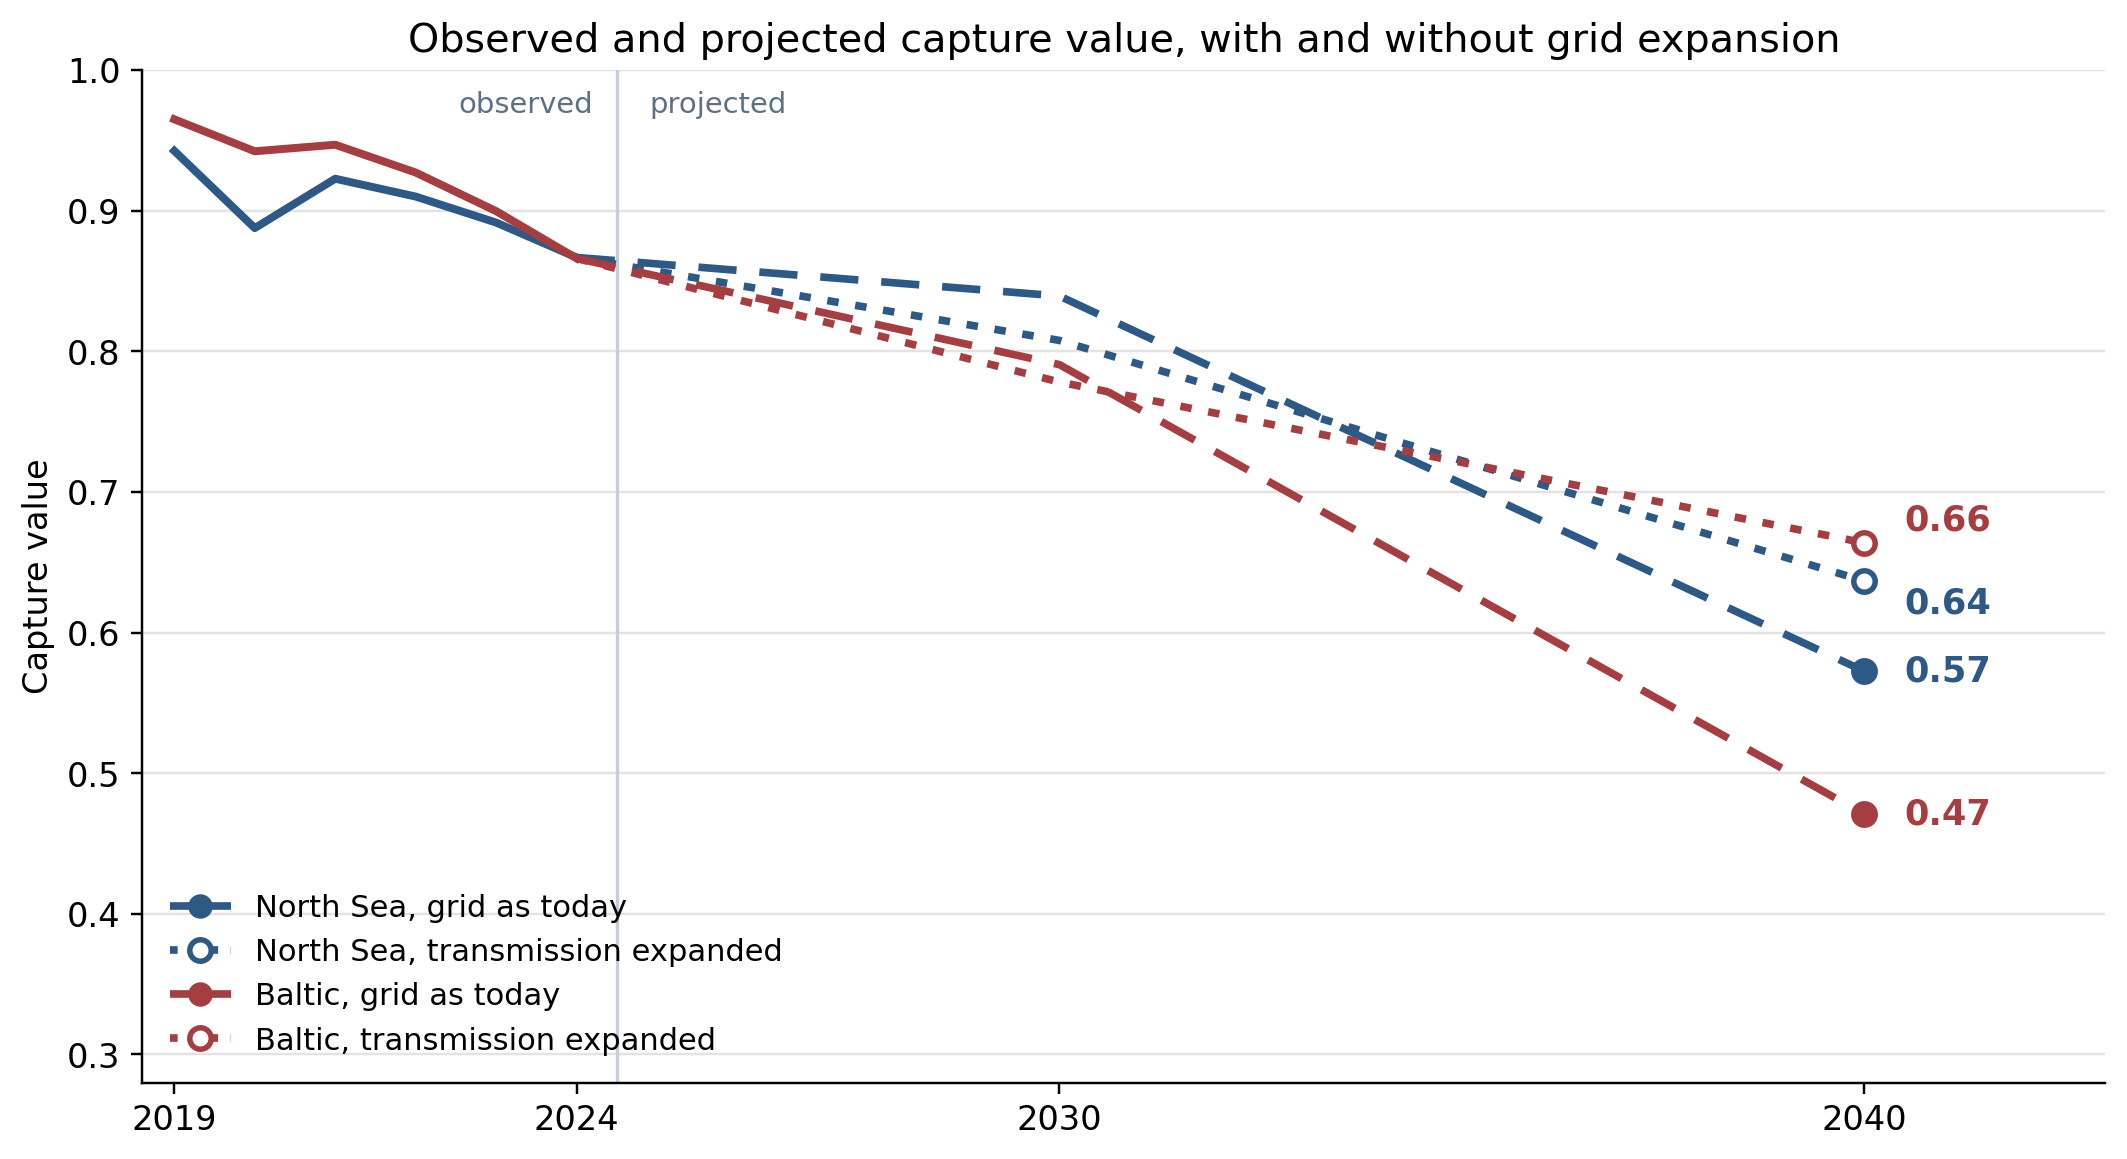
\includegraphics[width=0.95\textwidth]{image-1787753091449.png}
    \caption{Capture value for the North Sea and the Baltic, measured to 2024
    and projected to 2040 under National Trends with the scheduled buildout,
    on today's grid. Solid lines are observed values and dashed lines the
    projection. The Baltic line covers the zones that build out, Poland,
    Estonia, Latvia and Lithuania. The full scenario set and the corrected
    values are in Section~\ref{sec:corrected_projection} and
    Appendix~\ref{app:robustness}.}
    \label{fig:group_arc}
\end{figure}

\textbf{The second question asks which mechanisms set the rate at which capture
value is eroded, whether they differ between an enclosed and an open basin, and
how much of that erosion system design can remove.} Between individual farms the
largest single cause is crowding, meaning how closely a farm's output coincides
with that of the rest of the system, since a farm generating when everything
else generates is selling into hours in which the price has already been driven
down. The same mechanisms operate in both basins and are simply stronger in the
Baltic, where the penalty for generating alongside everything else is twice as
large as in the North Sea.

A substantial part of the resulting loss can be removed by building differently.
Of the 0.42 the Baltic loses under National Trends, 0.19 is congestion that an
expanded grid removes while 0.23 comes from the buildout itself, so nearly half
of the loss follows from the network around the basin. Allowing demand to shift
in time recovers a comparable amount to expanding the grid, 0.28 against 0.19,
which means the two levers available to a system planner are of similar size
(Table~\ref{tab:drivers}).

\begin{table}[!htb]
\centering\small
\caption{The Baltic fall attributed, in the 2040 National Trends scenario
unless stated otherwise. Each component is measured in the section given. The
last two rows are the two design levers, and they add value.}
\label{tab:drivers}
\begin{tabular}{l c l}
\toprule
\textbf{Component} & \textbf{Capture value} & \textbf{Section} \\
\midrule
Total fall, today to 2040 on today's grid & $-0.42$ &
\S\ref{sec:corrected_projection} \\
\quad the buildout itself, which no grid removes & $-0.23$ &
\S\ref{sec:decomposition} \\
\quad congestion, which an expanded grid removes & $-0.19$ &
\S\ref{sec:decomposition} \\
Scarcity pricing inside the stressed scenarios & up to $-0.15$ &
\S\ref{sec:scarcity_results} \\
Winter concentration (winter 0.50, summer 0.83) & seasonal &
\S\ref{sec:seasonality} \\
Recovered by expanding transmission & $+0.19$ & \S\ref{sec:grid_results} \\
Recovered by fully flexible demand & $+0.28$ & \S\ref{sec:sector_results} \\
\bottomrule
\end{tabular}
\end{table}

\textbf{The third question asks whether a model trained on historical
observation can project these futures, whether a system model is required, and
how the two should be combined and validated against each other.} A model
trained on observation cannot project them, and the reason lies in what each
kind of model contains.

The regression model learns a relationship between seven market conditions and
capture value from prices that have already occurred, which is why it reproduces
the recent record more closely than the system model does. The model has
inherited that accuracy from the record, and it holds only while conditions
resemble the ones the model was fitted on. Once the system changes
fundamentally, the association the model learned no longer describes the system
it is being asked about.

The system model contains no fitted relationship at all. It is assembled from
the plants and what it costs to run them, the network and what it can carry, and
demand in every hour, and it re-derives the price in each hour by finding the
cheapest way to meet that demand. Because the mechanism is built in, changing
the fleet changes the answer for the right reason, and the model responds to a
scenario that has never occurred. The price of building the mechanism is that it
must be simplified before it can be solved.

The measurements support this account of the two models, since over the
observed record the two are equally accurate, each missing observed capture value by about 0.04 on average across
144 combinations of zone and month that neither had been fitted on
(Table~\ref{tab:skill}). Beyond that record 90 per cent of their disagreement
at 2040 comes from the regression model no longer responding to the scenario,
while the two continue to agree on how prices are formed. To locate that
boundary, the regression model was refitted on data ending in 2021 and asked
for 2023 and 2024. The two models projected those years equally well, since
most of the targets still lay inside the conditions the regression model had
seen, so the limit is the edge of the observed record rather than the number
of years ahead.

Their construction assigns their roles (Table~\ref{tab:models}). The regression
model, fitted to 2,706 monthly observations from 31 farms, measures the present
and forecasts over horizons short enough that market conditions remain
recognisable. The system model, solved hourly across thirty nodes under official
capacity trajectories, is the only instrument that can price the 2040 fleet, and
it carries the projection with its measured overstatement subtracted.
\subsection{Findings in relation to the literature}\label{sec:disc_literature}

The flexibility offered by hydro was expected to protect the Baltic from a sharp
decline in capture value, and it does not. Hirth finds that systems with a large
hydro fleet hold wind value better than systems built on gas and coal, by about
eighteen percentage points of capture value once wind reaches 30\,\% of supply,
because reservoirs absorb the surplus produced on windy days \cite{Hirth2013}.
The Baltic has that hydro, so on Hirth's reasoning its zones should capture more
of the average price than the North Sea's, whereas the measured record puts the
two level at 0.883 against 0.879 with almost none of the Baltic's offshore
pipeline yet built (Table~\ref{tab:archetype_measured}). The
expectation was built into the design of this thesis, since the archetype table
of Chapter 2 marked the hydro-buffered markets as favourable before the
measurement was made. The explanation is one of scale, since the storage available around the Baltic is small relative to the
surplus a full buildout would produce, and once that storage is full the
remaining power has nowhere to go, because the basin has little capacity to
export it. Hirth's effect operates within a market, and the difficulty in the
Baltic is moving power out of one.

The projection reported falls further than any published for a European
offshore basin. The Baltic's central 0.47 in 2040 sits below the worst North Sea
case Jacquet reports \cite{Jacquet2024}, and it does so at the resolution at
which prices are set, where earlier work reports national averages. The same work
identifies winter as the season in which cannibalisation concentrates, and the
results sharpen that finding, because the two seas are windy at the same
time in winter, so export capacity is least useful in the months when output is
highest, and by 2040 almost the entire annual loss falls in that season, at 0.50
in winter against 0.83 in summer.

Efthymiadou's finding for the United Kingdom, that it is how much
interconnection is actually used, and not the presence of the capacity alone,
that steadies prices \cite{Efthymiadou2025}, is extended here, since relieving the transmission constraint
lifts the most stressed 2040 scenarios by about 0.2 in capture value while
allowing demand to move in time is worth a comparable amount. Those two changes
to the physical system are the largest levers identified anywhere in this work.
Stiewe et al.\ represent the influence of neighbouring markets as a single fixed
coefficient for each zone \cite{Stiewe2025}, which holds that influence constant
over time, whereas in this case the same penalty grows as more capacity is built and can
be separated into the part congestion causes and the part the buildout causes.

Every published benchmark sits above the values projected, whether Hirth's
range of 0.5 to 0.8 at a 30\,\% share \cite{Hirth2013}, Germany's measured 0.76
at 35\,\% \cite{Stiewe2025, Ember2025}, or the roughly 0.6 of Jacquet's worst
North Sea case \cite{Jacquet2024}. Each of those was measured in a more open
market and at a lower level of wind than the Baltic reaches in these scenarios,
so the difference between them reflects where each sits on the same curve. The
panel literature reinforces that reading, having established that the decline
steepens as penetration rises \cite{LopezProl2024, Cevik2022}, which extends the
published trajectories into the range projected.

The two models behaved as the literature predicts in one respect and not in the
other. A model fitted to data is conventionally expected to understate the
spread of the observations, while a model built from physical and cost
relationships is expected to carry a consistent offset \cite{Theil1966}. The
system model behaves as expected, reading consistently too high by 0.041 on
average, but the regression model does not, since it reproduces the spread of
the observations accurately and its error lies almost entirely in which months
it places high and which low. What it has learned, in other words, is how much
cannibalisation there is without learning when it occurs, which is a more
forgiving failure when the task is to measure today's level than when the task
is to rank one month against another.

\subsection{Limitations and future directions}\label{sec:conc_limitations}

The complete register of assumptions is given in Appendix~\ref{app:assumptions}.
The limitations capable of altering a reported value are set out below, each
with the work that would resolve it.

The bias correction is fitted on a single high-penetration zone. DK2 is the only
validation point at an offshore share comparable to the projected Baltic, and
removing it leaves a correction that no longer increases with buildout, so the
correction is reported as a refinement and the values quoted throughout
come from the uncorrected system model (Appendix~\ref{app:robustness}).
Resolving this requires further validation points at high penetration, which
will become available as the Baltic fleet is commissioned.

The system model solves a linear dispatch and does not represent
generating units that must remain online or that bid below their marginal cost.
This is the source of the overstatement in DK2, and replacing the assumed
interconnector ratings with the capacities offered to the market corrects DK1
without correcting DK2. Representing unit commitment and must-run heat
production explicitly would address it directly, at a substantial increase in
computational cost.

The accounting of who bears the loss covers generated energy only and does not
include curtailed volume, which amounts to a third of North Sea wind output on
the 2040 network held at today's capacity. Including curtailed energy, and
solving at intermediate levels of network expansion so that the planned network
is priced alongside the present and the fully expanded cases, would complete
that accounting.

Great Britain and Norway do not pass validation at the spatial resolution used and are excluded from every reported aggregate, although the three British
farms remain in the regression model's training data up to 2020, when British
prices left the ENTSO-E platform. Great Britain is a suitable subject for a
separate application of the same design, since its market record is public and
nothing after 2020 has been used.

Only DK2 and one Swedish farm have operating offshore capacity in the enclosed
Baltic, so the remaining zones are represented by the validated virtual wind
farm, since local measurement does not exist there. The regression model nevertheless
predicts six of the seven enclosed zones to within 0.07 of the observed value
when those zones are withheld from fitting, and metered output from the farms
now under construction would allow this to be tested directly.

The projection holds the correlation between wind patterns and the utilisation
of interconnection fixed at present values, and the fast approximation used for
the wider scenario sweep becomes optimistic at the highest levels of buildout.
For both reasons the values reported come from the direct zone-by-zone solves,
with the present network and the fully expanded network bounding the result.

Two extensions follow from this work. The first is geographic. The design uses
open data, an open resource model and an open system model throughout, so it can
be applied wherever hourly prices and a network representation exist, and
extending it beyond the two basins studied in this work would allow offshore potential
to be assessed on the value of the electricity produced rather than on the wind
resource alone, across a considerably wider set of markets. The second concerns
sector coupling. The sector-coupled solve reported is a single sensitivity,
and it shows that flexible demand recovers as much capture value as network
expansion does, which makes the assumption about future flexibility one of the
largest open questions in the result. Running the complete scenario set in
PyPSA-Eur-Sec, rather than as a bracket applied to one case, would establish how
much of the projected erosion survives once heat, transport and hydrogen demand
are optimised alongside electricity.
% ============================================================================
% Chapter 6 · Conclusion
% Style: no em dashes; synthesise, do not re-argue; answer each RQ directly;
% state each headline number once; limitations and future work relocated here
% from the discussion to avoid duplication.
% ============================================================================

\section{Conclusion}\label{sec:conclusion}

In 2024 the German day-ahead price fell below zero for 459 hours, and this
thesis set out to establish what happens to the value of offshore wind once
hours like these become a sea basin's ordinary operating state. Europe is
committed to the buildout that will produce them: Baltic offshore capacity is
planned to grow from 2.6 to 49.5~GW by 2040, a nineteenfold increase against a
ninefold increase around the North Sea, while support moves away from fixed
payments towards contracts that leave generators exposed to the wholesale
price. What a farm earns therefore depends on the price prevailing in the
hours it generates, and those are the hours its neighbours generate too.

This thesis measured the share of the average wholesale price that offshore
wind actually receives, its capture value, for every bidding zone around the
two seas, and projected it to 2030 and 2040. Over 2023 and 2024 the Baltic
zones that have built little so far captured 0.883 of the average price, level
with the North Sea's 0.879. By 2040, on today's grid, they fall to 0.47 under
National Trends, the pathway of the official plan that tracks existing
national policies, while the North Sea holds 0.57, so close to half of present
value is lost. The ordering of the two basins reverses within fifteen years.

The largest single cause at the level of an individual farm is crowding,
meaning how closely a farm generates at the same time as everything else, and
the penalty for it is twice as steep in the Baltic as in the North Sea. At the
level of the system the fall divides in two. Of the 0.42 the Baltic loses,
0.23 comes from the buildout itself and 0.19 from congestion, and the
congestion part disappears once the grid is expanded: with transmission free
to grow the Baltic recovers to 0.66 against the North Sea's 0.64. Nearly half
the loss, in other words, is a consequence of what gets built around the
farms.

Which of the two models could make that projection had to be established
rather than assumed. Over the years that can be checked against observation
the statistical model and the system model are equally accurate, and their
estimates of capture value agree to within 0.005. Beyond those years ninety
per cent of their disagreement at 2040 is the statistical model ceasing to
respond to the scenario, because it inherits the present instead of
reconstructing it. The statistical model therefore measures the present and
the near term, and the system model, which rebuilds prices from plants, costs
and the network, carries the projection.

The first of this work's four contributions is a systematic comparison of
offshore capture value between the North Sea and the Baltic at the resolution
of the bidding zones in which prices are set, carried from today's measurement
through to the 2040 buildout. The second sets a statistical model and a system
model against observation and against each other on the same measured
quantity, and establishes by measurement the point at which a projection must
pass from one to the other. The third divides the loss of capture value twice,
into the part no network removes and the congestion part an expanded network
does, and into the shares of the loss borne by the farm and by the state under
the contracts that now dominate support. The fourth computes a value-adjusted
cost of energy for each location rather than for each technology, so that a
measured fall in value can be read as the price a specific site must earn.

What the Baltic buildout earns will be decided by the investments delivered
alongside it. Expanding transmission removes most of the congestion loss, and
the income the congested grid already generates, which European law sets aside
for exactly this use, would cover the planned transmission programme several
times over. Allowing demand to move into the windy hours is worth as much
again. The value of Baltic offshore wind is therefore set by decisions that
are still open, and most of that capacity has not yet been built.

% ----------------------------- back matter ---------------------------------
\newpage
\bibliographystyle{unsrt}
\bibliography{references}

\appendix
% ============================================================================
% Appendices. A: farm registry (TODO). B: assumptions register (drafted
% 2026-06-12, post-2024-refit; every value verified against configs, scripts,
% and track READMEs). C: extended tables (TODO). D: reproducibility (short
% draft). E: supplementary figures (TODO). Style: no em dashes.
% ============================================================================

\section{Farm Registry and Data Inventory}\label{app:registry}

The study set is the 31 offshore wind farms of Table~\ref{tab:registry}, sixteen in
the North Sea and fifteen in the Baltic, spanning operational, under-construction,
and planned sites. Each farm's coordinates fix the ERA5 cell its virtual wind farm
samples (Section~\ref{sec:vwf}); capacity and commissioning year are carried for
reference and never enter the capture-value ratio, which is normalised so that rated
capacity cancels. Operational farms, where metered generation exists, are the
validation subset; under-construction and planned sites enter only as price-anchored
panel observations (Section~\ref{sec:fitting}). For recently commissioned farms
the same applies to their pre-commissioning years: Hollandse Kust Zuid came
online in 2023, so its earlier panel rows rest on the validated virtual wind
farm rather than metered output, the method's standard treatment of
not-yet-built capacity. The four German-licensed farms that
stand in Baltic water (zone DE\_LU) are listed under the Baltic by geography but sell into the open German price, so they capture North-Sea-like value.

\begin{table}[!htb]
\centering
\footnotesize
\caption{The 31-farm study registry: market area, location, capacity, commissioning
year, and status. Coordinates are the farm centroid used to select the ERA5 sampling
cell. Sources are developer disclosures, the Crown Estate, and national energy
agencies.}
\label{tab:registry}
\begin{threeparttable}
\begin{tabular}{l l l r r r r l}
\toprule
\textbf{Farm} & \textbf{Country} & \textbf{Zone} & \textbf{Lat} & \textbf{Lon} &
\textbf{MW} & \textbf{Year} & \textbf{Status} \\
\midrule
\multicolumn{8}{l}{\textit{North Sea (16 farms)}} \\
Horns Rev 3              & DK & DK1   & 55.69 & 7.73   & 407   & 2019 & Operational \\
Anholt                   & DK & DK1   & 56.60 & 11.21  & 400   & 2013 & Operational \\
Borssele 1-2             & NL & NL    & 51.70 & 3.02   & 752   & 2020 & Operational \\
Borssele 3-4             & NL & NL    & 51.70 & 2.95   & 731   & 2020 & Operational \\
Hollandse Kust Zuid      & NL & NL    & 52.30 & 4.20   & 1,525 & 2023 & Operational \\
Gemini                   & NL & NL    & 54.04 & 5.97   & 600   & 2017 & Operational \\
Borkum Riffgrund 2       & DE & DE\_LU & 53.97 & 6.55  & 450   & 2019 & Operational \\
Veja Mate                & DE & DE\_LU & 54.31 & 5.86  & 402   & 2017 & Operational \\
Hornsea 1                & GB & GB    & 53.88 & 1.79   & 1,218 & 2019 & Operational \\
Hornsea 2                & GB & GB    & 53.95 & 1.90   & 1,320 & 2022 & Operational \\
C-Power                  & BE & BE    & 51.55 & 2.93   & 325   & 2013 & Operational \\
Norther                  & BE & BE    & 51.50 & 2.95   & 370   & 2019 & Operational \\
Saint-Brieuc             & FR & FR    & 48.82 & $-2.55$ & 496  & 2024 & Operational \\
Dogger Bank A            & GB & GB    & 54.75 & 1.85   & 1,200 & 2025 & Under constr. \\
Princess Elisabeth Zone  & BE & BE    & 51.50 & 2.60   & 3,500 & 2030 & Planned \\
North Sea Energy Island  & DK & DK1   & 56.20 & 7.50   & 3,000 & 2033 & Planned \\
\addlinespace
\multicolumn{8}{l}{\textit{Baltic (15 farms)}} \\
Rodsand 1 (Nysted)       & DK & DK2   & 54.55 & 11.71  & 165   & 2003 & Operational \\
Rodsand 2                & DK & DK2   & 54.55 & 11.80  & 207   & 2010 & Operational \\
Kriegers Flak DK         & DK & DK2   & 54.97 & 12.90  & 605   & 2021 & Operational \\
Wikinger                 & DE & DE\_LU & 54.83 & 14.07 & 350   & 2017 & Operational \\
Arkona                   & DE & DE\_LU & 54.78 & 14.12 & 385   & 2019 & Operational \\
Baltic 2                 & DE & DE\_LU & 54.99 & 13.16 & 288   & 2015 & Operational \\
Baltic Eagle             & DE & DE\_LU & 54.79 & 13.92 & 476   & 2024 & Operational \\
Lillgrund                & SE & SE\_4 & 55.51 & 12.78  & 110   & 2007 & Operational \\
Bornholm Energy Island   & DK & DK2   & 55.10 & 14.60  & 3,000 & 2032 & Planned \\
Saare-Liiv               & EE & EE    & 58.30 & 22.50  & 3,000 & 2035 & Planned\tnote{a} \\
Liivi Bay                & LV & LV    & 57.80 & 23.50  & 1,000 & 2030 & Planned \\
Klaipeda offshore        & LT & LT    & 55.80 & 20.60  & 1,400 & 2030 & Planned \\
Baltic Power             & PL & PL    & 55.00 & 17.40  & 1,140 & 2026 & Under constr. \\
Baltyk II / III          & PL & PL    & 55.05 & 17.20  & 1,440 & 2027 & Planned \\
FEW Baltic II / Olhava   & FI & FI    & 64.80 & 24.50  & 1,280 & 2030 & Planned \\
\bottomrule
\end{tabular}
\begin{tablenotes}\footnotesize
\item[a] Saare-Liiv falls on a coastal ERA5 cell and is flagged accordingly.
\item Data coverage: Dutch renewable generation is rescaled to physical capacity
factors (documented ENTSO-E under-reporting); British day-ahead prices end with
Brexit, so the three British farms contribute panel data only through 2020.
\end{tablenotes}
\end{threeparttable}
\end{table}

\section{Assumptions Register}\label{app:assumptions}

Every modelling choice that shapes a number in this thesis is listed here
with its value, its source, and where its influence is tested or bounded.
Items marked (L) reappear in the consolidated limitations of Chapter 5.

\subsection*{B.1 Shared data and definitions}

\begin{enumerate}
    \item \textbf{One capture-value definition.} Generation-weighted price
    over time-mean zone price, on common hours only; zone price is the
    unweighted mean over the zone's network nodes; Denmark splits at
    11$^{\circ}$E into DK1/DK2. Used identically by every component
    (Section~\ref{sec:currency}).
    \item \textbf{Basin membership is geographic.} A farm belongs to the sea
    its foundations stand in; DK2 and SE4 are Baltic-facing although their
    markets sit in the Nordic synchronous area
    (Section~\ref{sec:farm_data}). Corroborated by weather-only clustering
    (Section~\ref{sec:weather_agrees}).
    \item \textbf{ENTSO-E Transparency is the single market-data source}
    (2017 to 2024): prices for 22 zones, load, generation by type, flows,
    capacities. Dutch renewable generation is rescaled to physical capacity
    factors (documented under-reporting); British day-ahead prices end with
    Brexit, so GB farms contribute no farm-months after 2020. (L)
    \item \textbf{ERA5 is the weather truth} (regression: nearest
    0.25$^{\circ}$ cell via Open-Meteo; system model: 0.3$^{\circ}$ yearly
    cutouts via atlite). Its offshore wind-speed bias is not corrected
    explicitly; the Hayes power-curve shift absorbs it, and the end result
    is validated against metered generation (median hourly correlation
    0.88, monthly 0.95, fifteen zone-years).
    \item \textbf{TYNDP 2024 is the scenario authority} for capacities,
    demand, and fuel and carbon prices. The parse covers renewables only;
    the corrections of Table~\ref{tab:corrections} repair the documented
    consequences. (L)
\end{enumerate}

\subsection*{B.2 The system model}

\begin{enumerate}\setcounter{enumi}{5}
    \item \textbf{Scope.} Fourteen countries, 30 clusters with focus
    weights on offshore-heavy markets; Sweden and Norway remain coarse
    (three clusters), so SE is reported with an all-Sweden caveat and NO is
    excluded from headline aggregates alongside GB. (L)
    \item \textbf{Resolution.} Full hourly year (8,760 snapshots; the
    framework drops the 2024 leap day by convention).
    \item \textbf{Frozen transmission} (\texttt{transmission\_limit: v1.0}):
    line and link capacities fixed at today's volume, the conservative
    bound; the optimistic bound is computed explicitly (optimal expansion
    moves clean 2040 scenarios $+0.04$ to $+0.06$, stressed ones $+0.18$ to
    $+0.19$).
    \item \textbf{Year-correct fleets.} Conventional plants filtered by
    commissioning and retirement dates; renewable capacities topped up to
    the run year's national statistics (IRENASTAT via powerplantmatching).
    \item \textbf{Fuel-price overrides} (annual means): 2023 gas
    41.0~\euro/MWh$_{th}$, coal 16.0, lignite 5.5, oil 75.0; 2024 gas 34.7,
    coal 14.0, lignite 5.5, oil 74.0; 2019 uses the 2020 technology-cost
    defaults. Sources: TTF and EUA from the project's monthly series, coal
    from ARA annual means, oil from Brent.
    \item \textbf{Carbon prices}: 25 / 84 / 67~\euro/tCO$_2$ for 2019 /
    2023 / 2024 (EUA annual means), applied through emission pricing.
    \item \textbf{Perfect competition, perfect foresight, linear
    dispatch.} No unit commitment, start-up costs, minimum loads, must-run
    district-heating CHP, or strategic bidding. Consequence: shadow prices
    are too flat in windy hours in small congested zones. This is not left
    as an assumption: it is measured (DK2 bias $+0.143$ in 2023, $+0.141$
    in 2024), explained by the hybrid decomposition, and corrected with
    propagated uncertainty (Section~\ref{sec:bias_method}). (L)
    \item \textbf{Interconnectors are fully available every hour} (no TSO
    de-rating or reservations). Same direction and same treatment as the
    previous item: absorbed into the measured, corrected bias. (L)
    \item \textbf{Scarcity ladder} (correction F): demand response sized at
    5\,\% of each node's peak load offered at 400~\euro/MWh; unserved
    energy at the 4,000~\euro/MWh day-ahead cap; residual unserved energy
    below 0.05\,\% of demand, reported per scenario
    (Section~\ref{sec:scarcity_method}).
    \item \textbf{Scenario corrections A to F} as enumerated in
    Table~\ref{tab:corrections}, including the Danish offshore split
    (65/35 in 2030 to 60/40 by 2040), offshore caps (DK 50, FI 25, SE 35~GW), and
    Poland's announced 3.9~GW of nuclear by 2040.
    \item \textbf{Demand trajectories}: scenario demand is rebased from
    crisis-2023 to 2019 before TYNDP growth; the two countries missing from the scenario tables receive documented growth
fallbacks. All scenario
    horizons are solved on 2023 weather and hourly load shapes, so the only thing that changes across scenarios is the buildout. (L)
    \item \textbf{Hydrogen floor} (correction D): a parametric stand-in
    for sector coupling, with per-country electrolysers, fixed hydrogen
    demand, and a priced import backstop near 35 to 42~\euro/MWh; halving and
    raising its demand by 50\,\% moves the 2040 Baltic capture value by at most
    0.013, and by under 0.01 in the clean DE and GA scenarios
    (Appendix~\ref{app:robustness}). (L)
    \item \textbf{Solver parity.} Gurobi barrier without crossover,
    identical tolerances, for every baseline and every scenario, because
    the bias correction is fitted on interior-point duals and must be
    applied to prices formed the same way.
    \item \textbf{Bias correction.} Linear in the model's own offshore
    penetration; fourteen of fifteen validation points (Netherlands 2019
    excluded as low-confidence observation); clamped at penetration 0.50;
    corrected values floored at zero. The penetration slope is anchored on DK2,
    the only validation zone above 31\,\% penetration: leave-one-zone-out
    collapses it from 0.233 to 0.045 with an interval crossing zero
    (Appendix~\ref{app:robustness}), so the correction is reported as a refinement of the uncorrected system model, which remains the
    source of the result. (L)
    \item \textbf{Gas-price grid}: 15 to 120~\euro/MWh$_{th}$ across three
    buildouts; exposure slopes computed over every offshore zone, with
    basin aggregates excluding GB and NO.
    \item \textbf{Sector-coupled variant}: PyPSA-Eur's sector
    configuration at twelve-hour resolution, thirty clusters, 2019 weather,
    overnight 2040, frozen grid, with heating, hydrogen, storage and
    electric transport co-optimised; country totals pinned to the TYNDP
    2040 fleet (Belgium capped at its 4.9~GW sea-space potential); the
    electricity-only control is identical in every setting. The weather
    cutout spans 47$^{\circ}$N northward, truncating southern France
    identically in both arms. (L)
    \item \textbf{Surrogate emulator}: eight inputs; fifty Latin-hypercube
    training solves at three-hour resolution (full-hourly equivalence
    checked: mean absolute capture-value difference 0.024, up to 0.147
    only at the extreme 139-GW corner); validation by held-out whole
    scenarios; the Baltic correction parsed from the canonical fit. (L)
\end{enumerate}

\subsection*{B.3 The regression model}

\begin{enumerate}\setcounter{enumi}{21}
    \item \textbf{Virtual wind farm}: logarithmic extrapolation from the
    10~m and 100~m ERA5 levels to the 150~m hub height of the IEA 15~MW
    reference turbine \cite{Gaertner2020}, whose power curve enters as a
    hand-keyed table of the published values interpolated on a
    0.25~m\,s$^{-1}$ grid (cut-in 3, rated 10.59, cut-out 25~m\,s$^{-1}$);
    Hayes adjustments $\sigma = 1.17$~m\,s$^{-1}$ and
    $w_0 = 0.71$~m\,s$^{-1}$ (calibrated on 57 metered European farms),
    applied as a Gaussian convolution of the curve followed by a rightward
    shift; output hard-zeroed outside the 3 to 25~m\,s$^{-1}$ operating
    envelope after smoothing, since the convolution otherwise leaks output
    into storm and calm hours. The archived eight-year panel predates this
    re-zero; hours outside the envelope are rare enough to bound its effect
    below half a percent of capture value; the released code applies the re-zero.
    Farms closer than one reanalysis cell share identical output, so
    near-neighbour pairs are excluded from synchronicity comparisons.
    \item \textbf{Monthly capture value} requires at least 500 overlapping
    farm-price hours; capacity factors are normalised, so rated capacity
    cancels in the ratio.
    \item \textbf{Training set}: the bidding-zone market panel, every site
    with observed prices over 2017 to 2024 (all 2,706 zone-months across 31
    sites). The operational farms are the validation subset, the only sites
    where generation can be checked against metered output. (L: metered
    offshore exists only in DK2 and SE4, so the enclosed-Baltic price-only
    zones are anchored on observed prices and a validated wind profile, since no local
    metered generation exists.)
    \item \textbf{Market-area resolution}: features computed at bidding-zone
    level where zone-resolved series exist (DK1, DK2, SE4), country level
    elsewhere, recorded per row. (L)
    \item \textbf{Flexibility index numerator}: openly reported pumped
    hydro plus battery capacity where ENTSO-E reports it, a documented
    substitution for the predecessor's proprietary battery and
    demand-response data. (L)
    \item \textbf{Interconnection index}: realised utilisation, the mean
    absolute cross-border flow over each external border's capacity (proxied
    by its yearly maximum flow), summed across borders. The predecessors'
    neighbour-synchronicity discount is dropped on evidence
    (Section~\ref{sec:features}); static within each year, blind to
    hour-by-hour congestion. (L)
    \item \textbf{Fuel features}: monthly TTF gas and EU ETS carbon
    averages.
    \item \textbf{Collinearity}: variance inflation factors on the 2,706-row
    panel peak at 2.16 (carbon), far below the conventional alarm level of
    five; feature 7 sits at 1.21.
    \item \textbf{No hyperparameter search}; fixed settings for all five
    algorithm families: gradient boosting with 400 trees of depth 4 at
    learning rate 0.05, random forest with 300 trees of depth 8, and
    support-vector, polynomial and linear regression at library defaults
    (library versions in Appendix~\ref{app:repro}); the untuned predecessor
    result is the comparator.
    \item \textbf{2022 retained} in training; an ex-2022 variant is
    reported alongside, mirroring the predecessor's crisis treatment.
    \item \textbf{Projection feature choices}: pattern correlations held
    at the site's recent monthly shape; penetration scaled by TYNDP
    renewable growth over demand growth, anchored on the observed present;
    interconnection held at its recent value (no future border capacities exist in the scenario tables, a mildly
optimistic simplification, with a
    conservative-bound sensitivity that lets utilisation decline as
    renewables grow); flexibility grows with the scenario battery fleet. All
    guarded by the strict all-features range check, the joint convex-hull
    support test, and the carbon-clamp sensitivity. (L)
\end{enumerate}

\subsection*{B.4 The comparison with observation}

\begin{enumerate}\setcounter{enumi}{32}
    \item \textbf{Independence of the three-way comparison's columns}: the regression
    column is out-of-fold (the model never trained on the zone's farms);
    the system column uses no market price data; observation arbitrates.
    \item \textbf{Hybrid decomposition}: model generation priced at
    observed prices isolates whether an error lives in the wind or in the
    price structure.
    \item \textbf{Aggregation difference}: the regression's zone capture
    value is a simple mean over farm-months while the system model's
    is energy-weighted; a small, documented difference.
    \item \textbf{The DK2-analogue premise}: the system model's bias
    transfers along the penetration axis from validated zones to projected
    ones. This is tested directly: the bias replicates across 2023 and 2024,
    the fit's slope interval excludes zero, and no single zone-year moves
    the leave-one-out range.
\end{enumerate}

\subsection*{B.5 The analytical equation in full}

Because an additive split cannot express the shape of the mechanism,
Jacquet's analytical equation is refit as well \cite{Jacquet2024}. It is not a
black box, nor an arbitrary curve: it is a parametric form assembled, term by term,
from the cannibalisation mechanism of Section~\ref{sec:value_problem}. A farm
that sold at random hours would earn the average price, a capture value of one;
cannibalisation is what subtracts from that one. The equation writes that
subtraction as two physical channels, a cannibalisation term and a fuel-price
distortion term, so that every constant in it is a named lever on a specific
channel rather than a free coefficient fit for its own sake:
%
\begin{equation}
    \mathrm{CV} \;=\; 1
    \;-\; B\,\frac{M_{\mathrm{WF}}}{M_{\mathrm{BZN}}}\,S
    \;-\; C\,M_{\mathrm{WF}}\,
    \bigl(0.202\,p_{\mathrm{CO_2}} + p_{\mathrm{gas}}\bigr)^{\gamma}.
\end{equation}
%
where $S$ is the renewable market share and $p_{\mathrm{gas}}$,
$p_{\mathrm{CO_2}}$ the monthly fuel and carbon prices, folded together by the
0.202~tCO$_2$/MWh emission intensity of gas. The first term is cannibalisation:
the wind-pattern penalty $M_{\mathrm{WF}} = \mathrm{sign}(\rho_{\mathrm{VRE}} -
\rho_{\mathrm{load}})\,|\rho_{\mathrm{VRE}} - \rho_{\mathrm{load}}|^{\alpha}$
grows when a farm tracks the system's renewables more than its demand. It is
scaled by penetration $S$ and divided by the buffering term
$M_{\mathrm{BZN}} = (I_{\mathrm{int}} + I_{\mathrm{flex}})^{\delta}$, in which
interconnection and flexibility absorb it. The second term is fuel-price
distortion.

The constants carry the mechanism. The pattern-penalty exponent $\alpha$ sets how
sharply the penalty escalates as a farm's wind aligns with the system's. The
\textbf{cannibalisation scale} $B$ is its overall strength: it multiplies the whole
crowding-times-penetration term, so a larger $B$ means a given amount of crowding
and penetration erodes more value. The \textbf{buffering exponent} $\delta$ governs how strongly interconnection and flexibility reduce that erosion: the penalty is
divided by $(I_{\mathrm{int}} + I_{\mathrm{flex}})^{\delta}$, so a larger $\delta$
makes interconnection and flexibility more protective per unit of capacity. $C$
scales the fuel-price distortion term and $\gamma$ sets its curvature. They are fit
by bounded least squares, separately for the pooled data, the North Sea, and the
Baltic, with a 200-resample farm-block bootstrap for intervals. Because the
constants trade off inside shared terms, no single one is read in isolation; the
basins are compared by the quantity they jointly produce, the implied slope of
capture value against penetration, at common reference conditions.

\subsection*{B.6 The spatial cost model in full}

Offshore capital cost rises with both: deeper water
demands heavier foundations, and farther sites demand longer export cables.
Writing $c_0$ for the turbine-and-array base, $\phi(d)$ for the foundation, and a
linear export term beyond a near-shore allowance $\ell_0$,
%
\begin{equation}
  \mathrm{CAPEX}(d,\ell) \;=\; c_0 \;+\; \phi(d) \;+\; \gamma\,\max(\ell-\ell_0,\,0),
  \qquad
  \phi(d) =
  \begin{cases}
    a_{f}\,\max(d-d_0,0), & d \le d_1,\\[2pt]
    a_{f}(d_1-d_0) + c_{\mathrm{fl}} + a_{\mathrm{fl}}(d-d_1), & d > d_1,
  \end{cases}
  \label{eq:costmodel}
\end{equation}
%
with $c_0 = 1.85$~M\euro/MW, $d_0 = 25$~m, $d_1 = 60$~m, fixed-bottom slope
$a_{f} = 12$~k\euro/MW/m, a floating premium $c_{\mathrm{fl}} = 1.0$~M\euro/MW
appearing past $d_1$, floating slope $a_{\mathrm{fl}} = 6$~k\euro/MW/m, export term
$\gamma = 10$~k\euro/MW/km, and $\ell_0 = 25$~km. The piecewise jump at $d_1$ is
the transition from fixed-bottom to floating foundations. Levels are anchored to
the offshore cost database that ships with PyPSA-Eur and to IRENA's 2024 cost
review \cite{Horsch2018, IRENA2025Costs}. Capital is annualised at a capital
recovery factor $\mathrm{CRF} = w(1+w)^n/[(1+w)^n-1]$ with a weighted-average cost
of capital $w = 7\%$ over an economic life $n$ of 27 to 30 years, technology
learning enters through a factor $\lambda(y)$ normalised to unity in 2025 and
falling on the database's offshore trajectory (capital cost about 2505 to
1916~\euro/kW over 2020 to 2050), and fixed operations cost is
$f_{\mathrm{OM}}(\ell) = 75 + 0.25\,\ell$~k\euro/MW/yr.

\section{Extended Results and Per-Zone Projections}\label{app:tables}

The headline projection of Section~\ref{sec:projection_results} reports the
Baltic at basin-mean resolution. Because the thesis rests on within-basin
spread, Figure~\ref{fig:perzone} resolves it: the Baltic zones that
build out (Poland, Estonia, Latvia, Lithuania, with Finland shown but set
aside as before, since its decline comes from the price collapse that followed the Olkiluoto-3
nuclear startup, and does not reflect wind cannibalisation), each with its modelled capture-value history and its
bias-corrected 2030 and 2040 projection, the vertical bars showing the spread
across scenarios. The history is modelled, since metered revenue does not exist for these
zones: it weights each zone's
observed prices by the virtual-farm output, since these zones have little or no
operating offshore, and most rest on a single planned-farm proxy (Poland on
two). The regression model returns a constant at these horizons, so the projections
are system-model projections, corrected per zone on the fit of
Section~\ref{sec:bias_method}. The zones diverge sharply by 2040, from
Lithuania near 0.40 to Estonia near 0.20, a range the basin mean conceals
and the reason a developer cannot read a single Baltic number off the
headline.

\begin{figure}[!htb]
    \centering
    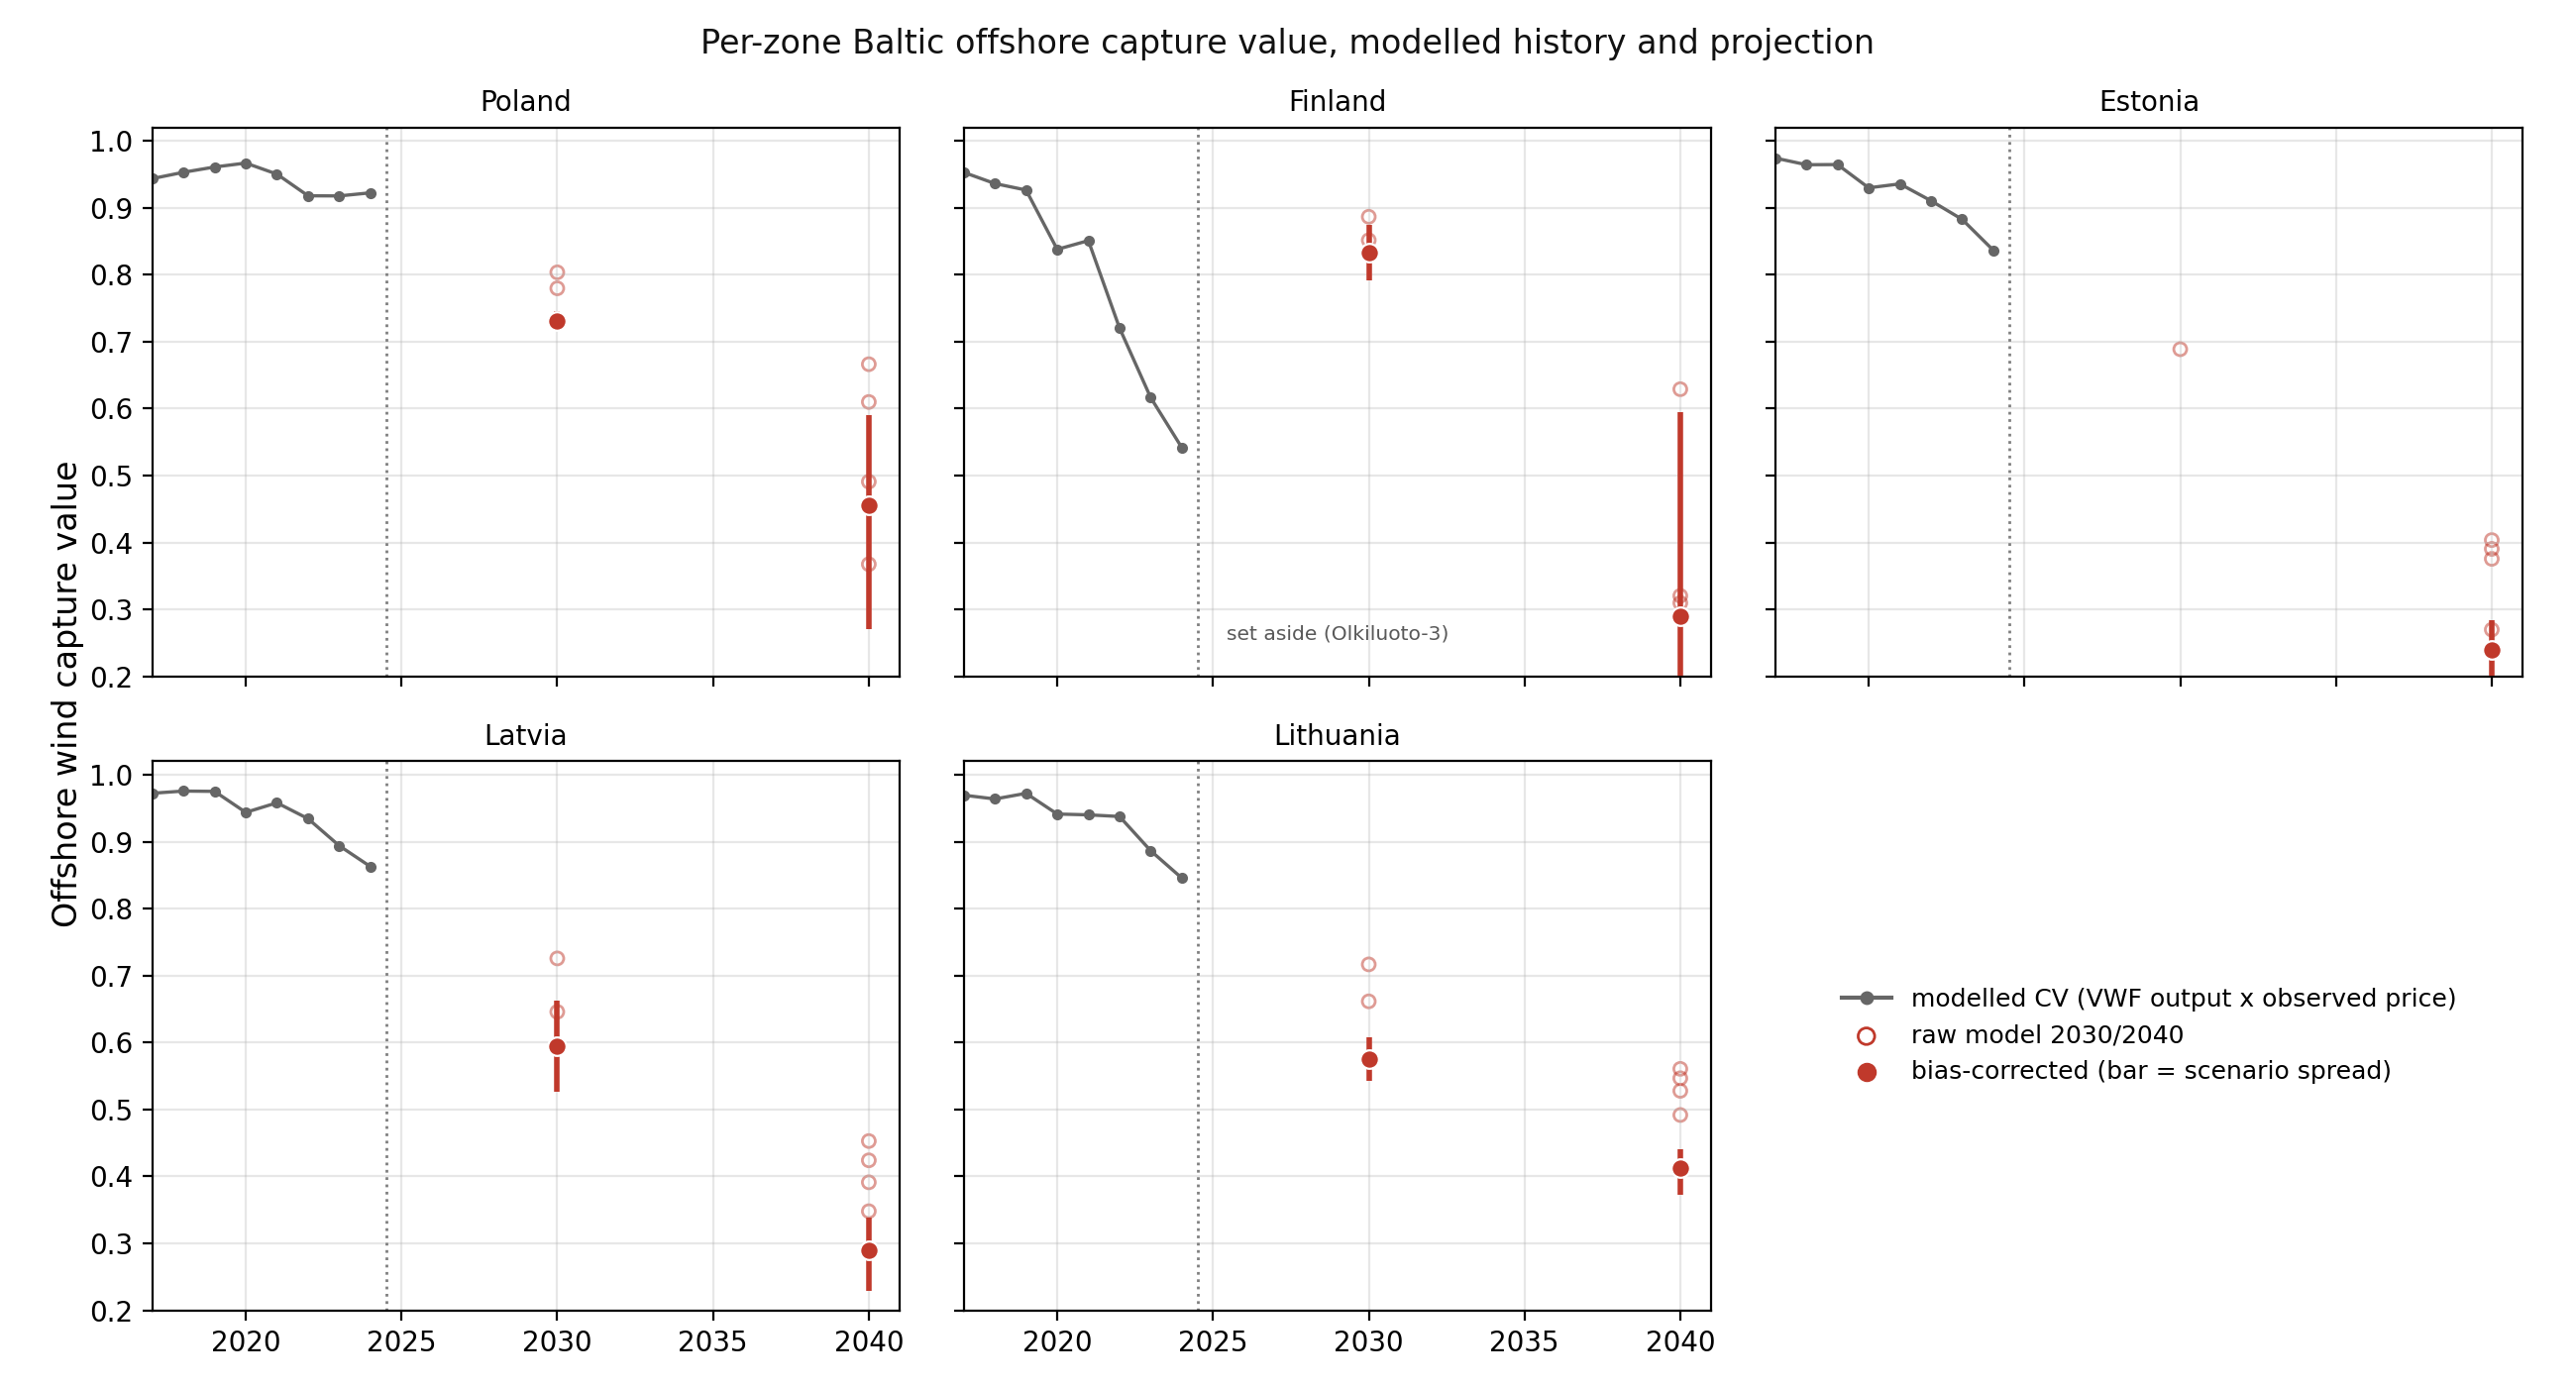
\includegraphics[width=0.98\textwidth]{fig_perzone_projection}
    \caption{Per-zone Baltic offshore capture value, modelled history (2017 to
    2024, grey; virtual-farm output weighted by observed zone prices, as no metered revenue
    exists) to bias-corrected projection (red), for the zones that build out
    (Finland shown but set aside, nuclear-driven). Open markers are the raw model;
    filled markers the bias-corrected central value; vertical bars the spread
    across scenarios at each horizon. The regression model stops responding at these horizons; these are
    system-model projections.}
    \label{fig:perzone}
\end{figure}

\subsection*{C.1 Full algorithm and validation-scheme comparison (regression model)}

Table~\ref{tab:regression_full} extends the headline metrics of
Table~\ref{tab:regression_metrics} to all five algorithm families under every
validation scheme. Gradient boosting leads on every genuine generalisation
test, and the polynomial's large negative out-of-fold scores show how violently a
closed form extrapolates, the instability that makes the tree the operational
model and the analytical equation only an interpretable backup.

\begin{table}[!htb]
\centering\small
\caption{Out-of-fold $R^2$ of all five algorithm families under every validation
scheme, at bidding-zone feature resolution. A dash marks schemes run only for
the headline model. These metrics are independent of the system-model re-solve.}
\label{tab:regression_full}
\begin{tabular}{l r r r r r}
\toprule
\textbf{Validation scheme} & \textbf{XGBoost} & \textbf{Random forest} & \textbf{SVR} &
\textbf{Poly(2)} & \textbf{Linear} \\
\midrule
Random K-fold (Jacquet scheme)    & 0.752 & 0.682 & 0.583 & 0.437 & 0.330 \\
Leave-farm-out (headline)           & \textbf{0.686} & 0.636 & 0.497 & $-19.9$ & 0.270 \\
Leave-farm-out, excluding 2022      & 0.692 & --- & --- & --- & --- \\
North Sea $\rightarrow$ Baltic      & 0.379 & 0.331 & 0.196 & $-12.2$ & 0.230 \\
Baltic $\rightarrow$ North Sea      & 0.139 & 0.204 & $-0.56$ & $-1.06$ & 0.020 \\
Time split (train $\le$2022, test 23--24) & $-0.03$ & --- & --- & --- & --- \\
\bottomrule
\end{tabular}
\end{table}

\subsection*{C.2 Baseline capture-value calibration, three years}

Table~\ref{tab:calibration_full} gives the per-zone calibration behind
Section~\ref{sec:trust_system} and the bias correction. The bias (PyPSA minus
observed) is near zero in the large North Sea zones and grows with congestion,
peaking in DK2 in both 2023 and 2024; these fifteen points are exactly what the
correction of Appendix~\ref{app:robustness} is fitted on. Because the baselines use
observed fleets, they are unaffected by the projection re-solve.

\begin{table}[!htb]
\centering\small
\caption{System-model capture value against observation, per zone and year, on
common hours. Observed pairs metered offshore generation with observed prices;
PyPSA is fully modelled; the hybrid prices modelled generation at observed prices,
localising any error to the wind or the price. Bias is PyPSA minus observed.}
\label{tab:calibration_full}
\begin{tabular}{l r r r r}
\toprule
\textbf{Zone} & \textbf{Observed} & \textbf{PyPSA} & \textbf{Hybrid} & \textbf{Bias} \\
\midrule
\multicolumn{5}{l}{\textit{2019 (pre-crisis)}} \\
DE  & 0.923 & 0.984 & 0.929 & $+0.061$ \\
NL  & 0.977 & 0.986 & 0.978 & $+0.010$ \\
BE  & 0.920 & 0.983 & 0.956 & $+0.064$ \\
DK1 & 0.924 & 0.986 & 0.944 & $+0.062$ \\
DK2 & 0.933 & 0.987 & 0.954 & $+0.054$ \\
\addlinespace
\multicolumn{5}{l}{\textit{2023 (headline validation)}} \\
DE  & 0.909 & 0.908 & 0.896 & $-0.001$ \\
NL  & 0.881 & 0.883 & 0.897 & $+0.002$ \\
BE  & 0.869 & 0.896 & 0.910 & $+0.027$ \\
DK1 & 0.854 & 0.917 & 0.869 & $+0.064$ \\
DK2 & 0.784 & 0.927 & 0.815 & $+0.143$ \\
\addlinespace
\multicolumn{5}{l}{\textit{2024 (most recent)}} \\
DE  & 0.910 & 0.941 & 0.875 & $+0.031$ \\
NL  & 0.900 & 0.919 & 0.884 & $+0.019$ \\
BE  & 0.893 & 0.928 & 0.913 & $+0.035$ \\
DK1 & 0.843 & 0.947 & 0.837 & $+0.104$ \\
DK2 & 0.808 & 0.949 & 0.821 & $+0.141$ \\
\bottomrule
\end{tabular}
\end{table}

% Pending the corrected-onshore re-solve: projected per-zone CV by scenario, the
% gas-shock grid, the scarcity decomposition, the surrogate per-zone metrics, and
% the full-versus-3-hourly resolution check. To be added once re-solved numbers land.


\subsection*{C.3 The sector-coupled arms, per zone}

Table~\ref{tab:sector_zones} details the matched twelve-hour pair behind
Table~\ref{tab:sector}: the electricity-only and sector-coupled solves of the
pinned 2040 TYNDP fleet, zone by zone. The cost-optimal arms behind them build
52 and 127~GW of offshore respectively and hold capture value near 0.8; the
pinned pair carries the comparison because its fleet matches the main
projection. At 2030 the sector-coupled solve gives a North Sea of 0.81 and a
Baltic of 0.86, within a few points of the electricity-only projection, so the
flexibility effect, like the grid's, appears only once the buildout binds. DK2
is excluded: the pinning fixes country totals, so its small allocated fleet is
not comparable across arms (Section~\ref{sec:sector_method}).

\begin{table}[!htb]
\centering\small
\caption{The matched 2040 twelve-hour solves, per zone: capture value and the
share of wind energy produced into zero-priced hours, electricity-only against
sector-coupled.}
\label{tab:sector_zones}
\begin{tabular}{l c c c c}
\toprule
& \multicolumn{2}{c}{\textbf{Capture value}} &
\multicolumn{2}{c}{\textbf{Zero-price share (\%)}} \\
\textbf{Zone} & \textbf{Electricity} & \textbf{Sector} & \textbf{Electricity} &
\textbf{Sector} \\
\midrule
DE  & 0.40 & 0.72 & 57 & 25 \\
NL  & 0.48 & 0.70 & 42 & 19 \\
BE  & 0.71 & 0.82 & 3  & 10 \\
DK1 & 0.38 & 0.74 & 77 & 20 \\
FR  & 0.80 & 0.84 & 6  & 1  \\
PL  & 0.65 & 0.85 & 18 & 28 \\
EE  & 0.39 & 0.77 & 45 & 20 \\
LV  & 0.41 & 0.82 & 41 & 20 \\
LT  & 0.37 & 0.81 & 43 & 21 \\
\bottomrule
\end{tabular}
\end{table}

\subsection*{C.4 Who bears the loss, by zone}

Table~\ref{tab:whopays_zones} resolves the three regimes of
Section~\ref{sec:whopays_results} zone by zone: scarcity-priced Poland, whose
low capture value coexists with a small unpaid share; the locally oversupplied
eastern Baltic, whose high unpaid shares the grid barely relieves; and the
open North Sea, whose shares the grid does relieve. Curtailment is the share
of available energy spilled, the volume channel that capture value cannot see
and Article~13 compensates.

\begin{table}[!htb]
\centering\small
\caption{The 2040 zero-price exposure by zone: capture value, the share of
wind energy in zero-priced hours, and the curtailed share of available energy,
on the frozen and the cost-optimal grid.}
\label{tab:whopays_zones}
\begin{tabular}{l c c c c c}
\toprule
& \multicolumn{3}{c}{\textbf{Frozen grid}} &
\multicolumn{2}{c}{\textbf{Optimal grid}} \\
\textbf{Zone} & \textbf{CV} & \textbf{Zero-price \%} & \textbf{Curtailed \%} &
\textbf{CV} & \textbf{Zero-price \%} \\
\midrule
DE  & 0.59 & 47 & 44 & 0.63 & 34 \\
NL  & 0.57 & 56 & 36 & 0.58 & 44 \\
BE  & 0.55 & 5  & 0  & 0.62 & 23 \\
DK1 & 0.55 & 69 & 18 & 0.84 & 36 \\
FR  & 0.56 & 32 & 20 & 0.68 & 28 \\
PL  & 0.49 & 6  & 1  & 0.74 & 32 \\
EE  & 0.39 & 42 & 2  & 0.53 & 39 \\
LV  & 0.42 & 37 & 5  & 0.59 & 33 \\
LT  & 0.49 & 30 & 12 & 0.59 & 31 \\
\bottomrule
\end{tabular}
\end{table}

\subsection*{C.5 The candidate areas, ranked}

Table~\ref{tab:site_table} lists the ten development areas behind
Figure~\ref{fig:site_ranking} at the 2040 horizon: levelised cost, capture
value, the resulting break-even price, and the two rankings whose divergence
the body reports (a rank correlation of 0.99 in 2025 falling to 0.90 by 2040).

\begin{table}[!htb]
\centering\small
\caption{The ten candidate development areas in 2040, ordered by
value-adjusted cost. The last column gives each area's value rank in 2025,
so a change between the two final columns is the reordering the horizon
produces.}
\label{tab:site_table}
\begin{tabular}{l c c c c c c}
\toprule
\textbf{Area} & \textbf{LCOE} & \textbf{CV} & \textbf{vLCOE} &
\textbf{Cost rank} & \textbf{Value rank} & \textbf{Value rank 2025} \\
& \euro/MWh & & \euro/MWh & & & \\
\midrule
German Bight        & 41 & 0.59 & 69  & 1  & 1  & 1 \\
Danish Baltic (DK2) & 46 & 0.57 & 80  & 3  & 2  & 4 \\
Polish Baltic       & 43 & 0.49 & 88  & 2  & 3  & 2 \\
Belgian             & 49 & 0.55 & 89  & 4  & 4  & 3 \\
Dutch North Sea     & 61 & 0.57 & 107 & 6  & 5  & 6 \\
French              & 68 & 0.56 & 120 & 7  & 6  & 7 \\
Estonian            & 51 & 0.39 & 130 & 5  & 7  & 5 \\
Danish North Sea    & 78 & 0.55 & 142 & 10 & 8  & 10 \\
Lithuanian          & 71 & 0.49 & 144 & 9  & 9  & 9 \\
Latvian             & 69 & 0.42 & 164 & 8  & 10 & 8 \\
\bottomrule
\end{tabular}
\end{table}

\section{Robustness of the Projection}\label{app:robustness}

The headline projection of Section~\ref{sec:projection_results} rests on the uncorrected
frozen-grid system model, with the penetration bias correction and the
parametric hydrogen-demand assumption reported as refinements. This appendix tests both, prices the
gas exposure, and sweeps the wider scenario space with the fast approximation of the system
model; none of
it moves the conclusion.

\subsection*{The bias correction is anchored on DK2}

\begin{figure}[!htb]
    \centering
    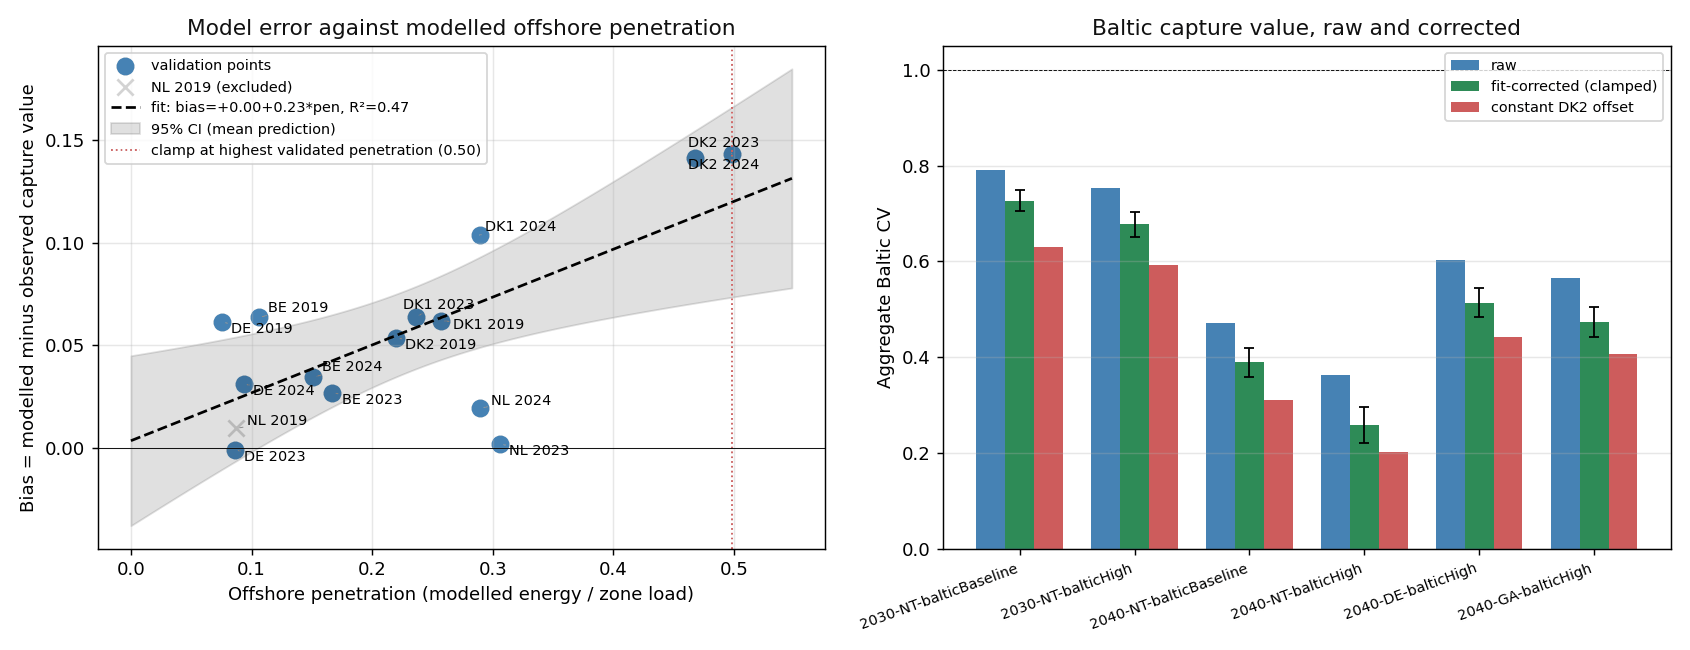
\includegraphics[width=0.95\textwidth]{fig_bias_fit_and_corrected}
    \caption{The bias correction and its effect: the validation bias against
    modelled penetration, anchored by DK2 (left), and raw against corrected
    Baltic capture value per scenario (right).}
    \label{fig:bias_corrected}
\end{figure}

The correction of Section~\ref{sec:bias_method} fits the model's capture-value
overstatement against its own offshore penetration on fourteen validation points
(five zones in 2019, 2023 and 2024, the Netherlands 2019 excluded). Only the two
DK2 entries lie above 31\,\% penetration, so the slope is a line between a
structureless low-penetration cloud and a single high-penetration zone
(Figure~\ref{fig:lozo}). Leave-one-zone-out makes this explicit
(Table~\ref{tab:lozo}): dropping any zone except DK2 leaves the slope between
0.22 and 0.28 with its 95\,\% interval clear of zero, while dropping DK2
collapses it from 0.233 to 0.045, sends the interval across zero, and drops the
penetration term's $R^2$ from 0.47 to 0.02. The penetration dependence is,
statistically, the statement that DK2 has a large bias at a high penetration.

The conclusion nonetheless survives, because the correction is not what produces
it. The uncorrected model already lands at 0.36--0.60 in 2040; the DK2-removed
correction is a near-constant offset of about 0.05 that takes it to 0.31--0.56;
the full correction reaches 0.26--0.51. All three agree on a loss of at least a
third of present capture value, and near half in the central scenario. DK2 is
kept as the anchor precisely because it
is the only existing high-penetration, Baltic-facing zone, which is what makes it
the right analogue and, at the same time, why the correction cannot be claimed as
a calibrated law. Reproduced by \texttt{1.19\_bias\_correction\_robustness.py}.

\begin{figure}[!htb]
    \centering
    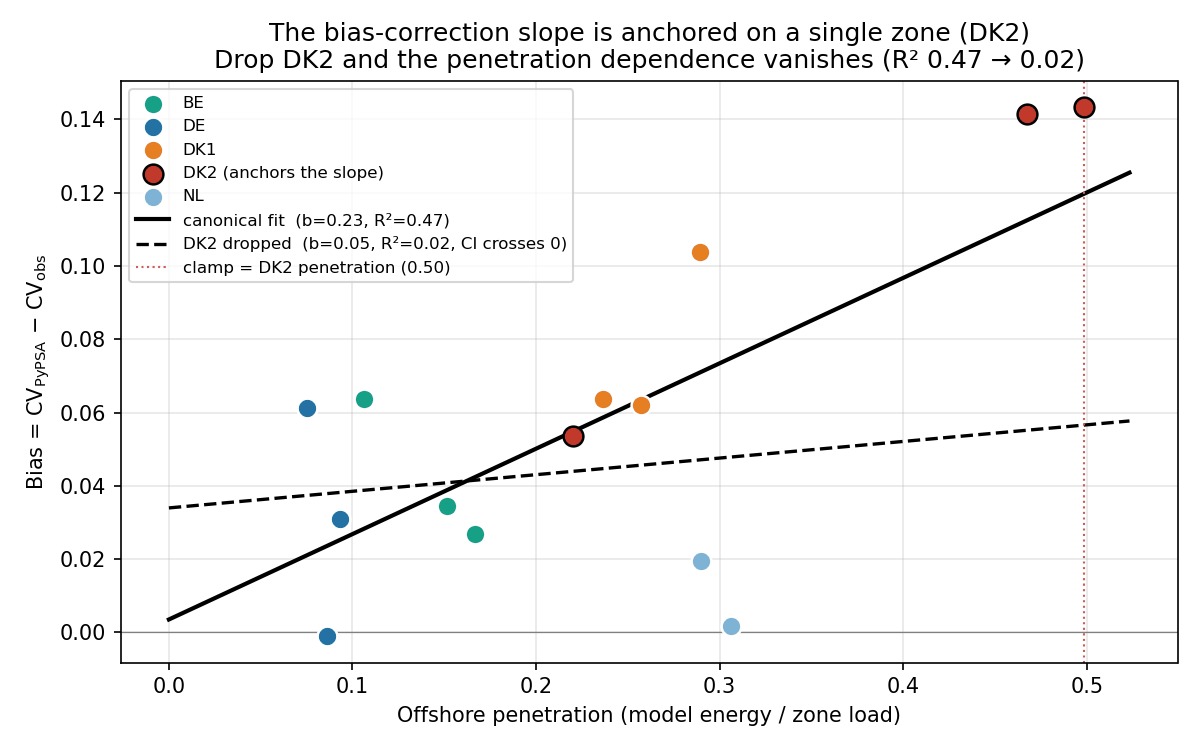
\includegraphics[width=0.8\textwidth]{fig_bias_lozo}
    \caption{The bias-correction slope is anchored on a single zone. The fourteen
    validation points (coloured by zone), the canonical fit, and the fit with DK2
    removed; without DK2 the penetration dependence vanishes ($R^2$ 0.47 to 0.02)
    and the slope's interval crosses zero.}
    \label{fig:lozo}
\end{figure}

\begin{table}[!htb]
\centering\small
\caption{Leave-one-zone-out and (last three rows) leave-one-year-out refits of
the bias slope. The slope and its 95\,\% interval are stable to dropping any zone
except DK2, whose removal collapses both.}
\label{tab:lozo}
\begin{tabular}{l c c c c}
\toprule
\textbf{Refit} & \textbf{$n$} & \textbf{Slope} & \textbf{95\,\% CI} &
\textbf{$R^2$} \\
\midrule
Canonical (all 14) & 14 & 0.233 & [0.08, 0.39] & 0.47 \\
Drop DE  & 11 & 0.262 & [0.05, 0.48] & 0.46 \\
Drop NL  & 12 & 0.278 & [0.18, 0.38] & 0.79 \\
Drop BE  & 11 & 0.251 & [0.06, 0.44] & 0.50 \\
Drop DK1 & 11 & 0.224 & [0.04, 0.40] & 0.46 \\
\textbf{Drop DK2} & 11 & \textbf{0.045} & \textbf{[$-$0.21, 0.30]} & \textbf{0.02} \\
\midrule
Drop 2019 & 10 & 0.303 & [0.11, 0.49] & 0.63 \\
Drop 2023 & 9 & 0.200 & [$-$0.00, 0.40] & 0.43 \\
Drop 2024 & 9 & 0.195 & [$-$0.04, 0.43] & 0.36 \\
\bottomrule
\end{tabular}
\end{table}


\subsection*{The DK2 price shape is outside the model class}

The bias correction treats the DK2 overstatement as a measured error. The
alternative, repairing the dispatch until DK2 comes out right, was tried
exhaustively and failed, which is what justifies the treatment
(Table~\ref{tab:dk2_experiments}). The blocking mechanism is structural: DK2
retains about 2,900~MW of export capacity into a Nordic system holding 62~TWh
of reservoir hydro, so a local surplus always finds a positive-priced sink and
the zonal price never collapses. The observed shape, 264 negative-price hours
in 2023, is produced by unit commitment, must-run combined heat and power, and
subsidised bidding, none of which a linear program contains.
Figure~\ref{fig:dk2_mechanism} shows the diagnosis: the model's generation is
right and its prices are too flat in exactly the windy hours. The model
that does land DK2 is the regression, out of fold at 0.798 against the
observed 0.784.

\begin{table}[!htb]
\centering\small
\caption{The DK2 re-dispatch experiments. No dispatch-side change
reproduces the observed 0.784; the shape needs mechanisms a linear program
does not contain. Values are DK2 capture value unless stated.}
\label{tab:dk2_experiments}
\begin{tabular}{p{3.6cm} p{4.4cm} p{5.6cm}}
\toprule
\textbf{Experiment} & \textbf{Change} & \textbf{Outcome} \\
\midrule
Faithful re-solve & none & 0.927 to 0.968: the price is not even unique \\
Negative wind bids & $-60$~\euro/MWh region-wide & no change: hydro absorbs the surplus \\
Derate the {\"O}resund alone & 3,396 to 1,700~MW & backfires: mean price 38 to 98~\euro/MWh, re-pinned to German gas \\
Myopic hydro & reservoirs capped at 24~h & explodes: 0.58 at a 1,207~\euro/MWh mean price \\
Market NTCs, both corridors & DK2--SE 1,700, DE--DK1 2,500~MW & DK1 error $+0.06$ to $+0.01$; DK2 unmoved at $+0.15$ \\
Rolling-horizon hydro & twelve monthly solves, 14-day lookahead & backwards: 0.932 to 0.957 \\
Must-run heat $\times$ negative bids (nine-point grid) & minimum load 0.20 to 0.50, bids 0 to $-10$~\euro/MWh & 0.947 to 0.958 across all nine; zero negative-price hours \\
\bottomrule
\end{tabular}
\end{table}

\begin{figure}[!htb]
    \centering
    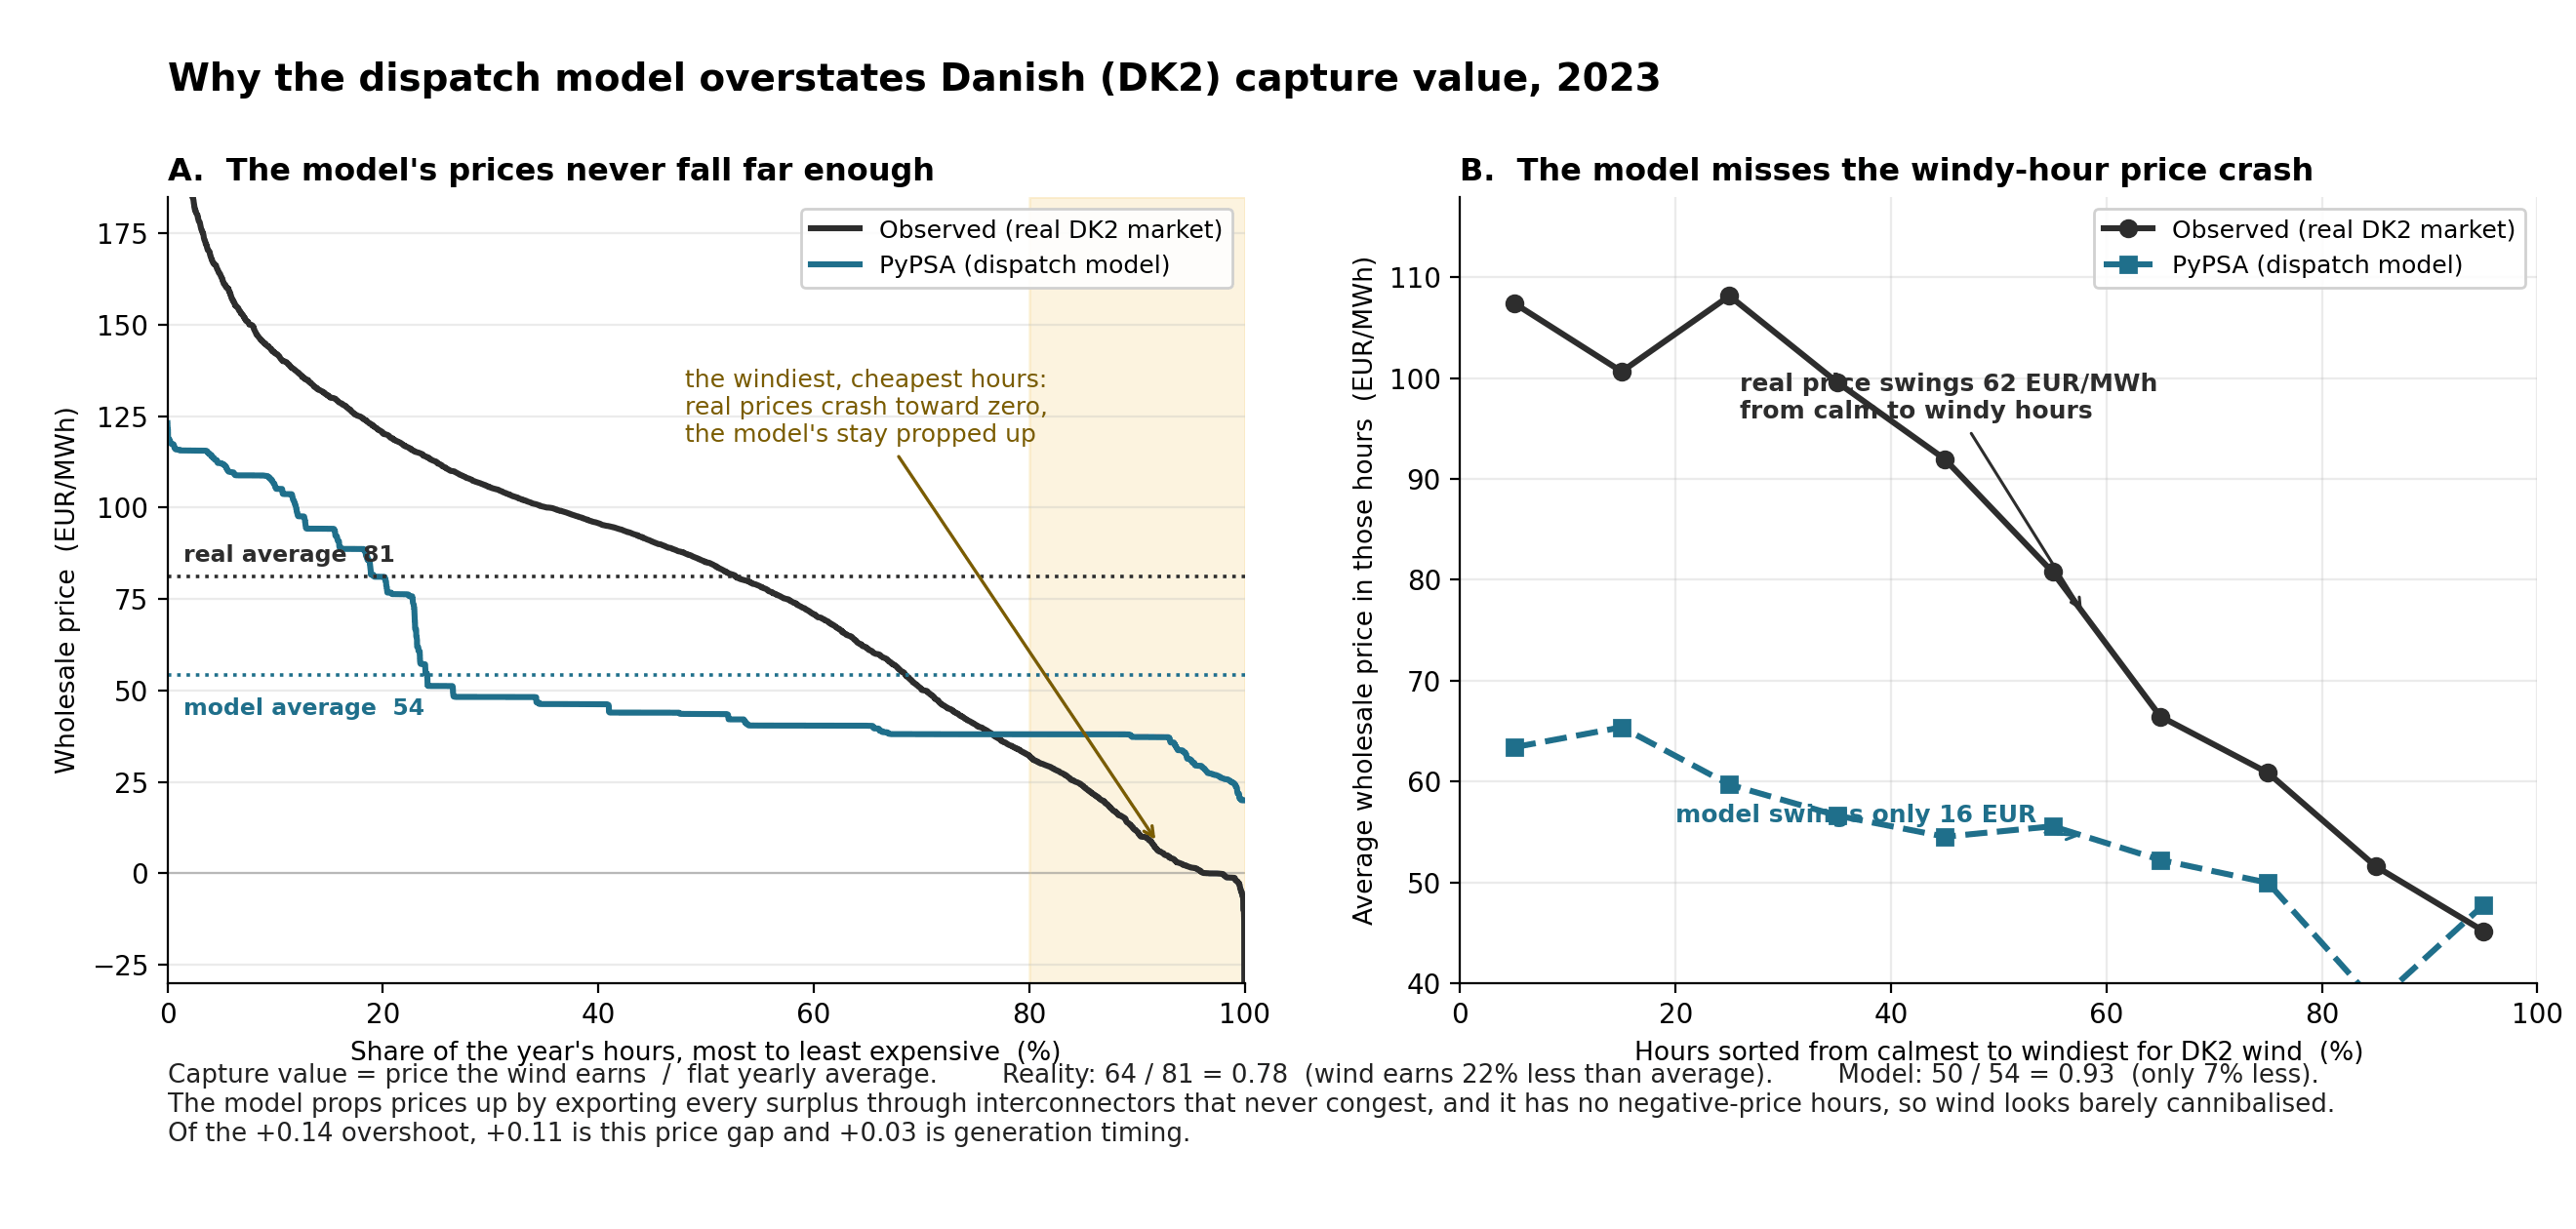
\includegraphics[width=0.9\textwidth]{fig_dk2_capturevalue_mechanism}
    \caption{The DK2 diagnosis. Pricing the model's own generation at observed
    prices recovers the observed capture value, so the wind is right and the
    error lives entirely in the price shape, which stays flat in the windy
    hours where real DK2 prices collapse.}
    \label{fig:dk2_mechanism}
\end{figure}

\subsection*{The hydrogen-demand assumption does not drive the result}

Correction D adds a parametric hydrogen layer that holds prices off zero at high
renewable shares; its demand is assumed, so the 2040 result is tested against it
by re-solving every 2040 scenario with the electrolyser demand and capacity
scaled to half and one-and-a-half times the canonical level
(Figure~\ref{fig:h2sens}). Across that $\pm 50\,\%$ range the energy-weighted
Baltic capture value moves by at most 0.013 in any scenario and by under 0.01 in
the two cannibalisation-dominated DE and GA scenarios; the 2040 band shifts only
from 0.36--0.60 at the central floor to 0.37--0.60 at either
extreme. Load-shed volumes are unchanged across the variants, so the small
sensitivity that does exist runs through the price floor and not through
adequacy: more hydrogen demand lifts the windy-hour prices where wind earns, so
capture value rises slightly. The floor sets the depth of the erosion at the
margin; it does not create it. Reproduced by
\texttt{1.20\_h2\_floor\_sensitivity.py}.

\begin{figure}[!htb]
    \centering
    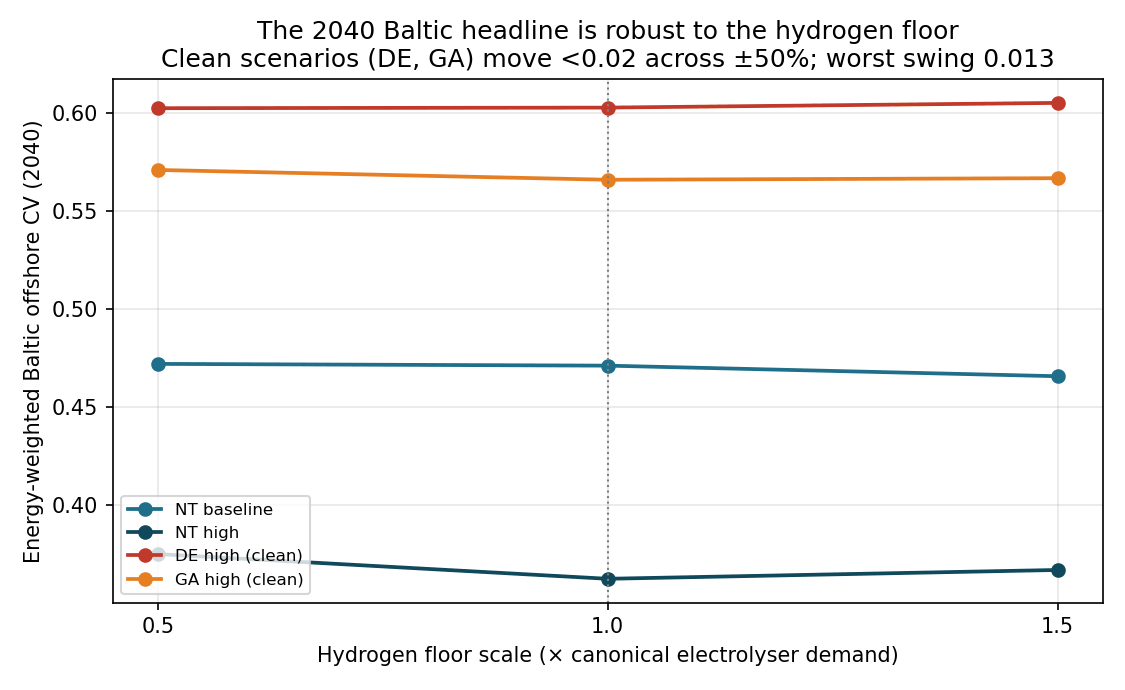
\includegraphics[width=0.8\textwidth]{fig_h2_sensitivity}
    \caption{The 2040 Baltic capture value against the scale of the assumed hydrogen demand (half to one-and-a-half times the
    central electrolyser demand). The clean
    DE and GA scenarios are nearly flat; the NT scenarios carry a small,
    floor-mediated dependence; the headline survives across the range.}
    \label{fig:h2sens}
\end{figure}

\subsection*{The gas-price grid}\label{sec:gas_results}

One input remains untested: the gas price that set every European record in 2022.
Re-solving three buildout scenarios across five gas prices, 15 to 120~\euro/MWh,
prices the exposure directly (Figure~\ref{fig:gas_cv}). The grid is coarse, fifteen networks, so the slopes indicate direction only. In 2030 the North Sea is the more exposed basin and the
Baltic is already near-decoupled: gas still sets the price often in the thermal
North Sea, rarely in the windy Baltic hours. Even end to end, the full crisis
sweep moves the 2030 North Sea capture value by only 0.07, less than one step of
the buildout. By 2040 both basins decouple almost entirely, their prices set by renewables, the demand-response tier, and hydrogen
production. Gas risk is real, asymmetric, and second-order. The buildout drives Baltic
value, and the fuel price only modulates it.

\begin{figure}[!htb]
    \centering
    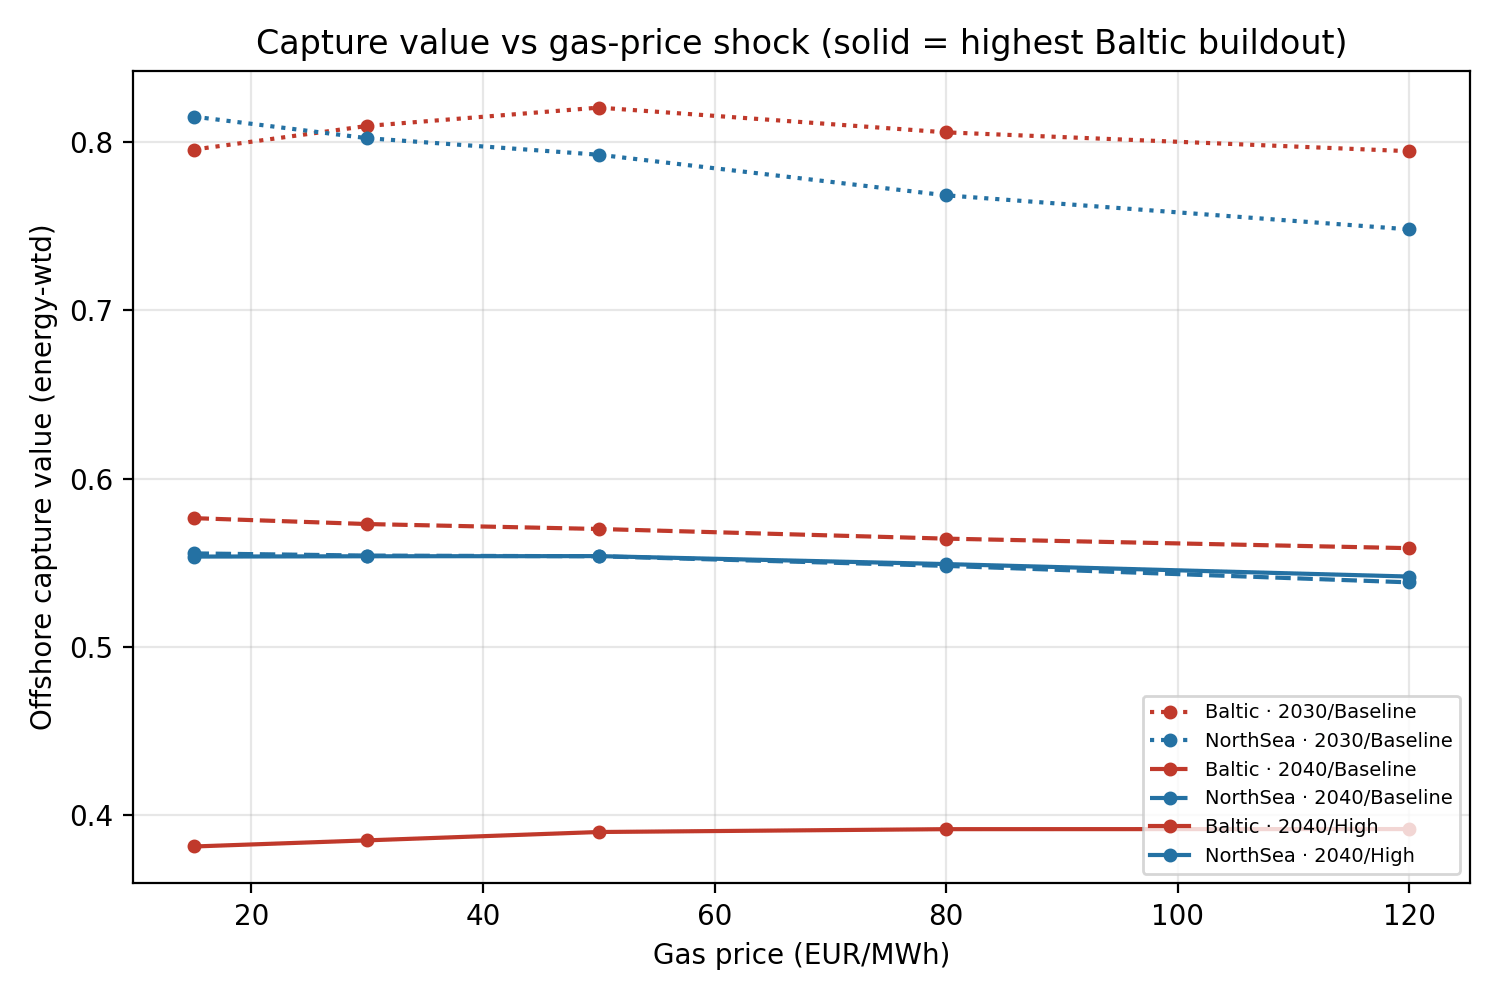
\includegraphics[width=0.92\textwidth]{fig_gas_shock_cv}
    \caption{Capture value across the gas-price grid, by basin and scenario. The
    North Sea's exposure is visible in 2030; the Baltic's curves are nearly flat,
    and by 2040 both basins decouple from gas.}
    \label{fig:gas_cv}
\end{figure}


\subsection*{The wider scenario sweep}

The fast approximation of the system model is a gradient-boosted model
trained on 76 solved networks
(the 55 dedicated training solves plus the 21 reused full-resolution baseline
and scenario solves of Table~\ref{tab:runs}), its inputs spread across the
scenario space by Latin hypercube sampling. Its training solves run
three-hourly; re-solving design points at full resolution confirms the
approximation is benign in the policy-relevant range and only optimistic at
the highest levels of buildout.

Its held-out skill is adequate for
exploration ($R^2$ 0.86 for capture value), it reproduces the 2040 scenarios to
within 0.05, and it leans optimistic beyond about 100~GW of Baltic offshore,
with the headline left to the direct solves throughout.

Across that space, buildout drives the erosion and gas barely moves it. The
Monte-Carlo draw (Figure~\ref{fig:montecarlo}), reaching beyond the plan to
150~GW, puts the median Baltic capture value at 0.28 and the
North-Sea-to-Baltic asymmetry near 2.3 times. The envelope samples
buildouts well beyond the official plans, to 150~GW, so its centre of mass is more
aggressive than any TYNDP scenario; that the direct solves sit in the upper half
of the distribution means the headline range is, if anything, conservative.
Nowhere in the explored space does heavy Baltic buildout coexist with a healthy
Baltic capture value.




\subsection{Weather-only corroboration}\label{sec:weather_agrees}

Features and capture values share market data, so the mechanism could be
circular. The weather is not. Clustering the farms by hourly output alone, no
prices and no market labels, the geography sorts them on its own
(Figure~\ref{fig:clusters}): North Sea zones correlate at 0.44, the
under-built Baltic states at 0.61, the built-out DK2 and SE4 at 0.87, and the
two basins are largely independent at 0.28. The grouping reflects meteorology,
and it points forward: the under-built zones, the ones the buildout will fill,
are a tightly-correlated bloc. The same signal
repeats inside countries: a compact fleet blows nearly as one (Belgium 0.96,
Poland 0.94) while a spread one does not (Germany 0.64, Denmark 0.67).
Germany's farms even split into a North Sea and a Baltic block, so the basin is the right boundary for the analysis (Appendix~\ref{app:supplementary}). The physical picture behind the
enclosure penalty is now complete: Baltic wind arrives together, into a smaller market with weaker export capacity.

\begin{figure}[!htb]
    \centering
    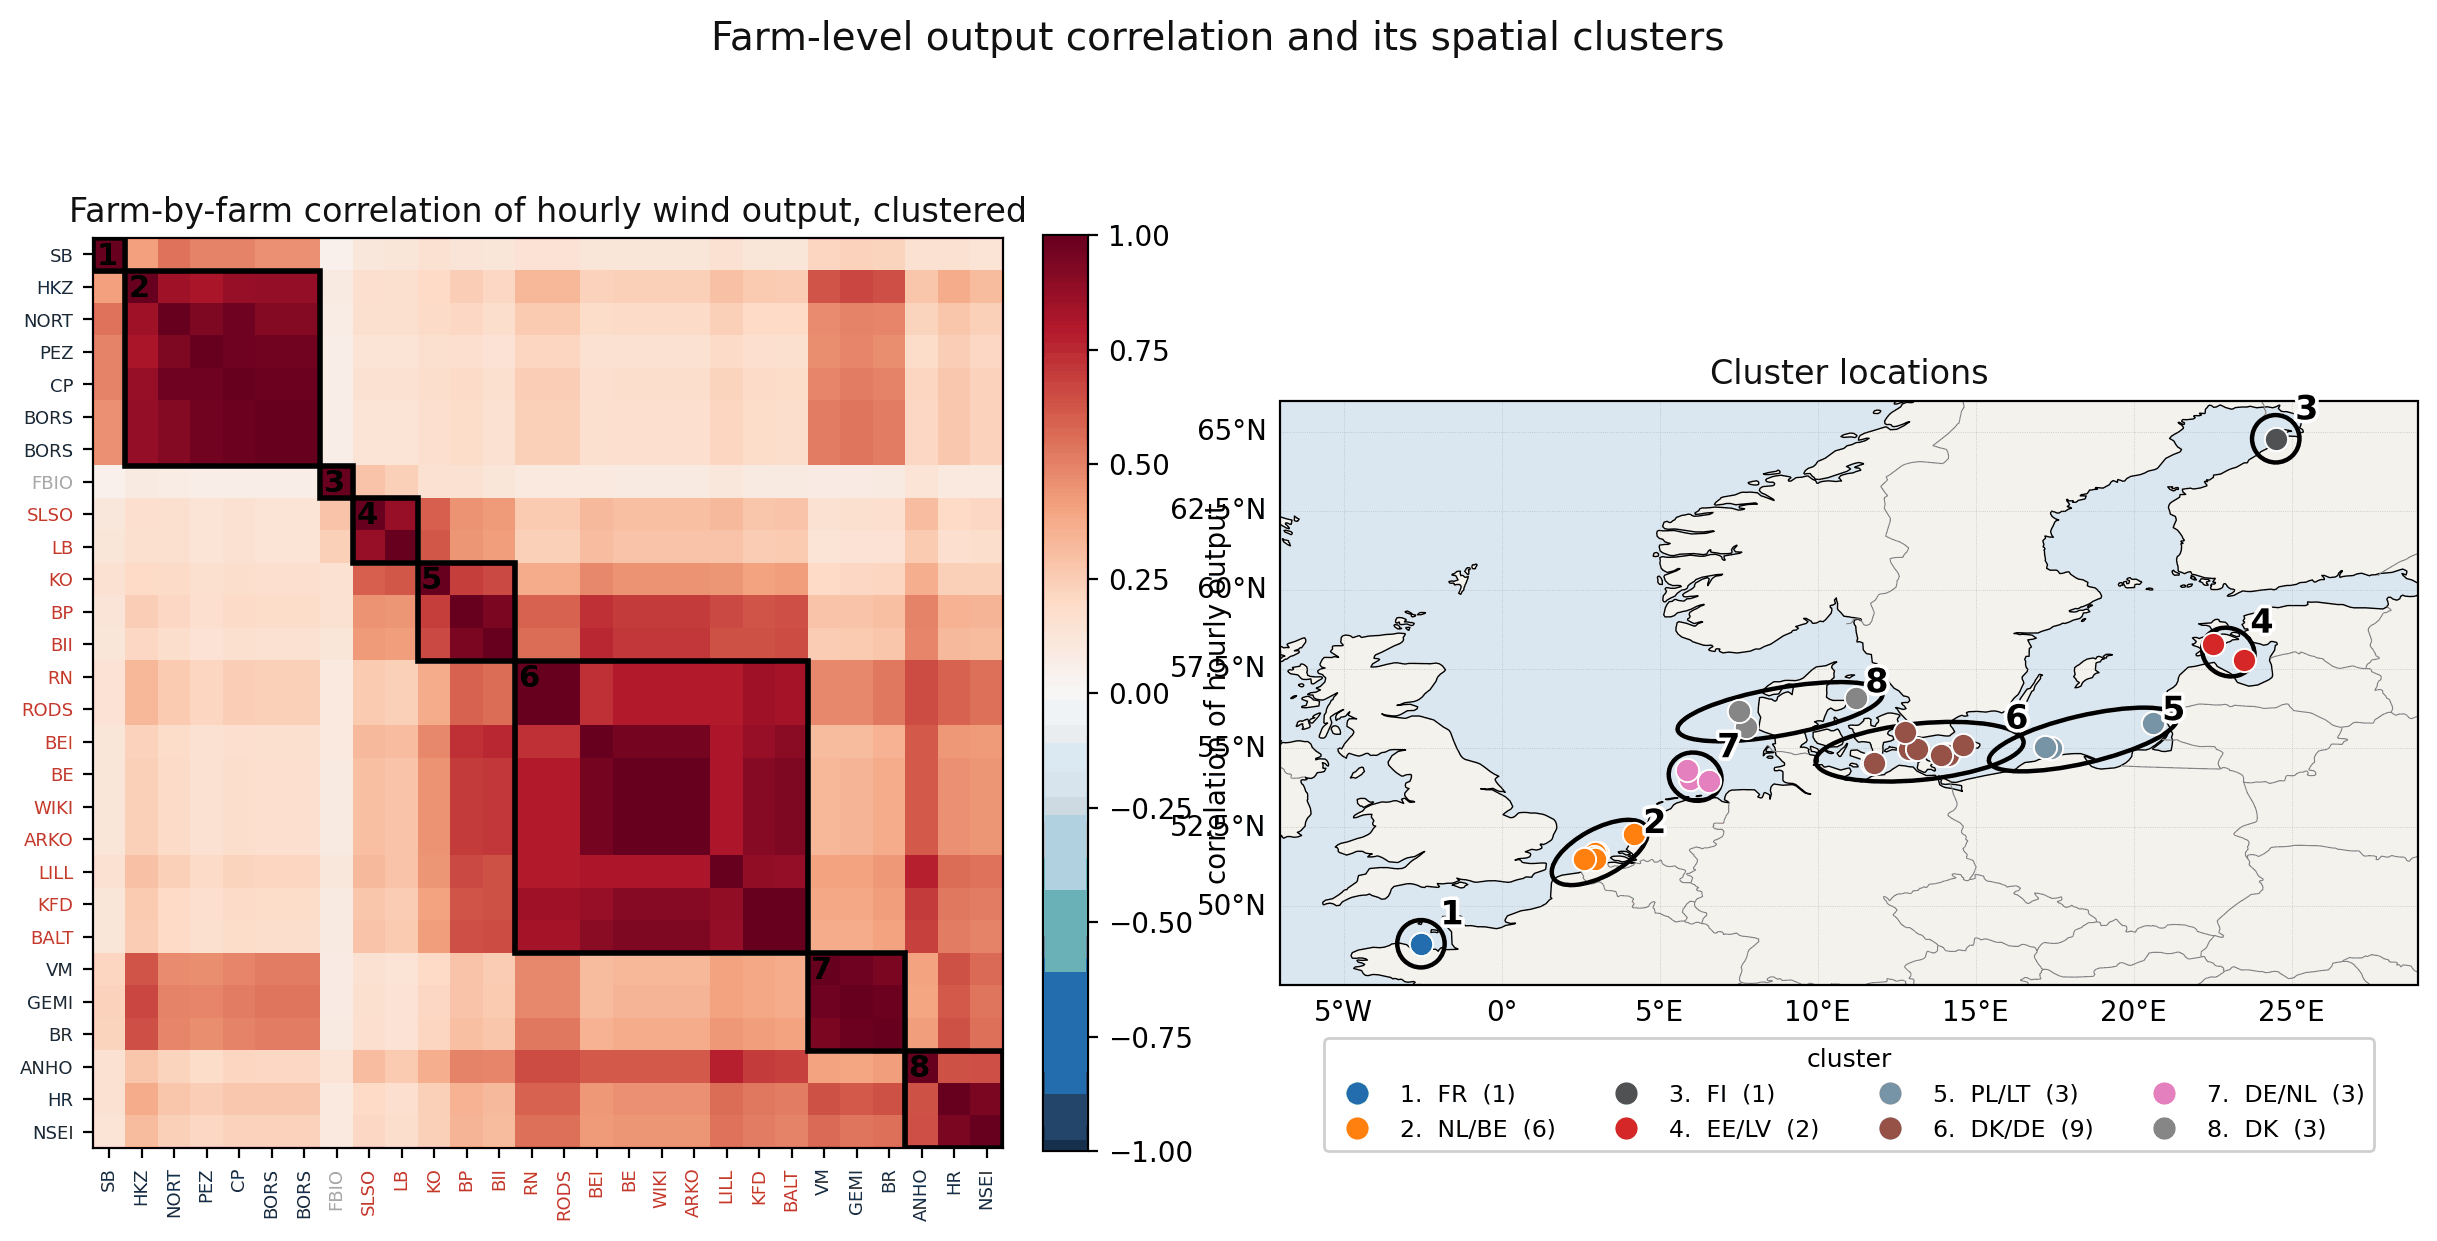
\includegraphics[width=0.98\textwidth]{fig_basin_correlation}
    \caption{Weather-only corroboration: hourly-output correlation clustered
    (left) and the clusters mapped (right). Within-basin correlation is high
    and cross-basin low: North Sea 0.44, under-built Baltic 0.61, built-out
    0.87, cross-basin 0.28.}
    \label{fig:clusters}
\end{figure}

That proximity reflects the mechanism itself. Plotting every farm pair's
output correlation against its separation collapses both basins onto a single
decay curve, correlation falling away with a fitted length of 422~km
(Figure~\ref{fig:corr_distance}). The Baltic pairs obey no different physics;
they sit on the near, steep end of the same curve because the basin's farms
are closer together (median 285~km against 347, a few long pairs
notwithstanding).
Distance sets synchronicity, and the Baltic's geography fixes the distance.

\subsection{Scarcity and gas sensitivities}\label{sec:scarcity_results}

The second movement begins by ruling out the rival explanations. Could the
2040 erosion be adequacy stress rather than cannibalisation?
Recomputing every capture value with scarcity-priced hours removed answers it
(Figure~\ref{fig:scarcity_bars}): the 2030 and clean 2040 scenarios barely
move, and the two NT scenarios, whose $+0.15$ adequacy component sits almost
entirely in Poland, still reach only 0.51 to 0.62,
far below today's 0.88. The floor of the range comes from cannibalisation alone.

Gas is the other suspect input, and it is second-order too. Re-solving three
buildouts across five gas prices, 15 to 120~\euro/MWh, moves the 2030 North
Sea capture value by only 0.07 end to end, less than one step of the buildout.
By 2040 both basins have decoupled from gas almost entirely, their prices set by renewables, demand response and hydrogen production
(Appendix~\ref{app:robustness}). Baltic value is set by the buildout, with fuel prices a second-order
influence.

\subsection{Sector coupling and flexible demand}\label{sec:sector_results}

The grid is the spatial escape for surplus wind; the temporal escape, heat,
hydrogen and storage absorbing windy hours locally, is excluded from the
electricity-only model by construction. A sector-coupled variant therefore
tests it against an electricity-only twin identical in every setting
(Section~\ref{sec:sector_method}), so the difference between the two solves
is the value of flexibility alone.

\begin{table}[!htb]
\centering
\caption{The value of flexible demand: the matched twelve-hour 2040 solves,
    TYNDP fleet pinned, frozen grid. Zero-price columns give the share of wind
    energy produced into zero-priced hours.}
\label{tab:sector}
\begin{tabular}{l c c c c}
\toprule
& \multicolumn{2}{c}{\textbf{Capture value}} &
\multicolumn{2}{c}{\textbf{Zero-price share}} \\
\textbf{2040 solve (12\,h)} & \textbf{North Sea} & \textbf{Baltic} &
\textbf{NS} & \textbf{Baltic} \\
\midrule
Electricity only & 0.51 & 0.54 & 45\,\% & 29\,\% \\
Sector-coupled   & 0.74 & 0.82 & 19\,\% & 25\,\% \\
Flexibility effect & $+0.23$ & $+0.28$ & & \\
\bottomrule
\end{tabular}
\end{table}

Flexibility recovers most of what the frozen grid destroys
(Table~\ref{tab:sector}): the isolated effect, $+0.23$ and $+0.28$, is the
same order as the grid lever, and it is again the Baltic that gains most,
ending above the open basin as local electrolysis absorbs its surplus. In 2030
the sector world sits within a few points of the electricity-only one, so
flexibility, like transmission, pays only once the erosion binds. Per-zone
values are in Appendix~\ref{app:tables}.

Two facts keep the headline in place: the zero-price problem shrinks but does
not vanish, 19 to 25\,\% of wind energy still unpaid in the sector-coupled
solves, so the contract question survives full flexibility; and the
twelve-hour resolution smooths the price shape both arms see, so these
numbers bracket the hourly headline rather than replace it. Read beside the two grid solves, the levers agree: the frozen electricity-only world is the
floor, and either escape lifts the Baltic off it further than the North
Sea.

\FloatBarrier
% ----------------------------------------------------------------------------


\subsection{Pricing scarcity}\label{sec:scarcity_method}

A stressed scenario must be able to not serve demand, and the price of that
choice shapes every average. Correction F sets the ladder, demand response at
five percent of peak load offered at 400~\euro/MWh and unserved energy at the
4,000~\euro/MWh cap, so scarcity hours price as the real market would, and
Section~\ref{sec:robustness} measures how much of each scenario's erosion is
scarcity rather than cannibalisation.

\subsection{The sector-coupled variant}\label{sec:sector_method}

The electricity-only model can move surplus wind only through space, over the
grid; real systems also move it through time and into other demands. To measure how much of the projected erosion flexible demand removes, the
system model is rebuilt in PyPSA-Eur's sector-coupled configuration,
heating, hydrogen, storage and electric transport co-optimised alongside
electricity for an overnight 2040 system. The full-sector problem is tractable
only at twelve-hour resolution, so its control is an electricity-only twin
solved at the same twelve hours with every other setting identical, both arms
pinned to the same TYNDP fleet, so the difference between the two solves is
the value of flexibility itself. Two limits qualify the reading: twelve-hour
steps smooth the price shape both arms see, and country-level pinning makes
small zones such as DK2 incomparable across arms
(Section~\ref{sec:sector_results}).

\section{The Two-Estimator Test}\label{app:two_estimators}

Section~\ref{sec:gap_decomposition} states why the two models diverge beyond
the observed record. This appendix carries the underlying test, which asks
whether the divergence follows from how each model is built rather than from
any disagreement about how prices form. The error types named here are
structural descriptions of each model's construction; the measured composition
of each model's error, on held-out targets, is the Theil partition reported in
Section~\ref{sec:skill}.


The division of labour has a mathematical basis, and it was tested
(Figure~\ref{fig:theory}). The regression is a bounded interpolator: four
hundred trees give a piecewise-constant surface whose output cannot leave the
training range and whose gradient is exactly zero outside it. The system
model is a linear program whose price is the shadow price of the nodal energy
balance, re-derived from the merit order every hour with no training range at
all, but floored at zero. Table~\ref{tab:error_anatomy} sets the two error
structures side by side.

\begin{table}[!htb]
\centering\small
\caption{The two error structures compared. Each row is measured in this
chapter or Appendix~\ref{app:robustness}; the mean signed errors are against
observed 2023--24 capture values.}
\label{tab:error_anatomy}
\begin{tabular}{p{3.2cm} p{5.3cm} p{5.3cm}}
\toprule
 & \textbf{Regression model} & \textbf{System model} \\
\midrule
Error type & Bounded interpolation & Simplified market \\
Mean signed error & $-0.005$ & $+0.057$ \\
Sign and shape & No systematic sign & Always overstates; grows with
congestion \\
Largest where & Outside the training support (all 36 projection rows) & Small,
hydro-coupled zones (DK2 $+0.14$) \\
Detected by & Range and convex-hull checks & Three-way comparison \\
Consequence & Returns a constant from 2040 & Corrected by the measured fit \\
\bottomrule
\end{tabular}
\end{table}

Three consequences follow, and the runs confirm each
(Table~\ref{tab:theory_numbers}). Outside the range of its training data the regression model returns a
constant: across the four Baltic 2040 scenarios its answers span 0.008 of
capture value where
the system model spans 0.43, a fifty-four-fold difference. The two agree
where both can be checked, to 0.06 in sample and 0.04 at 2030, and diverge to
0.35 at 2040, where the projection leaves the training support. And the
system model's error has a predictable sign and order: it overstates every
validated zone, most where zones are small and hydro-coupled, DK2 above DK1
above Belgium above Germany and the Netherlands, which is exactly the shape
the bias correction of Section~\ref{sec:bias_method} subtracts.

One expectation fails, and the failure is informative. The erosion was
expected to accelerate with penetration; the fitted response is the opposite,
a saturating curve, because the zero price floor caps how much a marginal
windy hour can still lose once the price already sits at zero. The saturation
means the system model, if anything, understates cannibalisation at extreme
penetration, so the 2040 numbers are upper bounds on capture value,
conservative in the same direction as the measured bias. The two models' errors are of different kinds, and the division of roles
places each model where its error is smallest. Section~\ref{sec:skill} measures
those kinds directly on held-out targets.

\begin{figure}[!htb]
    \centering
    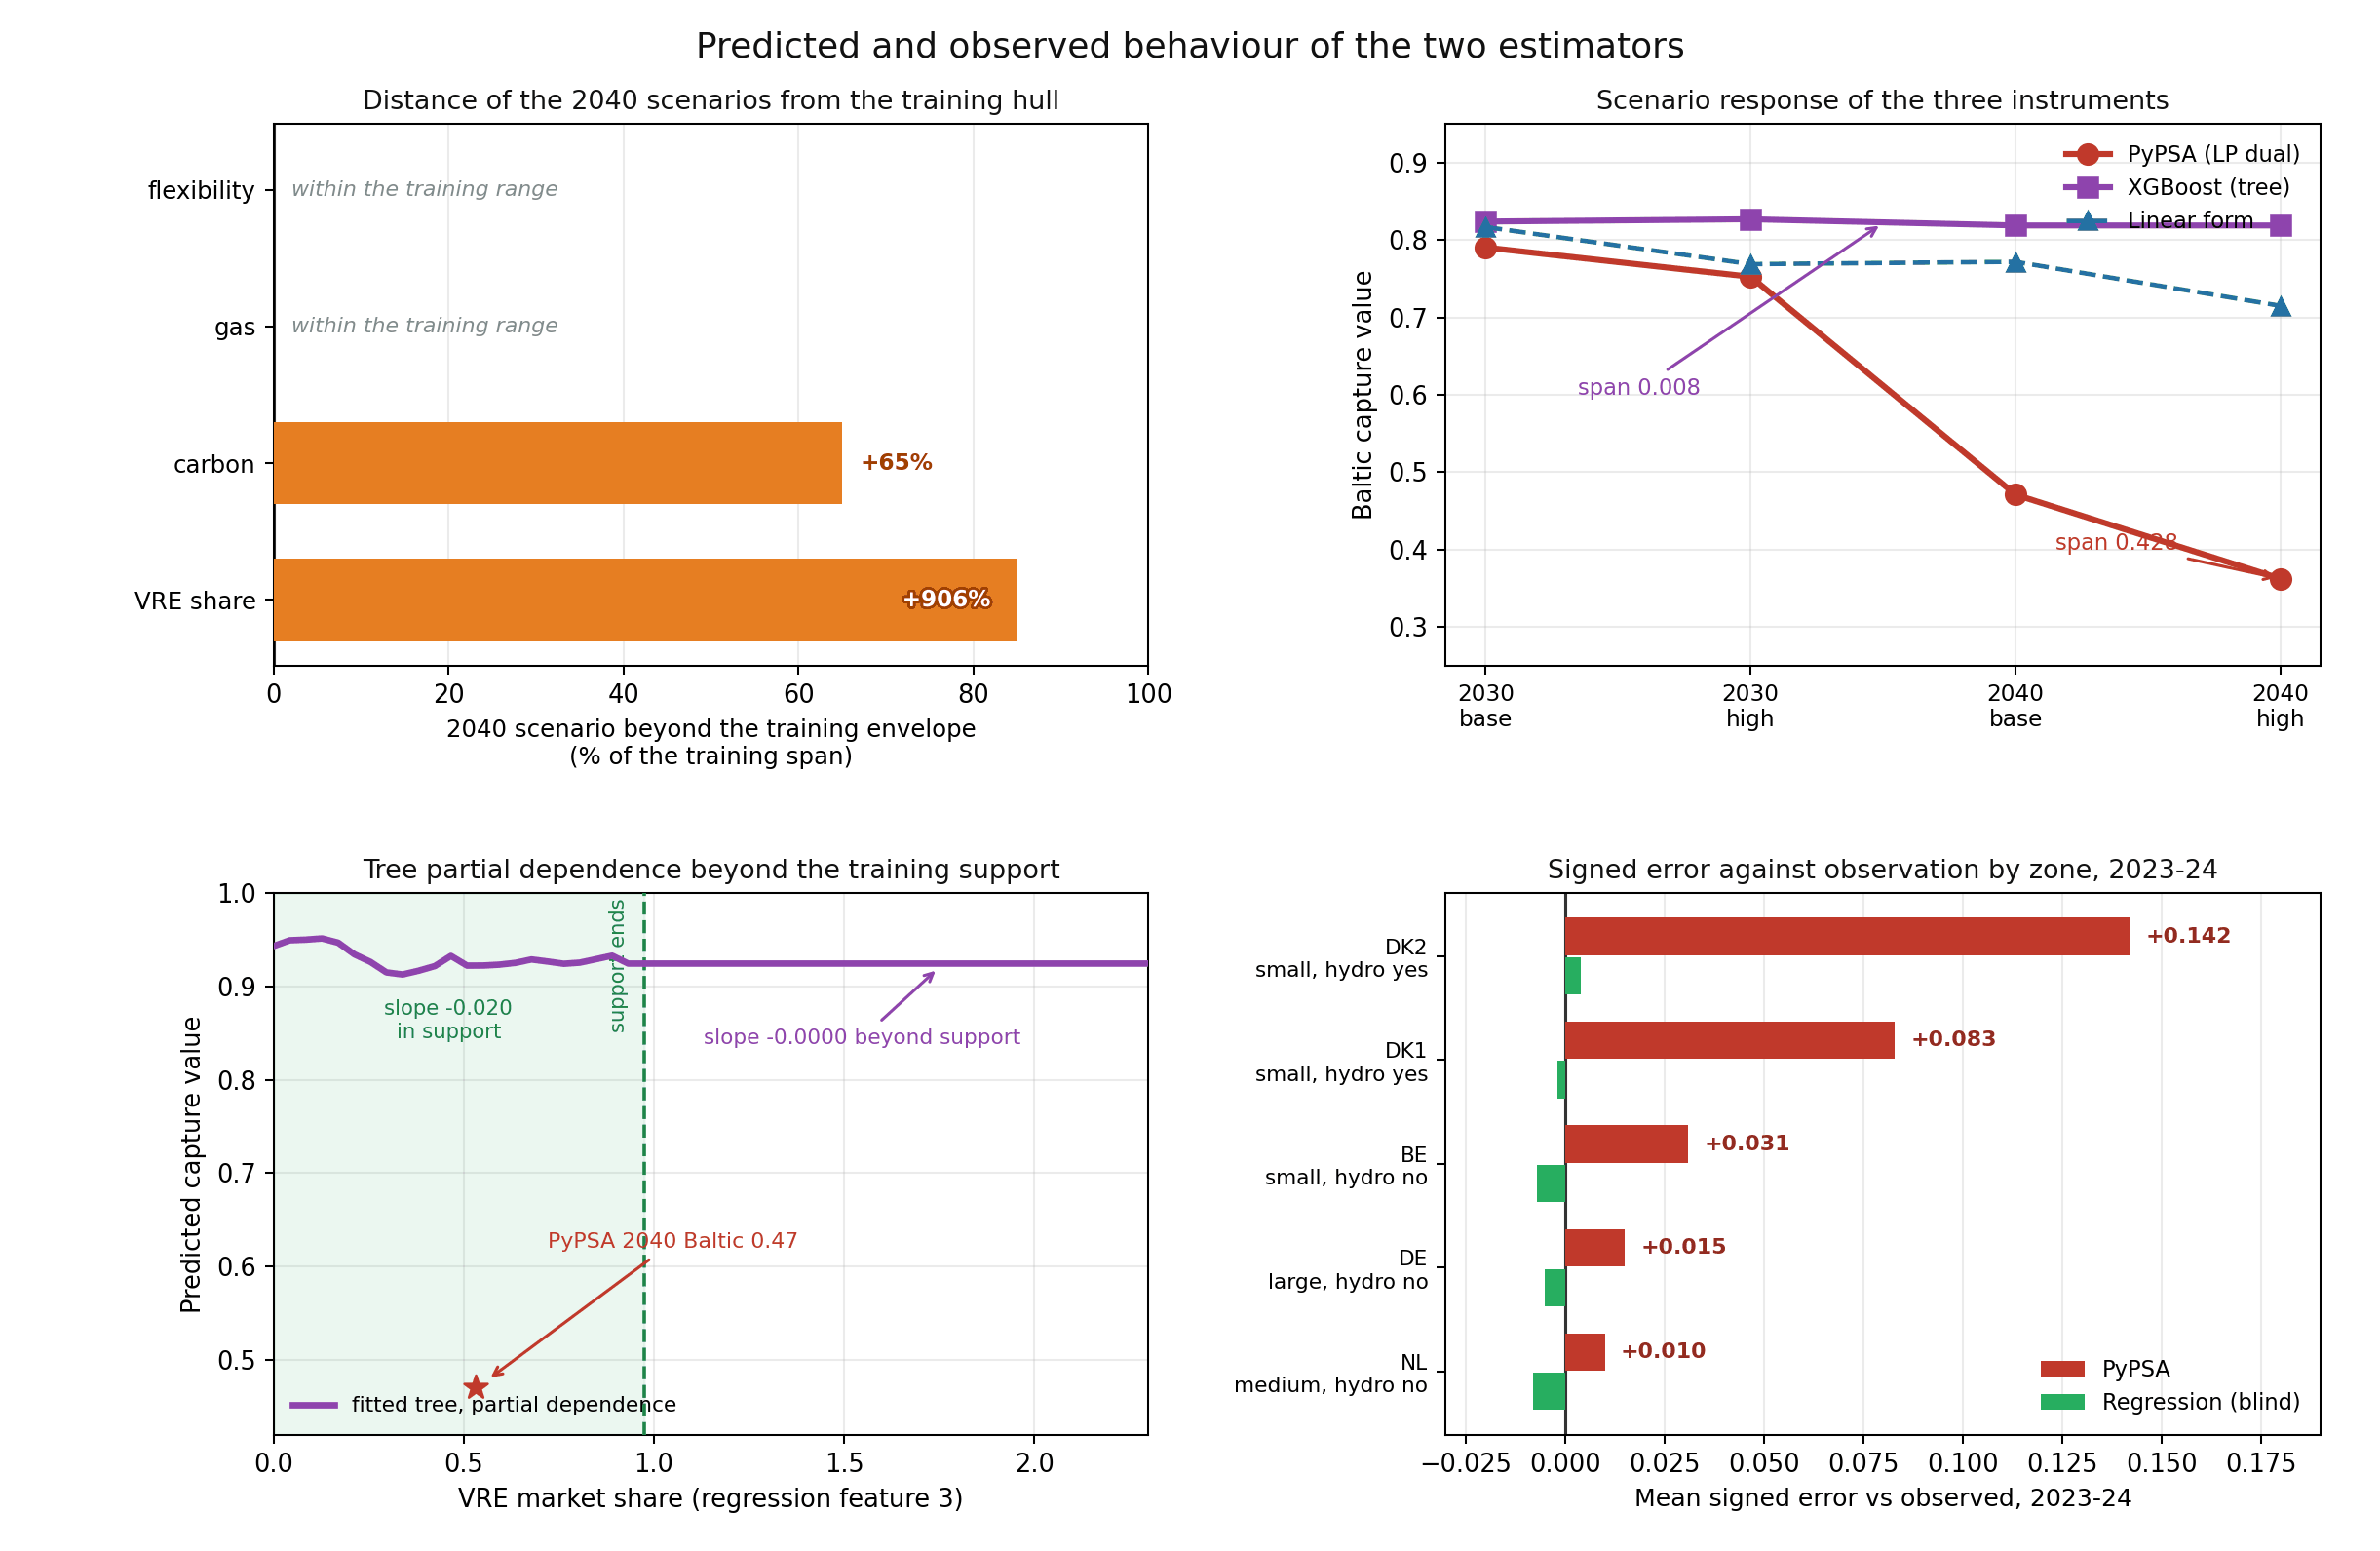
\includegraphics[width=0.95\textwidth]{fig_theory_vs_evidence}
    \caption{Why the models must differ, tested against the runs. Top
    left: every 2040 scenario leaves the training envelope, renewable share
    furthest. Top right: across the four Baltic scenarios the tree moves 0.008
    where the system model moves 0.43. Bottom left: the tree's fitted response
    is exactly flat beyond its support, so the divergence comes from leaving the range of the training data and does
    not reflect curvature. Bottom right: the system model's in-sample error is largest
    in small, hydro-coupled zones, the regression's is near zero, which fixes
    the sign and order of the bias correction.}
    \label{fig:theory}
\end{figure}

\begin{table}[!htb]
\centering\small
\caption{The two-estimator test in numbers. Response spans are across the four
Baltic 2040 scenarios; divergence is the mean absolute gap between the
models' Baltic estimates; curvature is the fast-approximation fit across 76 solved
networks with a cluster-bootstrap interval; errors are against observed
2023--24 capture values.}
\label{tab:theory_numbers}
\begin{tabular}{l >{\raggedright\arraybackslash}p{7.9cm}}
\toprule
Response span: tree / linear / analytical / system model & 0.008 / 0.102 / 0.179 / 0.428 \\
Divergence: in sample / 2030 / 2040 & 0.062 / 0.035 / 0.348 \\
Penetration-squared coefficient (95\,\% CI) & $-0.193$ [$-0.215$, $-0.169$]: concave \\
Mean signed error: system / regression & $+0.057$ / $-0.005$ \\
System error by zone & DK2 $+0.14$ > DK1 $+0.08$ > BE $+0.03$ > DE $+0.02$ > NL $+0.01$ \\
\bottomrule
\end{tabular}
\end{table}
\FloatBarrier

\FloatBarrier

\section{Portfolio and Distributional Analyses}\label{app:portfolio}

These analyses serve Objective~5 and the question of who bears the loss. They
are reported here in full; their conclusions are carried in
Sections~\ref{sec:site_ranking} and~\ref{sec:one_figure}.

\subsection{Spreading across both basins}\label{sec:diversification}

Objective~5 asks whether allocating capacity across both basins beats
concentrating it in the North Sea; the two channels of
Section~\ref{sec:mitigation} are tested separately because they give opposite
answers (Figure~\ref{fig:diversification}).

\begin{figure}[!htb]
    \centering
    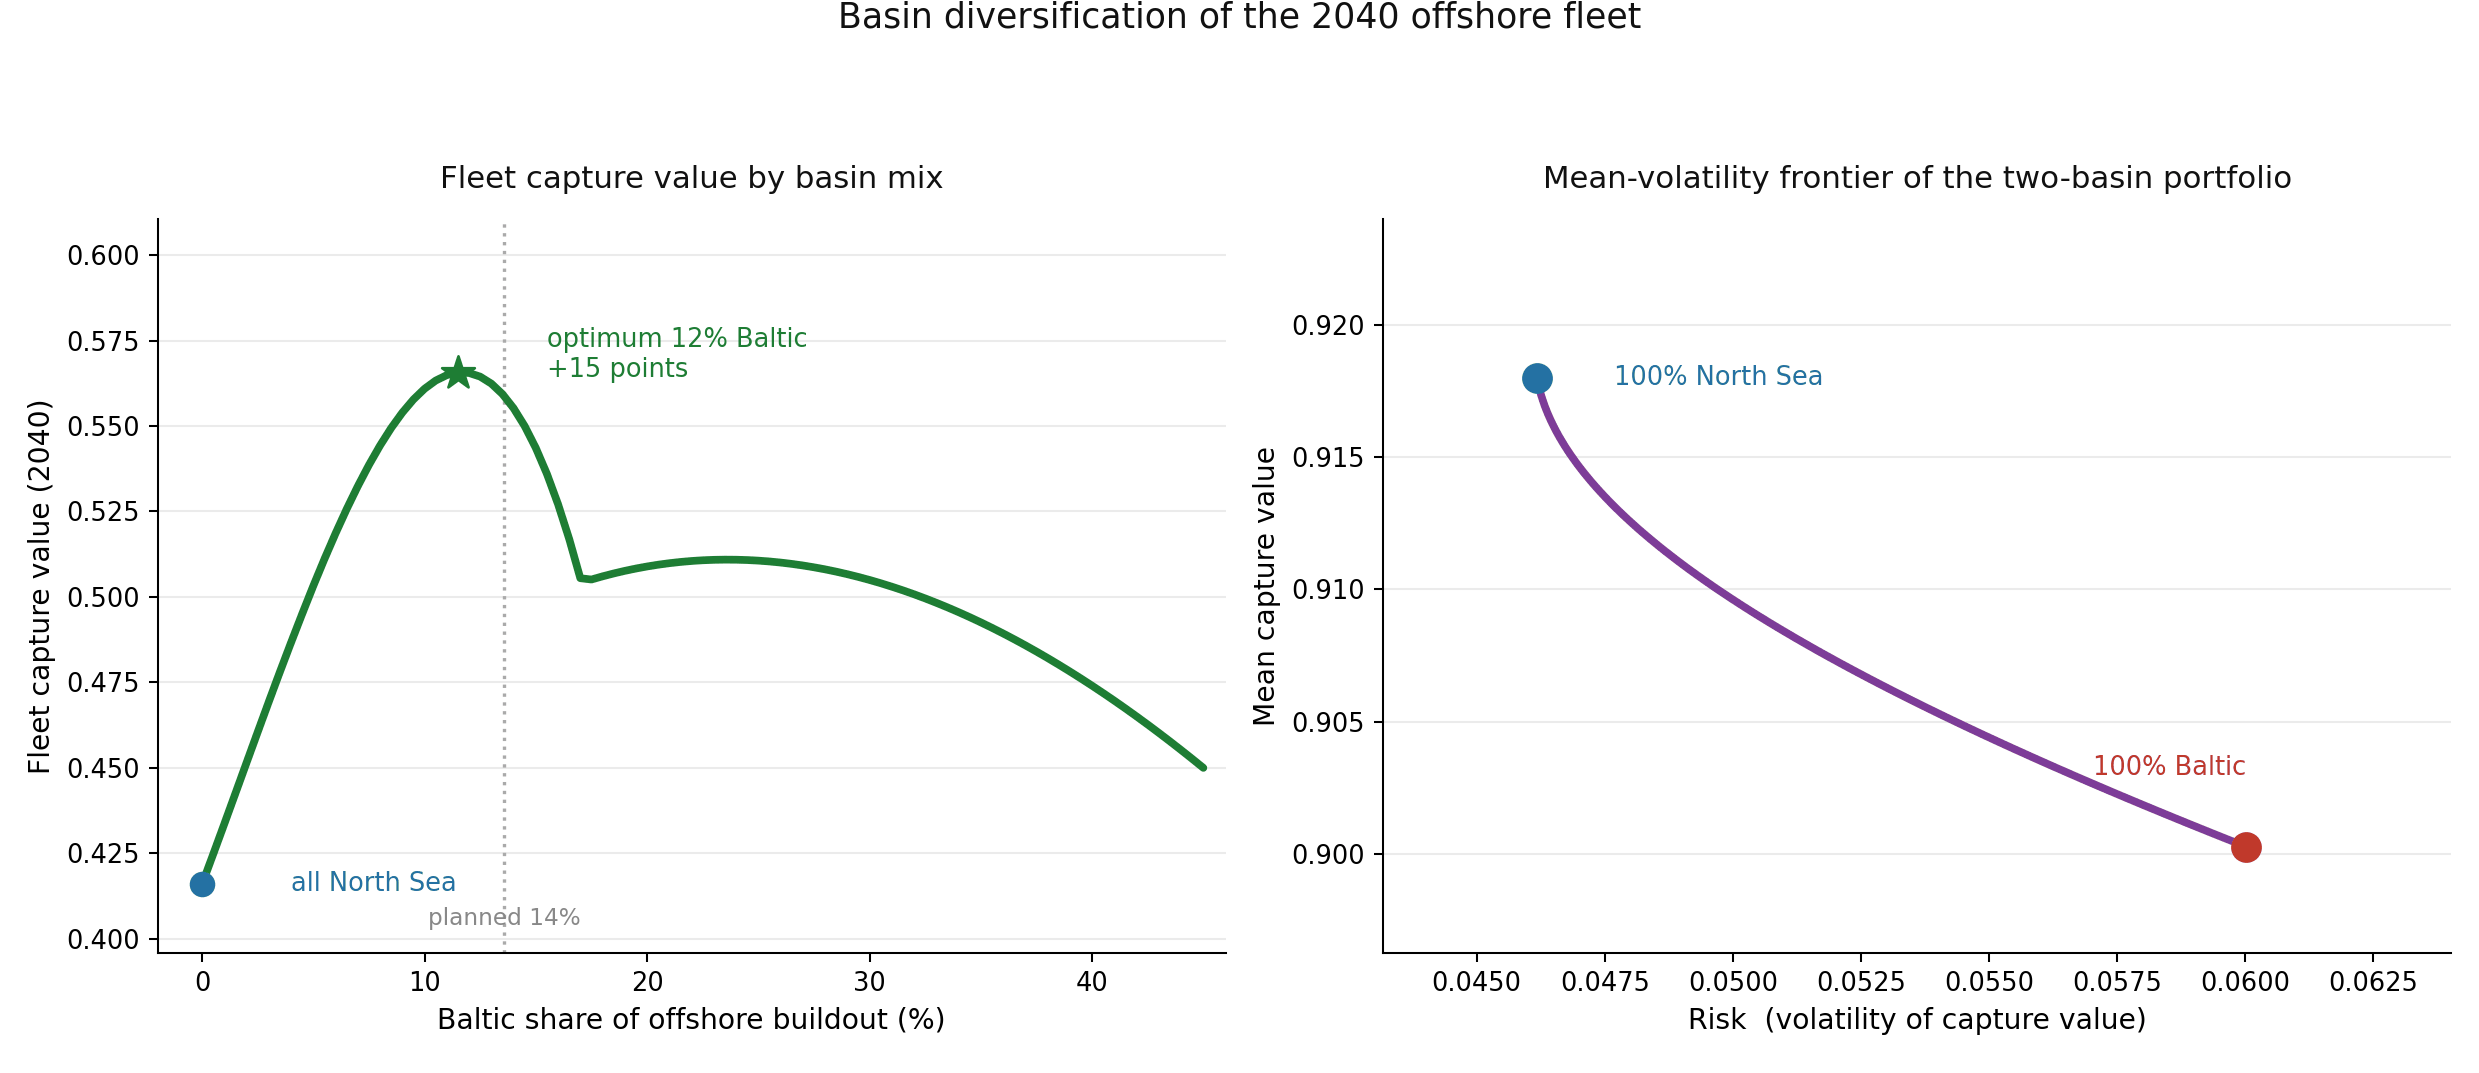
\includegraphics[width=0.94\textwidth]{fig_diversification}
    \caption{The two portfolio channels. Left: aggregate 2040 capture value of a
    fixed 623~TWh of offshore generation as a function of the share allocated to
    the Baltic, holding the total constant. Right: the mean-variance frontier
    built from monthly capture values, 2017 to 2024. Spreading the fleet raises
    the mean but does not reduce the variance.}
    \label{fig:diversification}
\end{figure}

The first channel is a cannibalisation hedge, and it works. Holding total
offshore generation fixed and varying only its split, an all-North-Sea
allocation cannibalises itself down to an aggregate capture value of 0.416,
while shifting 12\% to the Baltic, which starts earlier on its curve, lifts
the aggregate to 0.566, a gain of 36\%; the planned 14\% split is within
half a point of that optimum.

The second channel is a risk hedge, and it fails. Monthly capture values
over 2017 to 2024 make the North Sea simultaneously the higher-mean and
lower-variance basin (0.918 at 0.046 against 0.900 at 0.060), and the two
series co-move at a correlation of 0.80, so the minimum-variance portfolio
is 100\% North Sea and spreading delivers no volatility reduction at all.

The 0.28 wind correlation of Section~\ref{sec:mechanism} explains the split:
wind is decorrelated, so moving capacity eases cannibalisation, but market
coupling propagates price levels across borders. The benefit of spreading
sits entirely in the mean: the portfolio is less cannibalised, while its
volatility barely changes.

% ----------------------------------------------------------------------------
\subsection{Method: decomposing capture value by price state and pricing congestion rent}\label{app:whopays_method}

\subsubsection*{Who bears the loss: decomposing capture value by price
level}\label{sec:whopays_method}

A capture value states how much revenue is lost. It does not state who loses it,
and under the support instruments reviewed in
Section~\ref{sec:mitigation} the answer differs by mechanism. A two-sided
contract for difference tops any positive price up to the strike, and volumes
constrained off by the network are compensated under Article~13 of Regulation
(EU) 2019/943 \cite{EURegulation2019943}, so both losses fall on the state. In a
zero or negative price hour the contract is suspended, following GB practice from
allocation round four and the 2024 market design reform
\cite{EUMarketReform2024}, so that loss falls on the farm and no compliant
scheme may cover it. What decides the bearer is therefore the price \emph{level},
not the physical cause.

Capture value factorises to match. Writing $z$ for the share of generation
occurring in hours priced below a threshold $\epsilon$, and $\mathrm{CV}^{+}$ for
the capture value computed over the remaining hours,
%
\begin{equation}
    \mathrm{CV} = (1 - z)\,\mathrm{CV}^{+},
    \qquad\text{so}\qquad
    \underbrace{1 - \mathrm{CV}}_{\text{total loss}}
    = \underbrace{z}_{\text{farm-borne}}
    + \underbrace{(1-z)\bigl(1 - \mathrm{CV}^{+}\bigr)}_{\text{state-borne}}
    \label{eq:whopays}
\end{equation}
%
and the split is exact, with nothing left over. The farm-borne term is energy earning
nothing with the contract suspended; the state-borne term is the depression of
positive prices that the contract absorbs. Both are computed hour by hour on the solved networks for
2030 and 2040 under the frozen and cost-optimal grids, with
$\epsilon = 1$~\euro/MWh. Because the linear program floors prices at zero
(Section~\ref{sec:pypsa_how}), $z$ is a conservative lower bound on the real
farm-borne share, which in a market with a negative-price tail would be larger.
Curtailed volume is reported separately, since it never enters capture value at
all yet is compensated under the same Article~13. The observed anchor is the
wind-weighted share of 2023 and 2024 generation falling in hours with a
day-ahead price at or below zero. A required strike price, $\mathrm{LCOE}/(1-z)$,
follows directly and states what a contract must pay if the farm is to recover
its costs given that a share $z$ of its output earns nothing.

\subsubsection*{Congestion rent and who funds the
remedy}\label{sec:rent_method}

If interconnection is the lever, its affordability is a fair question, and the
income that congestion itself generates is the natural place to look. For every
branch the rent is the flow multiplied by the price difference across it, summed
over the year:
%
\begin{equation}
    R_{\ell} = \sum_{t} w_t \, f_{\ell,t}
    \bigl( \eta_{\ell}\,\lambda_{\mathrm{to}(\ell),t} - \lambda_{\mathrm{from}(\ell),t} \bigr)
    \label{eq:congestion_rent}
\end{equation}
%
with $f_{\ell,t}$ the flow, $\lambda$ the nodal prices, $w_t$ the snapshot
weighting, and $\eta_{\ell}$ the efficiency, which is unity for lossless lines
and the link efficiency for controllable interconnectors. Rents are aggregated by
border and classified by whether each branch is internal to a basin or crosses
its boundary. The same quantity is computed on the frozen and the cost-optimal
network, so that the difference measures the rent that building the grid
destroys, which is the merchant-transmission problem Joskow and Tirole
\cite{JoskowTirole2005} identify. Against that income sits the annualised capital cost of the transmission the optimal solve builds, taken as the added
capacity multiplied by its annuitised cost. Because frozen-grid Poland prices
several hundred scarcity hours, every rent figure is reported twice, once over
all hours and once excluding hours above 390~\euro/MWh, the same threshold used
for the scarcity sensitivity in Section~\ref{sec:scarcity_method}. The comparison must not be added to the captured-revenue gain of
Section~\ref{sec:vlcoe_grid_method}: both arise from the same price convergence,
and building the lines removes the rent, so the two must not be summed.

\subsection{Who bears the loss, and what funds the cure}\label{sec:whopays_results}

Every number so far has said how much value is lost; who loses it is a
separate question with a different answer. Applying the factorisation of Equation~\ref{eq:whopays} splits
each basin's erosion into the part a contract absorbs and the part it cannot;
Figure~\ref{fig:whopays} draws that split for both basins and both grids.

\begin{figure}[!htb]
    \centering
    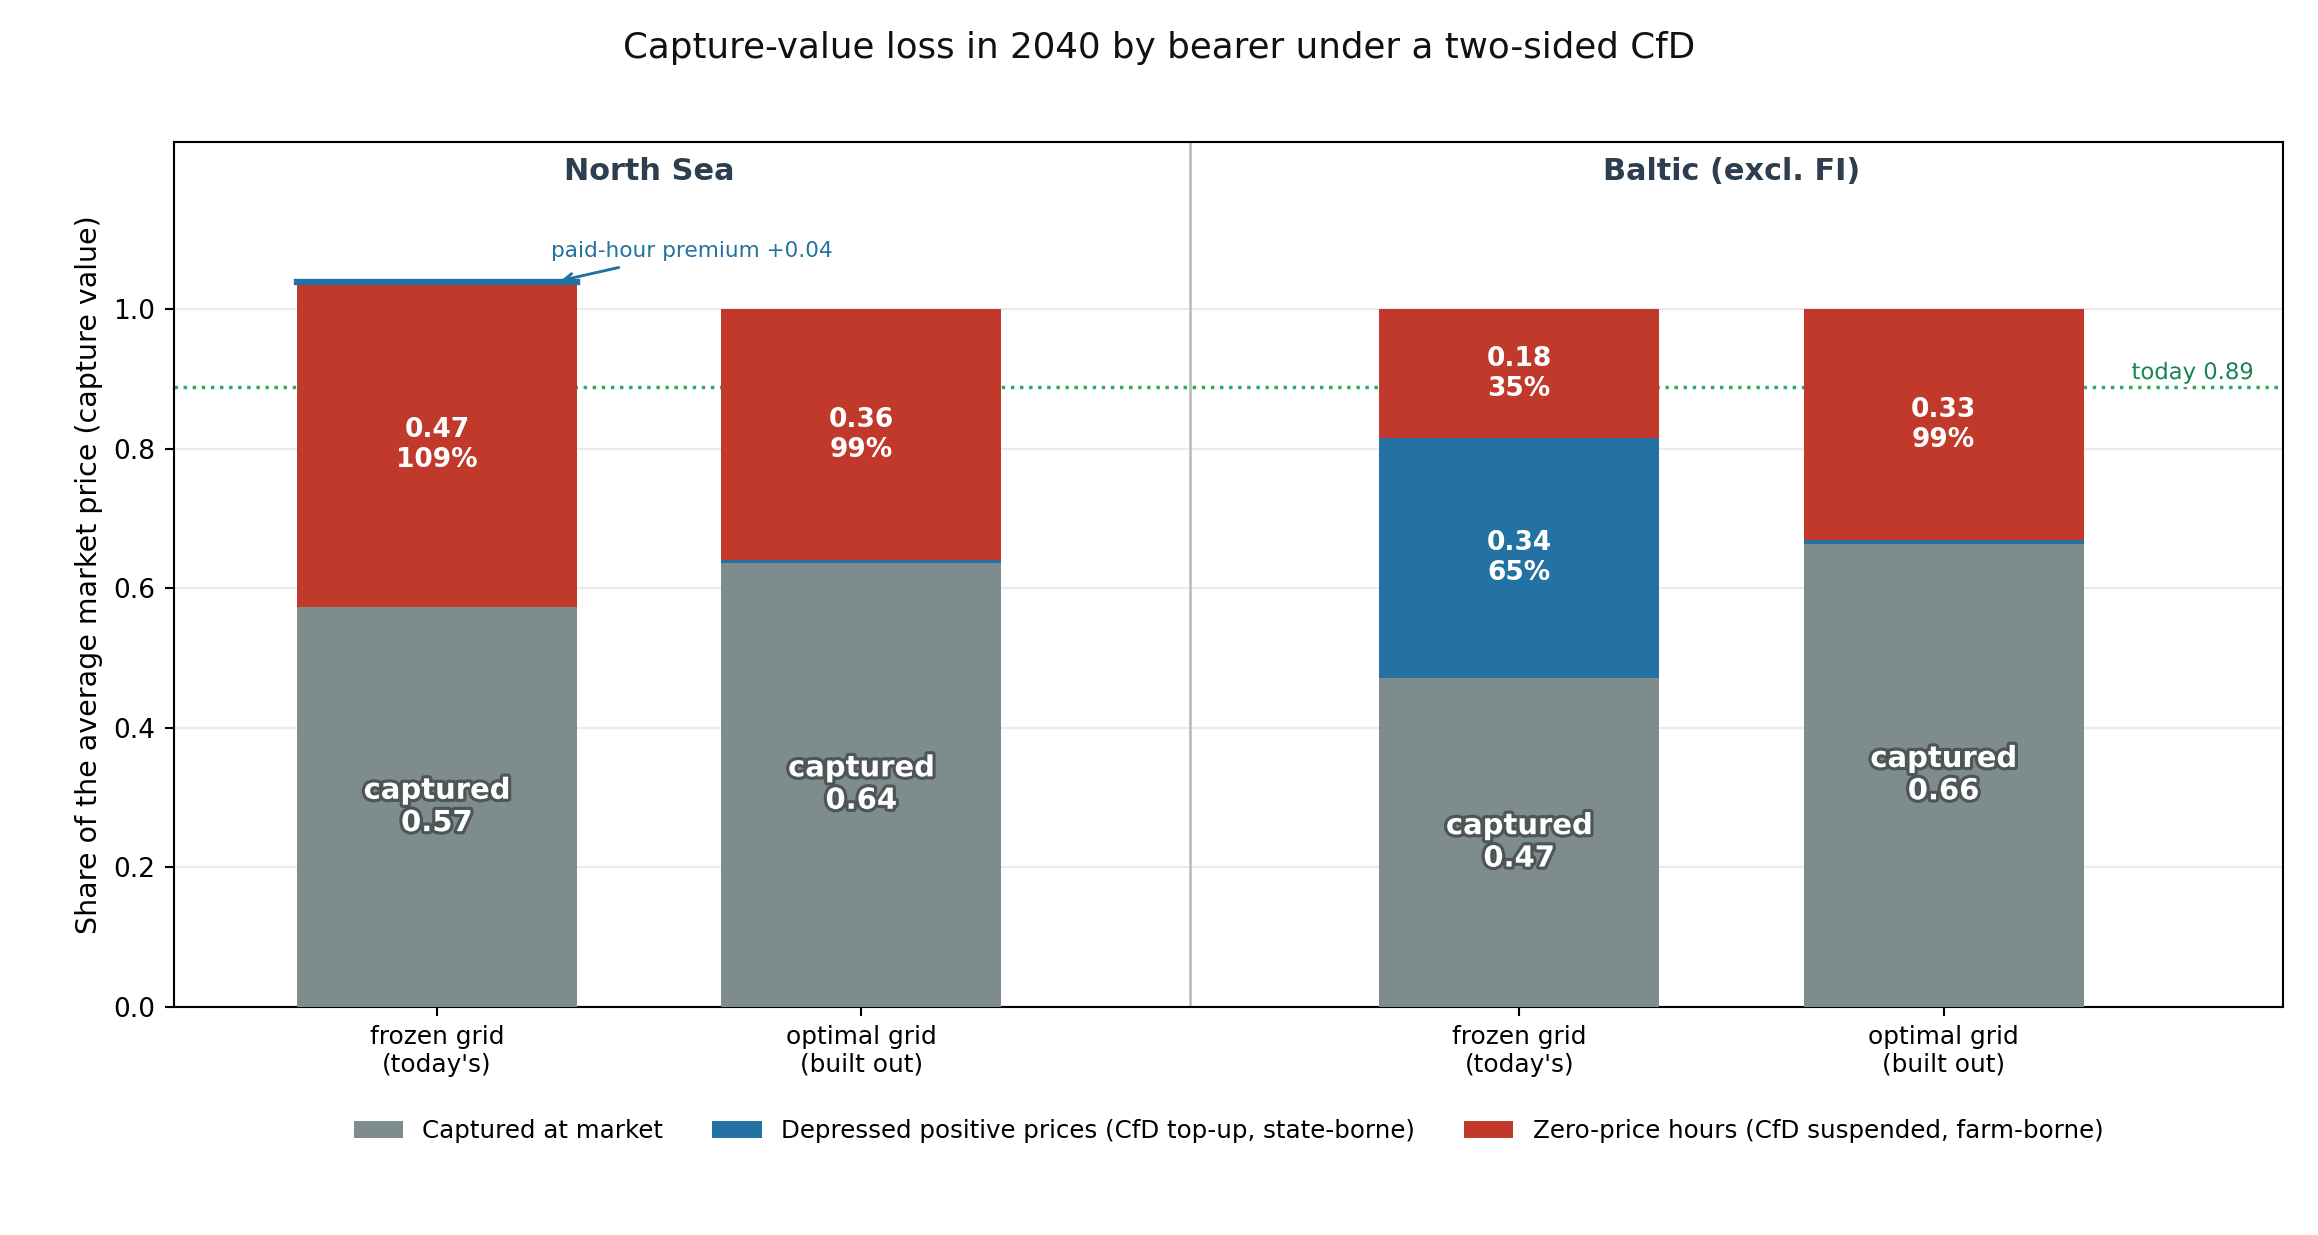
\includegraphics[width=0.94\textwidth]{fig_whopays_decomposition}
    \caption{The 2040 capture-value loss split by bearer. The grey block is
    revenue captured at market. The blue block is value lost to depressed but
    positive prices, which a two-sided contract tops up to the strike, so the
    state carries it. The red block is energy earning nothing, where the contract
    is suspended and the farm carries it. In the frozen North Sea the paid hours
    earn a small premium ($+0.04$), which offsets part of the zero-price loss,
    so the farm-borne share amounts to 109\% of the net loss.}
    \label{fig:whopays}
\end{figure}

The two basins look similar on the capture-value chart and are opposites
underneath it. The frozen-grid Baltic factorises as
$(1-z)\,\mathrm{CV}^{+} = 0.815 \times 0.578$:
only 18.5\% of its energy earns nothing, so almost two-thirds of its loss is
depressed-but-paid, the kind a contract absorbs. The North Sea factorises as
$0.533 \times 1.075$: its paid hours earn slightly above average, so there is
no depression to top up and the entire loss is uncompensable; with
$\mathrm{CV}^{+}$ above one the state term is a small premium, so the farm's share slightly exceeds the loss itself. The basin with the worse
headline number has the better protected investor.

Volume shows the same split from the other side: the frozen-grid North Sea
spills a third of its available 2040 energy against 3.6\% in the Baltic,
curtailment being a further state-borne bill invisible to capture value.

Building the grid does not simply reduce the loss, it changes its bearer.
Under optimal expansion the depression factor snaps to about 0.99 in both
basins, so what survives is purely the zero-price channel: the share of Baltic
energy earning nothing \emph{rises} from 18.5\% to 33.1\% even as capture
value improves, because interconnection couples the basin to the wider
system's surplus hours, and roughly 99\% of the remaining loss becomes
farm-borne: a fiscal problem converted into an investor one, a consequence
absent from the transmission-benefit literature.

The zonal detail separates three regimes the basin averages hide
(Appendix~\ref{app:tables}): scarcity-priced Poland, the locally oversupplied
eastern Baltic, and the open North Sea, most exposed but most relieved. The
strike a contract needs follows the same split, $\mathrm{LCOE}/(1-z)$,
roughly 71~\euro/MWh for Poland against 125 to 210 across the open zones,
converging to 92 to 103 under expansion: an ordering that inverts the
capture-value ranking for a contract-backed investor.

All farm-borne shares here are conservative: the linear program floors prices
at zero, and the observed 2023 to 2024 anchors already show 5.9\% of North
Sea and 3.0\% of Baltic generation at or below zero, so the real exposure is
larger than reported.

% ----------------------------------------------------------------------------
\subsubsection{Congestion rent and the cost of the cure}\label{sec:rent_results}

The recommendation that follows is to build transmission, and its
affordability need not be a public spending question: congestion is itself a
revenue stream, and Article~19 of Regulation (EU) 2019/943 already earmarks
that revenue for this purpose \cite{EURegulation2019943}.
Equation~\ref{eq:congestion_rent} prices it. The rent accrues to the transmission operators, and none of it reaches
generators: congestion is only ever a cost to a wind farm, and the question here is only whether the
system's own congestion income covers the cure.

\begin{table}[!htb]
\centering
\small
\caption{Annual congestion rent in 2040, in billion euro per year, computed on
the frozen and cost-optimal networks. Figures are given over all hours and
excluding scarcity hours above 390~\euro/MWh, since frozen-grid Poland prices
several hundred such hours. The grid cost is the annualised capital cost of all
transmission the cost-optimal solve builds across the fourteen countries.}
\label{tab:congestion_rent}
\begin{tabular}{l r r}
\toprule
 & \textbf{All hours} & \textbf{Excluding scarcity} \\
 & (bn\euro{} per year) & (bn\euro{} per year) \\
\midrule
System congestion rent, frozen grid & 38.9 & 22.6 \\
\quad of which Baltic-related & 11.8 & 4.3 \\
System congestion rent, optimal grid & 15.2 & 15.1 \\
\quad of which Baltic-related & 2.1 & 2.1 \\
\midrule
Rent destroyed by building the grid & 23.7 & 7.4 \\
Annualised capital cost of the new lines & 2.7 & 2.7 \\
\midrule
\textbf{Baltic rent as a multiple of total grid cost} & \textbf{4.4$\times$} & \textbf{1.6$\times$} \\
\bottomrule
\end{tabular}
\end{table}

The conservative column is the one to quote: even excluding every scarcity
hour, Baltic-related borders generate 4.3~bn\euro{} per year against an
annualised 2.7~bn\euro{} for the entire fourteen-country expansion. The
enclosed basin already produces, and by statute already earmarks, more than
enough income to pay for the interconnection that would relieve it, and the
concentration is specific: the German-Polish border alone carries
7.2~bn\euro{} on the frozen grid. Poland's borders are where the money and
the constraint coincide.

Two qualifications matter. First, the rent and the captured-revenue gain
must not be added: building the lines destroys the rent that funds them, the
merchant transmission problem in its original form \cite{JoskowTirole2005},
so the rent is the pre-existing, ring-fenced funding pool and the welfare
gain the justification. Second, expansion is not congestion-free: Baltic
\emph{border} rent collapses from 2.9 to 0.7~bn\euro{} while \emph{internal}
rent barely moves, so interconnection resolves the enclosure and leaves the
domestic bottlenecks standing.

% ----------------------------------------------------------------------------

\section{Forecast Checks on the Two Models}\label{app:forecast_checks}

Each model's mean squared error is separated following Theil \cite{Theil1966}:
\begin{equation}
\mathrm{MSE} = \underbrace{(\bar{\hat y}-\bar{y})^{2}}_{\text{bias}}
+ \underbrace{(s_{\hat y}-s_{y})^{2}}_{\text{variance}}
+ \underbrace{2(1-r)\,s_{\hat y}s_{y}}_{\text{covariance}},
\label{eq:theil}
\end{equation}
whose three shares sum to one.


Section~\ref{sec:backtest} states the conclusions of two checks on the models
as forecasters. This appendix carries them in full.

\subsection{Backtesting the act of projecting}

Skill on held-out targets tests the models but not the projection, which
additionally has to build its future inputs. The one horizon where that whole
chain can be scored is the recent past: fitted on data to 2021 and asked for
2023 and 2024, across the same four zones, ninety-six zone-months
(Table~\ref{tab:backtest}).

Three results follow. The first is that building the feature vectors costs
nothing. Predicting from constructed inputs, with the weather terms at each
farm's pre-2022 monthly climatology and the system terms carrying the pre-2022
monthly shape, is not worse than predicting from the realised features but
slightly better, 0.049 against 0.053. The seasonal construction smooths
month-to-month movements the model could not have anticipated in any case, so
it acts as a mild regulariser. Whatever is wrong with the projection at 2040, it is not the construction of the inputs.

The second is that over this horizon the two approaches project equally well.
The constructed-input regression and the system model both score 0.049. Both
over-predict, by 0.019 and 0.041, which is cannibalisation deepening faster than
either anticipated, and the system model is again the more bias-dominated of the
two, at 0.33 of squared error against 0.09.

The third explains the first two and connects them to the projection proper.
This backtest is only a mild excursion beyond the training data. Of the 2023--24
observations, 58\,\% lie inside the pre-2022 range on all seven features at
once, and the single feature breached at any scale is the carbon price, at
42\,\% of rows, which Section~\ref{sec:gap_decomposition} showed to be inert.
The regression model still largely holds support here, and where it holds
support it projects as well as the system model does. That is the finding: the
divergence at 2040 is not a general difference in forecasting ability between
the two model families, since over a two-year horizon inside the data there is
no such difference. It is specific to the loss of support, where 2040 leaves
every one of the thirty-six projection rows outside the joint training range
rather than 42\,\% outside on one inert feature.

\begin{table}[!htb]
\centering\small
\caption{Backtest of the projection: fitted on data to 2021, scored on 96
zone-months in 2023 and 2024. Shares are the Theil partition and sum to one.
The constructed inputs use realised annual levels, so the test grants perfect
scenario foresight.}
\label{tab:backtest}
\begin{tabular}{l c c c c c c}
\toprule
& & & & \multicolumn{3}{c}{\textbf{Share of squared error}} \\
\cmidrule(lr){5-7}
\textbf{Prediction} & \textbf{MAE} & \textbf{RMSE} & \textbf{Bias} &
\textbf{Bias} & \textbf{Var.} & \textbf{Cov.} \\
\midrule
Regression, realised features  & 0.053 & 0.066 & $+0.027$ & 0.17 & 0.12 & 0.72 \\
Regression, projected features & 0.049 & 0.063 & $+0.019$ & 0.09 & 0.33 & 0.58 \\
System model                   & 0.049 & 0.071 & $+0.041$ & 0.33 & 0.16 & 0.51 \\
\bottomrule
\end{tabular}
\end{table}

\begin{figure}[!htb]
    \centering
    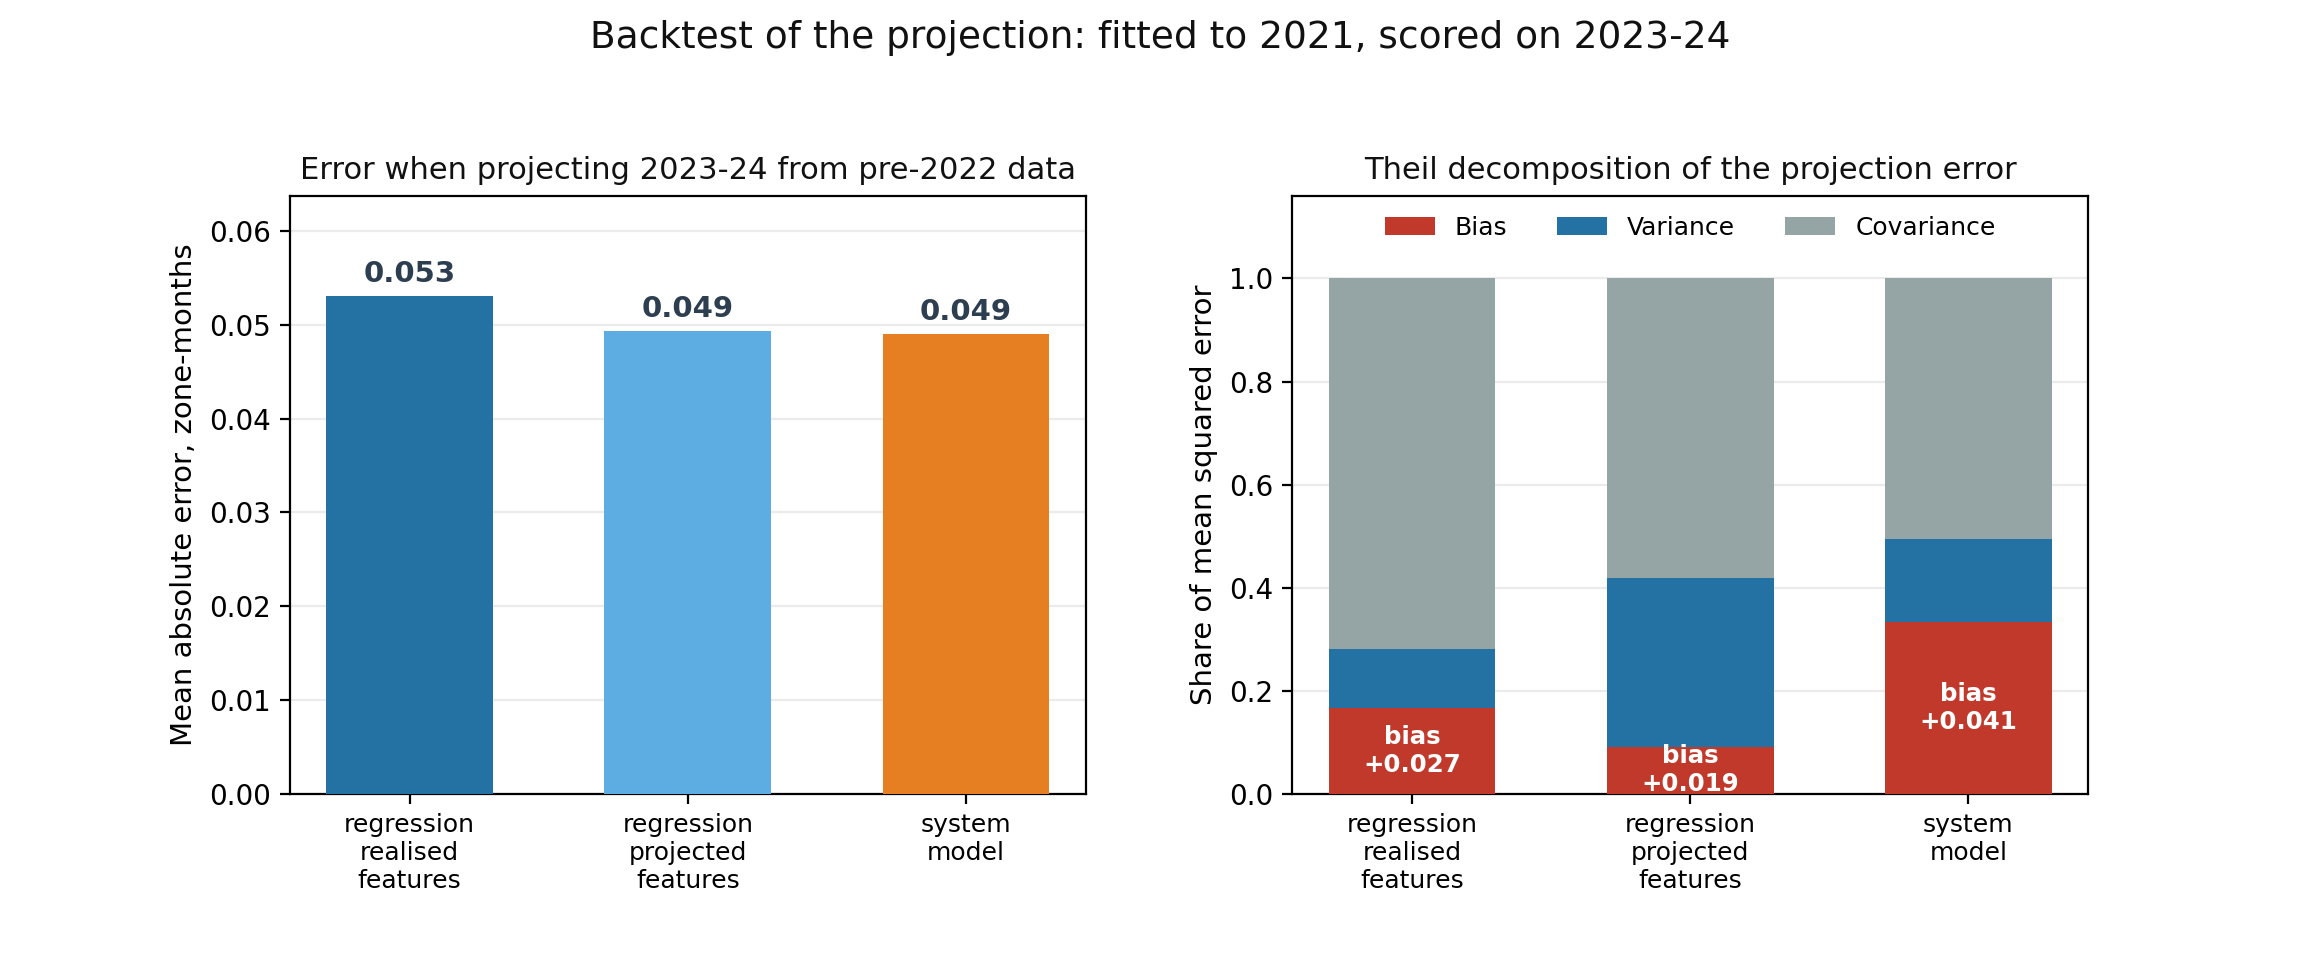
\includegraphics[width=0.92\textwidth]{fig_projection_backtest}
    \caption{Backtesting the projection. Left: error when each approach is
    fitted to 2021 and asked for 2023 and 2024; constructing the input vectors
    costs nothing, and the constructed-input regression matches the system
    model. Right: the Theil partition, where the system model remains the more
    bias-dominated of the two.}
    \label{fig:backtest}
\end{figure}
\FloatBarrier

\subsection{The two projections against external evidence}

Neither model can be scored at 2040, because 2040 has no observations. But the
projections are not therefore unfalsifiable, because the published literature
carries expectations against which both can be placed
(Table~\ref{tab:external}). Running the regression model forward exactly as its
predecessor does, building twelve monthly feature vectors per horizon from the
scenario levels and the farm's own seasonal shape, it returns a Baltic 2040
band of 0.72 to 0.85 with no farm inside the training range. The system model
returns 0.36 to 0.60, centrally 0.47.

Read naively, this favours the regression model. Its band sits inside the
published range and brackets Germany's measured 0.76 almost exactly, while the
system model falls below every benchmark. The reading inverts once the
penetrations at which those benchmarks were measured are attached to them.
Hirth's band is estimated at a 30\,\% share and Germany's 0.76 at 35\,\%, both
comfortably inside the regression model's training range. A model that cannot
leave the regime it was fitted on will land among benchmarks drawn from that
same regime whether or not it is right about 2040, so the agreement is not
corroboration. It is the constant response of Section~\ref{sec:gap_decomposition} producing
a plausible number.

The benchmark that discriminates is the one measured in a market that is
already saturated. Aurora's French offshore holds near 0.94 to 2060, which is
an under-built market and the analogue of the Baltic today rather than the
Baltic of 2040; its French solar, heavily built out, falls to about 0.59 and
stays there \cite{Aurora2025_France}. That is the closest available analogue to
what the Baltic becomes, and it lies inside the system model's raw range and
above the regression model's band. The comparison is developed further in
Section~\ref{sec:disc_literature}.

The decisive quantity, however, is neither estimate. Between a baseline Baltic
buildout and a high one, the regression model's answer moves by 0.008 while the
system model's moves by 0.428. A projection that barely changes between two
different futures is not a forecast of the buildout, however reasonable its
value looks beside the literature. This is what the constant response means in practice, and it is the reason
the external evidence confirms the allocation of roles rather than
establishing it.

\begin{table}[!htb]
\centering\small
\caption{The two projections for the Baltic in 2040, against published
benchmarks. The penetration column is what makes the comparison work: every
benchmark below the rule was measured inside the regression model's training
range, and only the last was measured in a saturated market.}
\label{tab:external}
\begin{tabular}{l c l}
\toprule
\textbf{Source} & \textbf{Capture value} & \textbf{Measured at} \\
\midrule
Regression model, 2040 Baltic & 0.72--0.85 & no farm inside training range \\
System model, 2040 Baltic & 0.36--0.60 (central 0.47) & projected buildout \\
\midrule
Hirth \cite{Hirth2013} & 0.5--0.8 & 30\,\% share \\
Germany \cite{Stiewe2025, Ember2025} & 0.76 & 35\,\% share \\
Jacquet, worst North Sea case \cite{Jacquet2024} & $\approx 0.6$ & North Sea buildout \\
Aurora, French offshore \cite{Aurora2025_France} & $\approx 0.94$ & under-built market \\
\midrule
Aurora, French solar \cite{Aurora2025_France} & $\approx 0.59$ & \textbf{saturated market} \\
\bottomrule
\end{tabular}
\end{table}
\FloatBarrier



\section{The Analytical Equation}\label{app:analytical}

Section~\ref{sec:one_equation} states the conclusion of the per-basin
analytical fit. This appendix carries it in full.

\subsection{One equation, two basins}

SHAP names the influential features; the analytical equation describes the
mechanism's shape in closed form. Refit per basin, the same equation fits both
seas and answers the second research question in its sharpest form: the
pattern-penalty exponent is 0.74 in
the Baltic against 0.37 in the North Sea, steeper in 99 of 100 farm-block
bootstraps (Figure~\ref{fig:constants}). The absolute fit is low by design,
fitted for interpretable shape rather than prediction, so the load-bearing
result is the bootstrap-stable gap. Since the exponent trades off against the
penalty's scale, the fair summary is the implied slope of capture value against
penetration at common conditions: about 1.6 times the North Sea's today and 1.9
times at the dominance a buildout creates. On a fifteen-farm panel that is
directional rather than definitive, but it is consistent with the system model's
moderate-2030, severe-2040 trajectory
(Section~\ref{sec:projection_results}).


\section{Regression Validation and Earlier-Horizon Maps}\label{app:reg_tables}

Supporting Sections~\ref{sec:trust} and~\ref{sec:maps}; the numbers are quoted
in the body.

\begin{table}[!htb]
\centering
\small
\caption{The five algorithm families, out-of-sample $R^2$ on the bidding-zone panel, untuned. Random K-fold withholds farm-months; leave-farm-out withholds whole farms, so it scores entirely unseen sites, where the polynomial's squared and cross terms explode.}
\label{tab:algorithms}
\begin{tabular}{l c c}
\toprule
\textbf{Algorithm} & \textbf{Random K-fold} & \textbf{Leave-farm-out (strict)} \\
\midrule
Gradient boosting (XGBoost) & 0.752 & \textbf{0.686} \\
Random forest & 0.682 & 0.636 \\
Support-vector regression & 0.583 & 0.497 \\
Linear (OLS) & 0.330 & 0.270 \\
Polynomial (degree~2) & 0.437 & $-19.9$ \\
\bottomrule
\end{tabular}
\end{table}

\begin{table}[!htb]
\centering
\small
\caption[Out-of-sample $R^2$ of the gradient-boosting model per scheme]{Out-of-sample $R^2$ of the untuned gradient-boosting model under each
scheme, at country versus bidding-zone resolution. Both K-fold rows are scored
out-of-fold and differ only in what they withhold: random farm-months (leaky,
for comparability with Jacquet's untuned 0.82 \cite{Jacquet2024}) versus whole farms
(strict).}
\label{tab:regression_metrics}
\begin{tabular}{l c c}
\toprule
\textbf{Validation scheme} & \textbf{Country features} & \textbf{Zone features} \\
\midrule
Random K-fold (comparability) & 0.733 & 0.752 \\
Leave-farm-out (headline) & 0.598 & \textbf{0.686} \\
Leave-farm-out, excluding 2022 & 0.607 & 0.692 \\
North Sea $\rightarrow$ Baltic transfer & 0.360 & 0.379 \\
Time split (train $\leq$2022, test 2023--24) & $-0.093$ & $-0.032$ \\
\bottomrule
\end{tabular}
\end{table}

\begin{figure}[!htb]
    \centering
    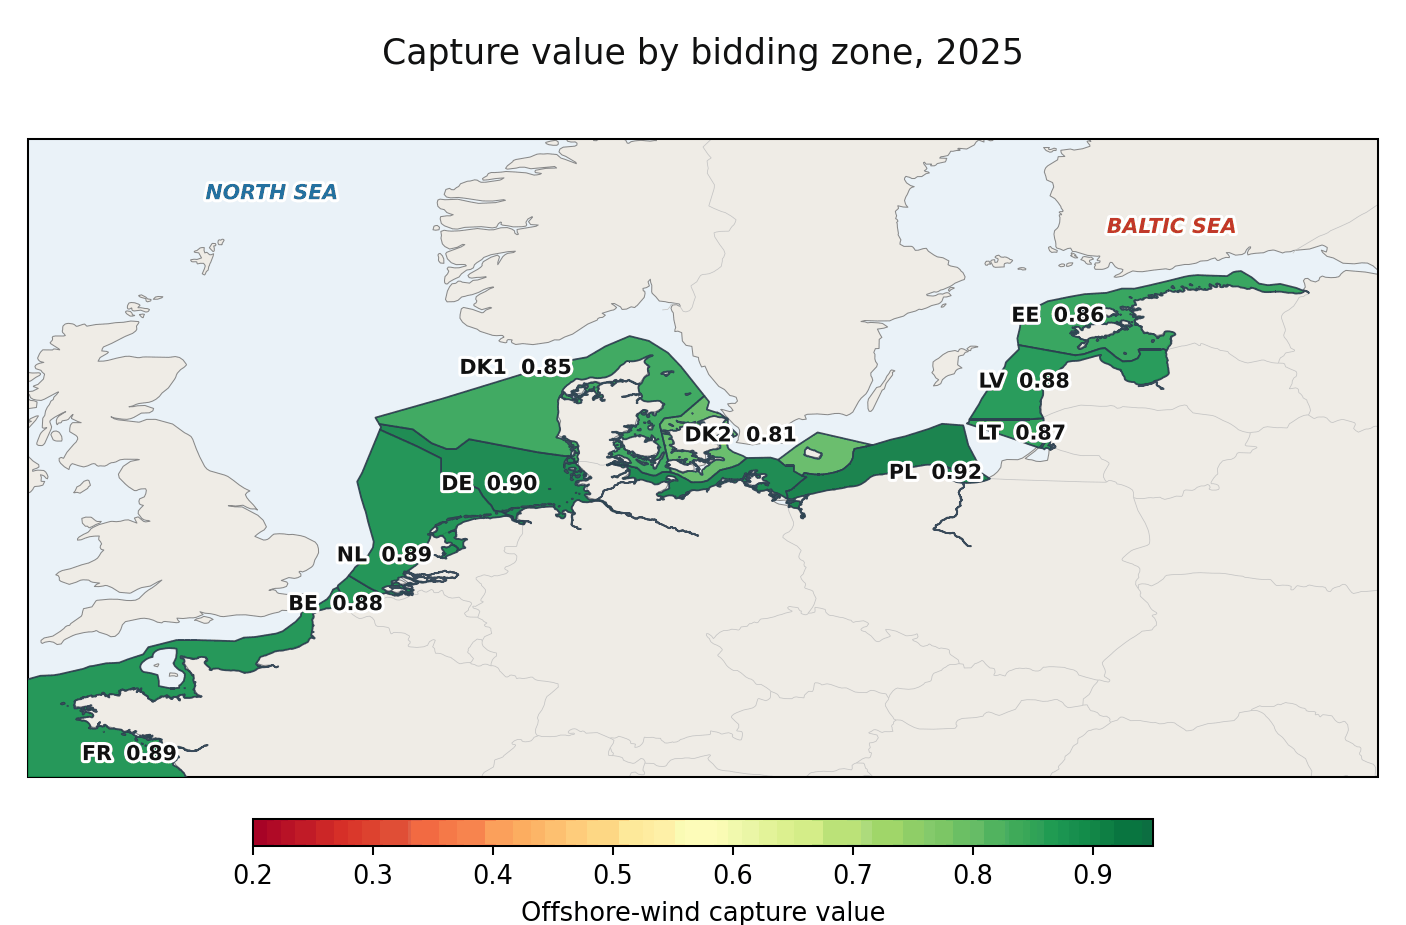
\includegraphics[width=0.80\textwidth]{fig_heatmap_2025}
    \caption{Offshore capture value across both shelves, 2025. Capture value is high and nearly uniform across both shelves: the under-built
    Baltic sits level with the North Sea, and
    the theoretical Baltic premium is not visible.}
    \label{fig:heatmap_2025}
\end{figure}

\begin{figure}[!htb]
    \centering
    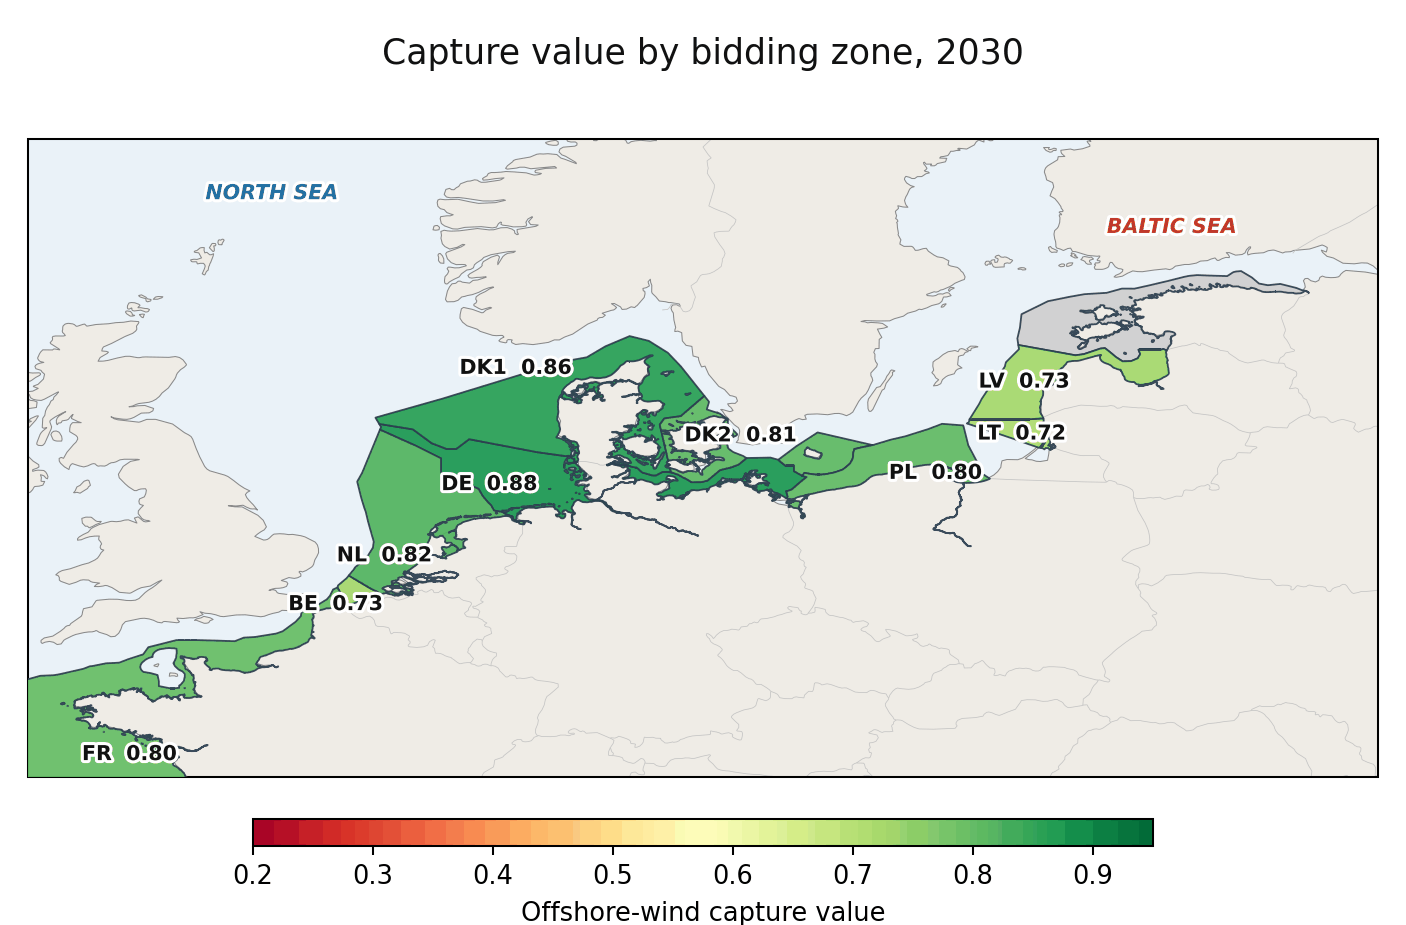
\includegraphics[width=0.80\textwidth]{fig_heatmap_2030}
    \caption{The same field in 2030. The first tranche of the buildout is in place. Values have fallen slightly
    and remain high in both basins, with the Baltic beginning to fall further
    as its own correlated output crowds its price.}
    \label{fig:heatmap_2030}
\end{figure}
\section{Model Comparison Against Observed Prices: Full Detail}\label{app:triangle}

The per-zone-year detail behind Sections~\ref{sec:trust}
and~\ref{sec:why_differ}; the aggregates are quoted in the body.

\begin{table}[!htb]
\centering\small
\caption{The three-way comparison in numbers: observed capture value against
each model's estimate, with signed errors, for all fifteen zone-years. The
regression column is out of fold, from a model that never trained on the
zone's farms.}
\label{tab:triangle}
\begin{tabular}{l l c c c r r}
\toprule
\textbf{Zone} & \textbf{Year} & \textbf{Observed} & \textbf{Regression} &
\textbf{System model} & \textbf{Reg.\ error} & \textbf{Sys.\ error} \\
\midrule
DE  & 2019 & 0.923 & 0.948 & 0.984 & $+0.025$ & $+0.061$ \\
NL  & 2019 & 0.977 & 0.967 & 0.986 & $-0.010$ & $+0.009$ \\
BE  & 2019 & 0.919 & 0.925 & 0.983 & $+0.006$ & $+0.064$ \\
DK1 & 2019 & 0.924 & 0.929 & 0.986 & $+0.005$ & $+0.062$ \\
DK2 & 2019 & 0.933 & 0.936 & 0.987 & $+0.003$ & $+0.054$ \\
\addlinespace
DE  & 2023 & 0.909 & 0.913 & 0.908 & $+0.004$ & $-0.001$ \\
NL  & 2023 & 0.881 & 0.887 & 0.883 & $+0.006$ & $+0.002$ \\
BE  & 2023 & 0.869 & 0.879 & 0.896 & $+0.010$ & $+0.027$ \\
DK1 & 2023 & 0.854 & 0.861 & 0.917 & $+0.007$ & $+0.063$ \\
DK2 & 2023 & 0.784 & 0.798 & 0.927 & $+0.014$ & $+0.143$ \\
\addlinespace
DE  & 2024 & 0.910 & 0.896 & 0.941 & $-0.014$ & $+0.031$ \\
NL  & 2024 & 0.900 & 0.878 & 0.919 & $-0.022$ & $+0.019$ \\
BE  & 2024 & 0.893 & 0.869 & 0.928 & $-0.024$ & $+0.035$ \\
DK1 & 2024 & 0.843 & 0.833 & 0.947 & $-0.010$ & $+0.104$ \\
DK2 & 2024 & 0.808 & 0.802 & 0.949 & $-0.006$ & $+0.141$ \\
\bottomrule
\end{tabular}
\end{table}

\begin{figure}[!htb]
    \centering
    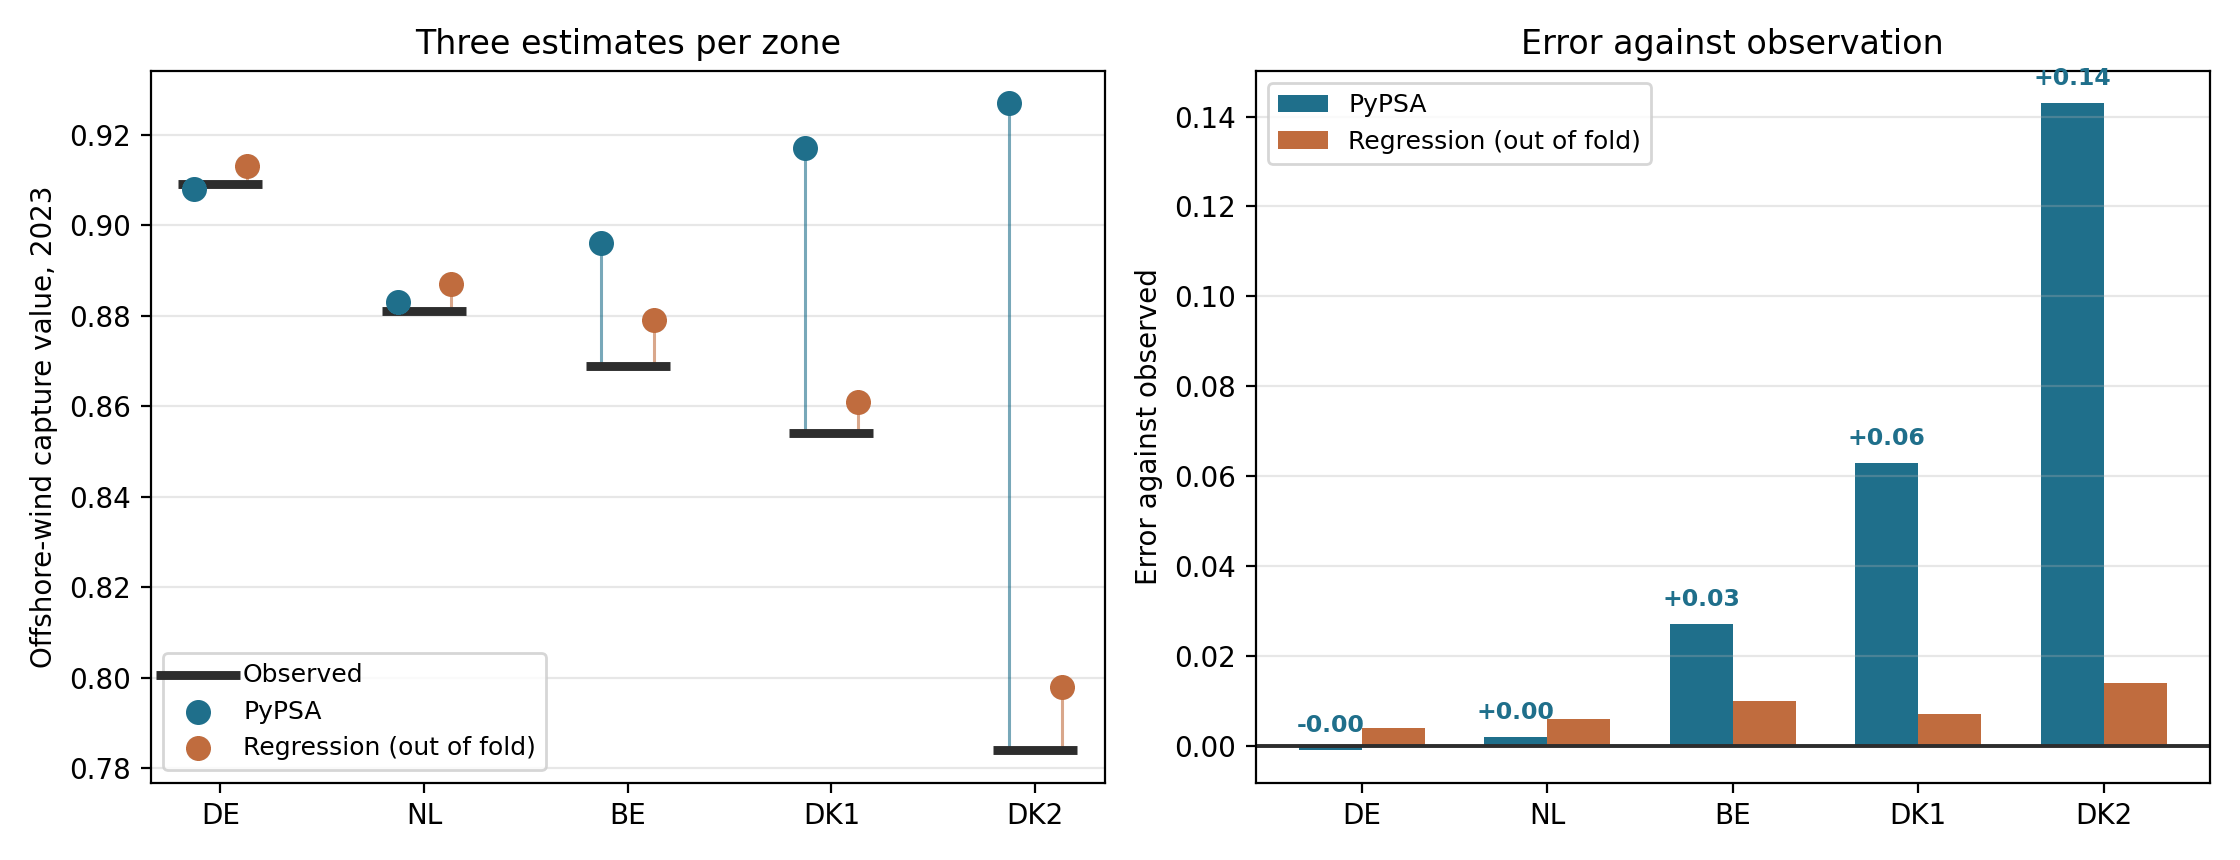
\includegraphics[width=0.95\textwidth]{fig_validation_triangle_2023}
    \caption{The three-way comparison, 2023. Left: the three estimates per zone, observed as the black tick. Right: each model's error. The regression stays within about 0.01 everywhere; the system model's error grows with congestion.}
    \label{fig:triangle}
\end{figure}

\begin{table}[!htb]
\centering\small
\caption{The gap between the two models, decomposed. Channels sum exactly to the
total in every row. Positive means the channel moves the system model's capture
value above the regression model's. Weights are offshore energy.}
\label{tab:gap_channels}
\begin{tabular}{l c c c c c c c}
\toprule
& \textbf{Regression} & \textbf{System} & \textbf{Total} &
\textbf{Constr.} & \textbf{Gener-} & \textbf{Zero} & \textbf{Price} \\
\textbf{Zone} & \textbf{model} & \textbf{model} & \textbf{gap} &
\textbf{residual} & \textbf{ation} & \textbf{floor} & \textbf{shape} \\
\midrule
DE  & 0.913 & 0.888 & $-0.025$ & $-0.014$ & $-0.012$ & $+0.002$ & $+0.002$ \\
NL  & 0.887 & 0.877 & $-0.010$ & $\phantom{-}0.000$ & $+0.009$ & $+0.005$ & $-0.023$ \\
BE  & 0.879 & 0.880 & $+0.001$ & $+0.002$ & $+0.020$ & $+0.002$ & $-0.025$ \\
DK1 & 0.861 & 0.917 & $+0.056$ & $\phantom{-}0.000$ & $+0.007$ & $+0.002$ & $-0.003$ \\
\midrule
Weighted mean & 0.890 & 0.885 & $-0.005$ & $-0.003$ & $+0.004$ & $+0.003$ & $-0.014$ \\
\bottomrule
\end{tabular}
\\[4pt]
{\footnotesize The network-representation channel is $-0.003$ (DE), $-0.001$
(NL), $+0.003$ (BE), $+0.050$ (DK1) and $+0.004$ weighted; it is reported
separately because it is the one channel already corrected in
Section~\ref{sec:division}.}
\end{table}

\begin{figure}[!htb]
    \centering
    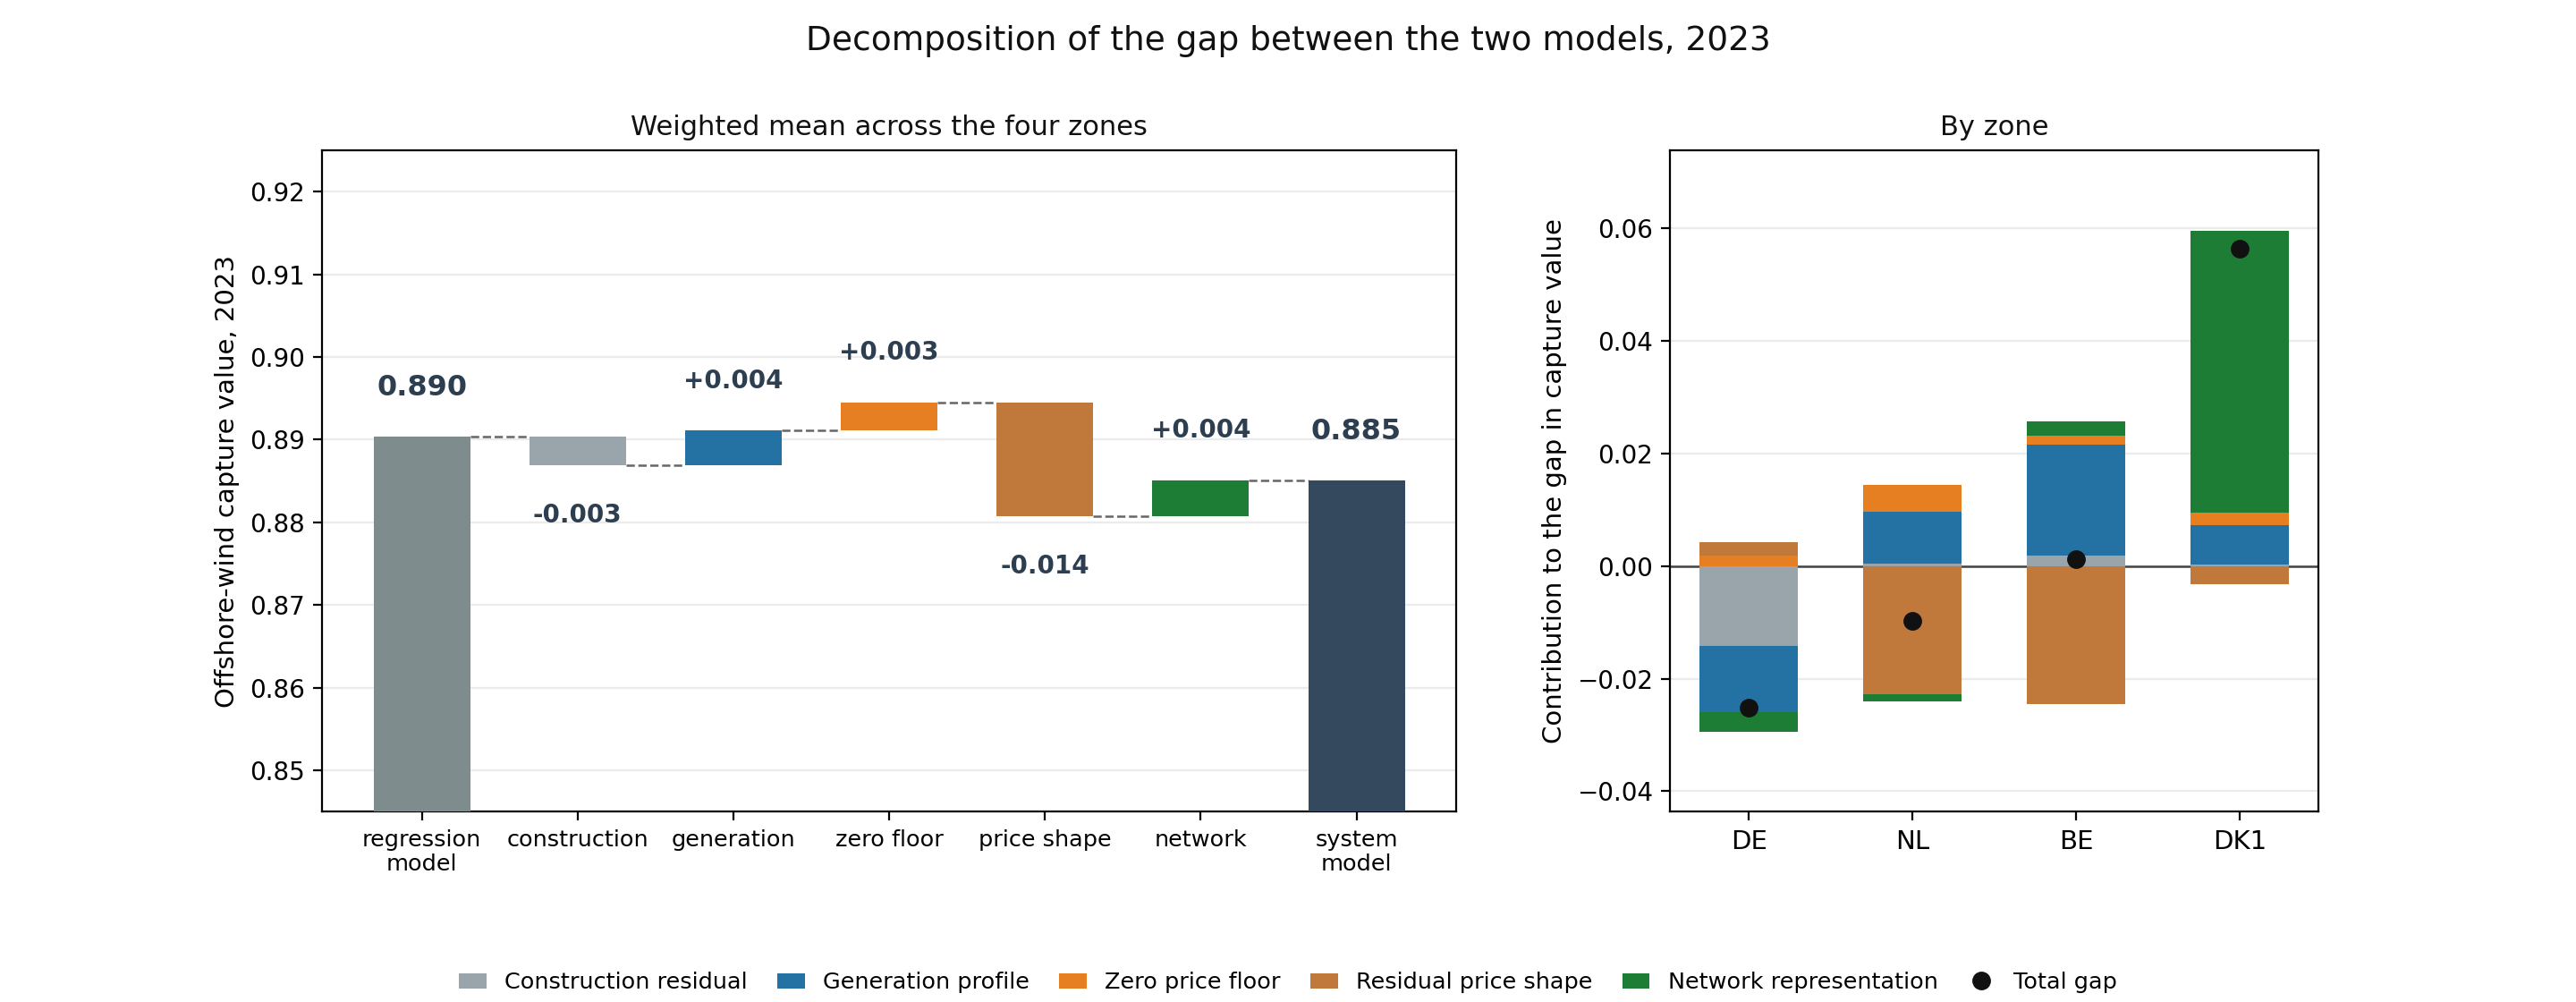
\includegraphics[width=0.98\textwidth]{fig_model_gap_decomposition}
    \caption{Decomposition of the gap between the two models, 2023. Left: the bridge from the regression model's estimate to the system model's, energy-weighted across the four zones. Right: the same channels by zone. Positive values move the system model above the regression model.}
    \label{fig:gap_decomp}
\end{figure}

\begin{figure}[!htb]
    \centering
    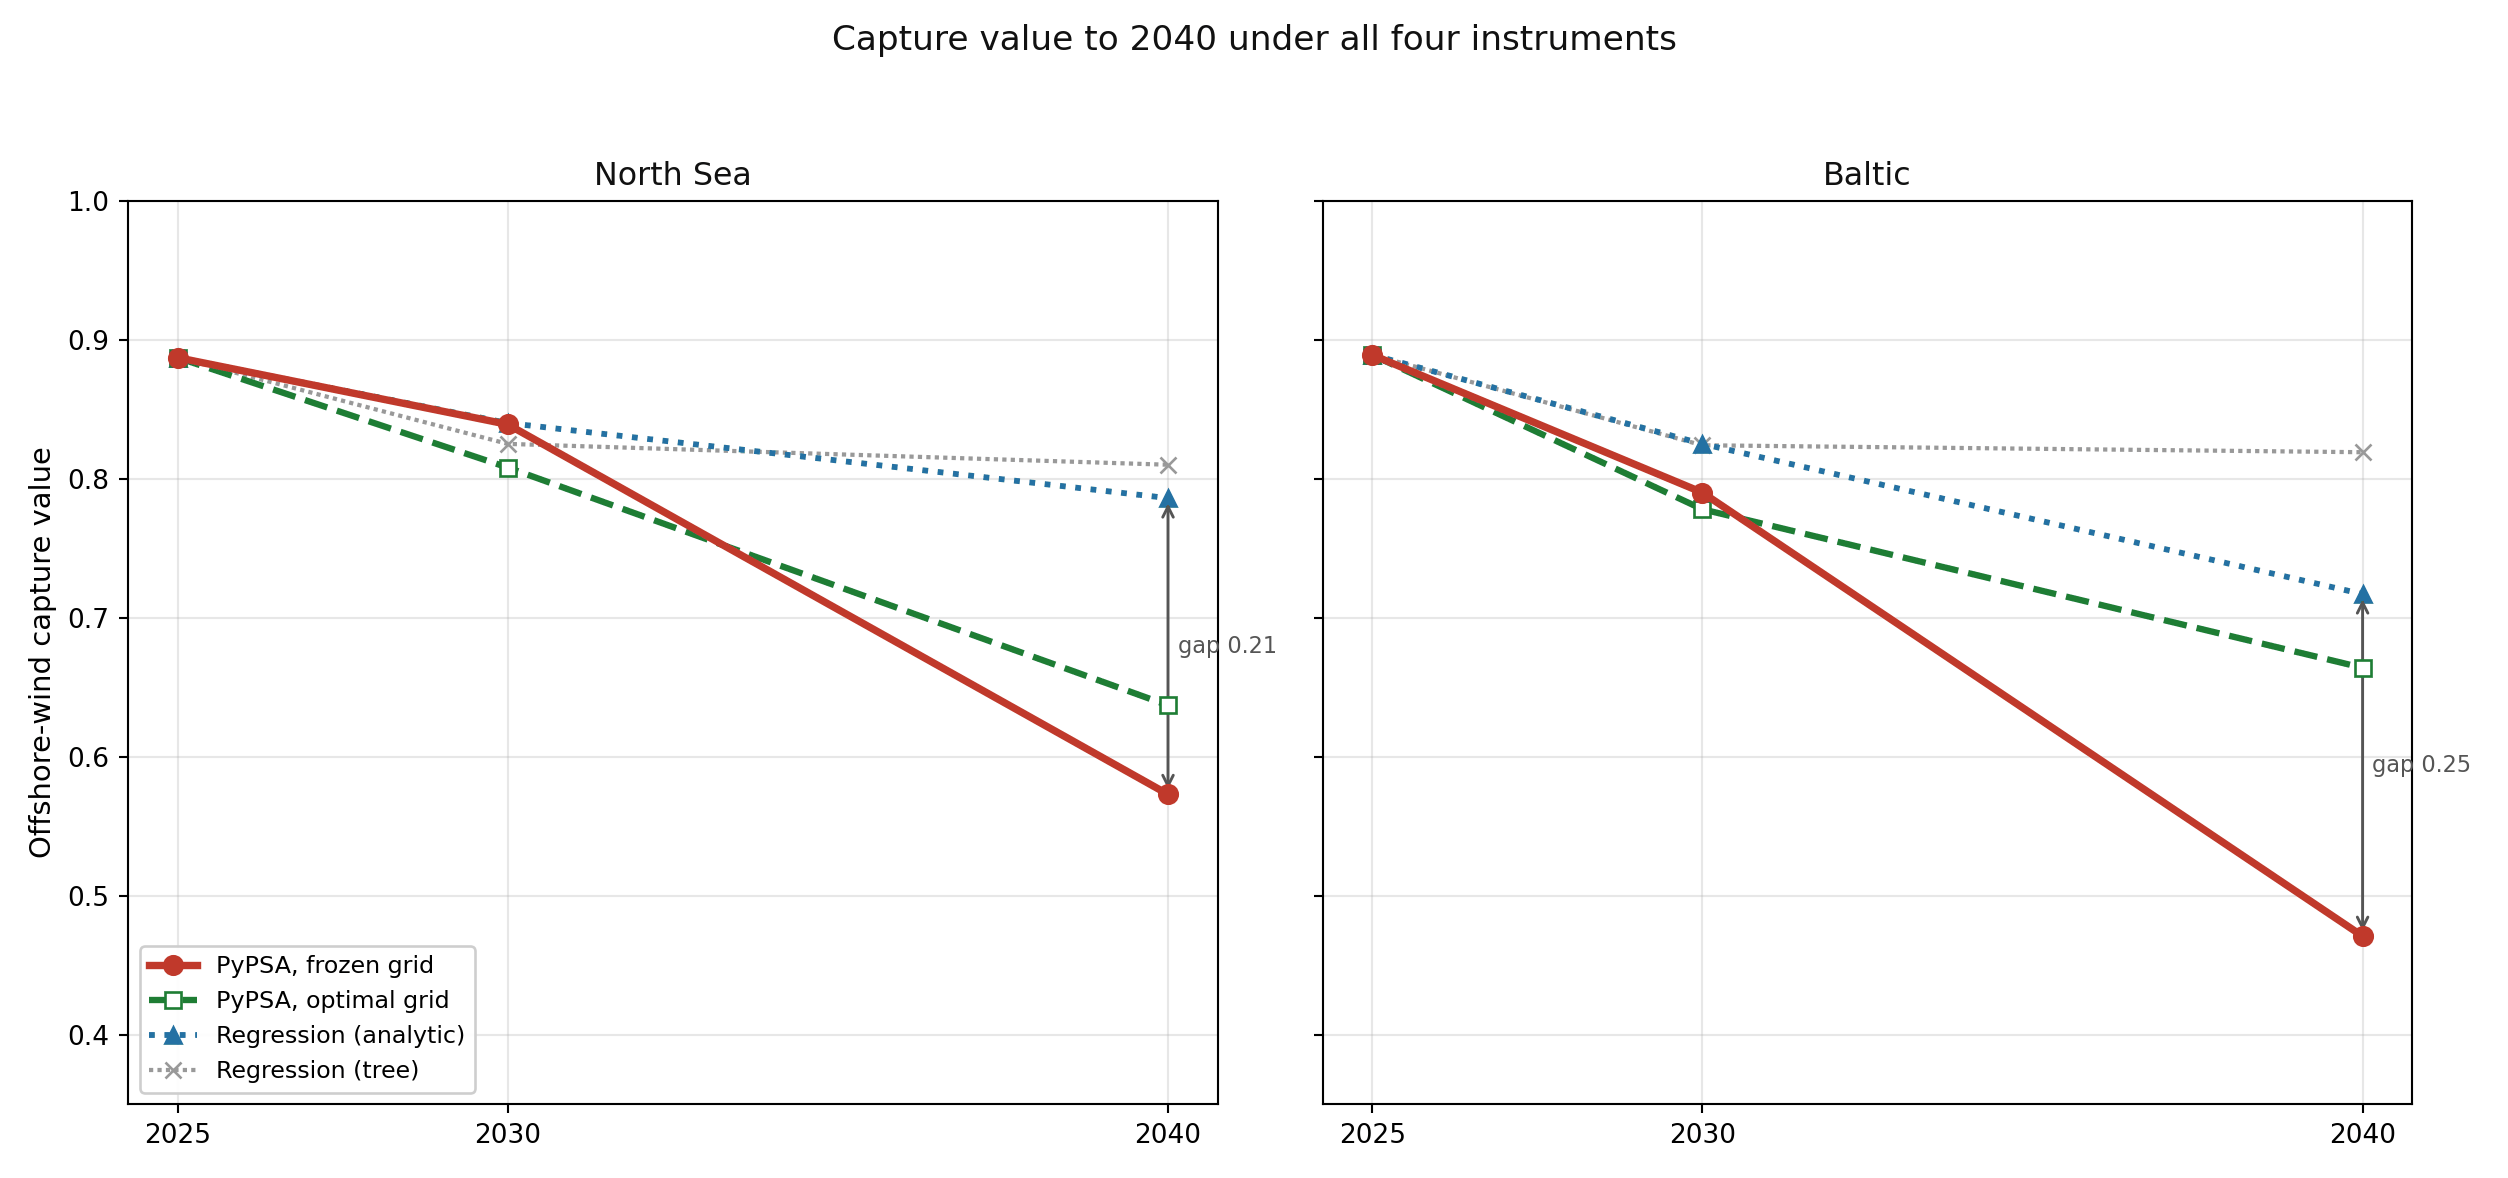
\includegraphics[width=0.88\textwidth]{fig_capture_value_evolution}
    \caption{Every model on one axis, 2025 to 2040. The models
    agree to 2030; at 2040 the regression model returns a constant, the analytical form falls
    gently, and the system model finds the collapse the others cannot.}
    \label{fig:cv_evolution}
\end{figure}

\begin{figure}[!htb]
    \centering
    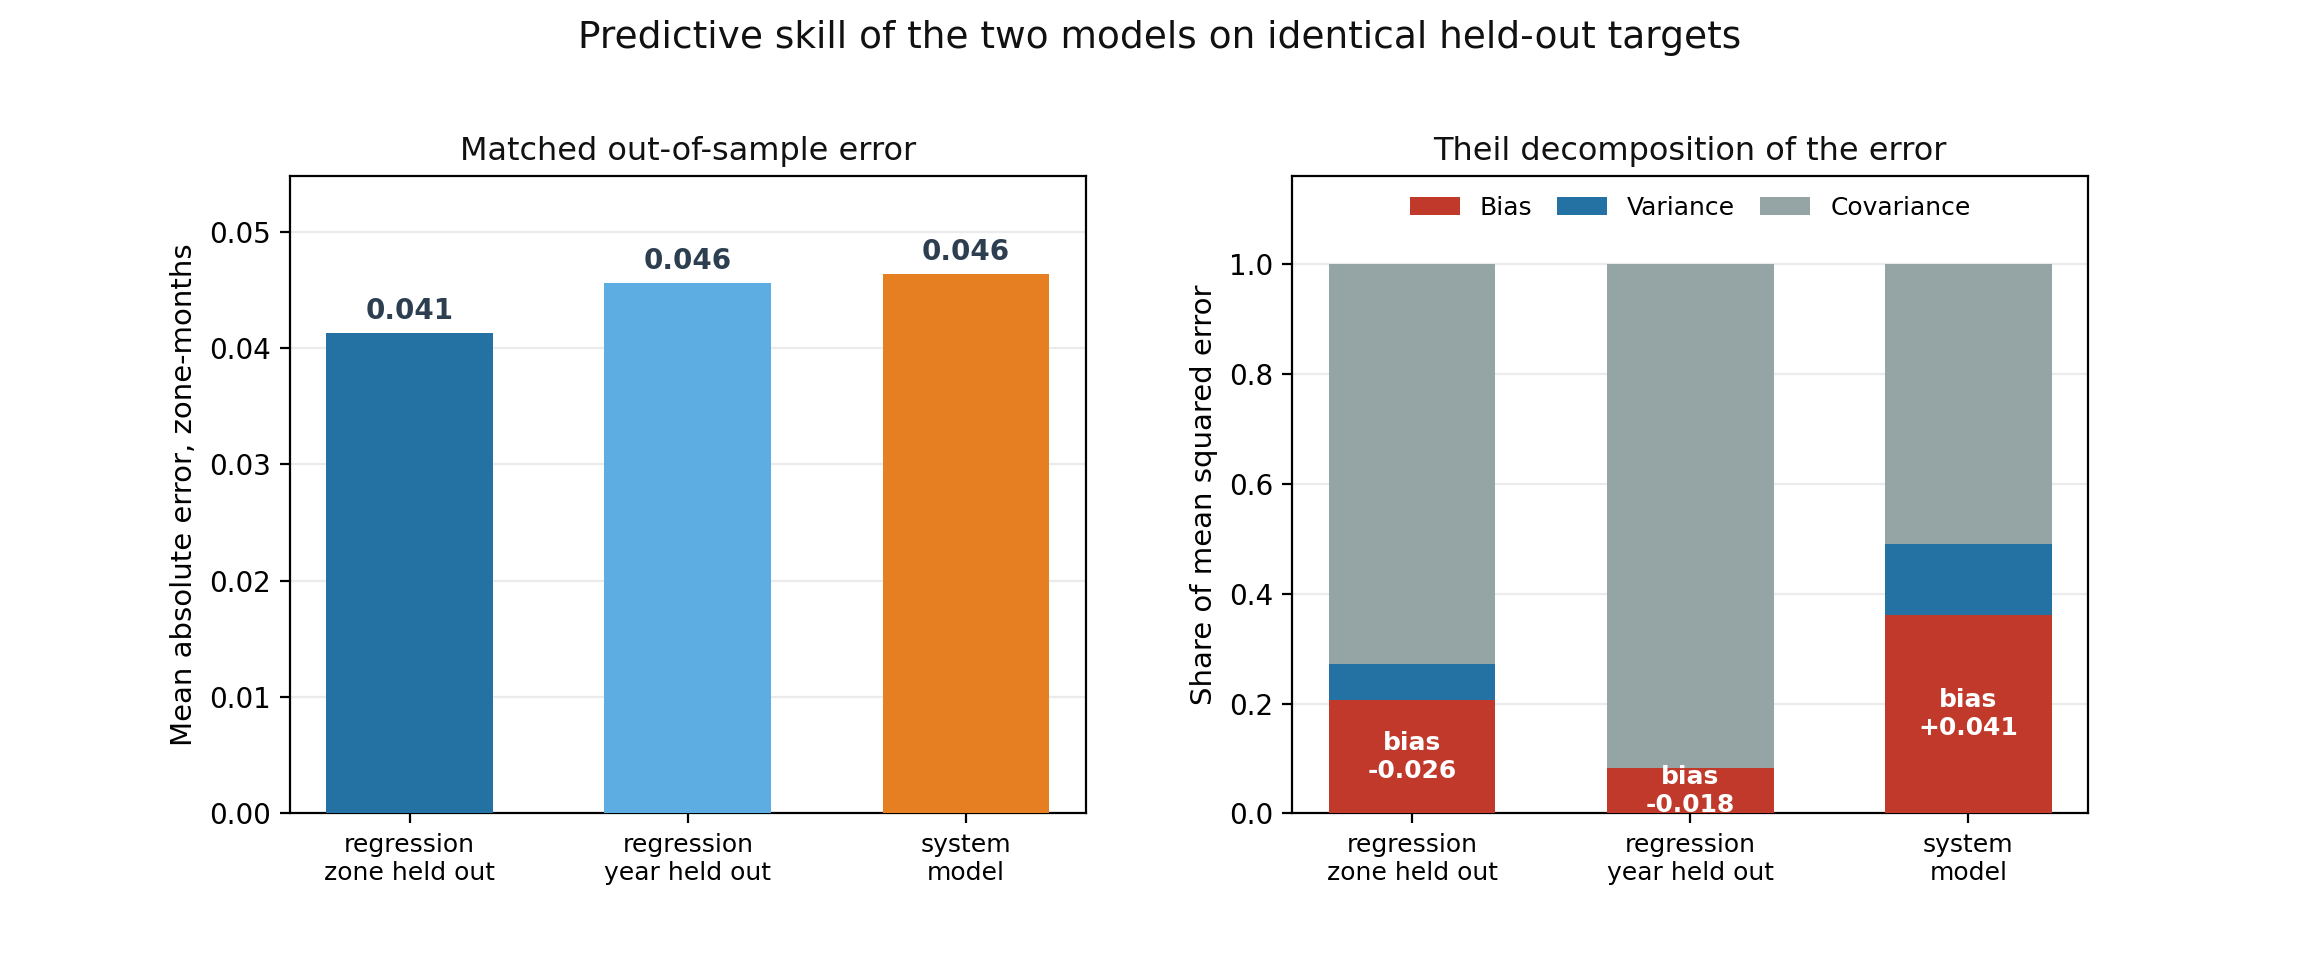
\includegraphics[width=0.92\textwidth]{fig_model_skill}
    \caption{Predictive skill on identical held-out targets. Left: average error,
    indistinguishable across the three schemes. Right: the decomposition of
    squared error into a systematic component, a component from failing to match
    the spread of the observations, and a component from imperfect correlation.
    The system model's error is a third systematic; the regression model's is
    almost entirely imperfect correlation.}
    \label{fig:skill}
\end{figure}

\section{Reproducibility}\label{app:repro}

The entire project is a numbered pipeline: scripts 1.01 to 1.20 (system model), 2.01 to 2.13 (regression model), and 3.01 (the comparison with observation), each reading its predecessors' outputs from disk and writing
its own next to them. A single refresh chain re-solves everything from the
prepared networks to the final tables in about three hours on a workstation
(Apple Silicon, Gurobi academic licence); individual scenario solves take
about 90 seconds at solver parity. Every headline number regenerates from
public data: ENTSO-E Transparency, ERA5 via Open-Meteo and atlite, TYNDP
2024 workbooks, and open cost data. Configuration files pin every assumption
of Appendix~\ref{app:assumptions}; staleness guards (input modification
times recorded next to fitted outputs) make outdated results detectable. A
line-by-line audit log of the one major repair cycle, with before and after
values, is kept in the project repository.

\begin{table}[!htb]
\centering
\small
\caption{Inventory of system-model runs. All solves use the identical model version, solver configuration, and
corrections of this chapter; only the
stated dimension varies.}
\label{tab:runs}
\begin{tabular}{l c p{7.2cm}}
\toprule
\textbf{Run set} & \textbf{Solves} & \textbf{Purpose} \\
\midrule
Historical baselines & 3 & 2019, 2023, and 2024 calibration years \\
Canonical scenarios & 6 & 2030/2040, central and high Baltic buildouts, two
2040 demand pathways \\
Gas-price grid & 15 & three buildouts $\times$ five gas prices, 15 to
120~\euro/MWh \\
Grid bracket & 6 & the six scenarios with optimisable transmission \\
Surrogate training & 55 & 50 Latin-hypercube points plus 5 scenario anchors,
three-hourly, harvested alongside the 21 full-hourly solves above \\
Resolution check & 2 & two design points re-solved at full resolution \\
\bottomrule
\end{tabular}
\end{table}
Table~\ref{tab:versions} pins the software environment behind every solve
and fit.

\begin{table}[!htb]
\centering\small
\caption{The software environment. All versions are those used for the
reported runs; the regression stack is pinned because untuned library defaults
are version-dependent.}
\label{tab:versions}
\begin{tabular}{l l l l}
\toprule
Python & 3.13 & PyPSA-Eur & v2026.02.0 (commit 23c2fac7) \\
pypsa & 1.2.0 & snakemake & 9.20.0 \\
Gurobi & 13.0.2 (academic) & atlite & 0.6.1 \\
xgboost & 3.2.0 & scikit-learn & 1.8.0 \\
pandas & 2.3.3 & numpy & 2.4.3 \\
\bottomrule
\end{tabular}
\end{table}

% ============================================================================
\section{Spatial Atlas}\label{app:atlas}
% ============================================================================

The main text carries one map per argument. This appendix carries the full
spatial series behind them, so that every field is available at all three
horizons rather than only at the year the argument needed. Each family is built
on the same footing: the high-resolution capacity-factor field of
Section~\ref{sec:cost_field}, water depth and distance from GEBCO, and per-zone
capture values read from the solved networks of Section~\ref{sec:projection}. All
maps share a fixed colour scale within their family so that the three horizons
are directly comparable; a field that changes colour between 2025 and 2040 has changed in value.

\FloatBarrier
\subsection*{F.1 The resource field}

\begin{figure}[!htb]
    \centering
    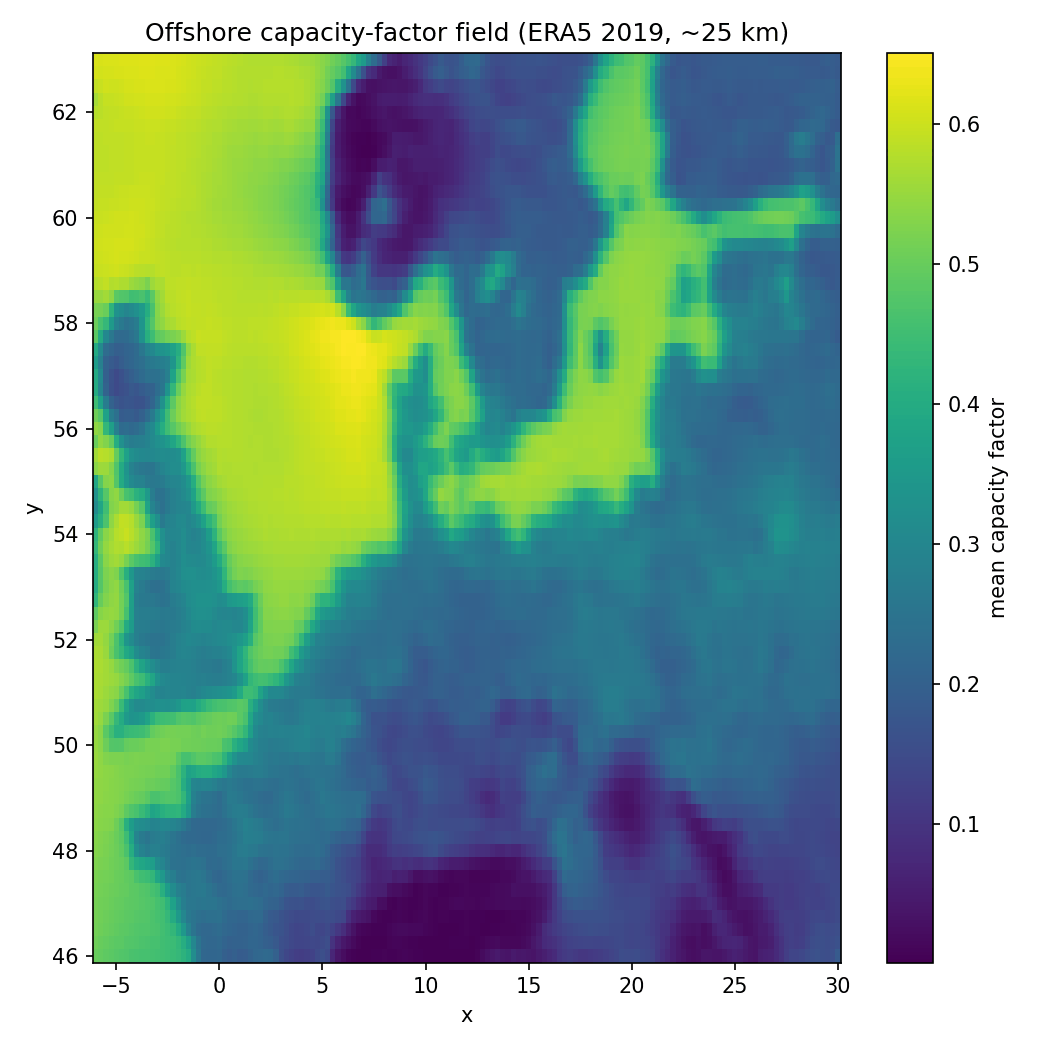
\includegraphics[width=0.80\textwidth]{fig_cf_field_preview}
    \caption{The offshore capacity-factor field across both shelves, built once
    from the Global Wind Atlas at roughly 2~km resolution and used as the common
    resource layer for every economic map that follows. The gradient from the
    open North Sea to the eastern Baltic is the physical starting point for the
    whole comparison, and it is year-independent: the wind field is identical in every year, so the changes in the maps that
    follow come from value and cost.}
    \label{fig:cf_field}
\end{figure}

\FloatBarrier
\subsection*{F.2 Capture value under an optimal grid}

Figures~\ref{fig:heatmap_2025} to~\ref{fig:heatmap_2040} in the main text show
capture value on the frozen grid. The counterfactual matters as much, since the
difference between the two is the congestion component isolated in
Section~\ref{sec:decomposition}. The maps below repeat the sequence with
transmission expanded to the cost optimum.

\begin{figure}[!htb]
    \centering
    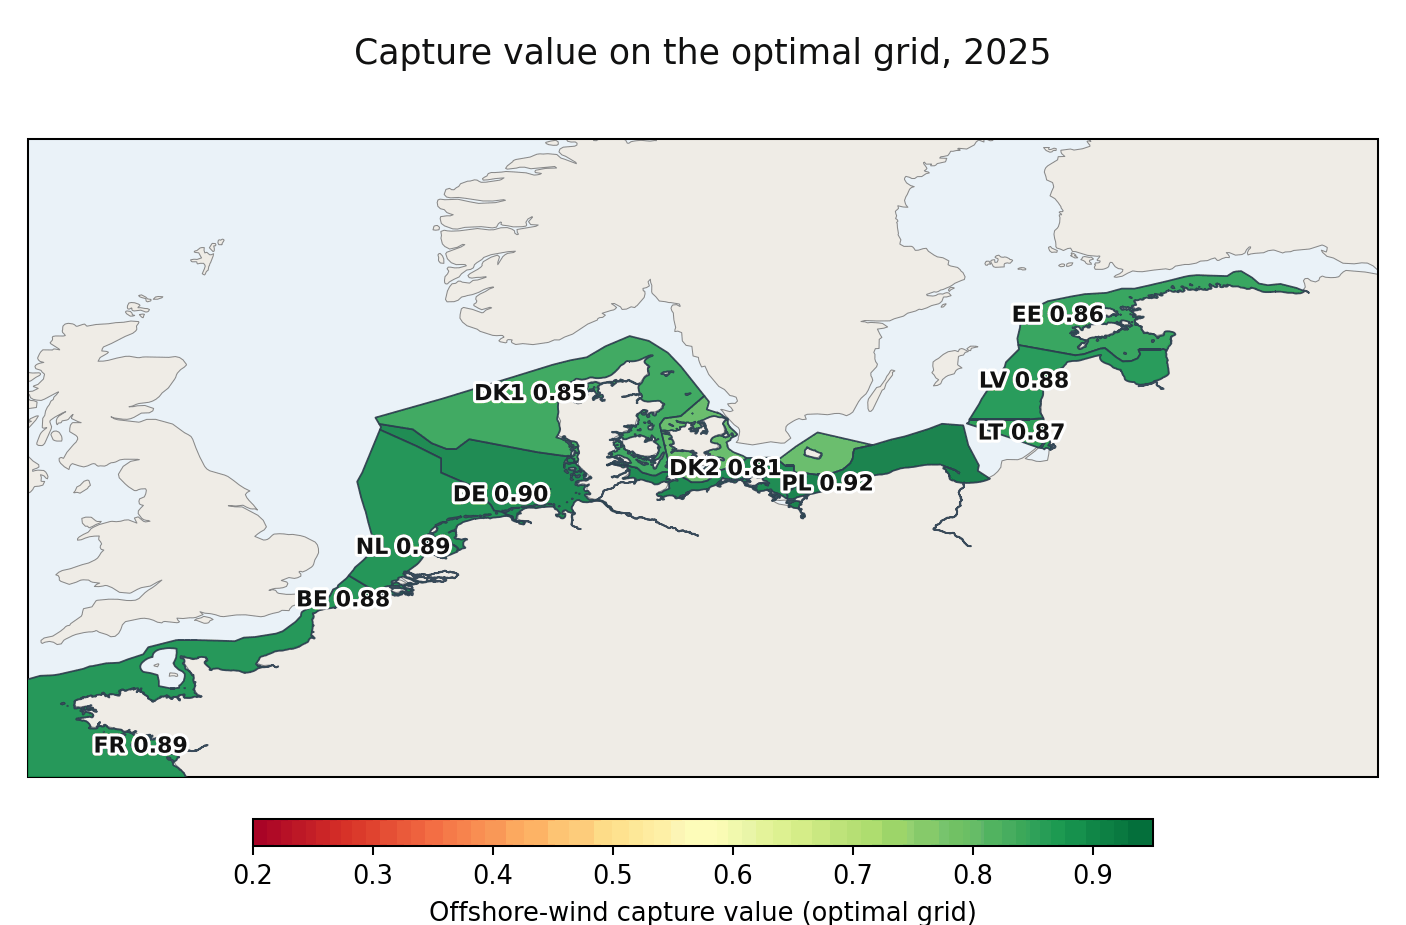
\includegraphics[width=0.72\textwidth]{fig_heatmap_opt_2025}
    \caption{Capture value on the cost-optimal grid, 2025. At today's
    penetration the grid assumption barely matters and the field is
    indistinguishable from the frozen case.}
    \label{fig:heatmap_opt_2025}
\end{figure}

\begin{figure}[!htb]
    \centering
    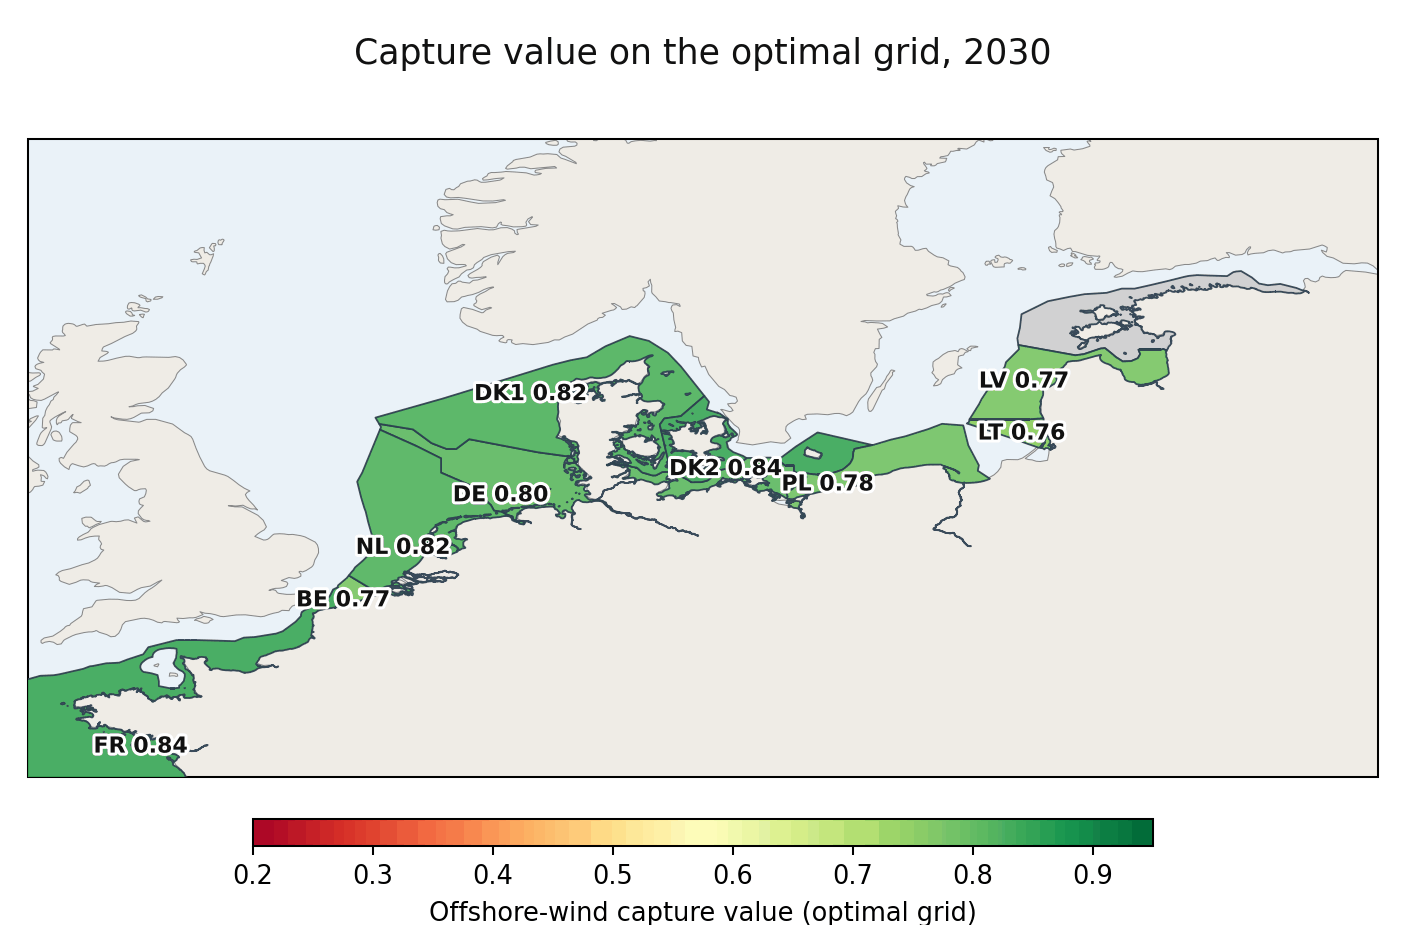
\includegraphics[width=0.72\textwidth]{fig_heatmap_opt_2030}
    \caption{Capture value on the cost-optimal grid, 2030. The bracket is still
    almost nil: congestion has not yet begun to bind.}
    \label{fig:heatmap_opt_2030}
\end{figure}

\begin{figure}[!htb]
    \centering
    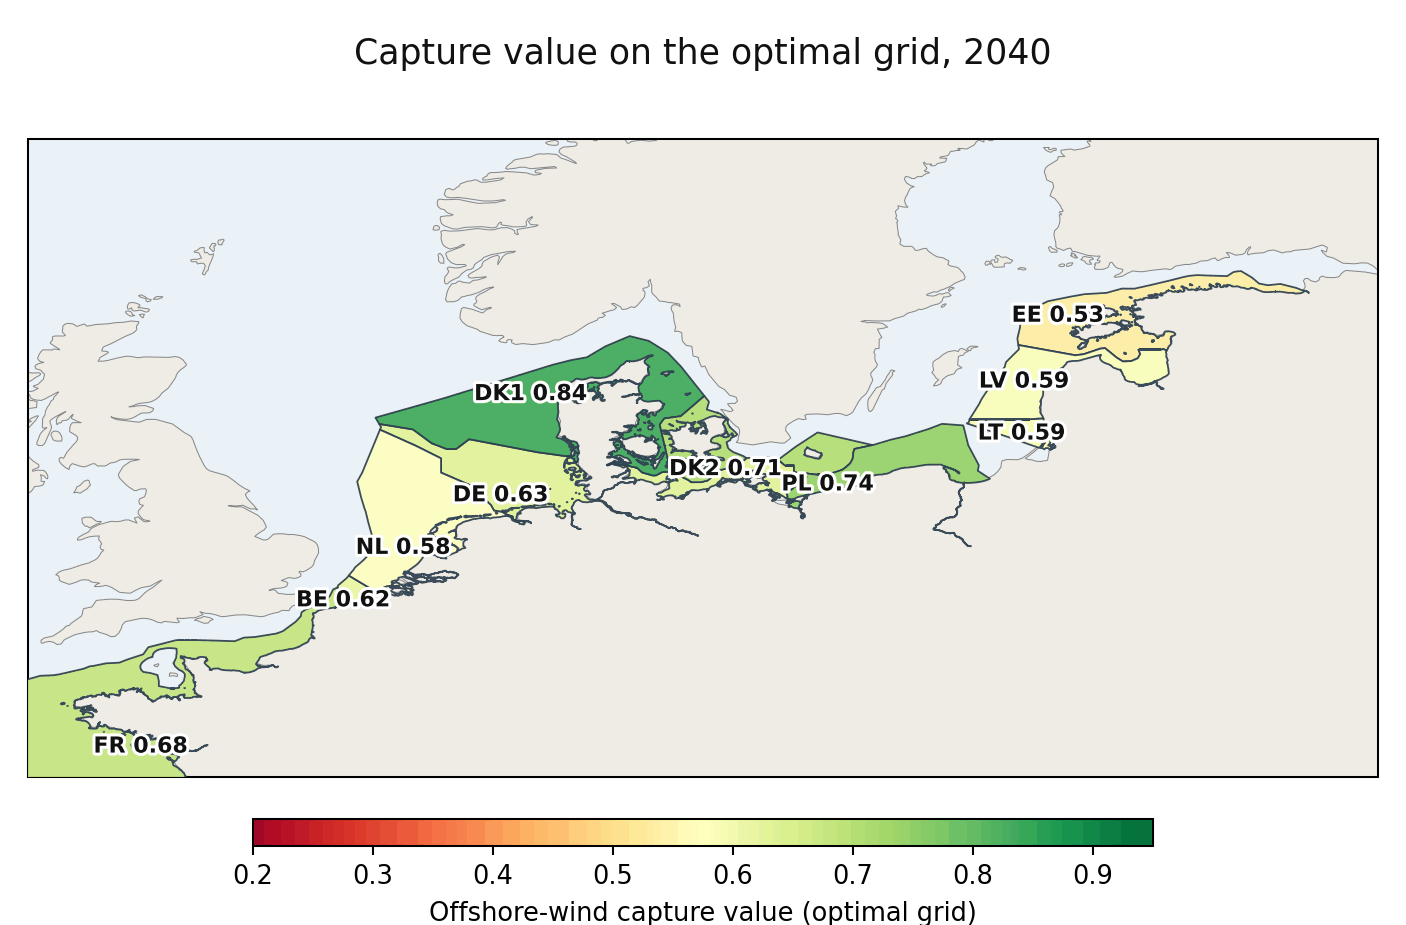
\includegraphics[width=0.72\textwidth]{fig_heatmap_opt_2040}
    \caption{Capture value on the cost-optimal grid, 2040. Compared with
    Figure~\ref{fig:heatmap_2040} the eastern Baltic recovers most, which is the
    spatial expression of the reversal: the zones that lose the most to a frozen
    network are the ones an expanded network restores.}
    \label{fig:heatmap_opt_2040}
\end{figure}

\FloatBarrier
\subsection*{F.3 Levelised cost across the shelf}

The cost field is the standard output of the spatial assessment literature
\cite{Bosch2019} and the baseline against which the value-adjusted metric is
compared. It falls with technology learning and is otherwise governed by depth,
distance and resource.

\begin{figure}[!htb]
    \centering
    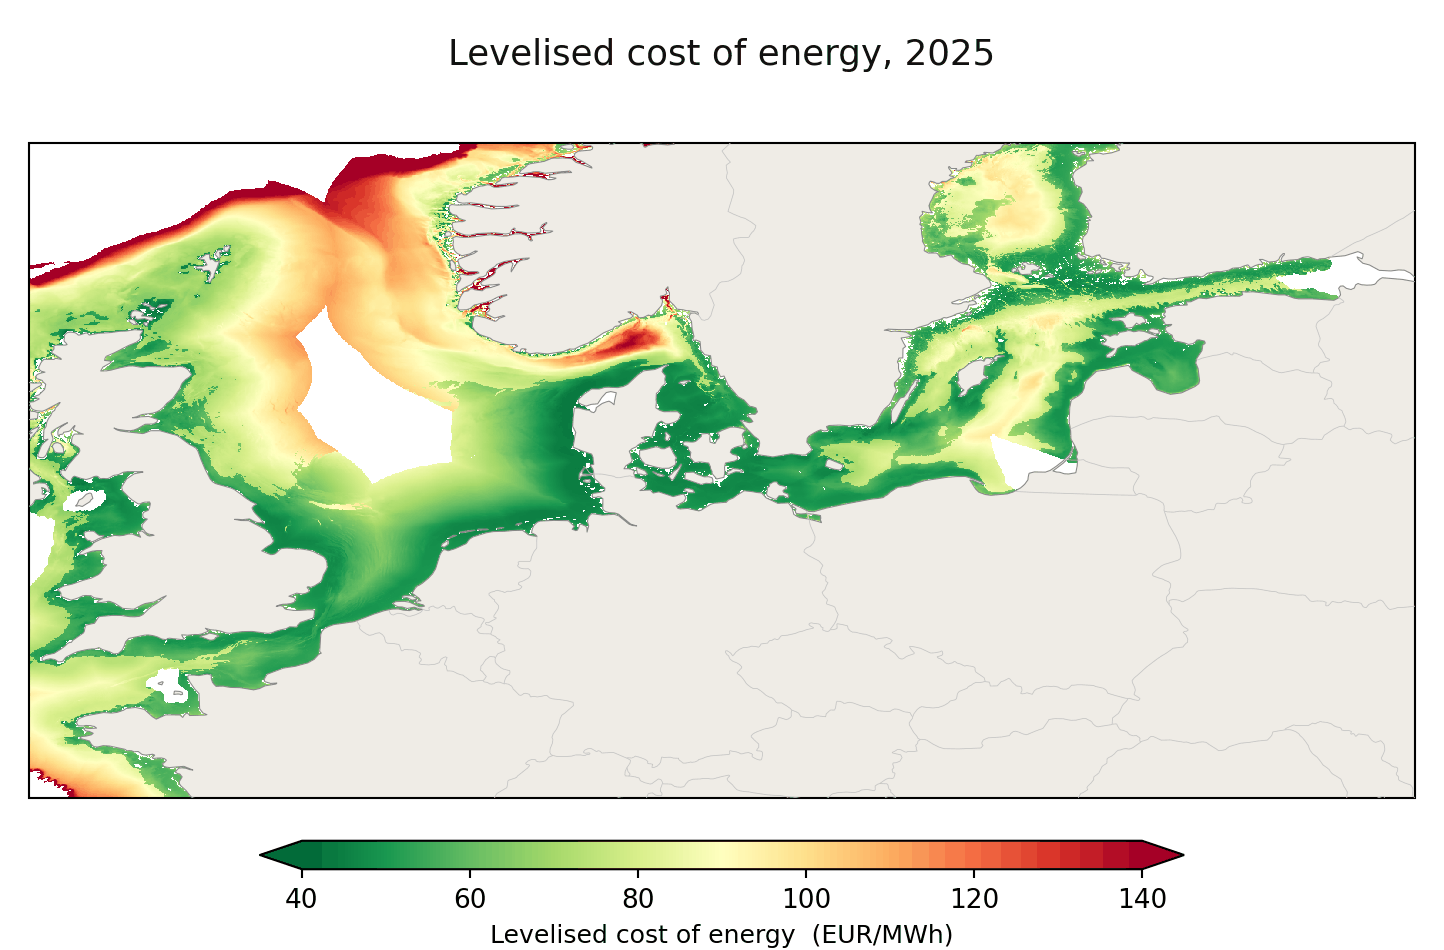
\includegraphics[width=0.72\textwidth]{fig_cost_lcoe_2025}
    \caption{Levelised cost of energy by location, 2025. Cheap sites cluster in
    the shallow southern North Sea and the western Baltic; the deep Norwegian
    trench never clears the floating-foundation premium.}
    \label{fig:cost_2025}
\end{figure}

\begin{figure}[!htb]
    \centering
    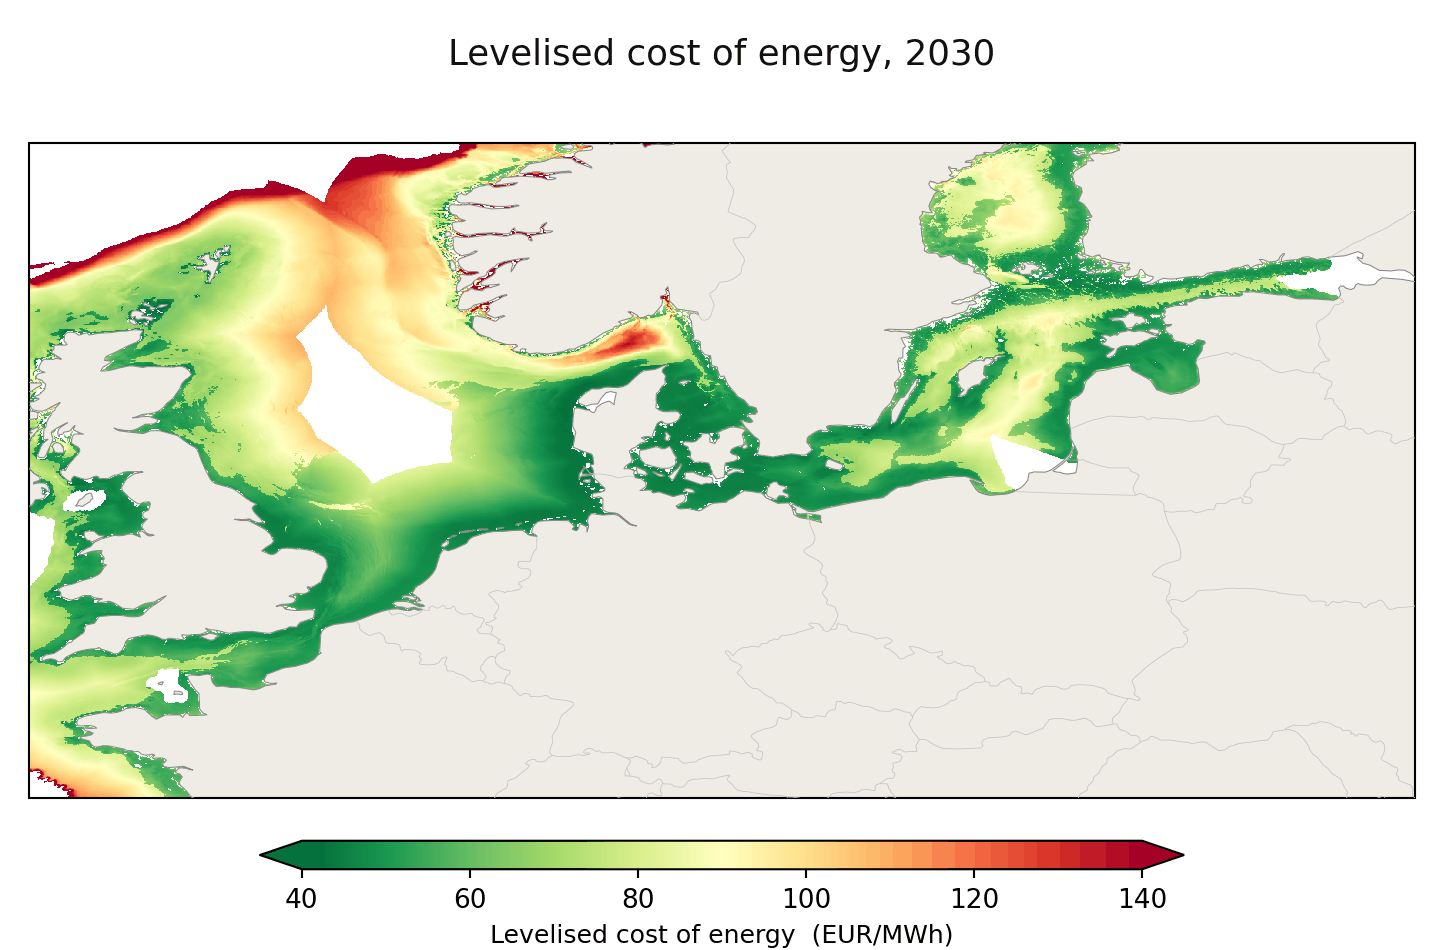
\includegraphics[width=0.72\textwidth]{fig_cost_lcoe_2030}
    \caption{Levelised cost by location, 2030. The whole field dims as capital
    costs fall; the spatial pattern is unchanged.}
    \label{fig:cost_2030}
\end{figure}

\begin{figure}[!htb]
    \centering
    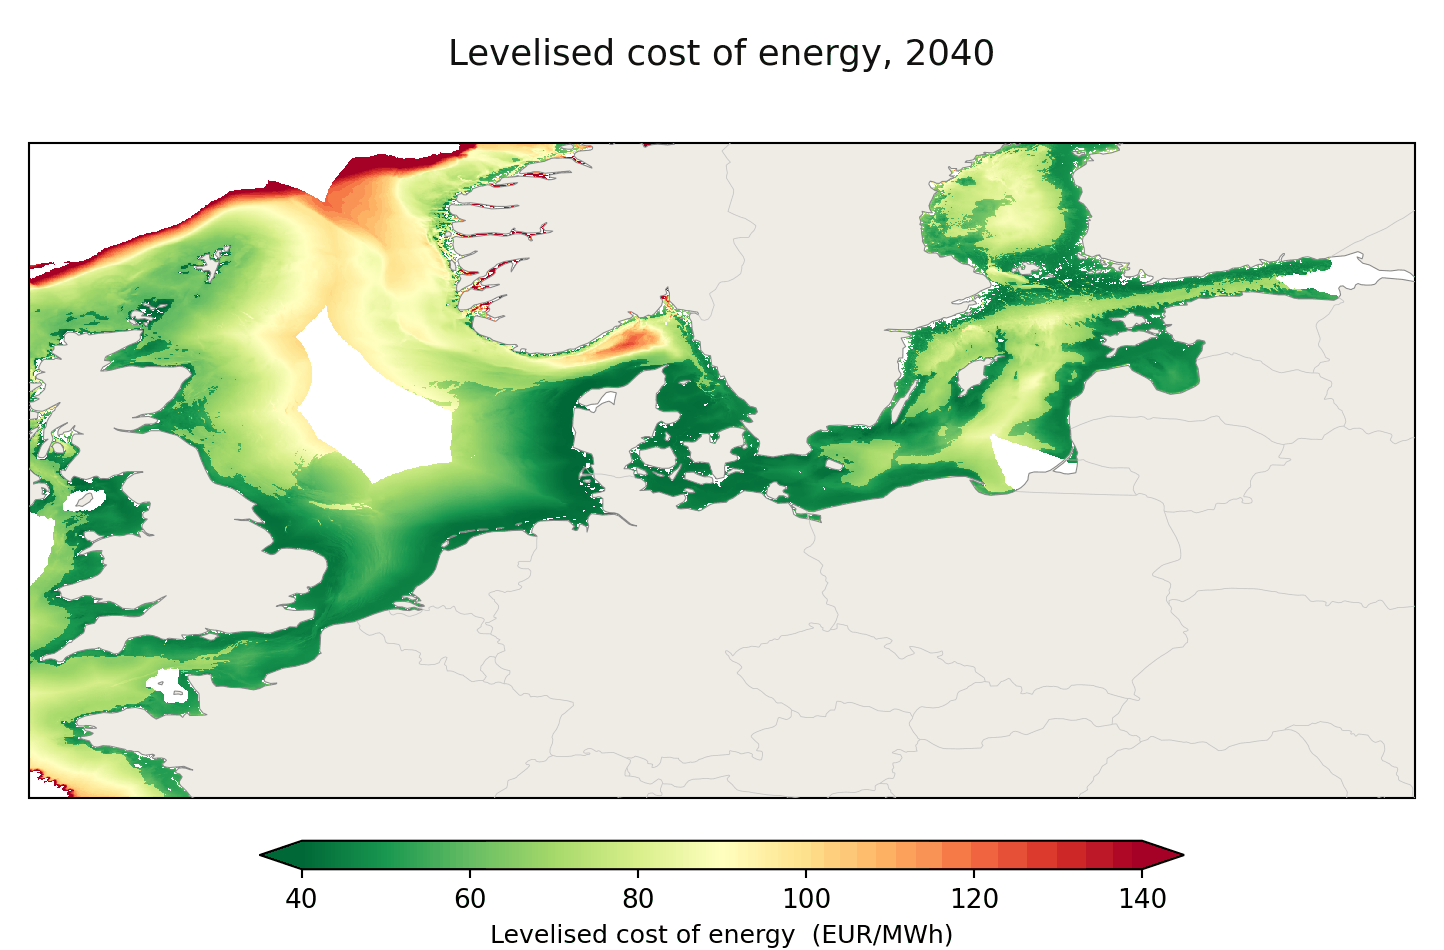
\includegraphics[width=0.72\textwidth]{fig_cost_lcoe_2040}
    \caption{Levelised cost by location, 2040. On cost alone the shelf looks
    steadily more attractive over time, which is precisely the impression the
    value-adjusted maps of Section~F.4 overturn.}
    \label{fig:cost_2040}
\end{figure}

\FloatBarrier
\subsection*{F.4 Value-adjusted cost}

Dividing the cost field by capture value gives the wholesale price a site must
earn to break even (Equation~\ref{eq:vlcoe}). The 2040 map appears in the main
text as Figure~\ref{fig:vlcoe}; the earlier horizons complete the series
and show the direction of travel.

\begin{figure}[!htb]
    \centering
    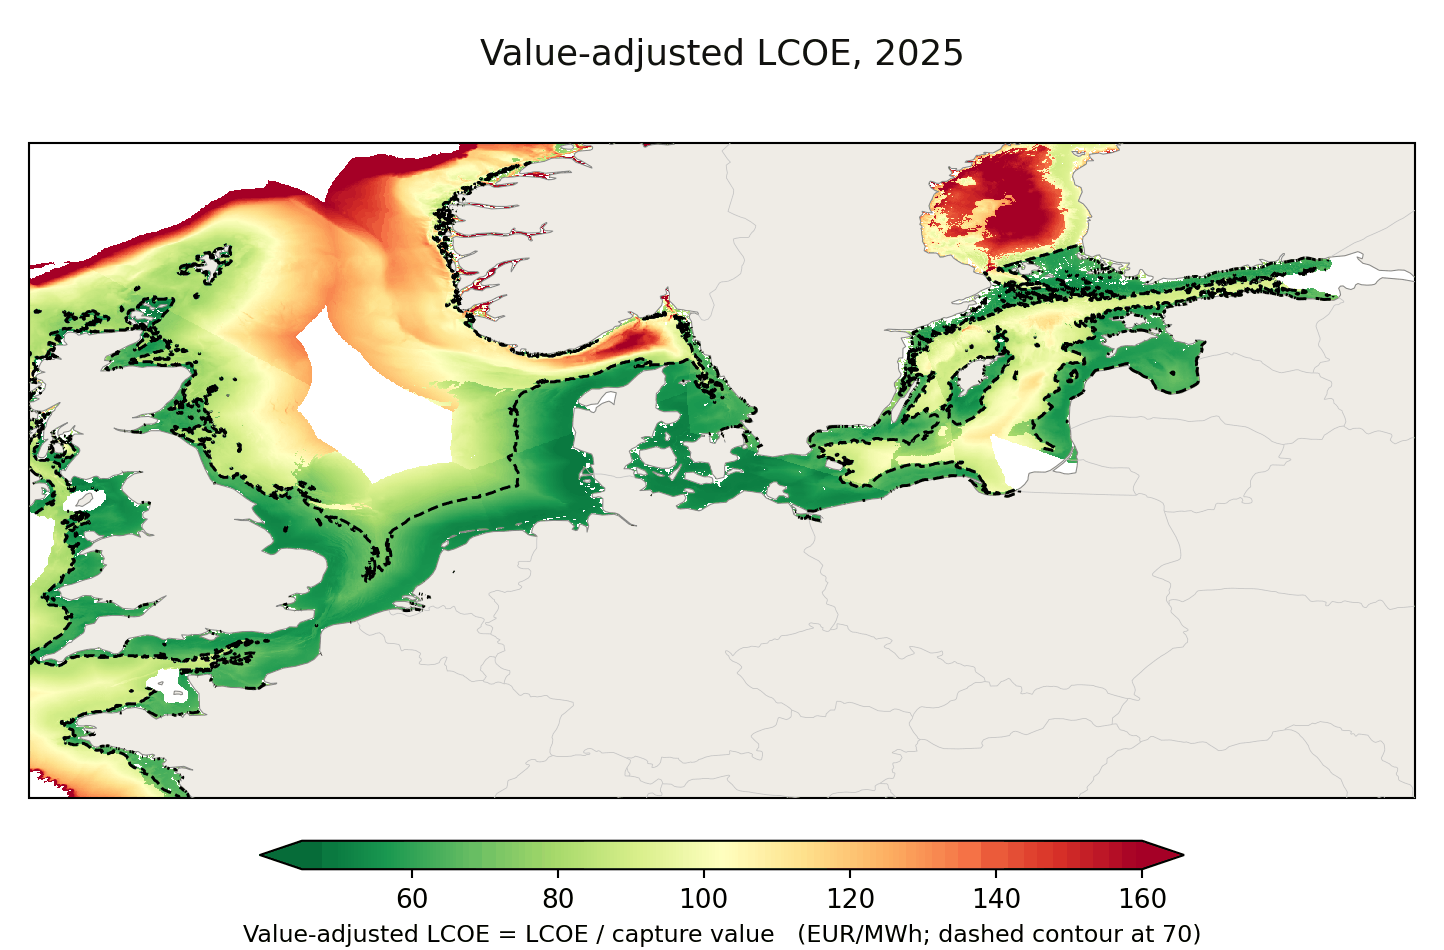
\includegraphics[width=0.72\textwidth]{fig_vlcoe_2025}
    \caption{Value-adjusted cost of energy, 2025. With capture values near 0.9
    across both shelves the field sits close to the raw cost map.}
    \label{fig:vlcoe_2025}
\end{figure}

\begin{figure}[!htb]
    \centering
    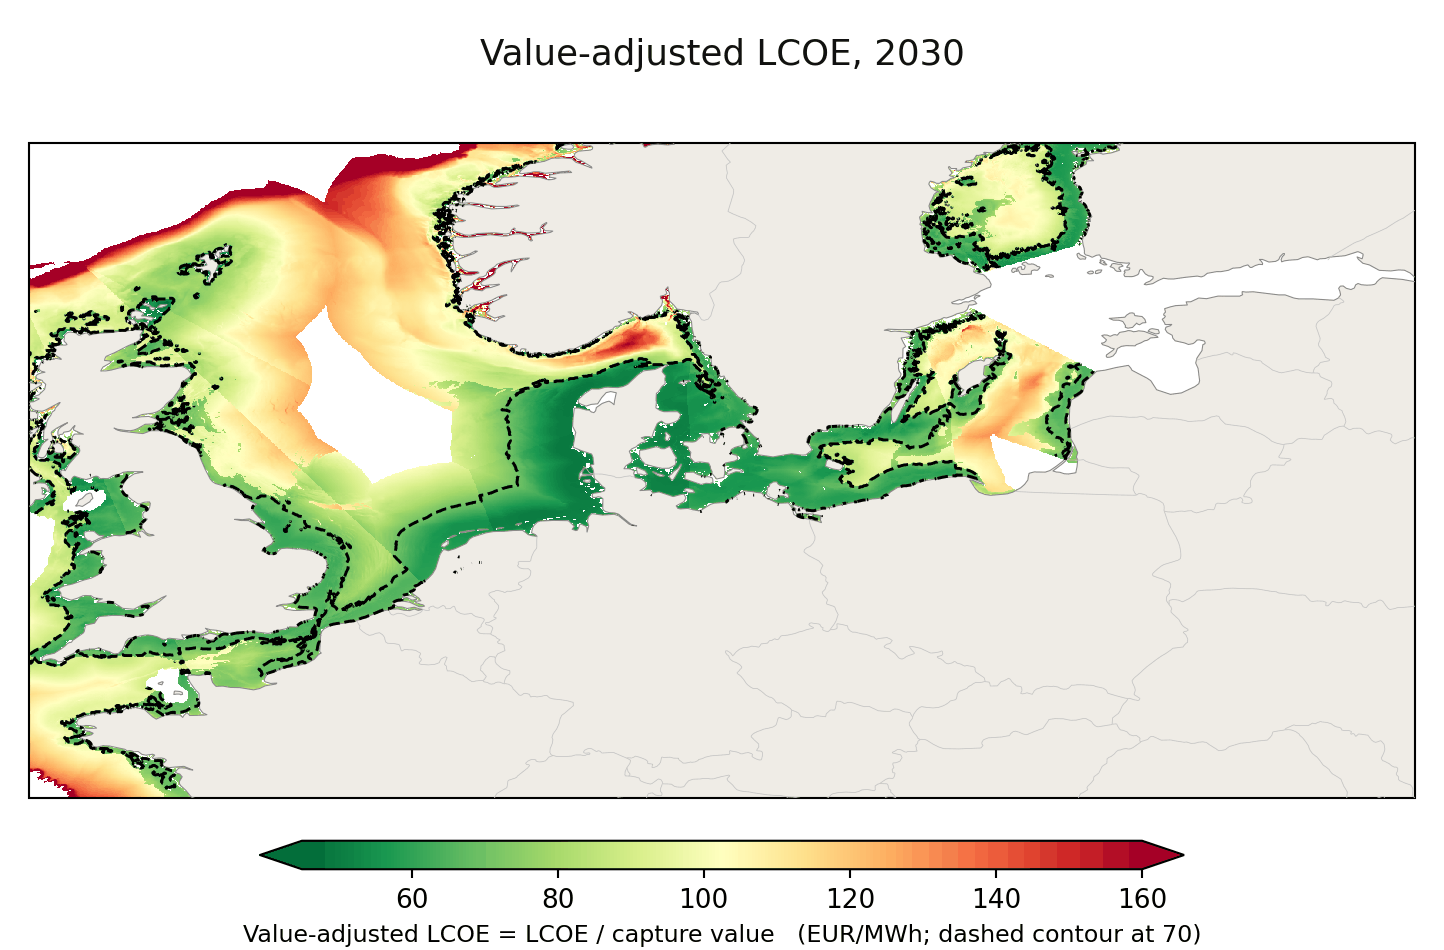
\includegraphics[width=0.72\textwidth]{fig_vlcoe_2030}
    \caption{Value-adjusted cost, 2030. The eastern Baltic begins to separate
    from its cost map as its capture value falls faster than its cost.}
    \label{fig:vlcoe_2030}
\end{figure}

Read against Figures~\ref{fig:cost_2025} to~\ref{fig:cost_2040}, the pair of
series states the thesis result in its most compact form. The cost field
improves monotonically with learning while the value-adjusted field deteriorates,
and the divergence between them is cannibalisation expressed in euros per
megawatt-hour rather than as a ratio.

\FloatBarrier
\subsection*{F.5 Net value}

Net value subtracts annualised cost from revenue and answers whether a site pays
at all, rather than what price it needs. The series opens with the 2040 map
(Figure~\ref{fig:netvalue}), the horizon the body's argument turns on; the
earlier horizons follow.

\begin{figure}[!htb]
    \centering
    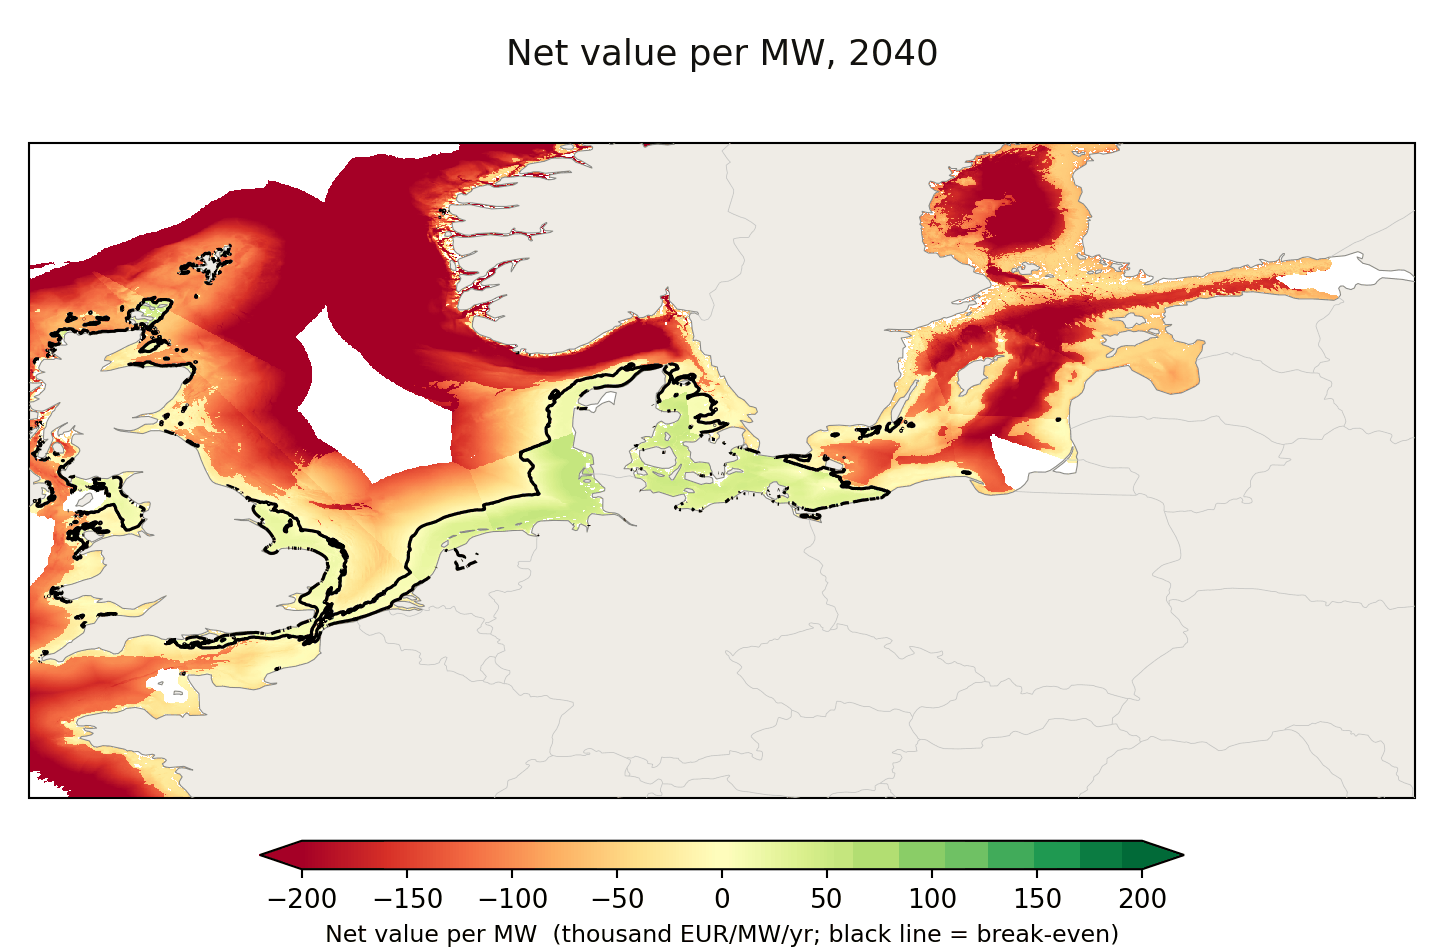
\includegraphics[width=0.6\textwidth]{fig_netvalue_2040}
    \caption{Merchant net value per megawatt in 2040, captured revenue less
    annualised cost. Green is profitable at merchant prices; the profitable shelf
    shrinks from about 48\% of buildable area in 2025 to 12\% by 2040, as value is withdrawn while cost continues to fall.}
    \label{fig:netvalue}
\end{figure}

\begin{figure}[!htb]
    \centering
    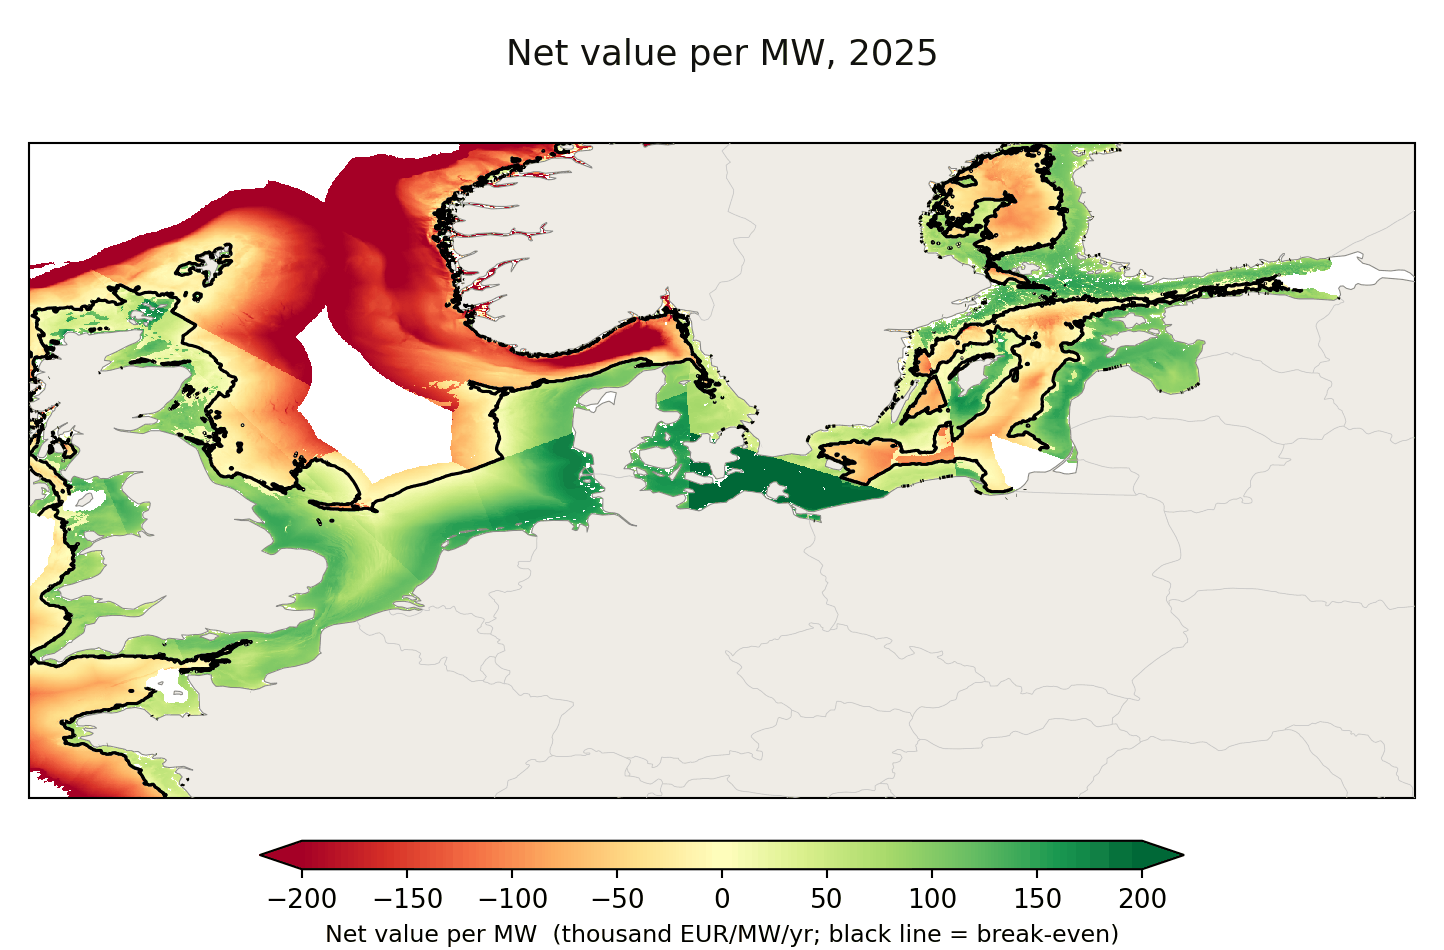
\includegraphics[width=0.72\textwidth]{fig_netvalue_2025}
    \caption{Net value per megawatt, 2025. Roughly half the buildable shelf is
    merchant-profitable at today's capture values and prices.}
    \label{fig:netvalue_2025}
\end{figure}

\begin{figure}[!htb]
    \centering
    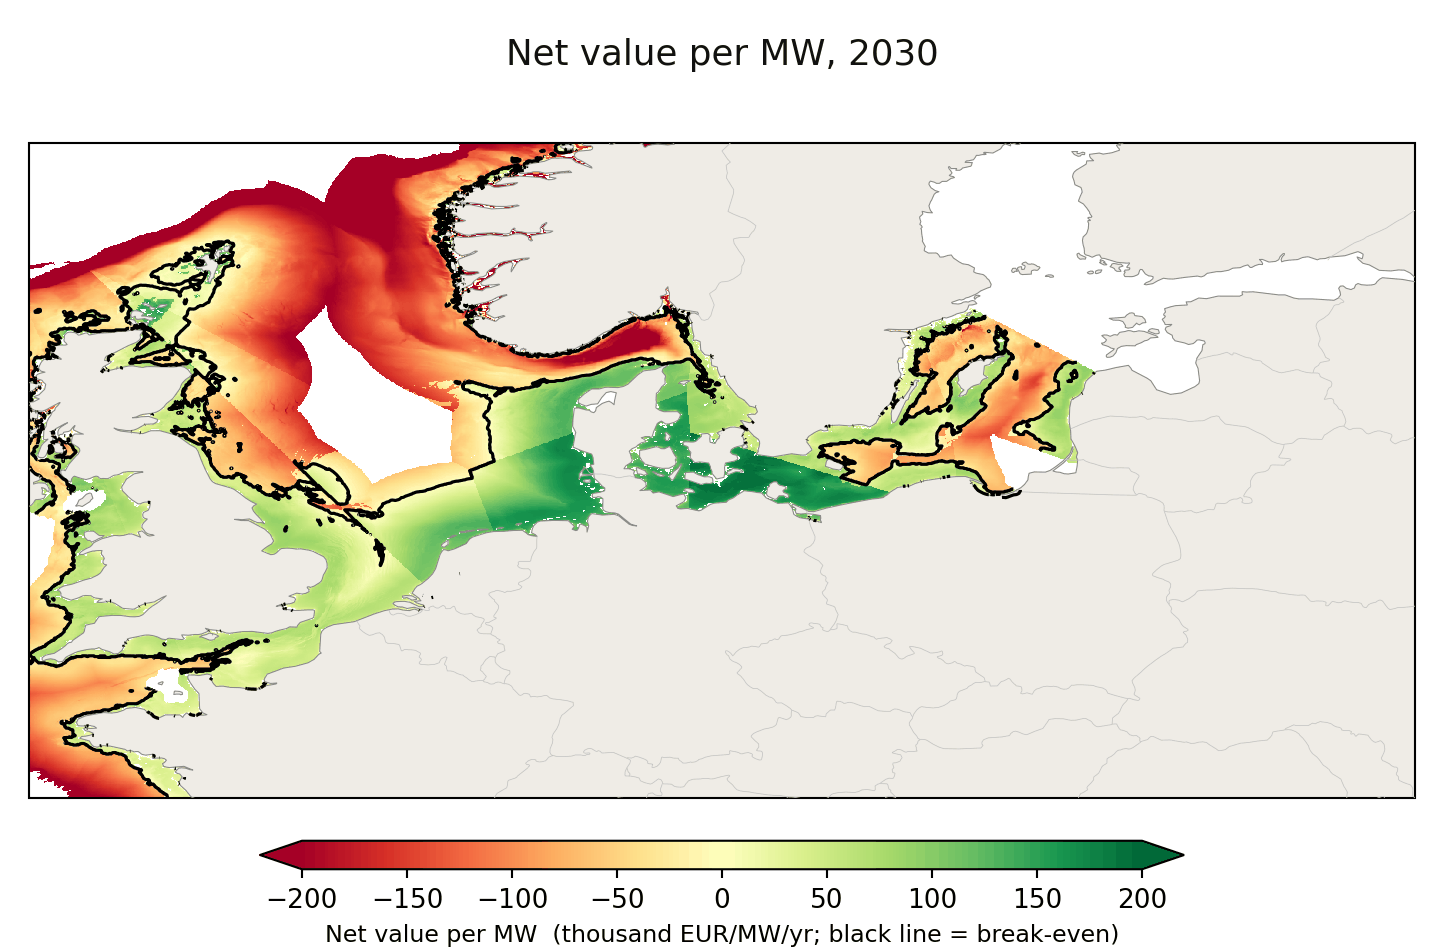
\includegraphics[width=0.72\textwidth]{fig_netvalue_2030}
    \caption{Net value per megawatt, 2030. The profitable area has begun to
    contract toward the shallow, high-resource core.}
    \label{fig:netvalue_2030}
\end{figure}

\FloatBarrier
\subsection*{F.6 Revenue density}

The revenue-density series superimposes the resource field on the per-zone
capture value and price, giving revenue per unit area rather than per megawatt.
It is the most granular of the spatial products, built on the roughly 2~km Global
Wind Atlas field.

\begin{figure}[!htb]
    \centering
    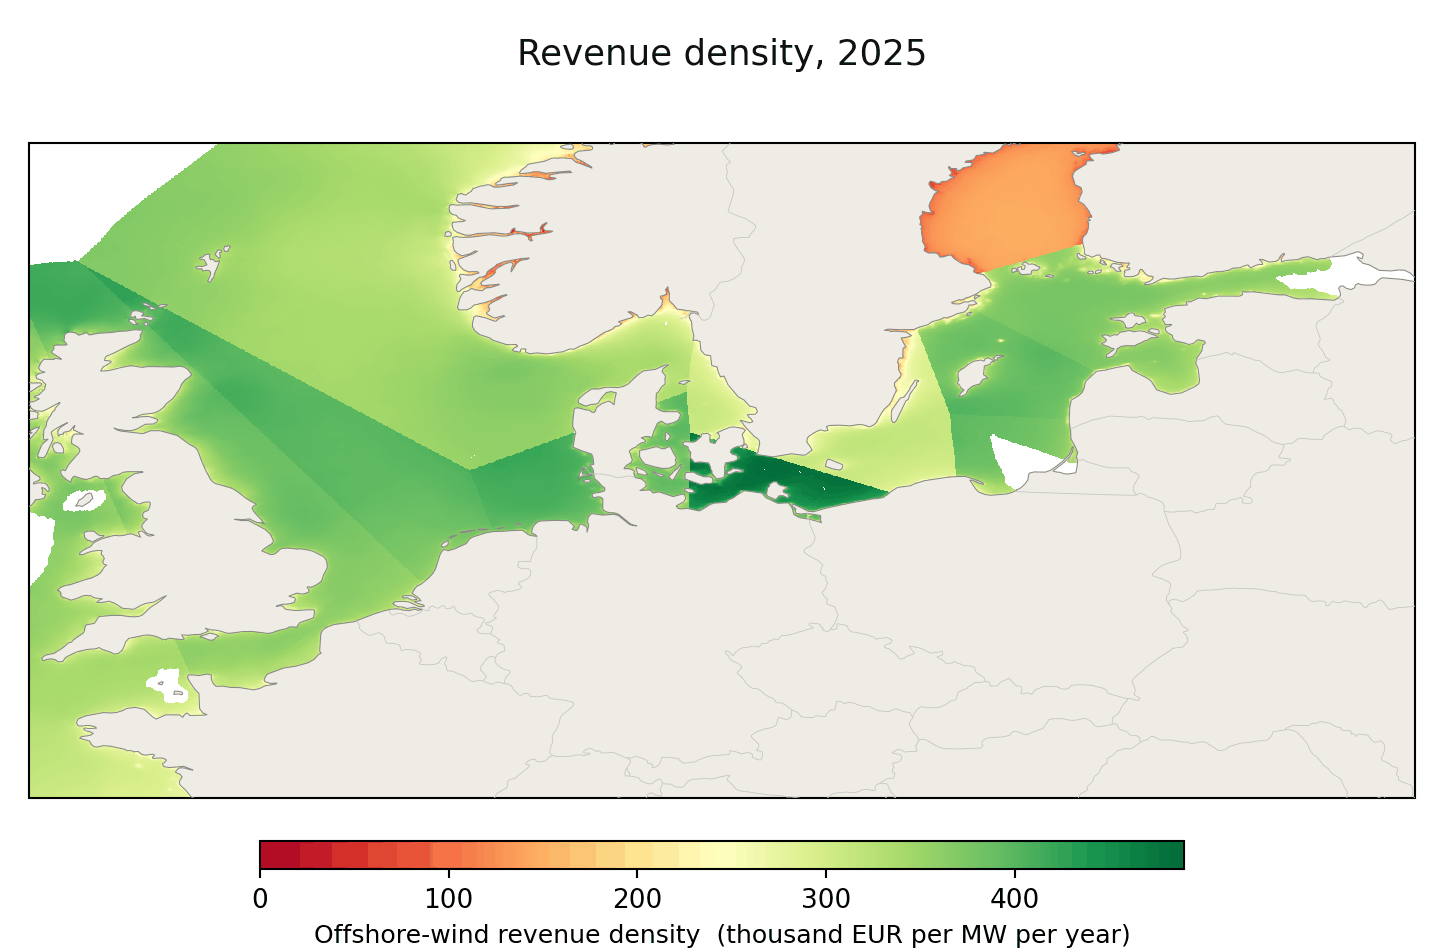
\includegraphics[width=0.72\textwidth]{fig_revenue_density_hires_2025}
    \caption{Revenue density across both shelves, 2025.}
    \label{fig:revdens_2025}
\end{figure}

\begin{figure}[!htb]
    \centering
    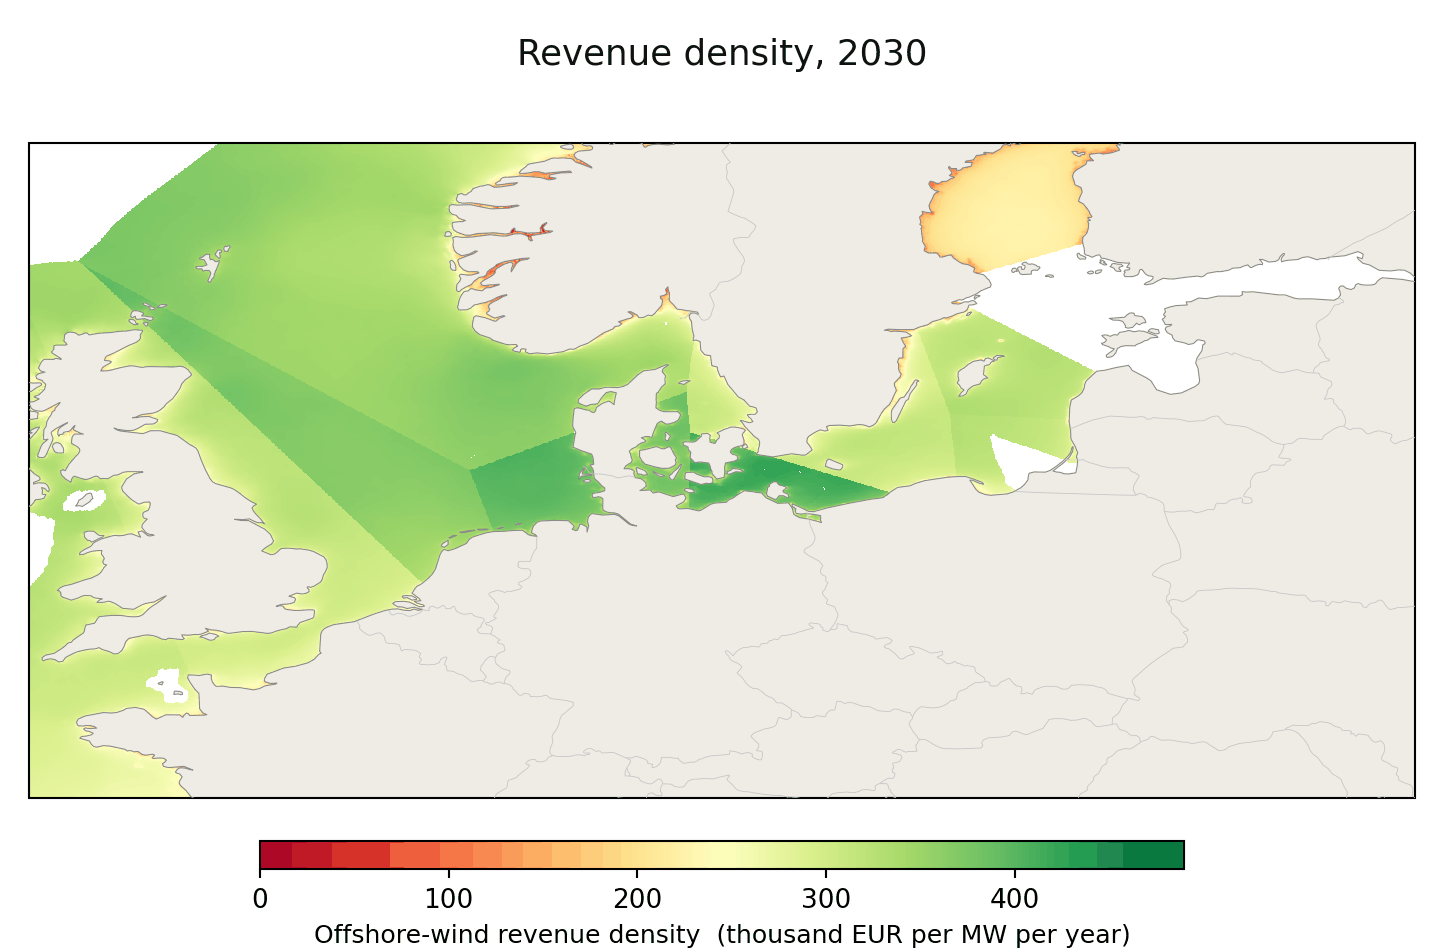
\includegraphics[width=0.72\textwidth]{fig_revenue_density_hires_2030}
    \caption{Revenue density, 2030.}
    \label{fig:revdens_2030}
\end{figure}

\begin{figure}[!htb]
    \centering
    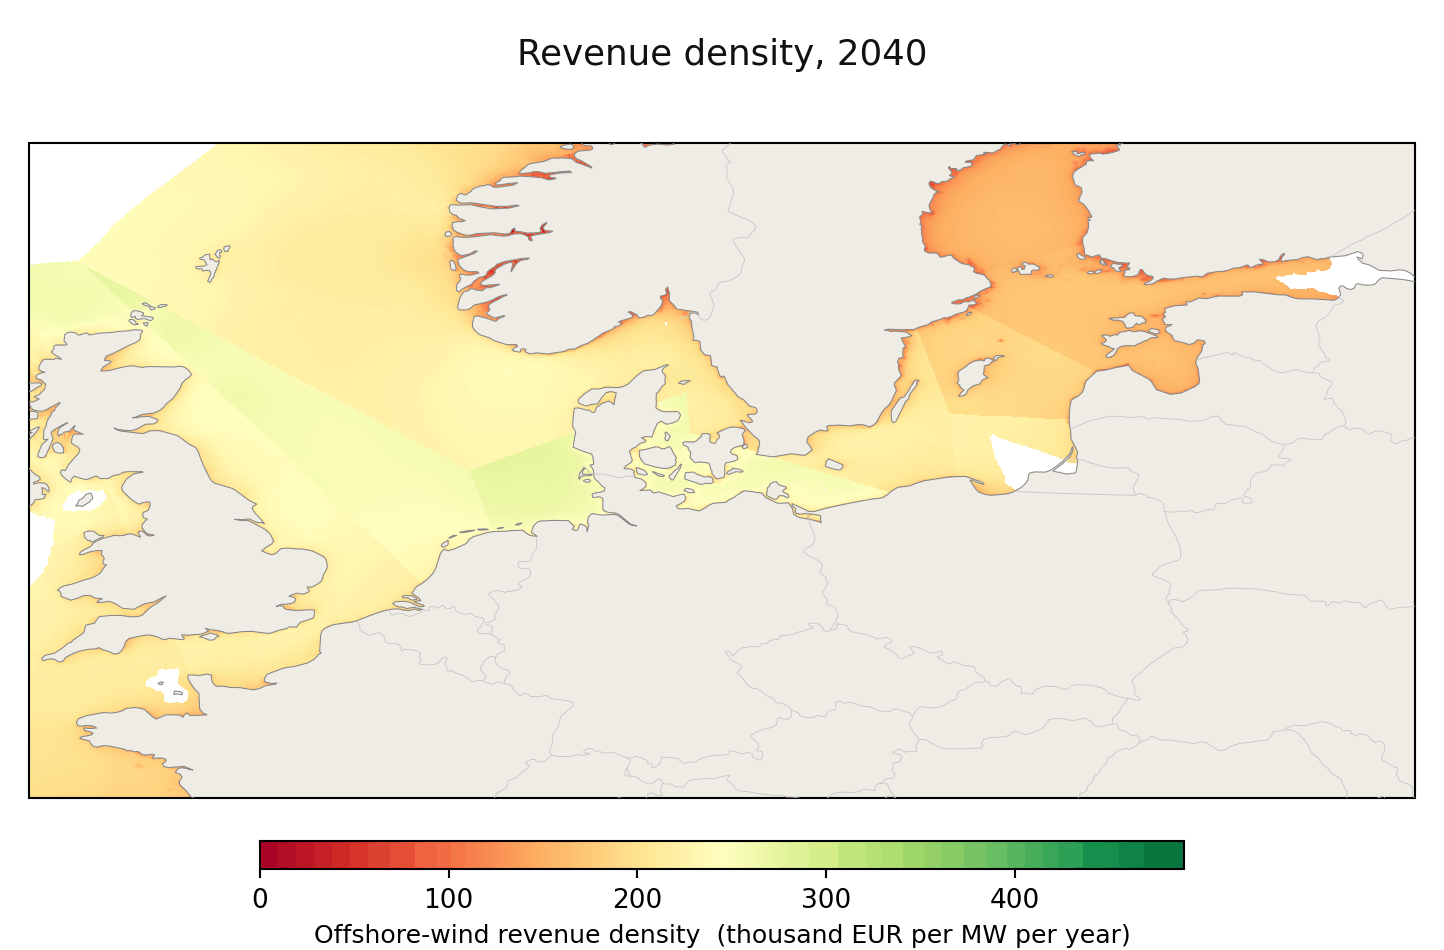
\includegraphics[width=0.72\textwidth]{fig_revenue_density_hires_2040}
    \caption{Revenue density, 2040. The contraction toward the German Bight and
    the shallow western Baltic is the same pattern the site ranking of
    Section~\ref{sec:site_ranking} produces numerically.}
    \label{fig:revdens_2040}
\end{figure}

\FloatBarrier
\subsection*{F.7 Candidate areas on the value grid}

\begin{figure}[!htb]
    \centering
    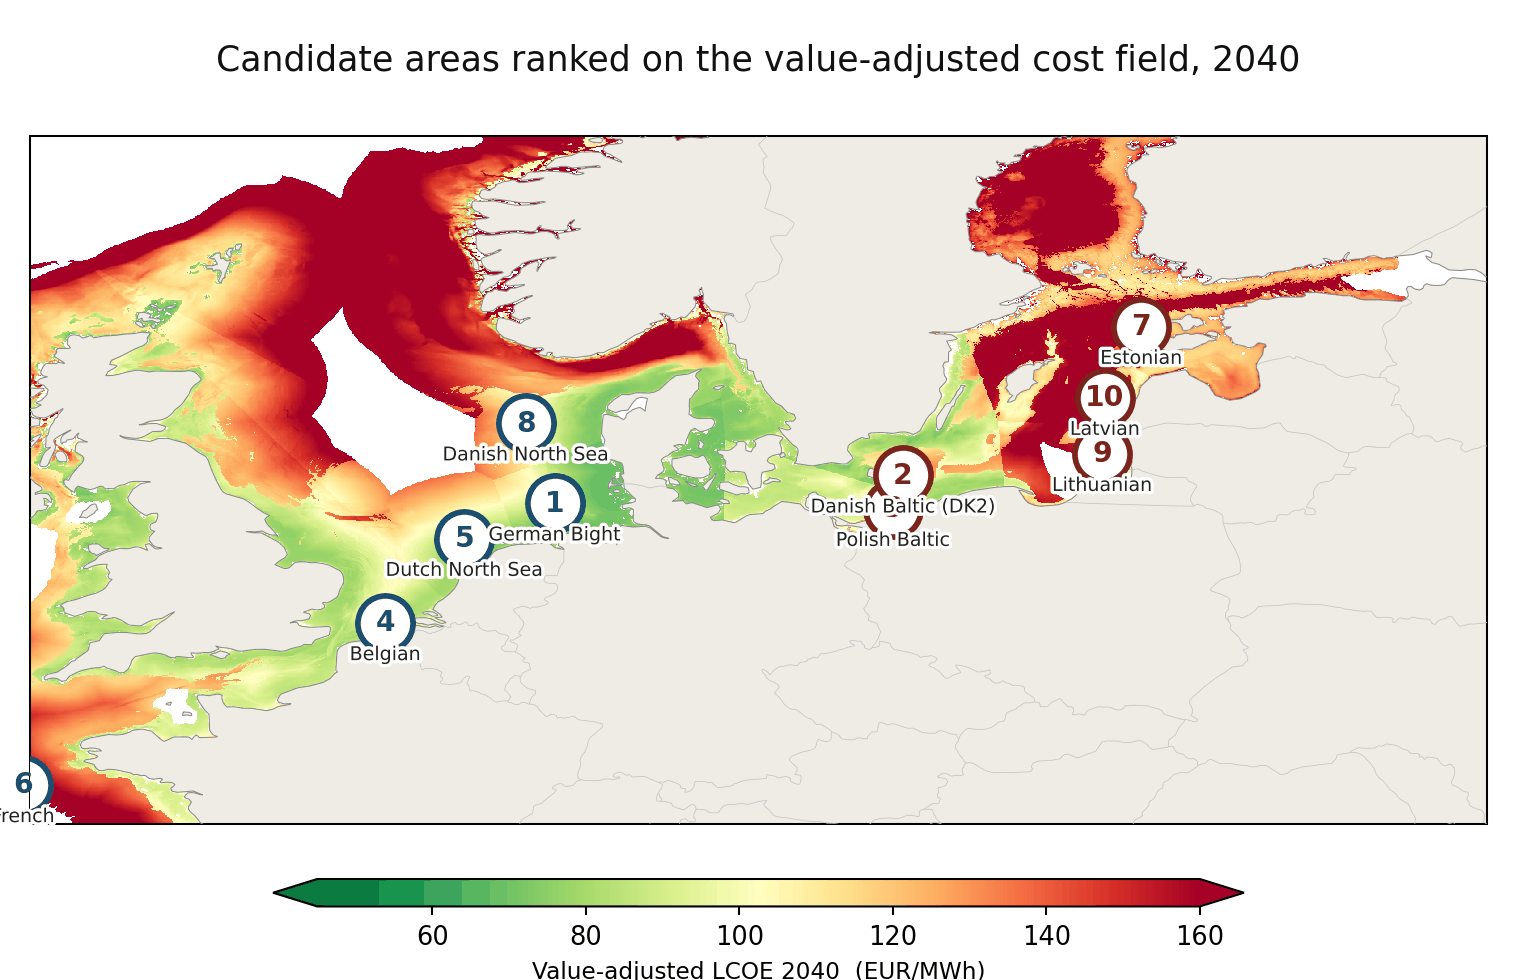
\includegraphics[width=0.86\textwidth]{fig_site_ranking_map}
    \caption{The ten candidate development areas positioned on the 2040
    value-adjusted field, which is the spatial backing for the ranking reported
    in Section~\ref{sec:site_ranking}. Circled numbers give the value-adjusted
    rank, 1 the best; blue marks North Sea areas, red Baltic. The areas that
    fall in the ranking are visibly those sitting in the reddest water.}
    \label{fig:site_ranking_map}
\end{figure}

% ============================================================================
\FloatBarrier
\section{Supplementary Figures}\label{app:supplementary}
% ============================================================================

This appendix holds diagnostics and intermediate results referenced in passing by
the main text, grouped by the chapter they support.

\FloatBarrier
\subsection*{G.1 Model resolution}



\begin{figure}[!htb]
    \centering
    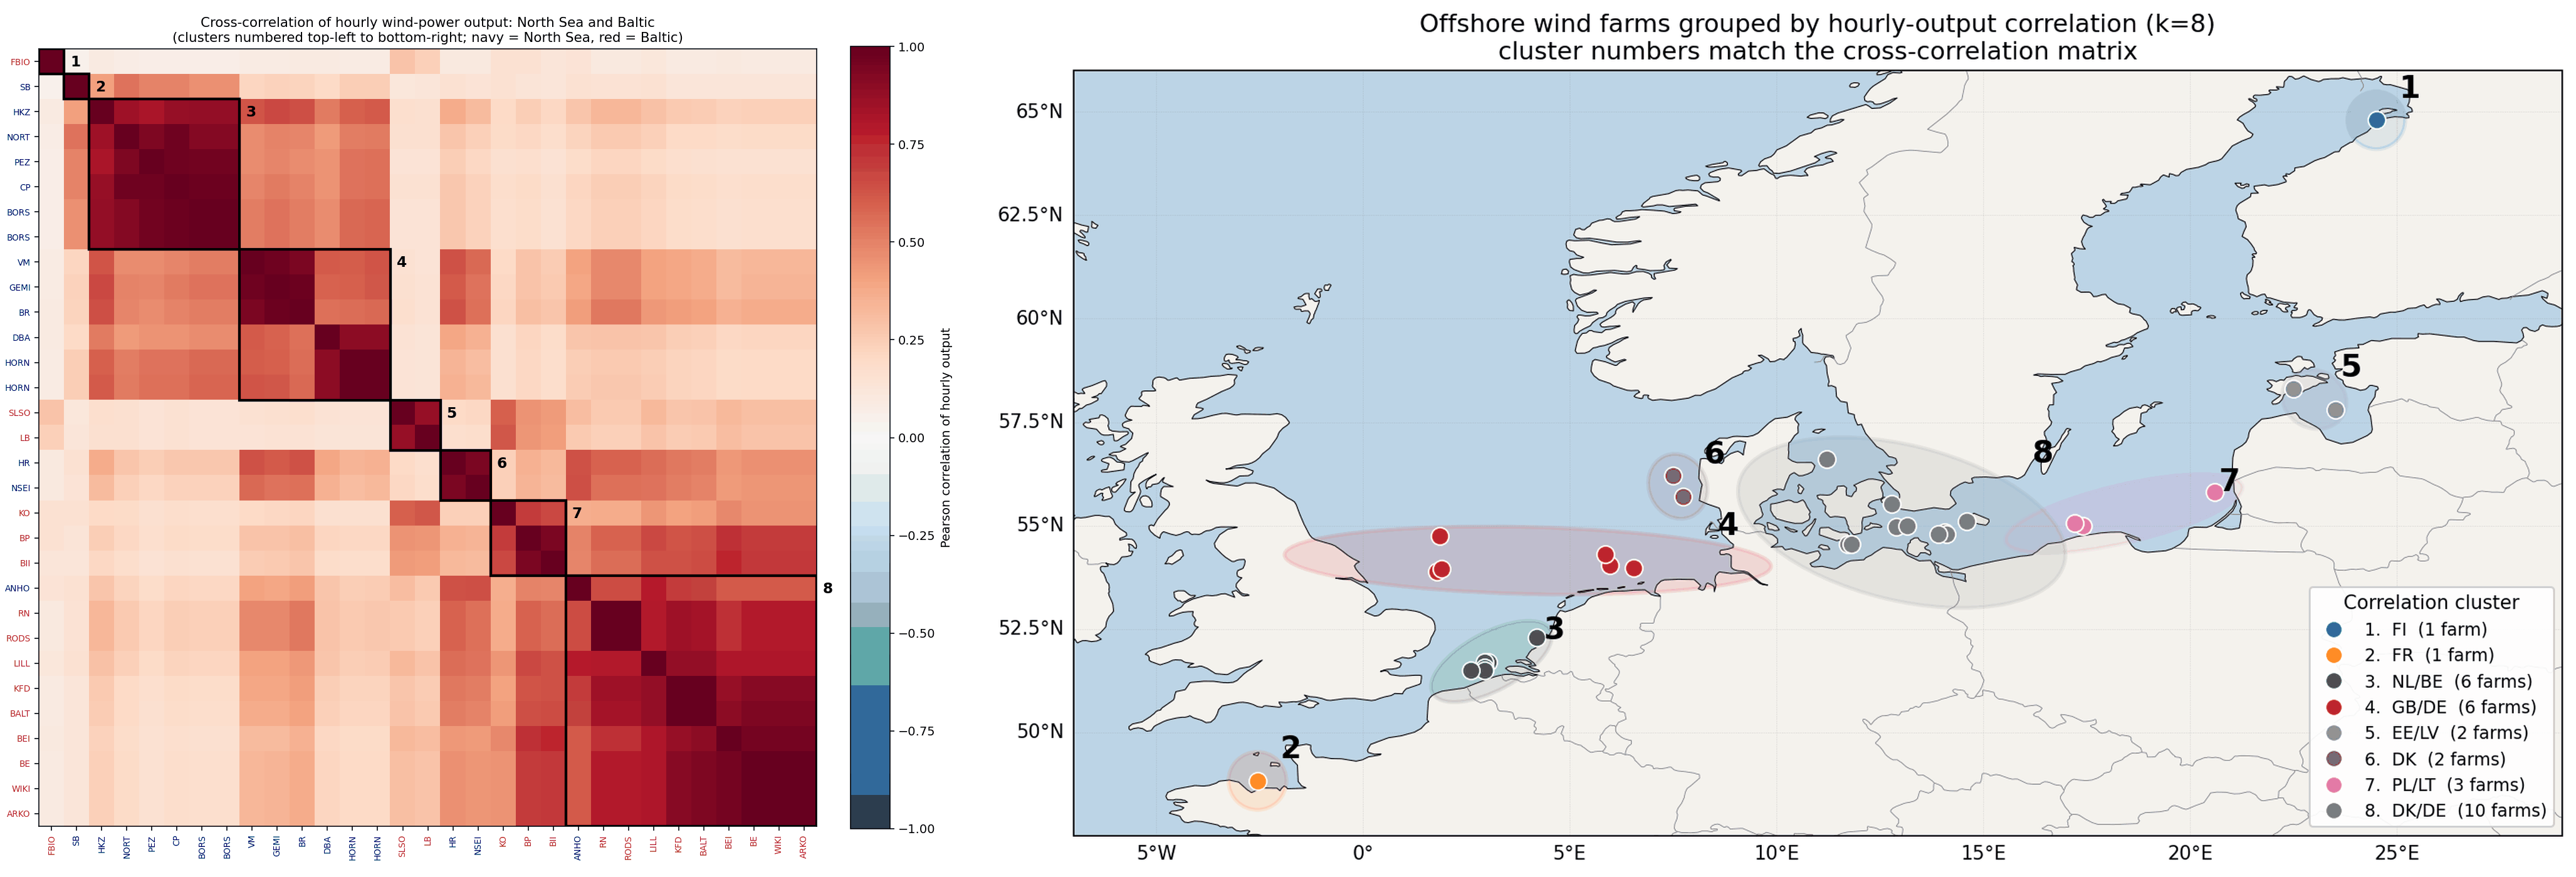
\includegraphics[width=0.80\textwidth]{fig_clusters_matrix_map}
    \caption{The 30-node clustering of the study region, showing which physical
    buses are aggregated into each model node. Copper-plating within a node is
    the limitation this resolution imposes, and the reason small well-connected
    zones carry the largest system-model bias.}
    \label{fig:clusters_map}
\end{figure}

\FloatBarrier
\subsection*{G.2 Measured capture value}

\begin{figure}[!htb]
    \centering
    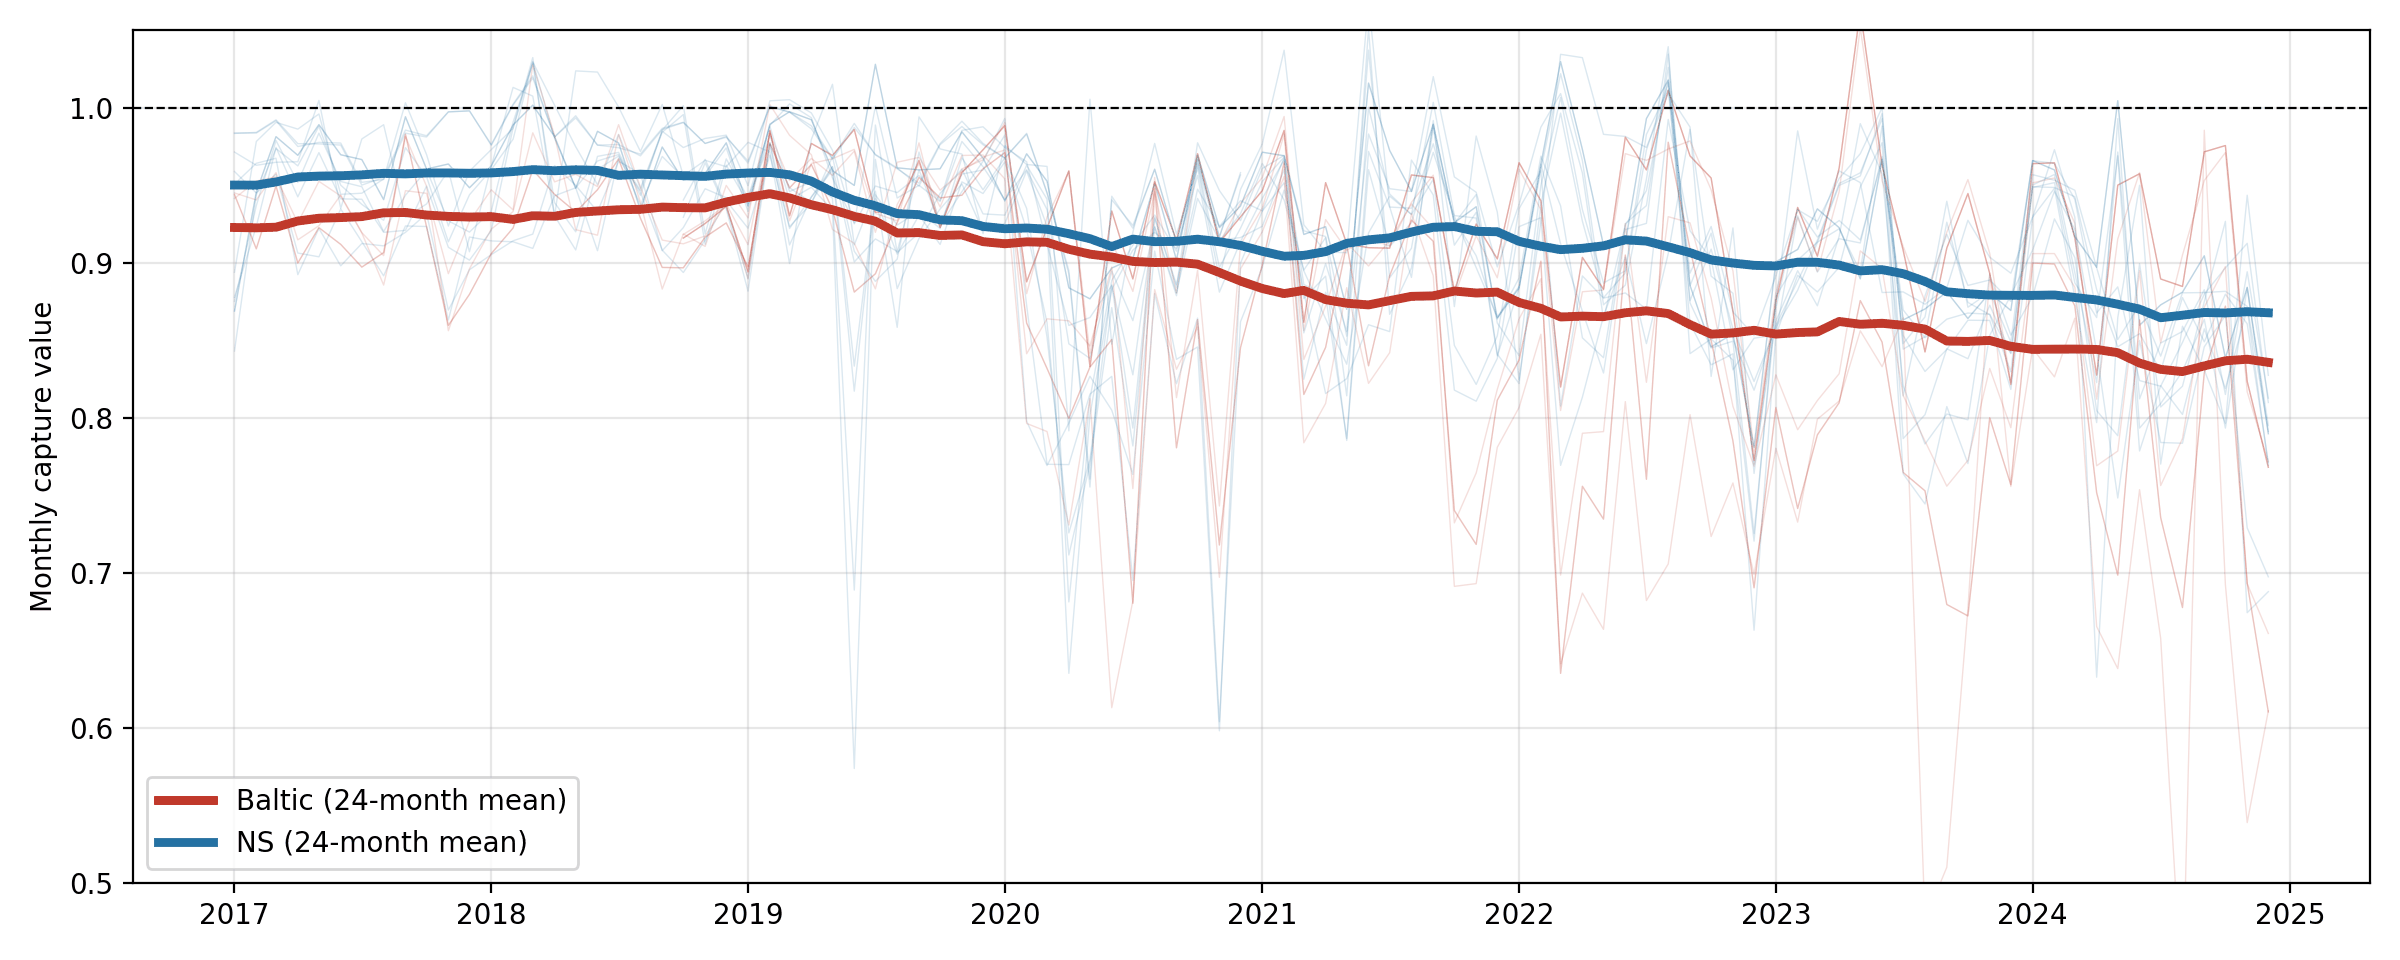
\includegraphics[width=0.88\textwidth]{fig_B_cv_history_basins}
    \caption{Eight years of measured capture value by basin, the full history
    behind the summary in Section~\ref{sec:eight_years}.}
    \label{fig:cv_history}
\end{figure}


\begin{figure}[!htb]
    \centering
    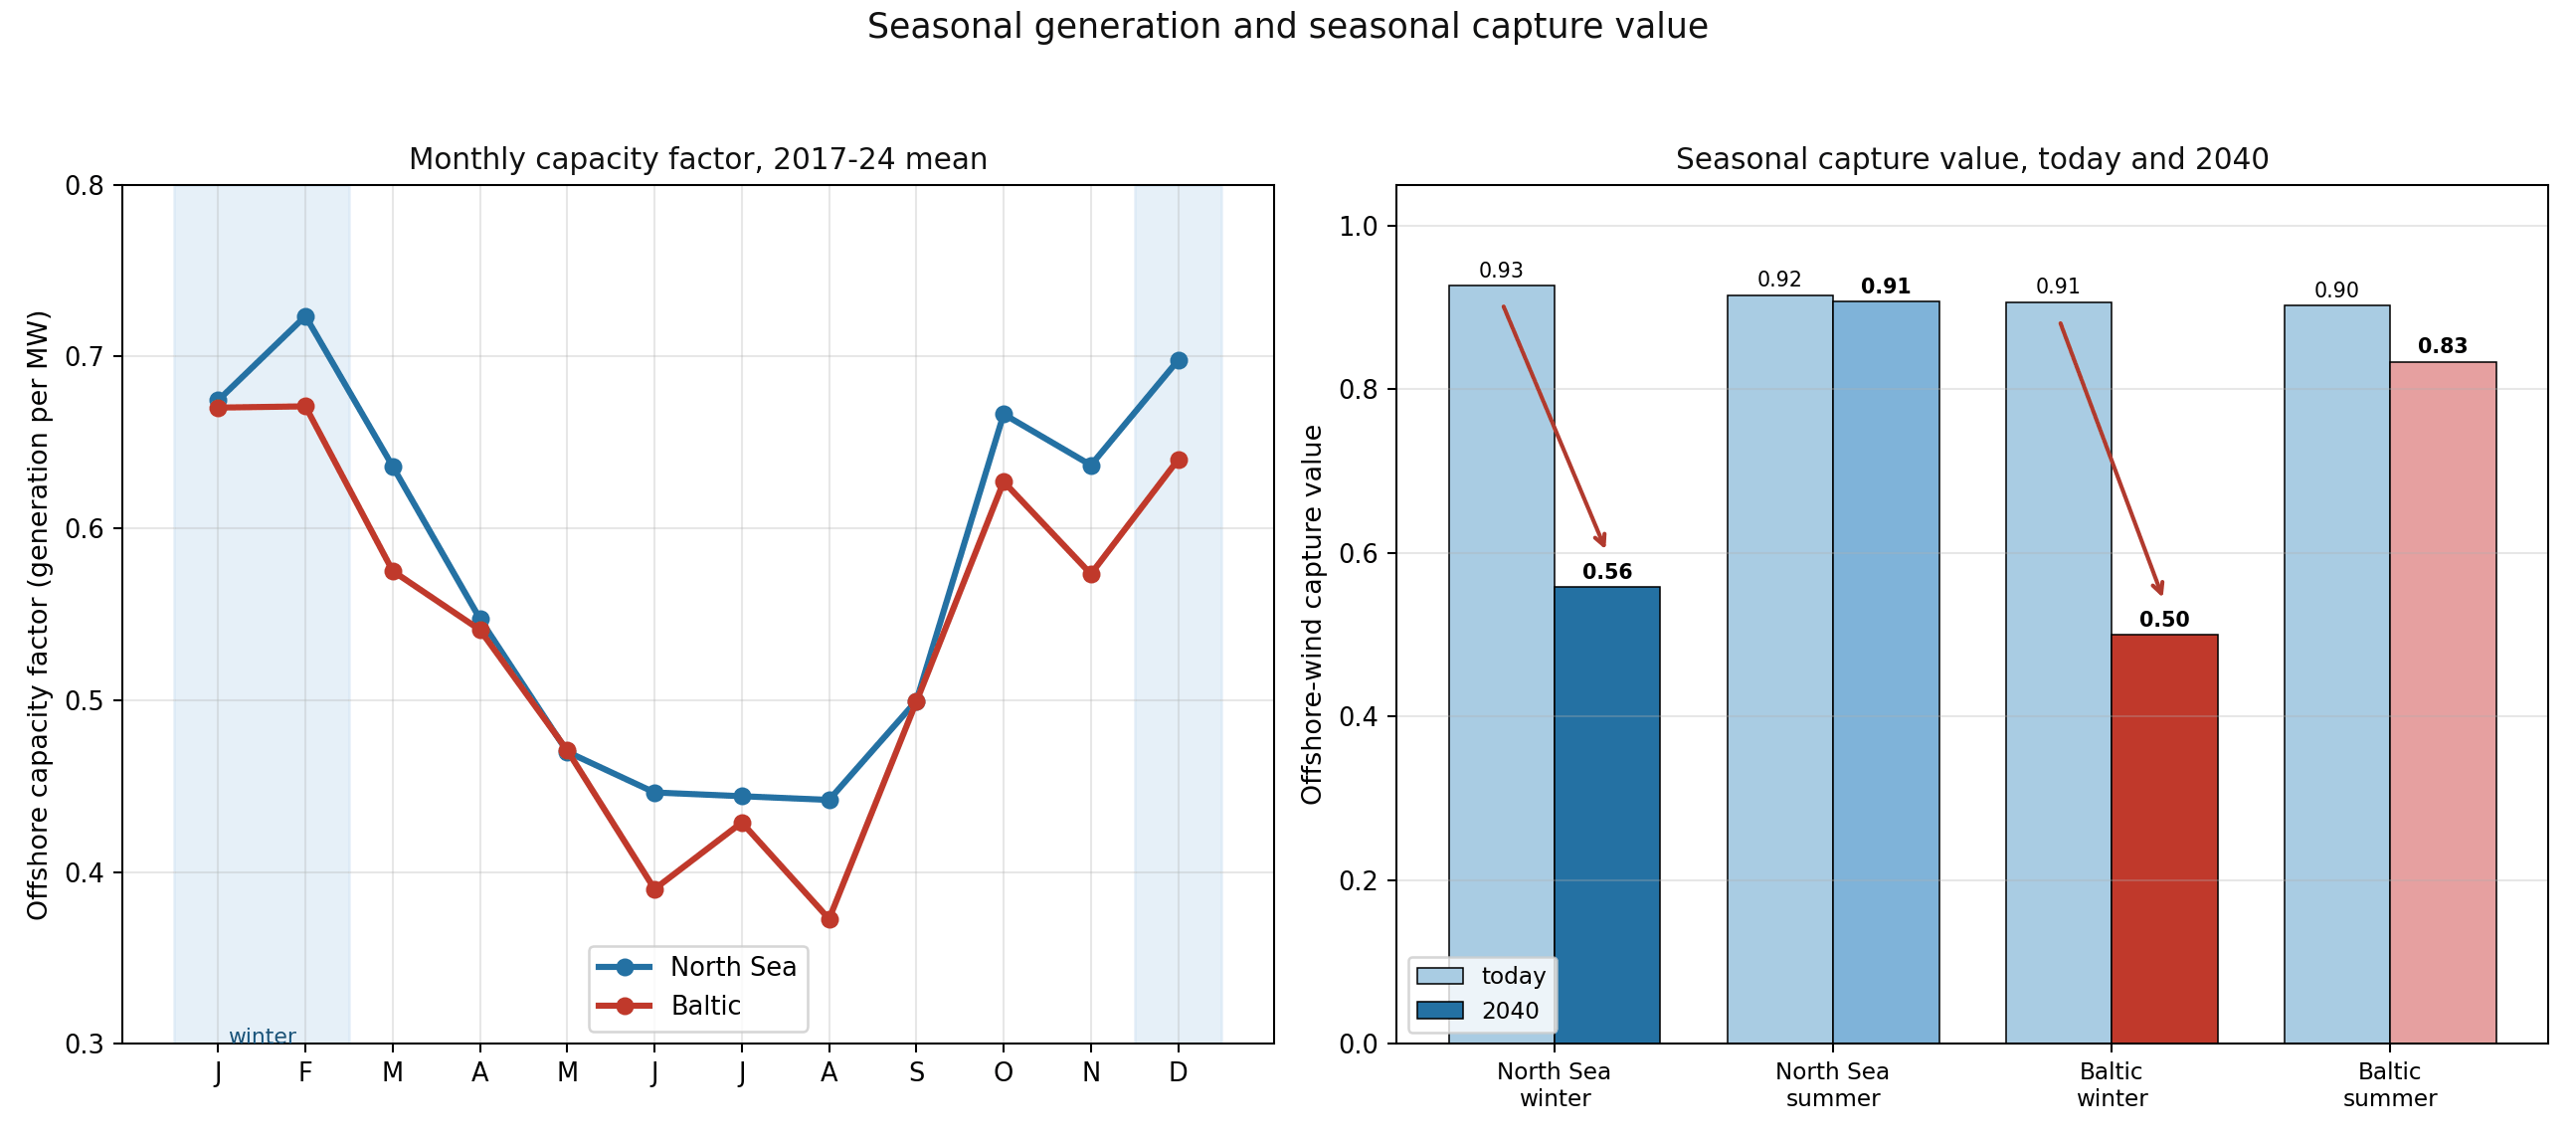
\includegraphics[width=0.88\textwidth]{fig_seasonal_generation}
    \caption{The seasonal generation profile and its interaction with capture
    value: output peaks in winter, which is also when the basins synchronise, so
    the largest volumes are sold into the most depressed hours.}
    \label{fig:seasonal_generation}
\end{figure}


\begin{figure}[!htb]
    \centering
    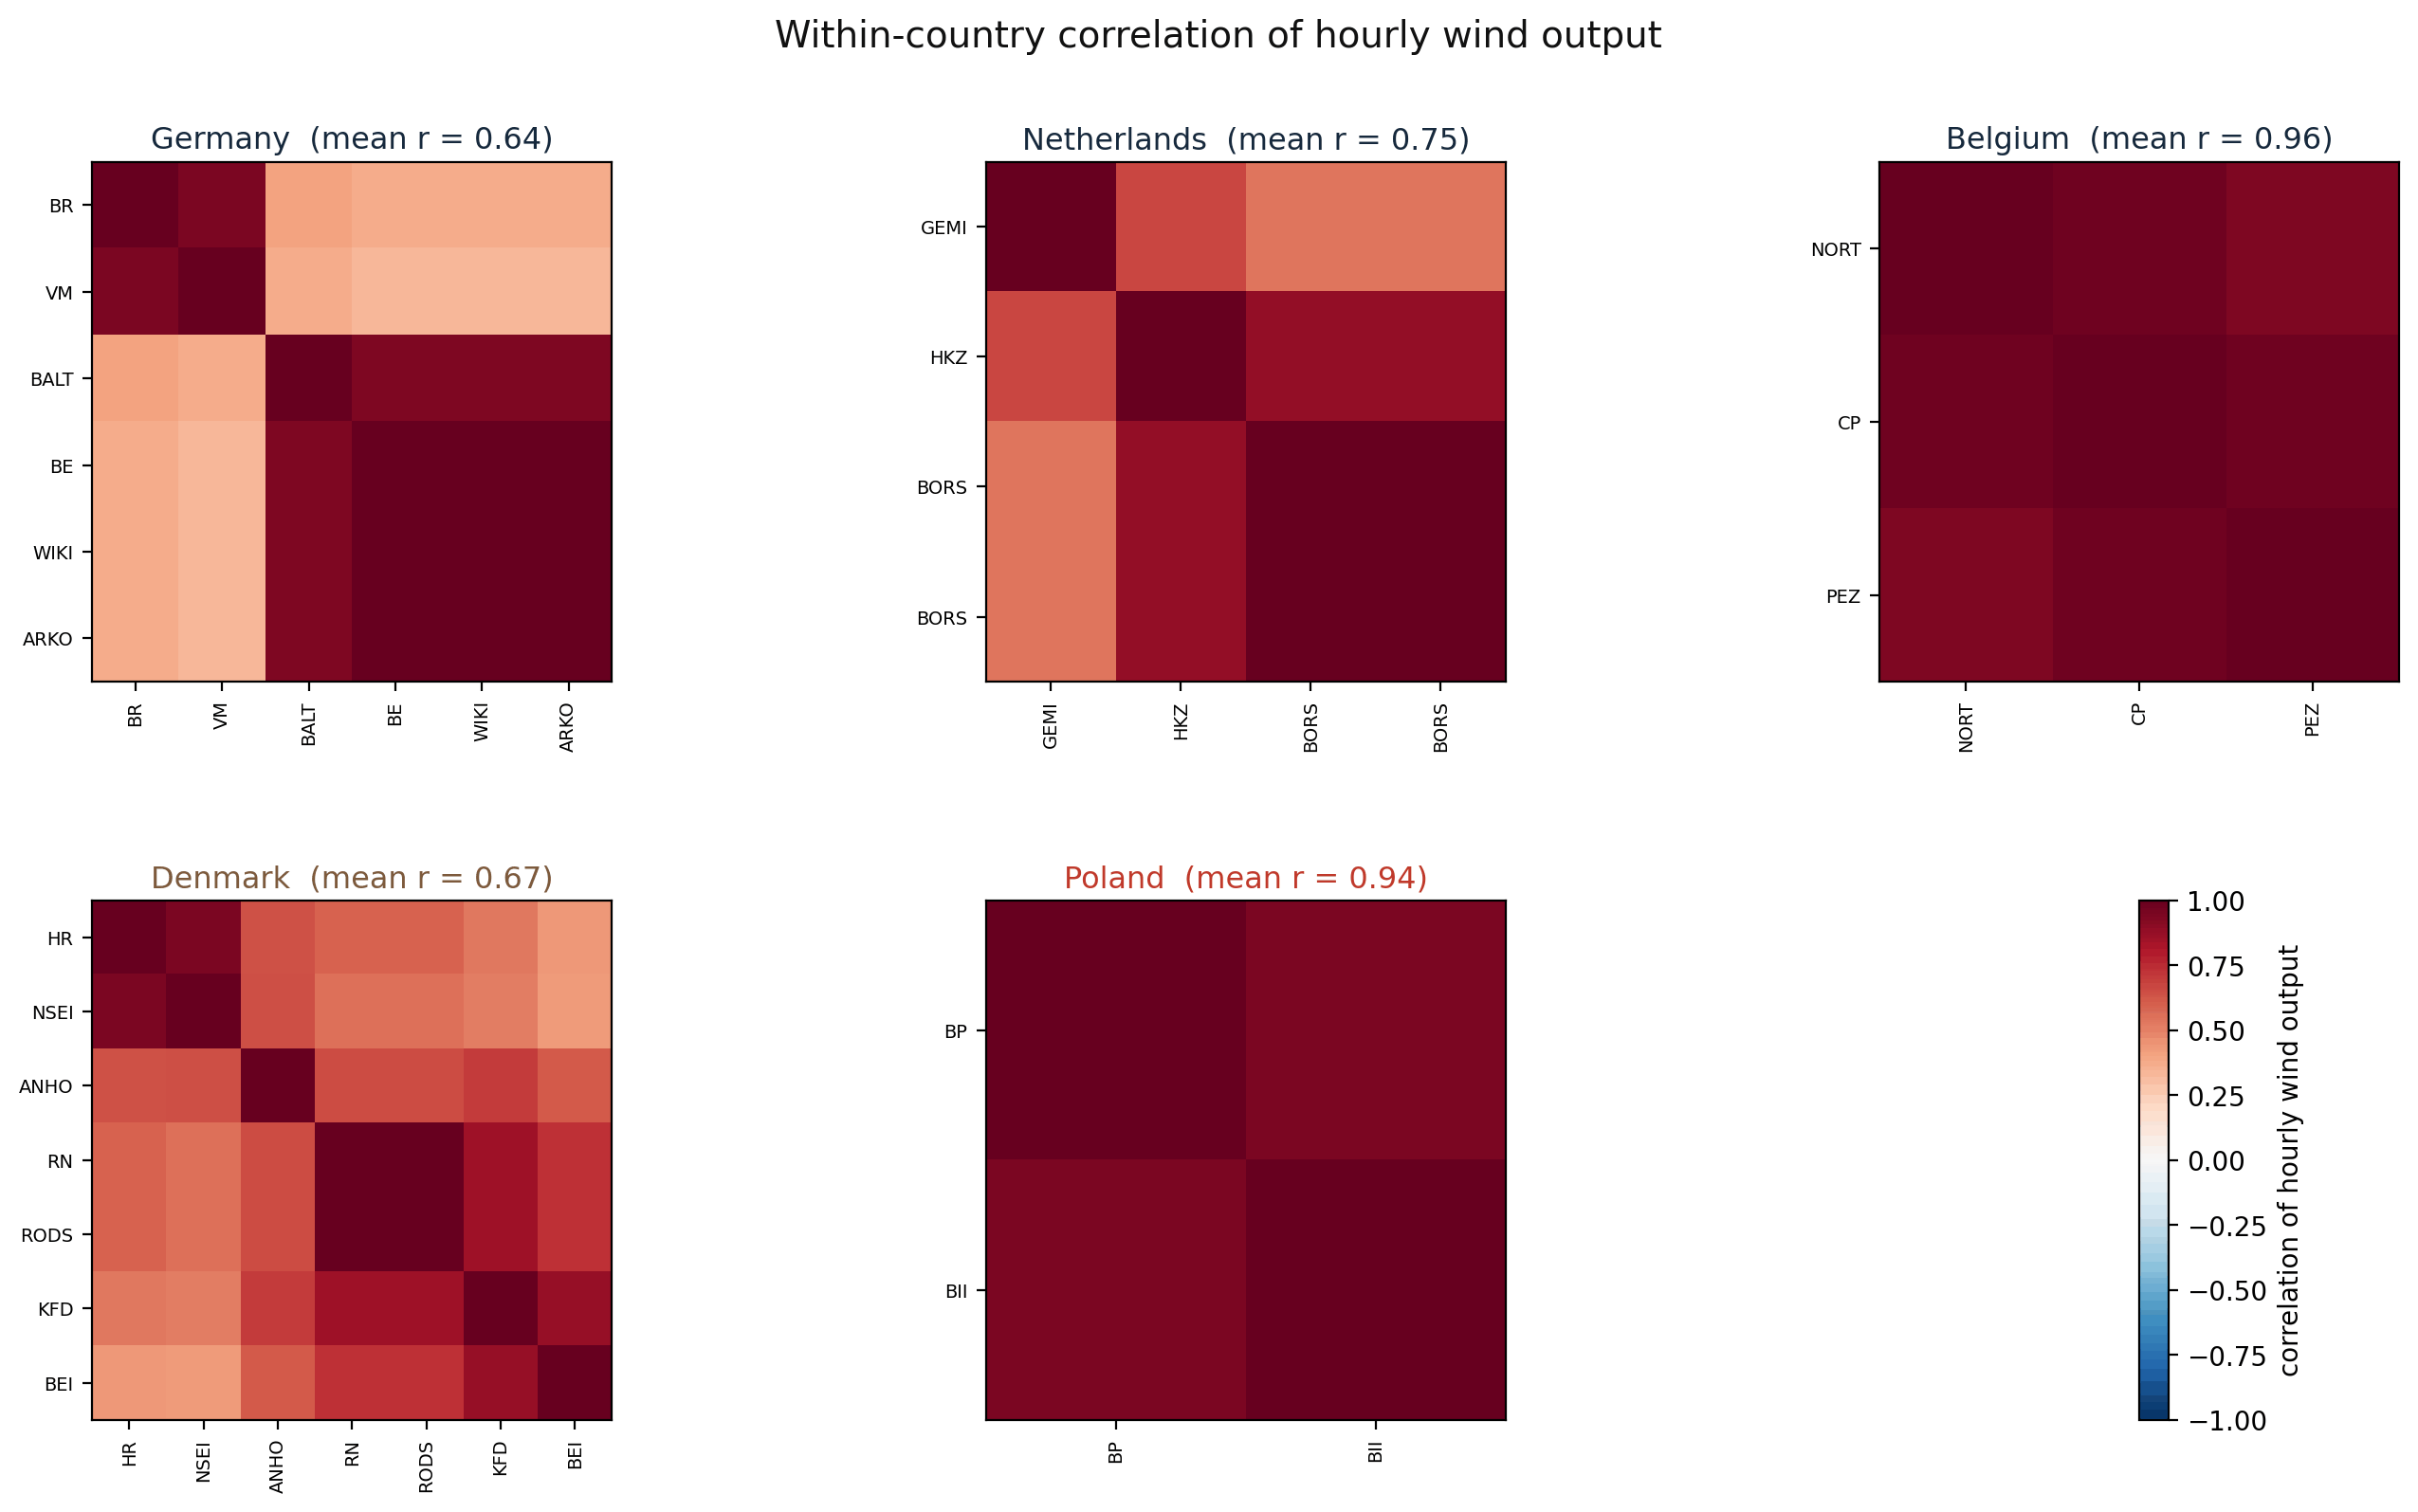
\includegraphics[width=0.88\textwidth]{fig_country_correlation}
    \caption{Within-country wind synchronicity matrices, the granular analogue
    of the basin correlation figure. Compact fleets blow nearly as one (Belgium
    0.96, Poland 0.94); spread fleets do not (Germany 0.64, Denmark 0.67).
    Germany splits into two blocks, its North Sea and Baltic farms, so the basin boundary dominates the national one.}
    \label{fig:country_correlation}
\end{figure}

\FloatBarrier
\subsection*{G.3 Within-Baltic convergence}



\begin{figure}[!htb]
    \centering
    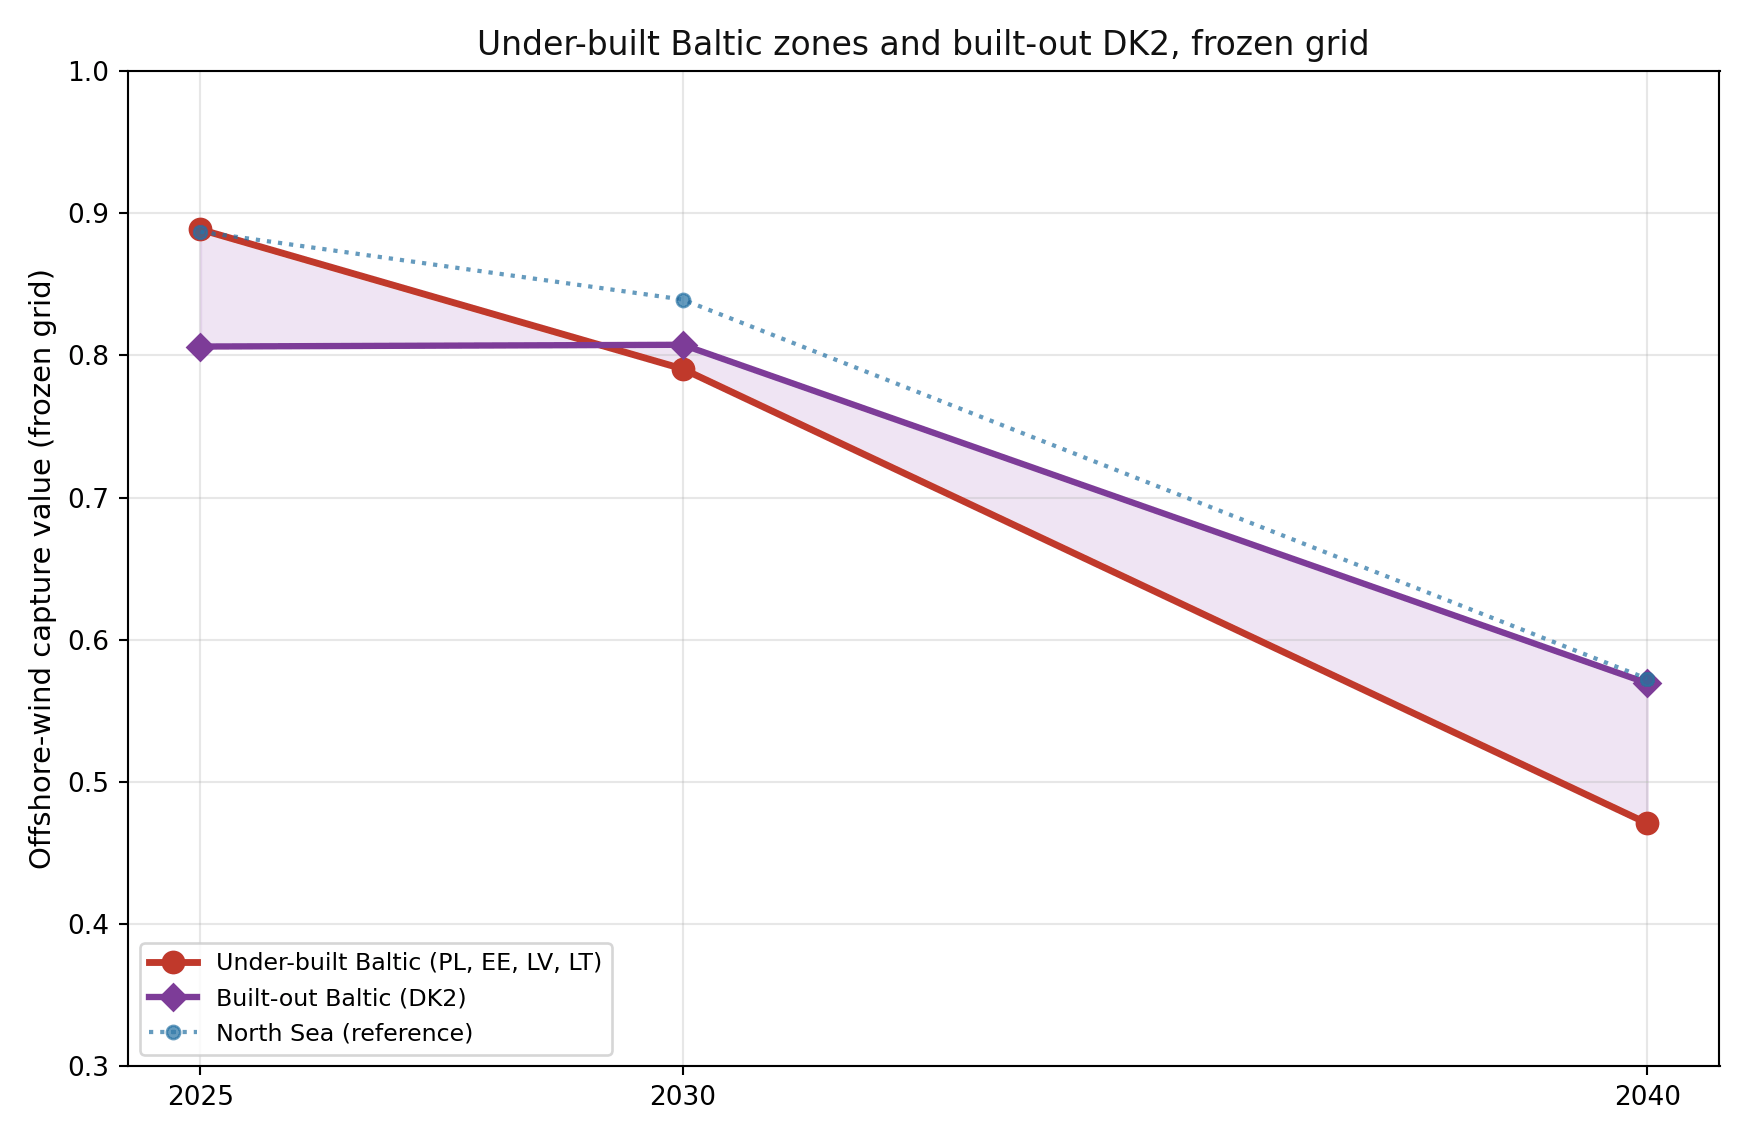
\includegraphics[width=0.88\textwidth]{fig_baltic_convergence}
    \caption{Convergence of the under-built Baltic zones onto the values already
    reached by the built-out DK2 and SE4, the space-for-time argument shown
    directly.}
    \label{fig:baltic_convergence}
\end{figure}




\FloatBarrier
\subsection*{G.4 Model diagnostics}



\begin{figure}[!htb]
    \centering
    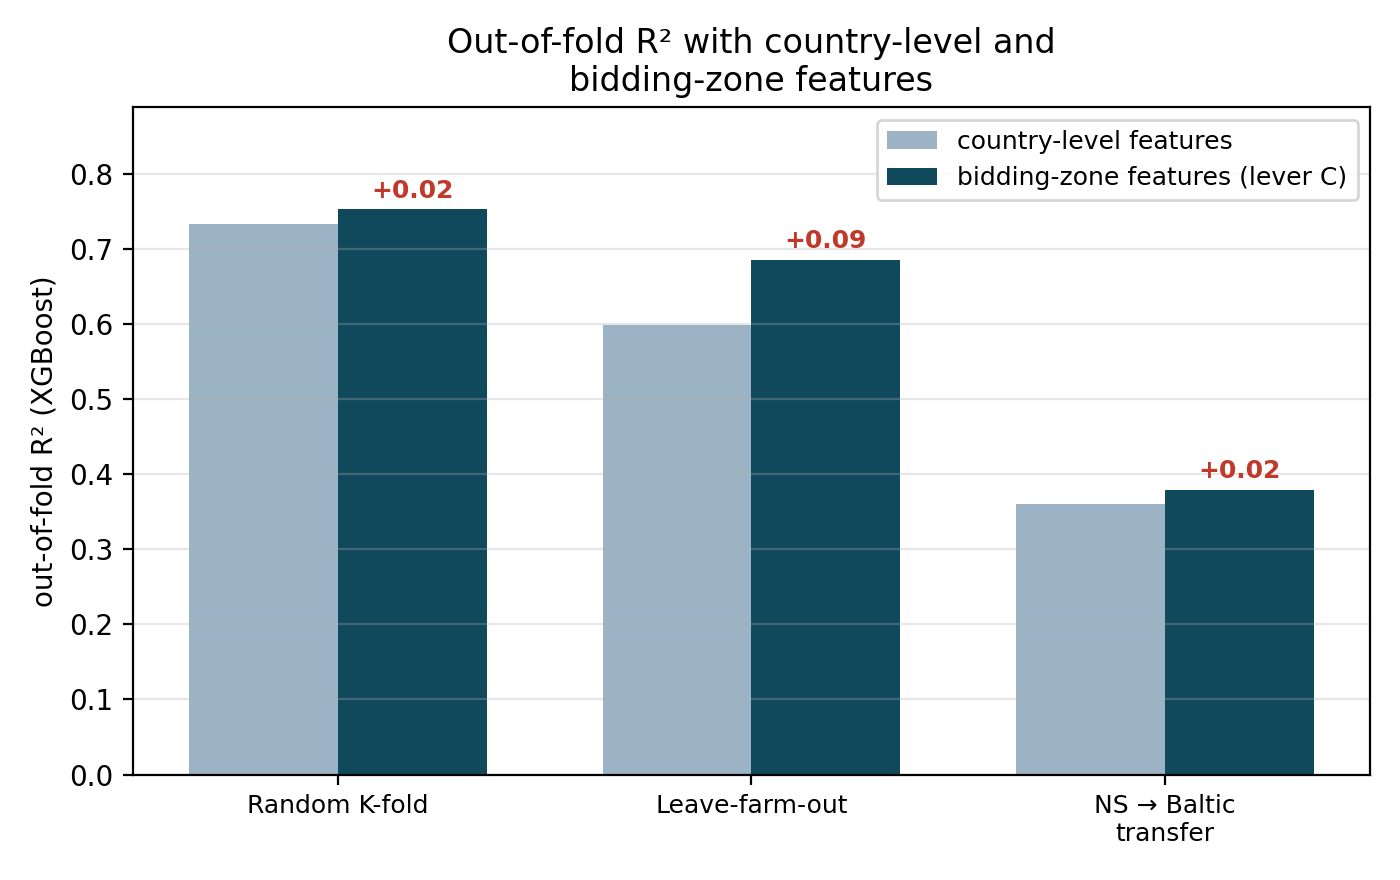
\includegraphics[width=0.7\textwidth]{fig_F_leverC_before_after}
    \caption{What bidding-zone resolution buys: out-of-sample $R^2$ before and
    after resolving features at the level prices form.}
    \label{fig:leverC}
\end{figure}

\begin{figure}[!htb]
    \centering
    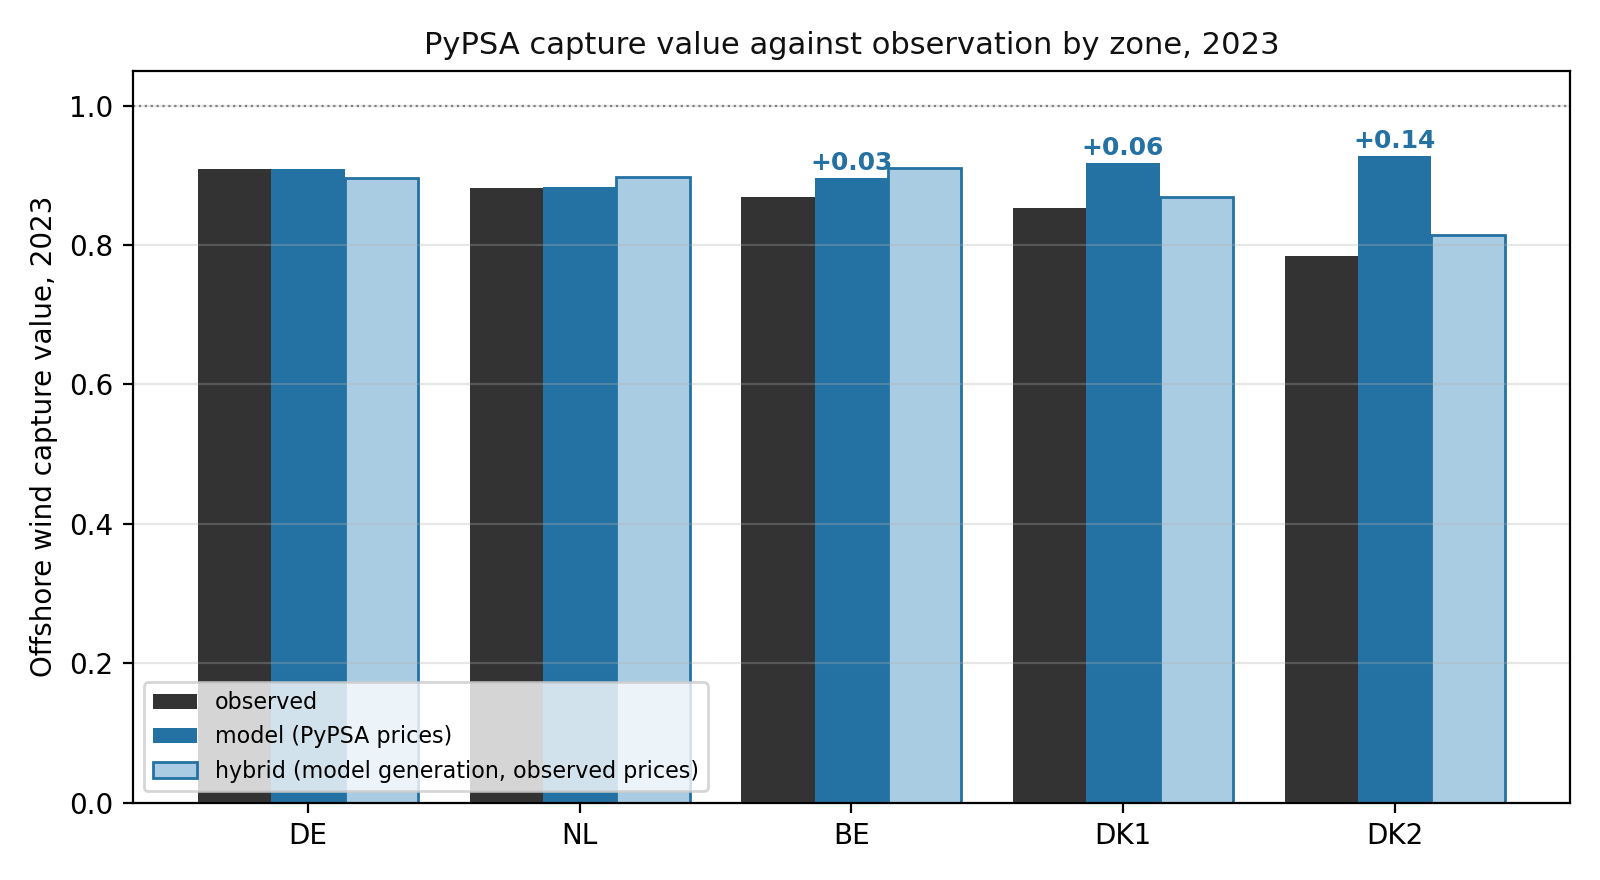
\includegraphics[width=0.85\textwidth]{fig_calibration_cv_2023}
    \caption{The system model's capture value, validated zone by zone for
    2023: observed, modelled, and the hybrid pairing modelled generation with
    observed prices. The model is near-exact in large zones and overstates
    capture value with congestion; the hybrid locates the error in the modelled prices and shows the modelled
    generation to be sound.}
    \label{fig:calibration_cv}
\end{figure}


\FloatBarrier
\subsection*{G.5 Robustness of the projection}

\begin{figure}[!htb]
    \centering
    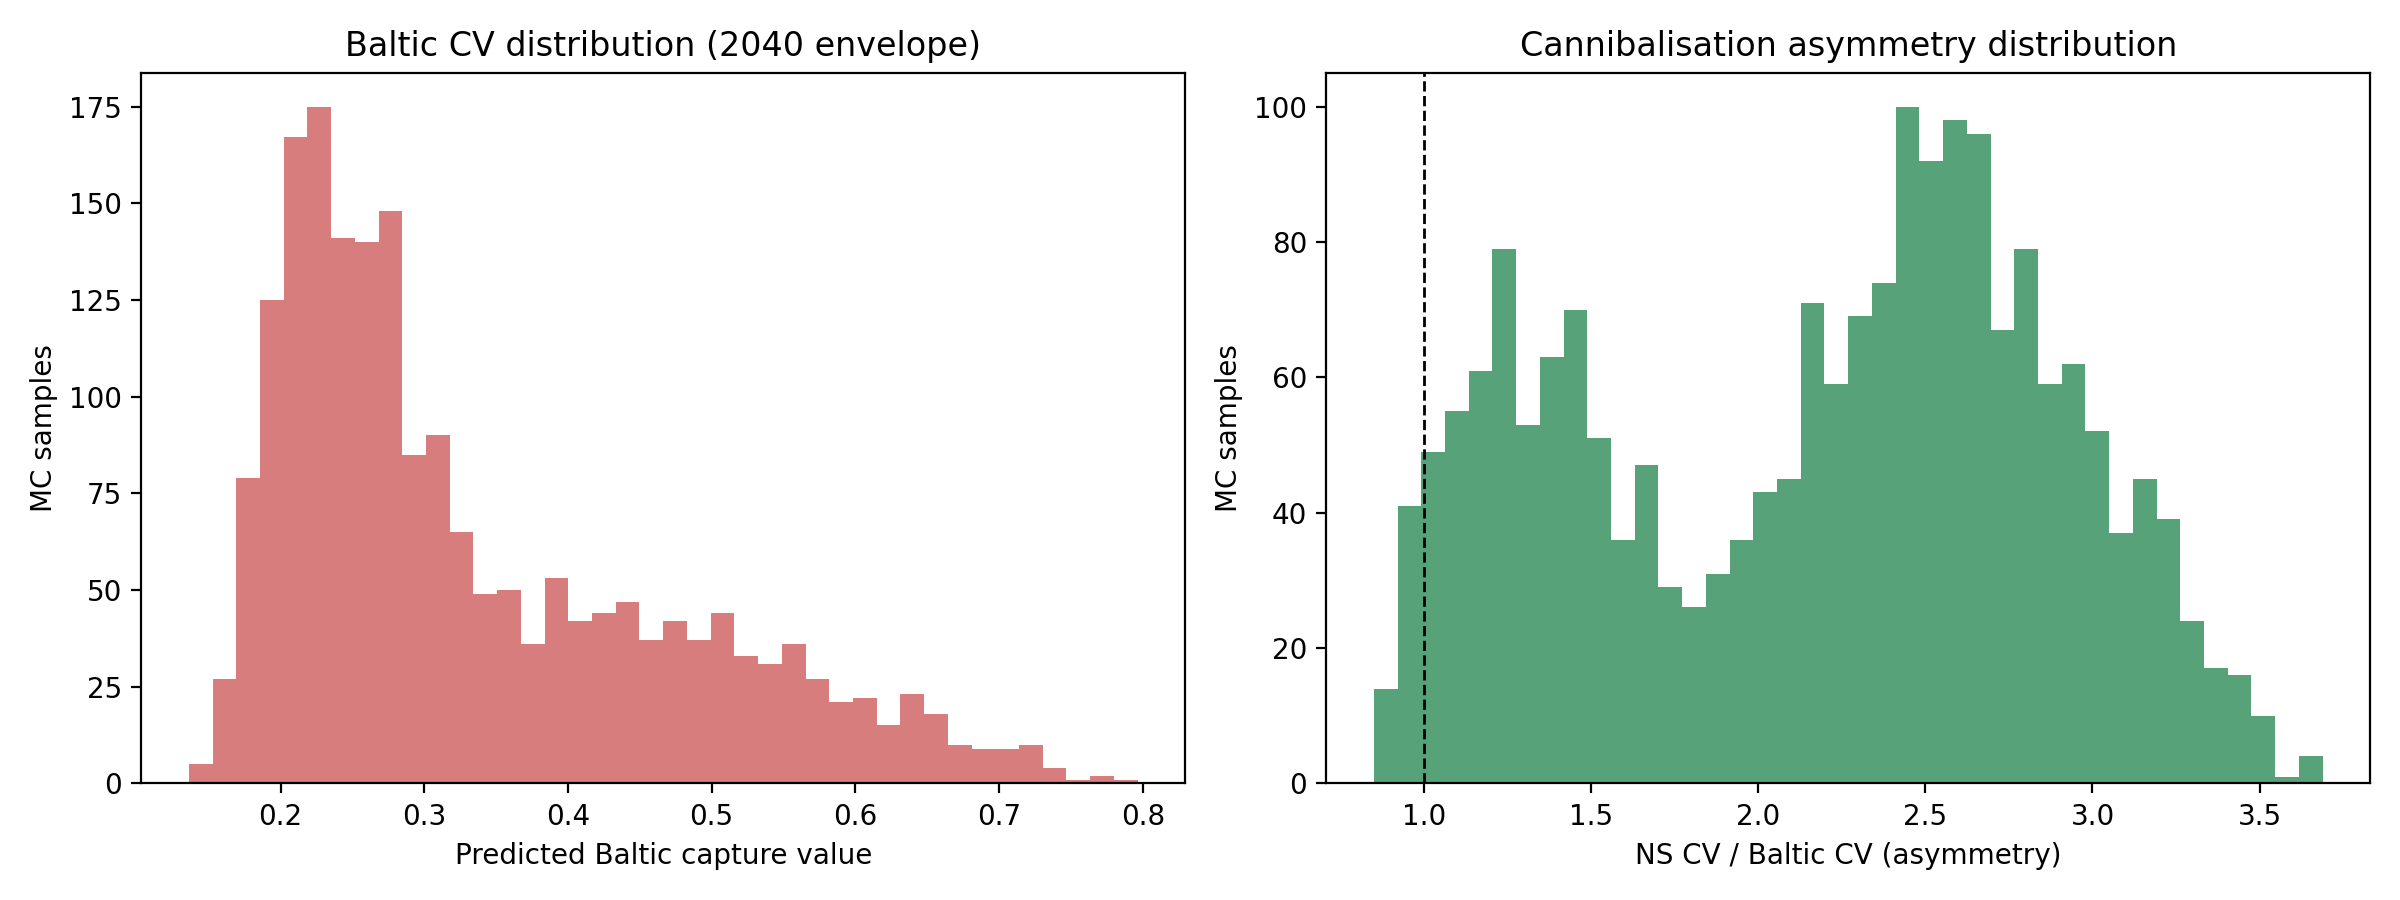
\includegraphics[width=0.85\textwidth]{fig_montecarlo}
    \caption{Monte-Carlo fans over the full input envelope (2,000 samples, inputs
    beyond TYNDP by design): Baltic capture value median 0.28, 90\,\% interval
    $[0.18, 0.62]$; North Sea to Baltic asymmetry median about 2.3$\times$. These figures describe the range of possibilities and give no single point
    result.}
    \label{fig:montecarlo}
\end{figure}

\begin{figure}[!htb]
    \centering
    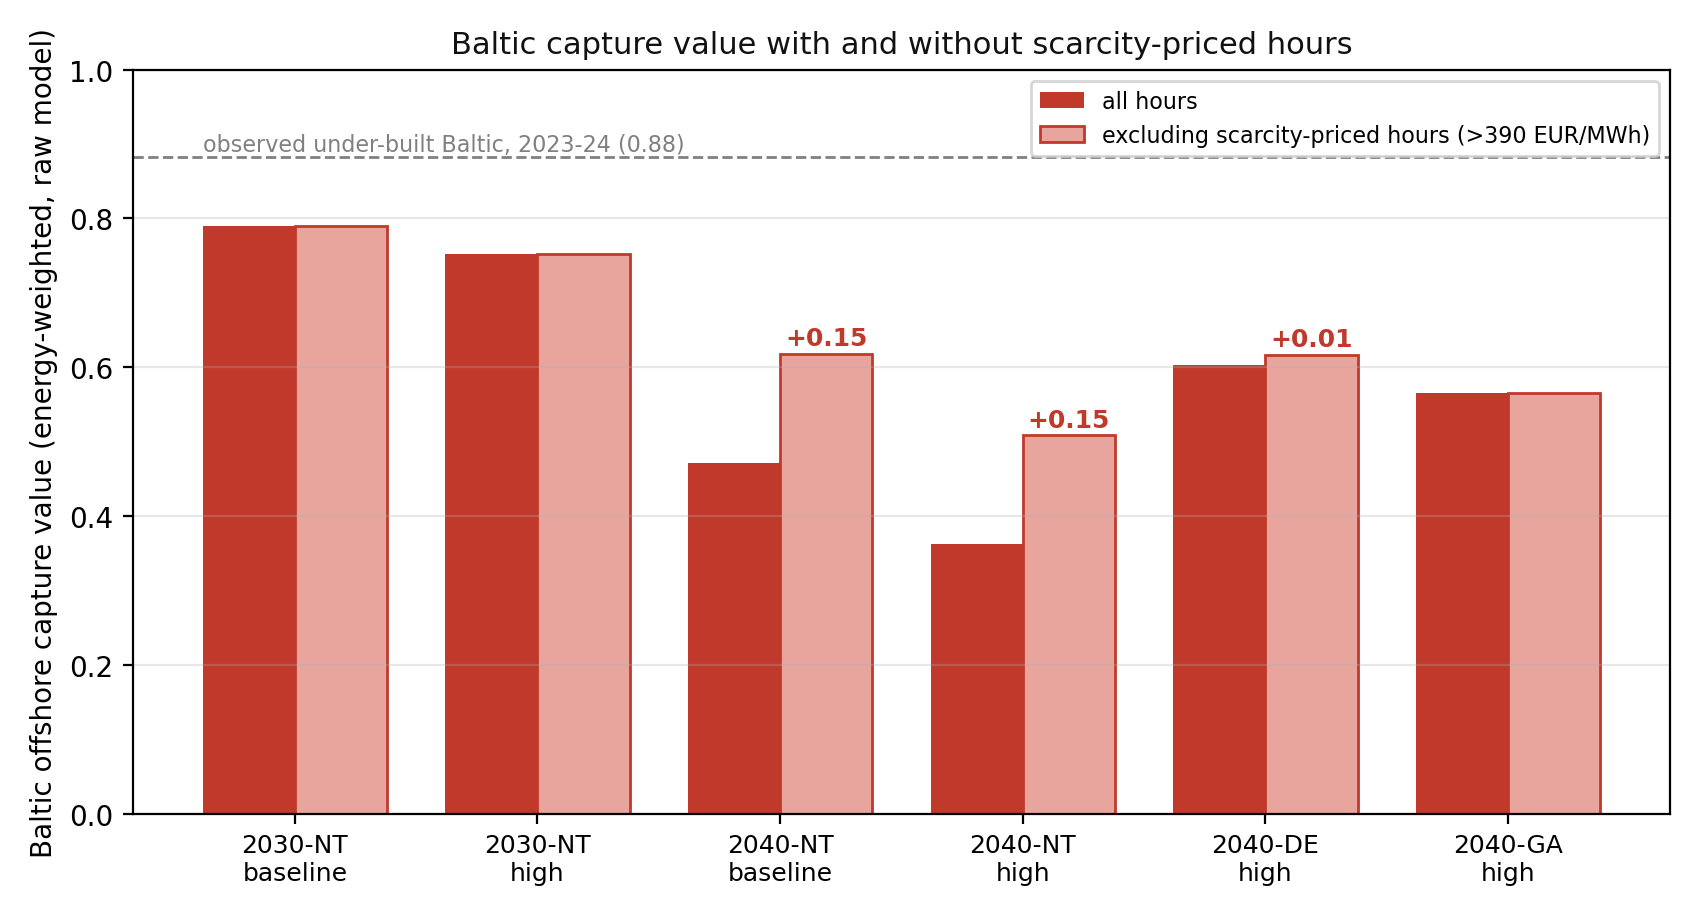
\includegraphics[width=0.9\textwidth]{fig_scarcity_bars}
    \caption{The fall survives the removal of scarcity-priced hours: Baltic capture value
    per scenario (uncorrected model), with and without scarcity-priced hours. The 2030 and clean 2040
    scenarios are scarcity-free; the NT 2040 scenarios carry a Polish adequacy
    component; severe erosion survives the exclusion in every case.}
    \label{fig:scarcity_bars}
\end{figure}


\begin{figure}[!htb]
    \centering
    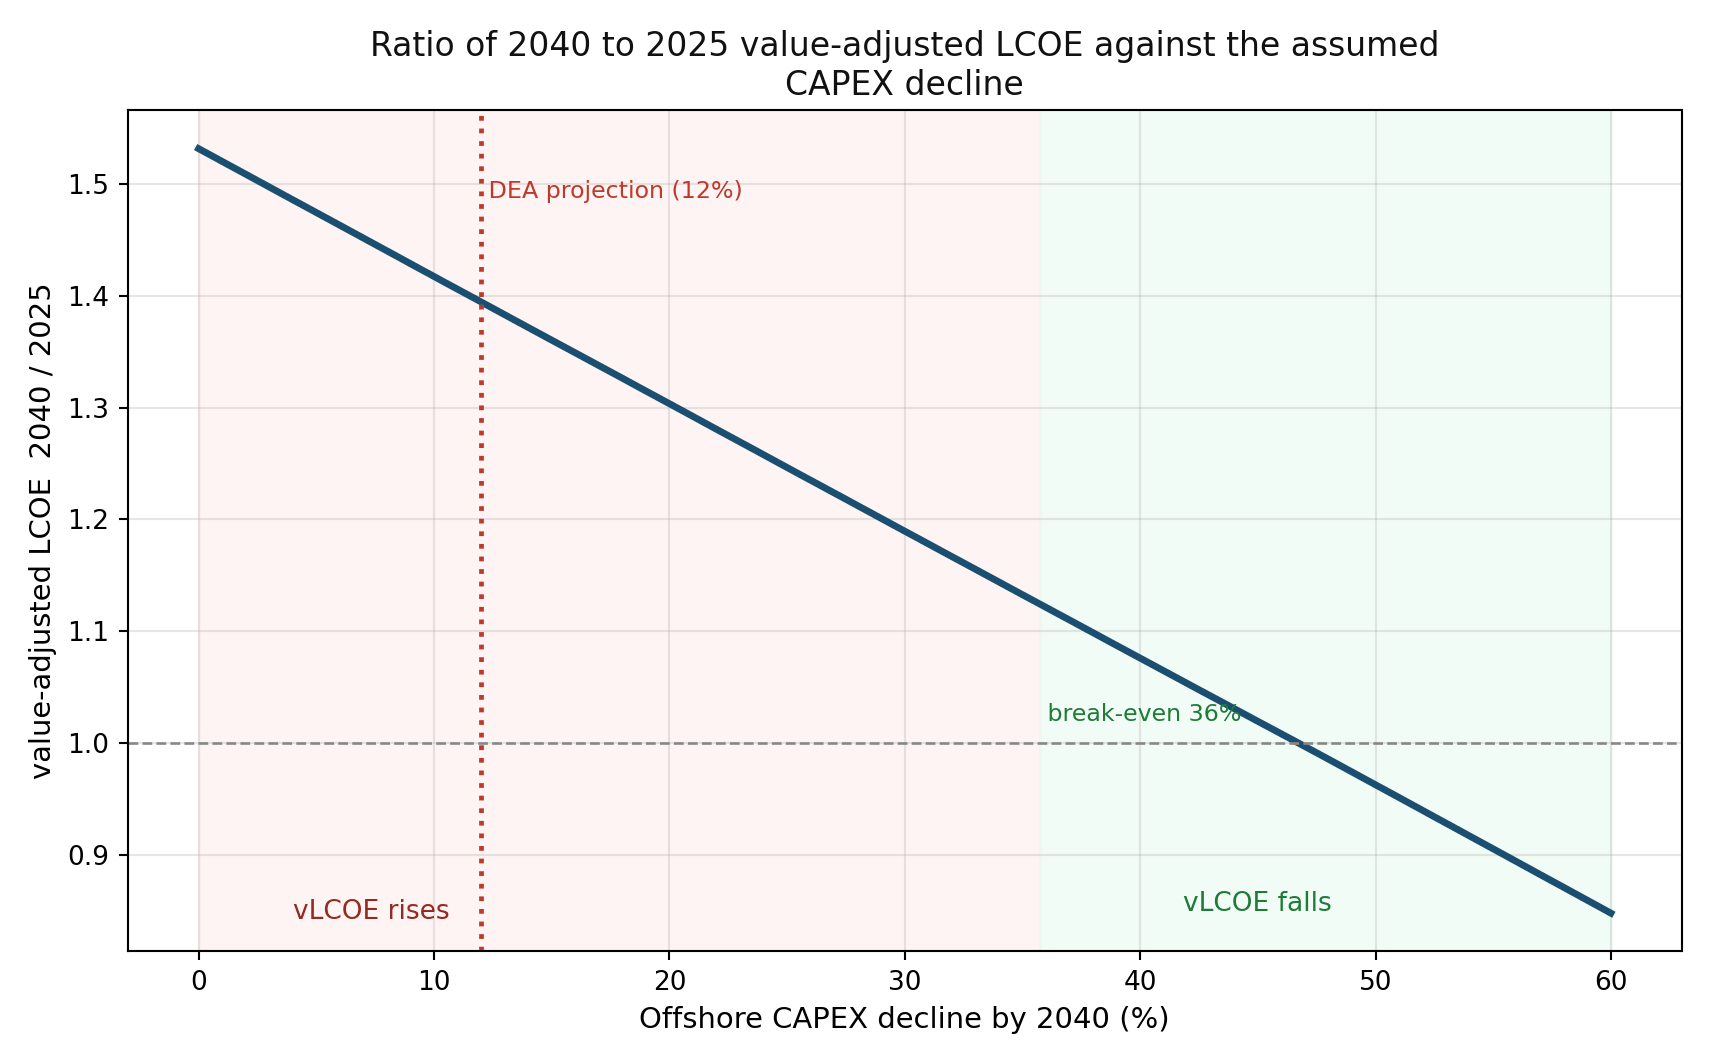
\includegraphics[width=0.82\textwidth]{fig_vlcoe_robustness}
    \caption{Robustness of the rising value-adjusted LCOE: the 2040-to-2025 ratio
    against the assumed offshore capital decline. It stays above one across the
    plausible range, and capital would have to fall about 36\%, against the
    database's 12\%, merely to hold the metric flat.}
    \label{fig:vlcoe_robust}
\end{figure}

\FloatBarrier
\subsection*{G.6 Mechanism: supporting detail}

\begin{figure}[!htb]
    \centering
    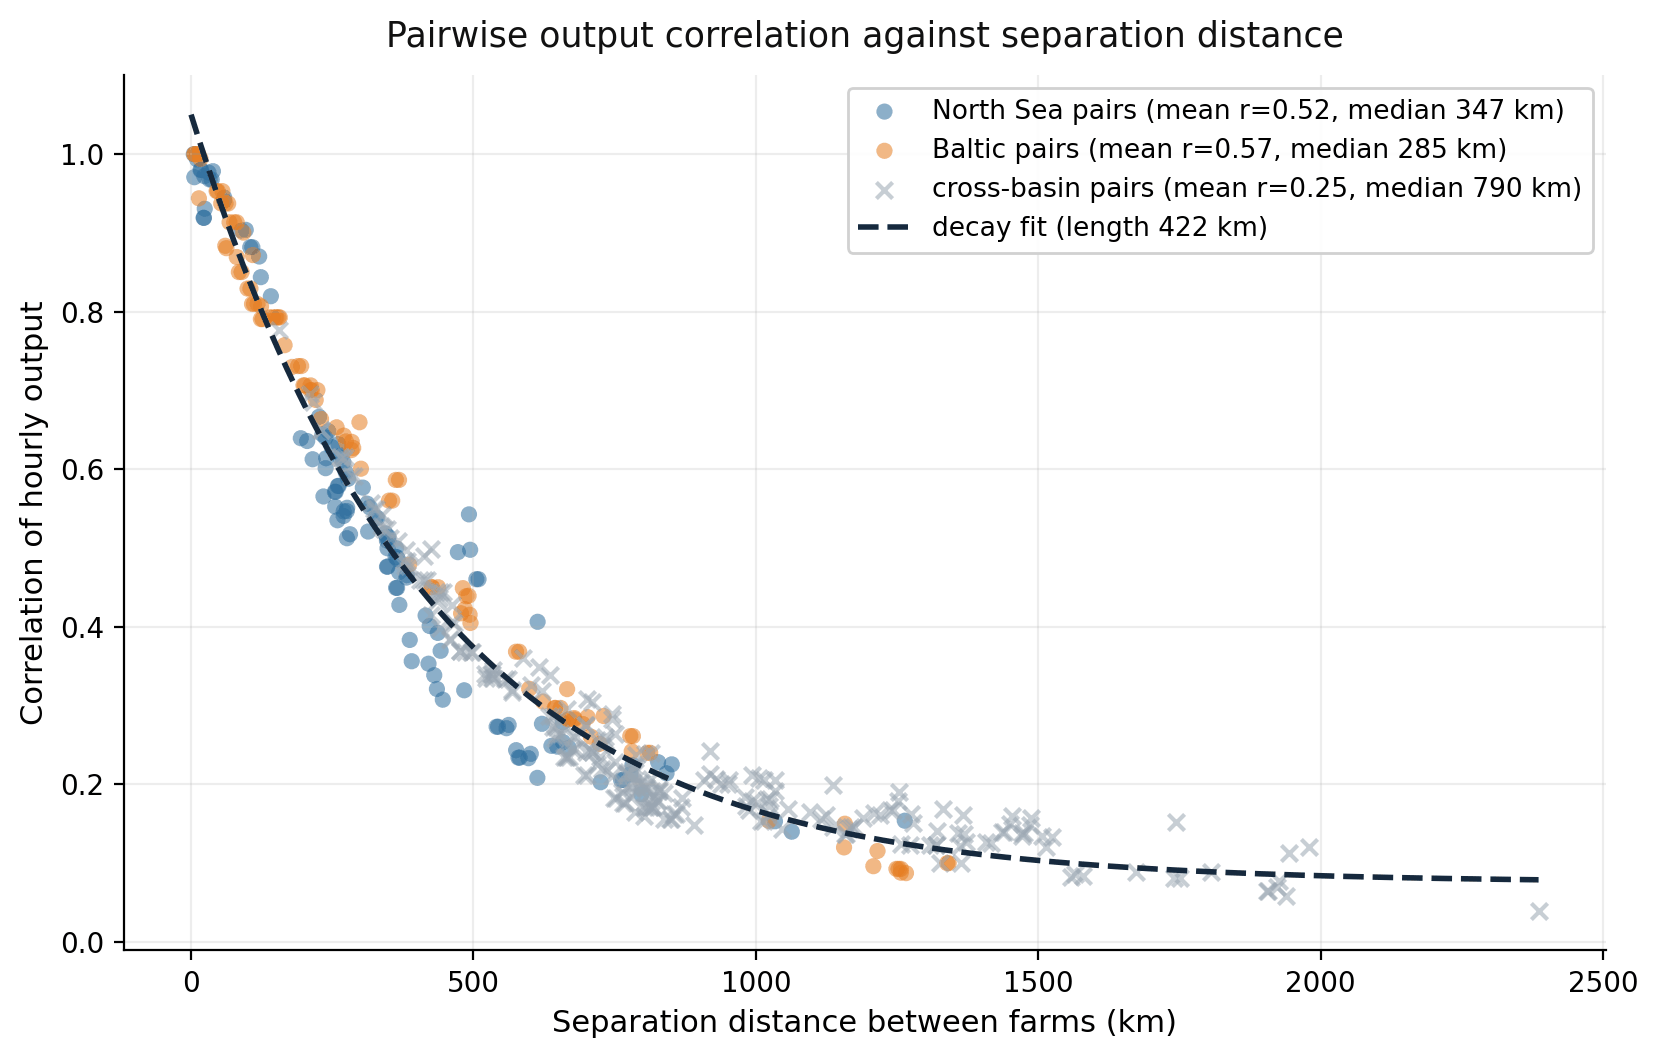
\includegraphics[width=0.78\textwidth]{fig_corr_vs_distance}
    \caption{Pairwise correlation of hourly wind output against separation
    distance, every farm pair, 2017 to 2024. All pairs follow one decay curve
    (fitted length 422~km); the Baltic pairs (mean 0.57) sit slightly above the
    North Sea pairs (mean 0.52), with a shorter typical separation (median 285
    against 347~km), while cross-basin pairs (mean 0.25) lie far out along the curve.}
    \label{fig:corr_distance}
\end{figure}

\begin{figure}[!htb]
    \centering
    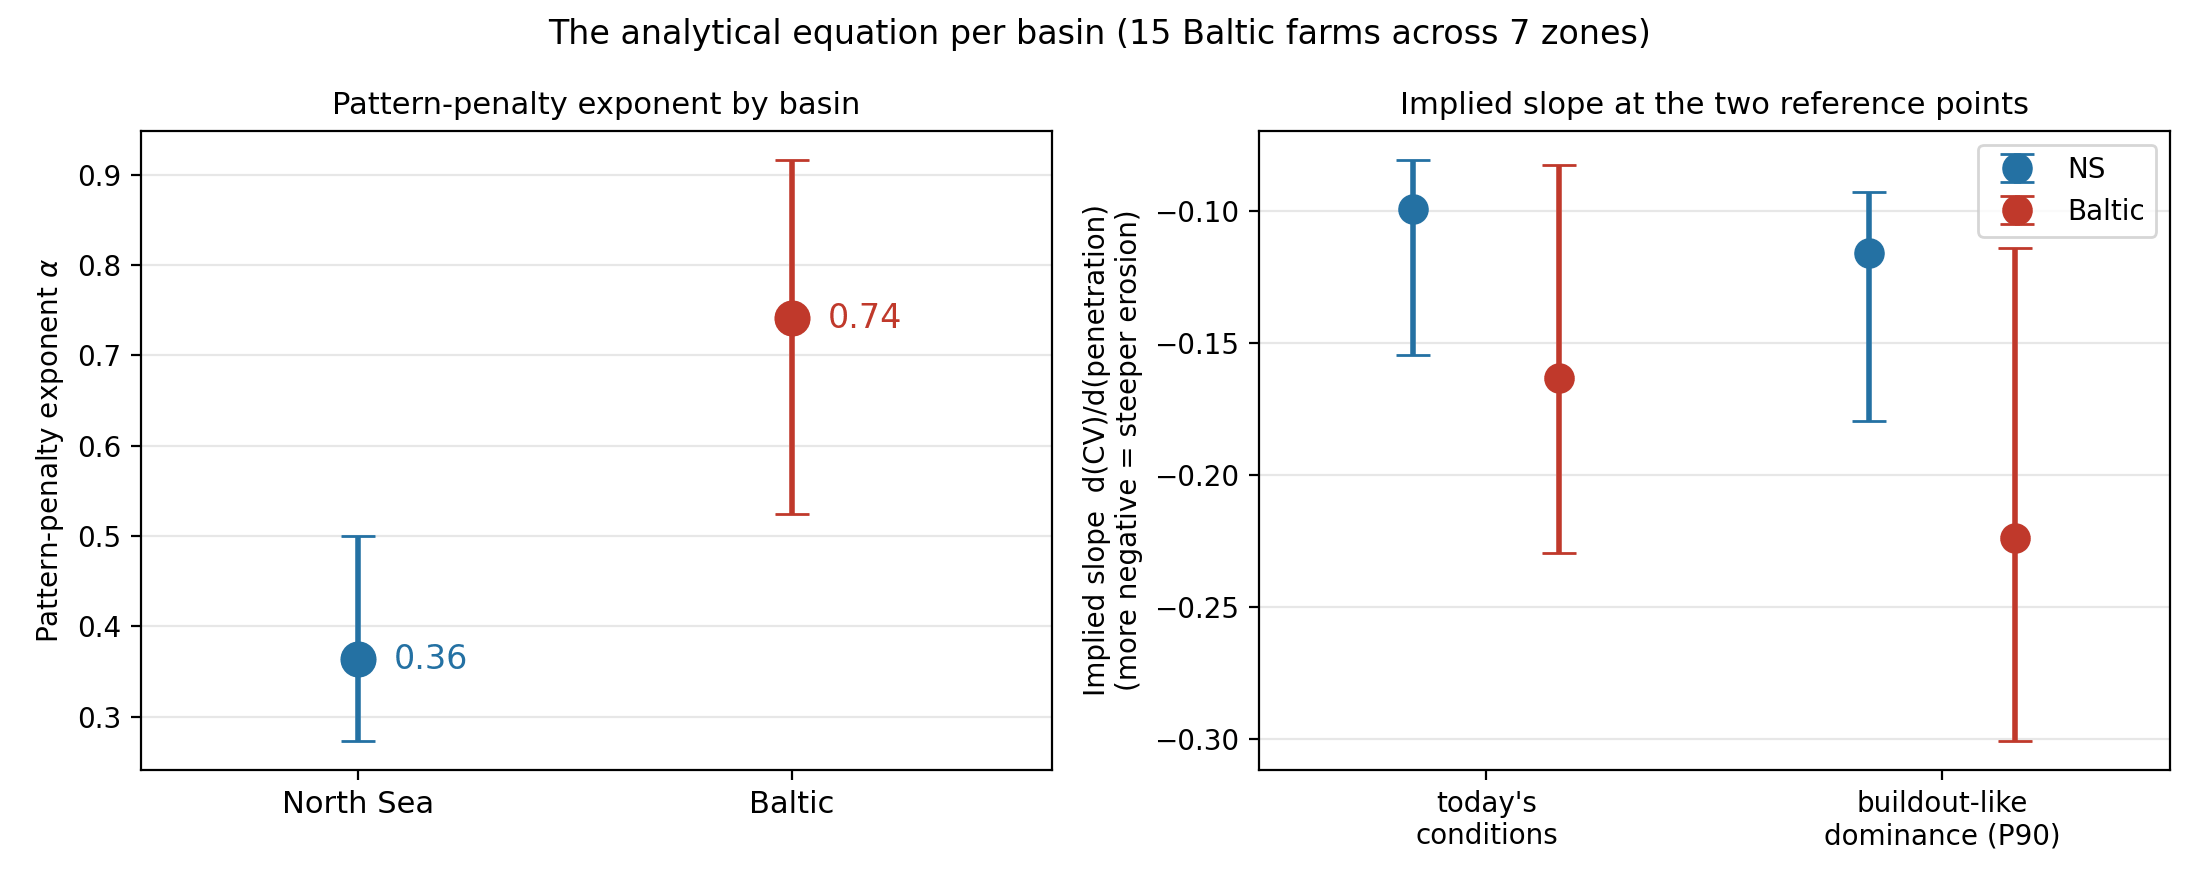
\includegraphics[width=0.9\textwidth]{fig_constants_comparison}
    \caption{The analytical equation refit per basin on the seven-zone panel
    (fifteen Baltic farms). Left: the pattern-penalty exponent is steeper in the
    Baltic (0.74 versus 0.37). Right: the implied slope of capture value against
    penetration is about 1.6 times steeper for the Baltic today and 1.9 times at
    buildout-like dominance. Whiskers are farm-block bootstrap 90\,\% intervals;
    the comparison is directional on a small panel.}
    \label{fig:constants}
\end{figure}



\end{document}
